\documentclass[a4paper, twoside]{book}

\usepackage[spanish, english, french]{babel} 

\usepackage[utf8]{inputenc}
\usepackage[T1]{fontenc}
%\usepackage{times}

%Configuration de la mise en page
%Menus des annexes
\usepackage{appendix}

%Gestion des images
\usepackage{graphicx}
\usepackage{wrapfig}
\addto\captionsfrench{\def\figurename{Image}}
\addto\captionsfrench{\def\tablename{Tableau}}

%Modifier taille légende des images
\usepackage[font=small]{caption}

%Note de bas de page
\counterwithout*{footnote}{chapter}

% Éléments de mise en page (marge de 2,5 cm, alinéa en début de paragraphe 1cm, interligne 1,5)
\usepackage{setspace}
\onehalfspacing
\setlength{\parindent}{1cm}
\usepackage[a4paper,margin=2.5cm]{geometry}
%Colonnes
\usepackage{paracol}

%%barrer du texte
\usepackage{soul}

%TABLEAU
\usepackage{longtable}
%pour mode paysage
\usepackage{lscape}
%Pour paysage dans le pdf
\usepackage{pdflscape}
%Utiliser couleurs dans un tableau
\usepackage{colortbl}
%gestion avancée des couleurs. On met nom de la couleur puis pourcentage
\usepackage{xcolor}
%Séparer une cellule en 2
\usepackage{diagbox}

\usepackage{epigraph}

%Pour avoir liens dans document (externes ou internes)
\usepackage{hyperref}
\hypersetup{pdfauthor={Lise Bernard},pdftitle={memoire_M2}, pdfborder=0 0 0}

%après hyperref : le paquet de glossaire PAS FONCTIONNEL
%\usepackage[automake,toc]{glossaries}
%\makeglossaries

%\newglossaryentry{broderie}{name=Broderie, description={technique d'ornementation qui consiste à ajouter à la surface d'un support un décor généralement exécuté à l'aiguille avec des fils et divers éléments.}}


%% Commande écriture inclusive
\newcommand{\inclusive}[1]{$\cdot${#1}}
\newcommand{\inclusives}[1]{$\cdot${#1}$\cdot${s}}

%commande siècle
\newcommand{\siecle}[1]{\textsc{#1}\textsuperscript{e} siècle}

%Commande pour vider le titre courant et pagination des pages vides (l'insérer sur page que l'on veut vider)
\newcommand{\clearemptydoublepage}{
	\newpage{\pagestyle{empty}\cleardoublepage}}
	
%Commande pour les citations de + de 3 lignes
\newenvironment{citer}{\quote\singlespacing\small\vspace{-6pt}}
{\endquote\doublespacing}

% Listes
\usepackage{enumerate}
\usepackage{enumitem}

%%Bibliographie
%TeXShop → Réglages → Éditeur → Complétions de BibDesk
% Pour avoir guillemets français dans biblio
\usepackage[babel]{csquotes} 
%paquet gestion biblio
\usepackage[backend=biber, isbn=false, doi=false, url=false]{biblatex-chicago}


\addbibresource{../bib/TextAndes.bib}
\addbibresource{../bib/ArchAnd.bib}
\addbibresource{../bib/projetText.bib}
\addbibresource{../bib/classificationTextile.bib}
\addbibresource{../bib/TextDigital.bib}
\addbibresource{../bib/SIG.bib}
\addbibresource{../bib/IDandine.bib}
\addbibresource{../bib/computervision.bib}

\DeclareSourcemap{
	\maps[datatype=bibtex]{
		\map[overwrite]{
			\perdatasource{../bib/TextAndes.bib}
			\step[fieldset=keywords, fieldvalue={,TextAnd}, append]
		}
	 \map[overwrite]{
			\perdatasource{../bib/ArchAnd.bib}
			\step[fieldset=keywords, fieldvalue={ArchAnd,}, append]
		}
        \map[overwrite]{
			\perdatasource{../bib/projetText.bib}
			\step[fieldset=keywords, fieldvalue={,projetText}, append]
		}
	\map[overwrite]{
			\perdatasource{../bib/classificationTextile.bib}
			\step[fieldset=keywords, fieldvalue={,classificationTextile}, append]
		}
	\map[overwrite]{
			\perdatasource{../bib/TextDigital.bib}
			\step[fieldset=keywords, fieldvalue={,TextDigital}, append]
		}
	\map[overwrite]{
			\perdatasource{../bib/SIG.bib}
			\step[fieldset=keywords, fieldvalue={,SIG}, append]
		}
	\map[overwrite]{
			\perdatasource{../bib/IDandine.bib}
			\step[fieldset=keywords, fieldvalue={,ID}, append]
		}
	\map[overwrite]{
			\perdatasource{../bib/computervision.bib}
			\step[fieldset=keywords, fieldvalue={,CV}, append]
		}
	}
}

%Run XeLaTeX puis BibTeX puis 2 fois XeLaTeX

\begin{document}
\frontmatter

\begin{titlepage}
\begin{center}

\bigskip

\begin{large}
UNIVERSITÉ PARIS, SCIENCES \& LETTRES
\end{large}
\begin{center}\rule{2cm}{0.02cm}\end{center}

\bigskip
\bigskip
\bigskip

\begin{Large}
\textbf{Lise Bernard}\\
\end{Large}
\begin{normalsize} \textit{licencié ès lettres}\\
\textit{Diplômée de Master en anthropologie de l'Amérique latine}\\
\end{normalsize}

\bigskip
\bigskip
\bigskip

\begin{Huge}
\textbf{Dynamiques de transmission des techniques et des iconographies dans les textiles andins sur la longue durée}\\
\end{Huge}
\bigskip
\bigskip
\bigskip

\bigskip
\bigskip
\bigskip
\begin{large}
\end{large}
\vfill

\begin{large}
Mémoire 
pour le diplôme de master \\
\og Humanités numériques et computationnelles \fg{} \\
\bigskip
2024
\end{large}

\end{center}
\end{titlepage}

\thispagestyle{empty}

\cleardoublepage

\section*{Résumé}
\addcontentsline{toc}{chapter}{Résumé}

\vspace{5pt}

À partir d'un corpus de 696 pièces textiles, ce mémoire examine les mobilités et les imitations techniques et iconographiques dans les tissages andins. Ce travail met en parallèle une approche géographique des mobilités textiles, à partir des métadonnées géographiques dont nous disposons sur ces textiles, et une approche de vision par ordinateur, à partir des images des textiles. Le recours à ces outils numériques variés permet de comparer les échanges textiles avec les phénomènes de ré-interprétations techniques et iconographiques, dans une approche diachronique sur la longue durée depuis 1800 avant J.C. jusqu’à la période contemporaine.

\medskip

\textbf{Mots-clés:} Textile; Tissage; Andes; Pérou; Bolivie; Humanités Numériques; Système d'Informations Géographiques; Apprentissage Machine; Vision par ordinateur.

\textbf{Informations bibliographiques:} Lise Bernard, \textit{Dynamiques de transmission des techniques et des iconographies dans les textiles andins sur la longue durée}, mémoire de master 2 \og Humanités numériques et computationnelles\fg{}, dir. Astrid Castres et Daniel Stockholm, Université Paris, Sciences \& Lettres, 2024.

\vspace{5pt}

\section*{Abstract}
\addcontentsline{toc}{chapter}{Abstract}

Based on a corpus of 696 textile pieces, this dissertation examines mobilities and technical and iconographic imitations in Andean weaving. This work combines a geographical approach to textile mobility, based on the geographic metadata we have on these textiles, and a computer vision approach, based on images of the textiles. The use of these varied digital tools makes it possible to compare textile exchanges with the phenomena of technical and iconographic re-interpretations, in a diachronic approach over the long term from 1800 BC to the contemporary period.

\medskip

\textbf{Keywords:} Textile; Weaving; Andes; Peru; Bolivia; Digital Humanities; Geographic Information System; Machine Learning; Computer Vision.

\textbf{Bibliographic Information:} Lise Bernard, \textit{Dynamics of Transmission of Techniques and Iconographies in Andean Textiles over the long term}, M.A. thesis \og Digital and computational humanities\fg{}, dir. Astrid Castres and Daniel Stockholm, Université Paris, Sciences \& Lettres, 2024.


\clearpage
\thispagestyle{empty}
\cleardoublepage

\section*{Remerciements}

\epigraph{\textquotedblleft Antes de realizar investigaciones de campo, hay que tener en cuenta que los pasajes de esta categoría de viajes no incluyen automáticamente un boleto de vuelta con respeto a la dimensión psico-cultural.\textquotedblright}{E. Fischer, 2008, \textit{Urdiendo el tejido social: sociedad y producción textil en los Andes bolivianos}, p.~30-31.}

\vspace{30pt}

	Tout d'abord, je voudrais remercier mes deux directeurs de recherche. Mme Astrid Castres qui a pris le temps de se plonger dans les Humanités Numériques, et M. Daniel Stockholm pour son aide dans la découverte de l'analyse de l'image et son intérêt pour ce corpus de textiles andins.
    
\begin{center}
   ***
\end{center}

	Je tiens aussi à remercier les professeurs de l'École Nationale des Chartes auprès desquels je me forme aux Humanités Numériques dans un cadre bienveillant et stimulant. Merci à tous ceux qui ont pris le temps de m'accompagner sur ce projet, et tout particulièrement à Mme Carmen Brando et M. Chahan Vidal-Gorène pour les nombreux échanges qui ont enrichi ce mémoire. Je suis également reconnaissante envers M. Lucas Terriel pour son aide sur le \textit{webscrapping} de la base de données. \\
	
	Un grand merci à Nicolas Goepfert et Romuald Housse, leurs regards d'archéologues m'ont guidée dans le dédale des chronologies et des zones géographiques des Andes. Et enfin, une pensée toute particulière pour Mme Sophie Desrosiers, qui m'a introduite à l'univers des textiles andins à la fois par l'ensemble merveilleux de ses travaux et par ses ateliers de tissage andin.

\begin{center}
   ***
\end{center}

Je suis également très reconnaissante envers mes camarades de classe, sans qui cette année n'aurait pas été la même. Merci aux ami\inclusives{e}, toutes les personnes qui ont rendu ces mois de travail ardu, plus légers. À ma famille, pour son soutien au quotidien et ce malgré la distance. Mélissa, dans celui-ci tu trouveras bien \og nonobstant \fg. Et évidemment à Alice, \textit{chica valiente}, dont la présence, même à des milliers de kilomètres, m'est indispensable.

\begin{center}
   ***
\end{center}

Enfin, ce mémoire est tout particulièrement dédié à tous les tisserands et toutes les tisserandes dont j'ai croisé le chemin dans les Andes et qui ont accepté de m'introduire à leurs savoir-faire.

\clearpage
\thispagestyle{empty}
\cleardoublepage

% table des matières
\renewcommand{\contentsname}{Sommaire}
\tableofcontents
\markboth{}{}{}

\clearpage

\mainmatter

\chapter*{Glossaire des termes textiles\footnote{Ce glossaire a été réalisé à partir des sources suivantes : \begin{itemize} \item A. Castres et T. Gaumy, \textit{La fabrique de l'habit: artisans, techniques et production du vêtement (XVe-XVIIIe siècle)}, Paris, École des chartes, 2020. \item Centre International d'Étude des Textiles Anciens, \textit{Vocabulaire technique français}, Lyon, CIETA, 2020. \item I. Emery, \textit{The primary structures of fabrics: an illustrated classification}, Londres, Paris, Thames and Hudson, The Textile Museum, 1995[1966]. \item A. Leroi-Gourhan, \textit{L'Homme et la Matière : évolution et techniques}, Paris, Albin Michel, 1943. \end{itemize} }}
\addcontentsline{toc}{chapter}{Glossaire}

\begin{itemize}
	\item \textbf{Tissage} : Assemblage de deux nappes d'éléments perpendiculaires, l'une longitudinale nommée \textbf{chaîne} et l'autre transversale nommée \textbf{trame}. 
\end{itemize}

\vspace{10pt}

 \begin{itemize}
 	\item \textbf{Armure textile ou structure textiles} : Manière dont les fils sont entremêlés.
	\item \textbf{Broderie} : Technique d'ornementation qui consiste à ajouter à la surface d'un support un décor généralement exécuté à l'aiguille avec des fils et divers éléments.
	\item \textbf{Chaîne ou trame supplémentaire} : Groupe d'éléments supplémentaires parcourant le tissu dans le sens de la trame ou de la chaîne et répondant à une fonction distincte : création de motifs, effet de texture, renforcement du tissage...
	\item \textbf{Double-étoffe} : Tissu composé de deux tissages distincts l'un au-dessus de l'autre, échangeant fréquemment leurs positions respectives dans le tissu.
	\item \textbf{Flotté} : Tout fil de trame ou de chaîne qui passe au dessus de plus d'un fil de l'élément opposé.
	\item \textbf{Lisière} : Bord d'un tissu.
	\item \textbf{Réseau} : Tissu composé d'un fil unique qui s'enlace ou se noue sur lui-même.
	\item \textbf{Tissage équilibré ou toile} : tissage composé d'une seule trame et d'une seule chaîne, donc chaque fil passe successivement au-dessus puis au-dessous des éléments opposés, sans flottés.
	\item \textbf{Tissage face chaîne ou dominante chaîne} : Tissage au sein duquel le nombre et la densité des fils de chaîne font qu'ils cachent entièrement les fils de toile.
	\item \textbf{Tissage face trame ou dominante trame ou tapisserie} : Tissage au sein duquel le nombre et la densité des fils de trame font qu'ils cachent entièrement les fils de chaîne.
\end{itemize}
\addcontentsline{toc}{chapter}{Glossaire}

\chapter*{Introduction}
\addcontentsline{toc}{chapter}{Introduction}
\setlength{\columnsep}{3em}

\footnotelayout{m} \begin{paracol}{2}
 \noindent  \og Parce qu'il y a beaucoup de gens dans mon pays qui ne savent plus ce qu'est Paracas, ce qu'est Huari, et Chancay et Nazca, tu vois ? Presque plus personne ne sait maintenant. Donc nous som- mes, je suis pour la diffusion, et je suis pour l'enseigner, tu vois ? Pour qu'ils puissent apprendre, pour qu'ils puissent me connaître, connaître mon travail ou le travail que nous faisons depuis les ancêtres tu vois ? [...] C'est qu'au Pérou, il y a beaucoup, beaucoup de lieux qui ont fait [des textiles] comme Huari, comme Nazca, comme Chancay et comme Paracas. [...] Alors, c'est pour ça que les gens et nous travaillons. Parce que nous ne voulons pas perdre l'essence que nous a laissée l'héritage, nos ancêtres, tu vois \footnote{Entretien avec Ciriaco, 13 mars 2022, Ayacucho (Pérou).} ? \fg \\
    
    \switchcolumn
    
    \textquotedblleft \textit{Porque hay mucha gente en mi país ya no saben qué cosa es Paracas, qué cosa es este Huari ?`no? y Chancay y este Nazca?`no? Casi nadie saben ya no. Entonces nosotros estamos esta, yo estoy esta para difundir y yo estoy para enseñarla ?`no?, para que puedan aprender, para que pueden conocer a mi, a mi, a mi trabajo o el trabajo que hacemos desde los ancestros ?`no? [...] Es que en Perú, hay muchos, muchos lugares que, que hubo [tejidos] pues como Huari, como Nazca, como Chancay y como Paracas. Entonces hay muchas leyendas de tejido. Muchas leyendas. [...] Entonces, hacia eso la gente o nosotros trabajamos ?`no? Porque no quisiéramos perder esa esencia que nos ha dejado la herencia, el antepasado ?`no?}\textquotedblright\\
\end{paracol}


Ciriaco, tisserand à Ayacucho dans les Andes centrales péruviennes, ancre son travail d'artisan textile dans la continuité d'une longue tradition. Lors de cette discussion, il présente le textile comme vecteur de l'héritage préhispanique en l'inscrivant dans la lignée de civilisations disparues : Paracas, Huari, Chancay ou Nazca. Le textile qu'il produit est commercialisé comme artisanat péruvien mais également présenté comme héritier de ces cultures préhispaniques dont Ciriaco se revendique descendant\footnote{Les entretiens ethnographiques ne peuvent être compris hors de la manière dont les enquêté\inclusives{e} souhaitent être perçus. Quelques minutes avant d'aborder cette thématique, Ciriaco me demande si je suis toujours en train d'enregistrer, il a conscience que le discours qu'il me tient restera gravé et présente possiblement ce qu'il pense que j'attends de cette discussion.}.
	
Ce discours de continuité de la pratique textile est fortement développé au Pérou, et plus largement dans les Andes, car une multitude de textiles a été retrouvée lors des nombreuses fouilles archéologiques qui ont eu lieu depuis le milieu du \siecle{xx}. Si ces découvertes sont possibles c'est notamment grâce au climat désertique le long de la côte péruvienne qui offre des conditions de conservation idéale pour les fibres animales et végétales qui composent les pièces textiles\footnote{\cite[p.~263]{desrosiersTechniquesTissageOntelles2010}}. À l'inverse, les civilisations des hautes-terres de la Cordillère des Andes (ou \textit{sierra}) ont été productrices de textiles, mais le climat humide et froid en altitude n'a pas permis leur conservation --- à part quelques échantillons retrouvés sur des momies découvertes au-dessus de 5000 mètres d'altitude et dont les vêtements ont été conservés par la congélation\footnote{\cite{abalderussoArteTextilIncaico2010}}--- .
\noindent Ces textiles perdurent sur la longue durée, puisqu'ils composent un témoignage de cultures matérielles s'étendant sur plus d'un millénaire, et sont encore inscrits dans l'imaginaire des tisserand\inclusives{e} contemporain\inclusives{e} comme l'illustre le discours de Ciriaco. \\


\section*{État de l'art}

\subsubsection*{La foisonnante étude des textiles andins}

L'abondance des textiles andins, leur complexité et leur ancienneté génèrent, comme le souligne Annabel Vallard, \og une passion internationale et une bibliographie abondante \fg\footcite[p.~1]{vallardSilvermanGailWoven2009}.

Dès les années 1930, les études américanistes se concentrent sur les découvertes archéologiques préhispaniques, y compris sur le textile. Lila O'Neale et Alfred Kroeber proposent ainsi, dans un recueil en majeure partie composé de planches photographiques, des pistes d'analyse des textiles archéologiques découverts sur la côte péruvienne au début du \siecle{xx}\footcite{onealeTextilePeriodsAncient1930}. 
Dès ces premiers travaux de recensions des fouilles, les archéologues développent une volonté classificatoire, notamment selon les cultures pré-hispaniques. En France, Raoul D'Harcourt, précurseur de l'ethnographie andiniste française, propose une analyse des textiles archéologiques du Pérou et de leurs techniques en 1934, cette analyse reste une référence dans le domaine\footcite{harcourtTextilesAnciensPerou2008}. Il s'applique à montrer la complexité des techniques utilisées par les populations préhispaniques et en propose une typologie. Une grande partie de l'analyse du textile, y compris dans le champ andiniste, consiste alors à penser la classification des artefacts. André Leroi-Gourhan, en 1943, dans sa classification générale des techniques, analyse les moyens de production textiles, y compris ceux utilisés dans les Andes. Il classe les textiles dans la catégorie des \og solides souples \fg\:composés d'élément ayant une \og flexibilité permanente qui permet de les assembler par intrication mutuelle \fg \footcite[p.~243]{leroi-gourhanHommeMatiereEvolution1943}. 
Sophie Desrosiers, spécialiste française des textiles andins, se montre critique face à cette classification. Elle souligne que Leroi-Gourhan se contredit dans son étude du textile puisqu'il promeut une classification des techniques à partir des matières premières, mais, pour le textile, il classifie les pièces selon l'assemblage des fibres et non leur composition. En 1966, Irene Emery propose une classification générale des techniques textiles selon l'entrecroisement des fils, accompagnée de photographies et intitulée \textit{The Primary Structure of Fabrics}\footcite{emeryPrimaryStructuresFabrics1995}. Cet ouvrage devient la référence en matière de classification textile et est encore aujourd'hui largement utilisé. Elle prend d'ailleurs des exemples d'armures textiles à partir de pièces archéologiques découvertes au Pérou. Nous pouvons aussi nous référer à l'ouvrage d'Annemarie Seiler-Baldinger pour une classification généraliste du textile selon son mode de production\footnote{\cite{seiler-baldingerTextilesClassificationTechniques1995}.\\Pour le débat sur les différentes proposition de classification textile, voir : \cite{balfetOuSontClassifications1988}}. Ces différentes approches classificatoires, depuis le début du \siecle{xx}, ne sont pas standardisées puisqu'elles ne reposent pas sur les mêmes fondements théoriques. Or, face à la massification des données, quel est le meilleur compromis pour organiser les textiles entre eux sans perdre d'informations ? 

Dans les années 1980, on assiste à une reviviscence de l'analyse des textiles andins. L'anthropologie s'est longtemps intéressée au textile en tant qu'objet et, surtout, comme un objet appartenant au passé, produit par des populations disparues. Toutefois, au début du \siecle{xx}, certaines de ces techniques textiles étaient toujours existantes dans les communautés indigènes, notamment dans les hautes-terres andines. À partir de la fin du \siecle{xx}, les chercheurs et chercheuses s'intéressent donc moins aux textiles archéologiques et à leurs structures qu'aux textiles ethnographiques en eux-mêmes et comme outils de compréhension des textiles archéologiques. Par exemple, Sophie Desrosiers propose la reconstitution d'une ceinture dont le tissage est présenté dans une chronique de Fray Martín de Murúa  au \siecle{xvii}, \textit{Historia del origen y genealogía de los Reyes Incas del Perú} et dont elle a retracé une partie de l'existence jusqu'à l'époque contemporaine\footcite{desrosiersExperienceTechnologieReconstruction1985}. Retracer les évolutions des techniques est une des méthodes proposées par cette même chercheuse pour comprendre les textiles des hautes-terres dont nous avons peu de preuves archéologiques. Puisqu'il est en effet attesté que les textiles andins ont circulé, l'analyse des artefacts découverts sur la côte permettrait de comprendre ce qu'étaient ces textiles. Deux théories principales s'opposent sur cette question. D'une part, les partisans de l'influence principale des hautes-terres sur les régions côtières\footcite{desrosiersHighlandComplementaryWarpWeaving2014}, d'autre part, les tenants d'une influence principale inverse, depuis la côte vers l'Est \footcite{arnoldCienciaTejerAndes2019}. De nouvelles méthodes pourraient-elles nous permettre d'observer les influences mutuelles entre ces deux zones géographiques ? \\

L'histoire est également un domaine fertile pour comprendre l'inscription du textile dans les sociétés andines. 
À la période moderne, les colons espagnols qu'ils soient \textit{conquistadores} ou religieux importent l'écriture et rédigent des témoignages précieux sur les pratiques textiles incaïques. Une partie de ces textes sont des chroniques ; des ouvrages rédigés à la période coloniale par des colons ou par des métis, qui contiennent des descriptions de la colonisation, du mode de vie des habitants colonisés, de la géographie ou de la faune et de la flore locale, ainsi que des récits historiques rapportés par les populations locales. Dès les premières chroniques, la présence du textile est soulignée et largement décrite par les colons et métis. Ces récits historiques sont une source de compréhension des textiles produits dans les hautes-terres dans l'empire Inca et à la période coloniale. John Murra, anthropologue étatsunien de renom, spécialiste de la période inca, développe ainsi une analyse des pratiques textiles incaïques documentée essentiellement à partir des chroniques\footcite{murraClothItsFunctions1962}.

L'influence coloniale européenne sur les pratiques textiles andines a d'abord été étudiée à partir de la thématique des \textit{obrajes}. Quelques auteurs proposent des analyses sur l'introduction de nouvelles races ovines et du métier à pédale au sein des \textit{obrajes}, manufactures textiles destinées à la production de tissus domestiques. En 1964, Silva Santiesteban propose une analyse généraliste du fonctionnement des \textit{obrajes}\footcite{silvasantistebanObrajesVirreinatoPeru1964}. Les analyses lui succédant sont souvent plus localisées. Miriam Salas Olivari, dans les trois tomes de \textit{Estructura colonial del poder español en el Perú : Huamanga (Ayacucho) a través de sus obrajes. Siglos XVI-XVIII}, propose ainsi une analyse complète du système des \textit{obrajes} dans la région d'Ayacucho (Pérou)\footcite{salasolivariEstructuraColonialPoder1998}. Javier Ortiz de la Tabla Ducasse se concentre sur les \textit{obrajes} de Quito (Équateur) \footcite{ortizdelatabladucasseObrajesObrajerosQuito1982} et Mary Money sur ceux de la province de Charcas (Bolivie)\footcite{moneyObrajesTrajeComercio1983}. Ces différents travaux sur les \textit{obrajes} restent limités et ne détaillent pas forcément les techniques textiles, au profit de l'inscription politique et sociale de ces manufactures. En outre, leur histoire est reconstruite à partir des archives et donc principalement par les témoignages des élites, ce qui ne permet pas de saisir l'influence de ces nouvelles pratiques textiles sur les populations locales. Les Indépendances marquent la fin des \textit{obrajes}, et la production textile cesse d'intéresser les historien\inclusives{ne}, alors même qu'elle perdure dans les communautés de manière \og traditionnelle\fg \:et industriellement pour les vêtements de ville. 

Les \textit{obrajes} sont un élément central de la compréhension des modifications des pratiques textiles à la période coloniale. Toutefois, cette dernière avait tendance à être perçue comme un moment de rupture pour la zone andine, y compris du point de vue des pratiques textiles. Or, depuis les années 1990, des travaux s'attellent à nuancer l'influence européenne, notamment à travers la compréhension des phénomènes de métissage. En effet, à partir de la colonisation du continent, les pratiques textiles ne peuvent être pensées hors de l'histoire des circulations transatlantiques et transpacifiques. Les travaux d'Elena Phipps montrent en effet l'importance des échanges entre la métropole et ses colonies, à la fois en pièces textiles et en savoirs textiles\footcite{phippsIberianGlobe2013}. Ces échanges sont aussi liés à l'arrivée d'artisans européens, notamment de brodeurs, qui importent leurs techniques\footcite[p.~36]{phippsIberianGlobe2013}. Susan Niles se concentre sur les échanges transpacifiques et, à travers l'analyse de pièces coloniales, souligne l'utilisation de nouveaux matériaux et d'une iconographie importés d'Asie\footcite[(p.~60)]{nilesArtistEmpireInca1994}. Toutefois, ces pièces coloniales conservent des traits techniques et iconographiques pré-hispaniques. Maya Stanfield-Mazzi présente en effet certaines pièces coloniales qui auraient été réalisées à partir de modèles européens mais avec des techniques précolombiennes\footcite{stanfield-mazziCreatividadArteAndino2020}. Certaines autrices se sont également intéressées au statut social associé au textile après la Conquête. Elles soulignent le rôle des élites dans les évolutions textiles coloniales\footcite{solorzanogonzalesTapizAndinoNobleza2020} et relèvent que le textile reste un marqueur social hiérarchique dans cette société\footcite{ramosTejidosSociedadColonial2010}. Cependant, ces travaux restent peu nombreux et sont principalement monographiques. La prise en compte de la tradition textile andine d'un point de vue élargi permettrait-elle de mieux saisir les évolutions coloniales, entre concurrence, cohabitation et métissage ?


\subsubsection*{Textiles et Digital}

Comme nous l'avons vu, une grande partie de l'étude des textiles andins a porté sur des questions de classification. L'introduction du numérique dans l'étude du textile a donc, assez naturellement, traité cette problématique, en proposant un ensemble d'ontologies et de base de données. Ces propositions correspondent aussi à une volonté de la recherche universitaire de donner accès aux sources par le numérique.\\

De nombreux musées proposent aujourd'hui l'accès à leurs collections en ligne, tendance qui s'est d'ailleurs renforcée avec la pandémie de \textsc{covid-}\small 19\normalsize. Dans le cadre des projets \textit{Google Arts \& Culture} qui visent à donner accès à des collections stockées dans différents musées, le musée Amano --- musée des textiles précolombiens à Lima --- a rendu accessibles des photographies d'une partie de sa collection. Toutefois, les images ne sont pas accompagnées de métadonnées précises ce qui rend toute investigation scientifique poussée impossible à partir de celles-ci\footcite{AmanoPreColumbianTextile}. Certains musées proposent aussi leurs propres bases de données accessibles et complètes mais qui ne contiennent pas de textiles des Andes\footnote{La base de donnée IMATEX du Centre de document et Musée Textile de Terrassa (province de Barcelone) est particulièrement bien construite. \cite{Imatex}. La bibliothèque de Leeds (Angleterre) met aussi à disposition une collection très complète : \cite{InternationalTextileCollection}.}. Une seule base de données disponible en ligne porte uniquement sur le textile andin. Créée dans le cadre du projet universitaire \og Weaving Communities of Practice \fg\footcite{FrontPageWeaving}, elle contient près de 700 pièces textiles archéologiques et contemporaines produites dans les Andes. 
Denise Y. Arnold, chercheuse principale du projet, a développé la connaissance des pièces textiles andines à travers une approche linguistique des textiles et de leur fabrication\footcite{arnoldHaciaTerminologiaAndina2011}. À partir de l'hypothèse que l'analyse de la langue permet de comprendre les logiques de tissage des femmes, elle aboutit, avec Elvira Espejo, à une proposition de classification des textiles andins reposant sur les termes endogènes mobilisés par les tisserand\inclusives{e} quechuaphones ou aymaraphones\footnote{\cite{arnoldCienciaTejerAndes2019} \\ Le quechua et l'aymara sont les deux langues amérindiennes les plus parlées dans les Andes. À elles deux, elles comptent plus de 10 millions de locuteurs répartis entre le Pérou, la Bolivie, l'Équateur, le Chili et l'Argentine.}. L'approche linguistique est également présentée par ces deux chercheuses comme un outil pour les tisserand\inclusives{e} contemporain\inclusives{e} pour \og offrir ici des informations auparavant disponibles pour les spécialistes et les rendre plus accessibles, dans l'espoir de contribuer au sauvetage et à la revalorisation d'une partie de la complexité technique et technologique antérieure\footnote{\cite[p.~8]{arnoldCienciaTejerAndes2019} Citation originale : \textquotedblleft \textit{ofrecer aquí una información previamente disponible a los especialistas y hacerla más accesible, con la esperanza de contribuir a que se rescate y se revalorice una parte de la complejidad técnica y tecnológica anterior}'\textquotedblright}.\fg \:Denise Y. Arnold et Elvira Espejo font partie de l'équipe de recherche, elles ont notamment encadré une partie de la création technique de la base de données qui s'est faite conjointement entre informaticien\inclusives{ne} et spécialistes du domaine. Leur influence s'observe dans l'attention précise portée aux questions linguistiques, notamment au moment de la création de l'ontologie, comme l'expliquent Richard Brownlow et \textit{al.} dans leur article \og An Ontological Approach to Creating an Andean Weaving Knowledge Base \fg\footcite{brownlowOntologicalApproachCreating2015}.\\

Le second volet de la collaboration entre textile et numérique porte sur l'exploitation des images ou l'expérimentation à partir des techniques textiles. En effet, la rencontre entre techniques textiles et techniques informatiques s'avère fructueuse.

Une grande partie de l'analyse computationnelle du textile vise à des débouchés industriels. La plupart des travaux cherchent des méthodes pour améliorer la production textile contemporaine, notamment les contrôles qualité de l'industrie textile\footcite[p.~6346]{mengAutomaticRecognitionWoven2022}. C'est un domaine qui naît avec l'apparition des ordinateurs ainsi que l'automatisation de la production textile et, dès ses débuts, il vise à une détection des motifs et des techniques utilisées à partir de photographies\footcite{kangAutomaticRecognitionFabric1999}. Le champ se complexifie avec l'introduction de théories mathématiques pour analyser les images de textiles comme, par exemple, la théorie des groupes de symétries\footcite{valienteStructuralDescriptionTextile2004}, la théorie des n\oe{}uds\footnote{\cite{grishanovTopologicalStudyTextile2009} ou encore \cite{helmerSimilarityMeasureWeaving2018}} ou la transformée de Fourier\footnote{\cite{zhengAccurateIndexingClassification2009} ou encore \cite{zhangWeavePatternRecognition2017}}. Cependant, les articles cités précédemment considèrent le tissage comme  \og deux ensembles de fils orthogonaux : une trame passant verticalement et une chaîne passant horizontalement \footnote{\cite[p.~6345]{mengAutomaticRecognitionWoven2022}. Citation originale :  \textquotedblleft two sets of orthogonal yarns: vertically passing warps and horizontally passing wefts\textquotedblright}~\fg. Or, les tissages andins sont souvent composés de plus d'un ensemble de trame et/ou de chaîne et d'autres fils peuvent être adjoints. Par ailleurs, les autres techniques textiles utilisées, comme la broderie, ne sont pas prises en compte dans ces travaux. 

Le développement du \textit{machine learning} et du \textit{deep learning} au sein des analyses computationnelles permet des évolutions dans l'analyse des textiles. Ainsi, des réseaux classificatoires sont utilisés pour calculer la similarité des motifs textiles\footcite{xiangFabricImageRetrieval2019}. C'est notamment une des propositions du projet européen de recherche \textsc{SILKNOW} qui concentre son étude sur la soie européenne du \siecle{xv} au \siecle{xix}\footcite{SILKNOWSILK}. Il repose sur la création d'une base de données ainsi que d'un ensemble d'outils d'analyse des données disponibles, notamment de cartographie digitale. En 2020, une équipe rattachée à ce projet, menée par Franz Rottensteiner, propose d'utiliser des réseaux de neurones convolutifs pour classifier les textiles. Leur but est de développer un algorithme qui soit capable de prédire la date et le lieu de production, la technique et les matériaux utilisés à partir de l'image d'un textile et de ses métadonnées\footcite{clermontAssessingSemanticSimilarity2020}. Dans le cadre de ce même projet, une seconde équipe s'intéresse à la visualisation spatio-temporelle des données des soieries et aboutit à STMaps, \og un outil de visualisation de données spatio-temporelle fondé sur une ontologie\fg\footcite{sevillaMultiPurposeOntologyBasedVisualization2021}. Enfin, le projet \textsc{SILKNOW} propose un simulateur de textile \textit{Virtual Loom} permettant à l'utilisateur de simuler différentes techniques textiles à partir d'une image de son choix. Dans le cas du textile andin, Julian Rohrhuber et David Griffiths sont les seuls à proposer des méthodes computationnelles appliquées aux \textit{quipus}, ces ensembles de cordes nouées utilisés pour stocker des informations numériques dans l'empire Inca\footcite{rohrhuberCodingKnots2017}. Nous pouvons alors nous demander s'il est possible de développer des méthodes similaires à celles de l'équipe de SILKNOW mais adaptée aux tissages andins afin de prédire certaines caractéristiques des textiles.\\

Comme nous l'avons vu, le textile, notamment andin, a été largement étudié par différents champs académiques. Ce travail se positionne aux croisement de ceux-ci, s'attelant à traiter les données importantes fournies par l'archéologie, l'histoire et l'anthropologie grâce aux méthodes numériques contemporaines.

\section*{Problématisation}

%%% Se questionner sur la réalité de la continuité, aujourd'hui défendue par de nombreux artisan.ne.s textiles andins

Cette recherche porte sur les textiles archéologiques et ethnographiques andins en tant qu'objets dynamiques et indicateurs des évolutions des motifs et des techniques. L'inégale répartition des textiles sur le territoire andin est un des principaux écueils à cette compréhension des circulations textiles. Pour pallier ce manque d'informations, nous allons essayer de saisir les \og phénomènes de diffusion, d'innovation et de blocage \fg \:techniques entre les différentes régions du Pérou\footcite[p.~264]{desrosiersTechniquesTissageOntelles2010}. 

Peut-on à partir d'un nombre important d'artefacts saisir la circulation des textiles de cette région, ainsi que les influences de leurs techniques et de leurs iconographies ? Les images nous permettent-elles de détecter les armures textiles, indices des échanges entre civilisations ? Les textiles archéologiques sont-ils un ensemble immuable comme le présente Ciriaco ? Les textiles coloniaux apparaîtront-t-ils comme marqueurs d'un moment de rupture ou bien plutôt dans la continuité des textiles préhispaniques ? \textit{Quid} des textiles ethnographiques, leurs éléments iconographiques et techniques évoluent-ils ?


\section*{Méthodologie}


Comme nous l'avons vu, les musées dans les Andes, mais aussi de nombreux musées en Amérique du Nord et en Europe regorgent de collections de textiles pré-hispaniques andins et la production contemporaine perdure. La zone andine fournit donc une multitude d'exemples de techniques textiles : tissage, tapisserie, broderie etc. Par ailleurs, les textiles ont été largement étudiés en anthropologie et en archéologie mais majoritairement d'un point de vue monographique. Cette configuration des données et des savoirs semble être un terreau bénéfique aux analyses computationnelles. Ces dernières requièrent en effet un nombre important de données pour pouvoir offrir un point de vue global. À partir d'une base de données, déjà constituée, il est alors possible de procéder à différentes analyses et notamment de tenter de pallier l'absence de données archéologiques pour les hautes-terres. 

Pour répondre aux interrogations précédentes, nous proposons de comparer deux indicateurs de circulation des textiles. Les localisations d'une partie des textiles de la base de données sont connues et permettraient donc de déterminer des zones de productions textiles importantes ainsi que les distances qui séparent les textiles, ceci dans une approche diachronique. Ces informations géographiques seront comparées aux distances iconographiques et techniques des textiles, calculées au moyen de réseaux de neurones pré-entraînés sur des images de textiles. Ces distances iconographiques et techniques, croisées à la géographie des textiles, permettront d'obtenir des indicateurs d'influence entre différents foyers textiles.



\section*{Annonce de plan}
Pour mener cette étude, nous présenterons d'abord le cadre théorique des circulations textiles. Nous commencerons par aborder le concept de \og l'andin \fg \:pour essayer de comprendre la catégorie textile sur laquelle se fonde notre analyse. Puis, nous nous questionnerons sur les indices attestant des échanges textiles et des influences techniques et iconographiques dans les Andes. 

Dans une seconde partie, nous explorerons les données présentes dans la base de données en nous concentrant sur les données géographiques associées aux textiles. Une phase de cartographie visera à visualiser les foyers textiles et les échanges ayant lieu entre ces foyers.

Enfin, nous approfondirons la compréhension des échanges textiles en ayant recours à des outils de \textit{computer vision}. Nous mènerons deux classifications des textiles, supervisée et non-supervisée, pour essayer de saisir les influences et ré-interprétations techniques et iconographiques.



\begin{figure}[!h]
	\begin{center}
		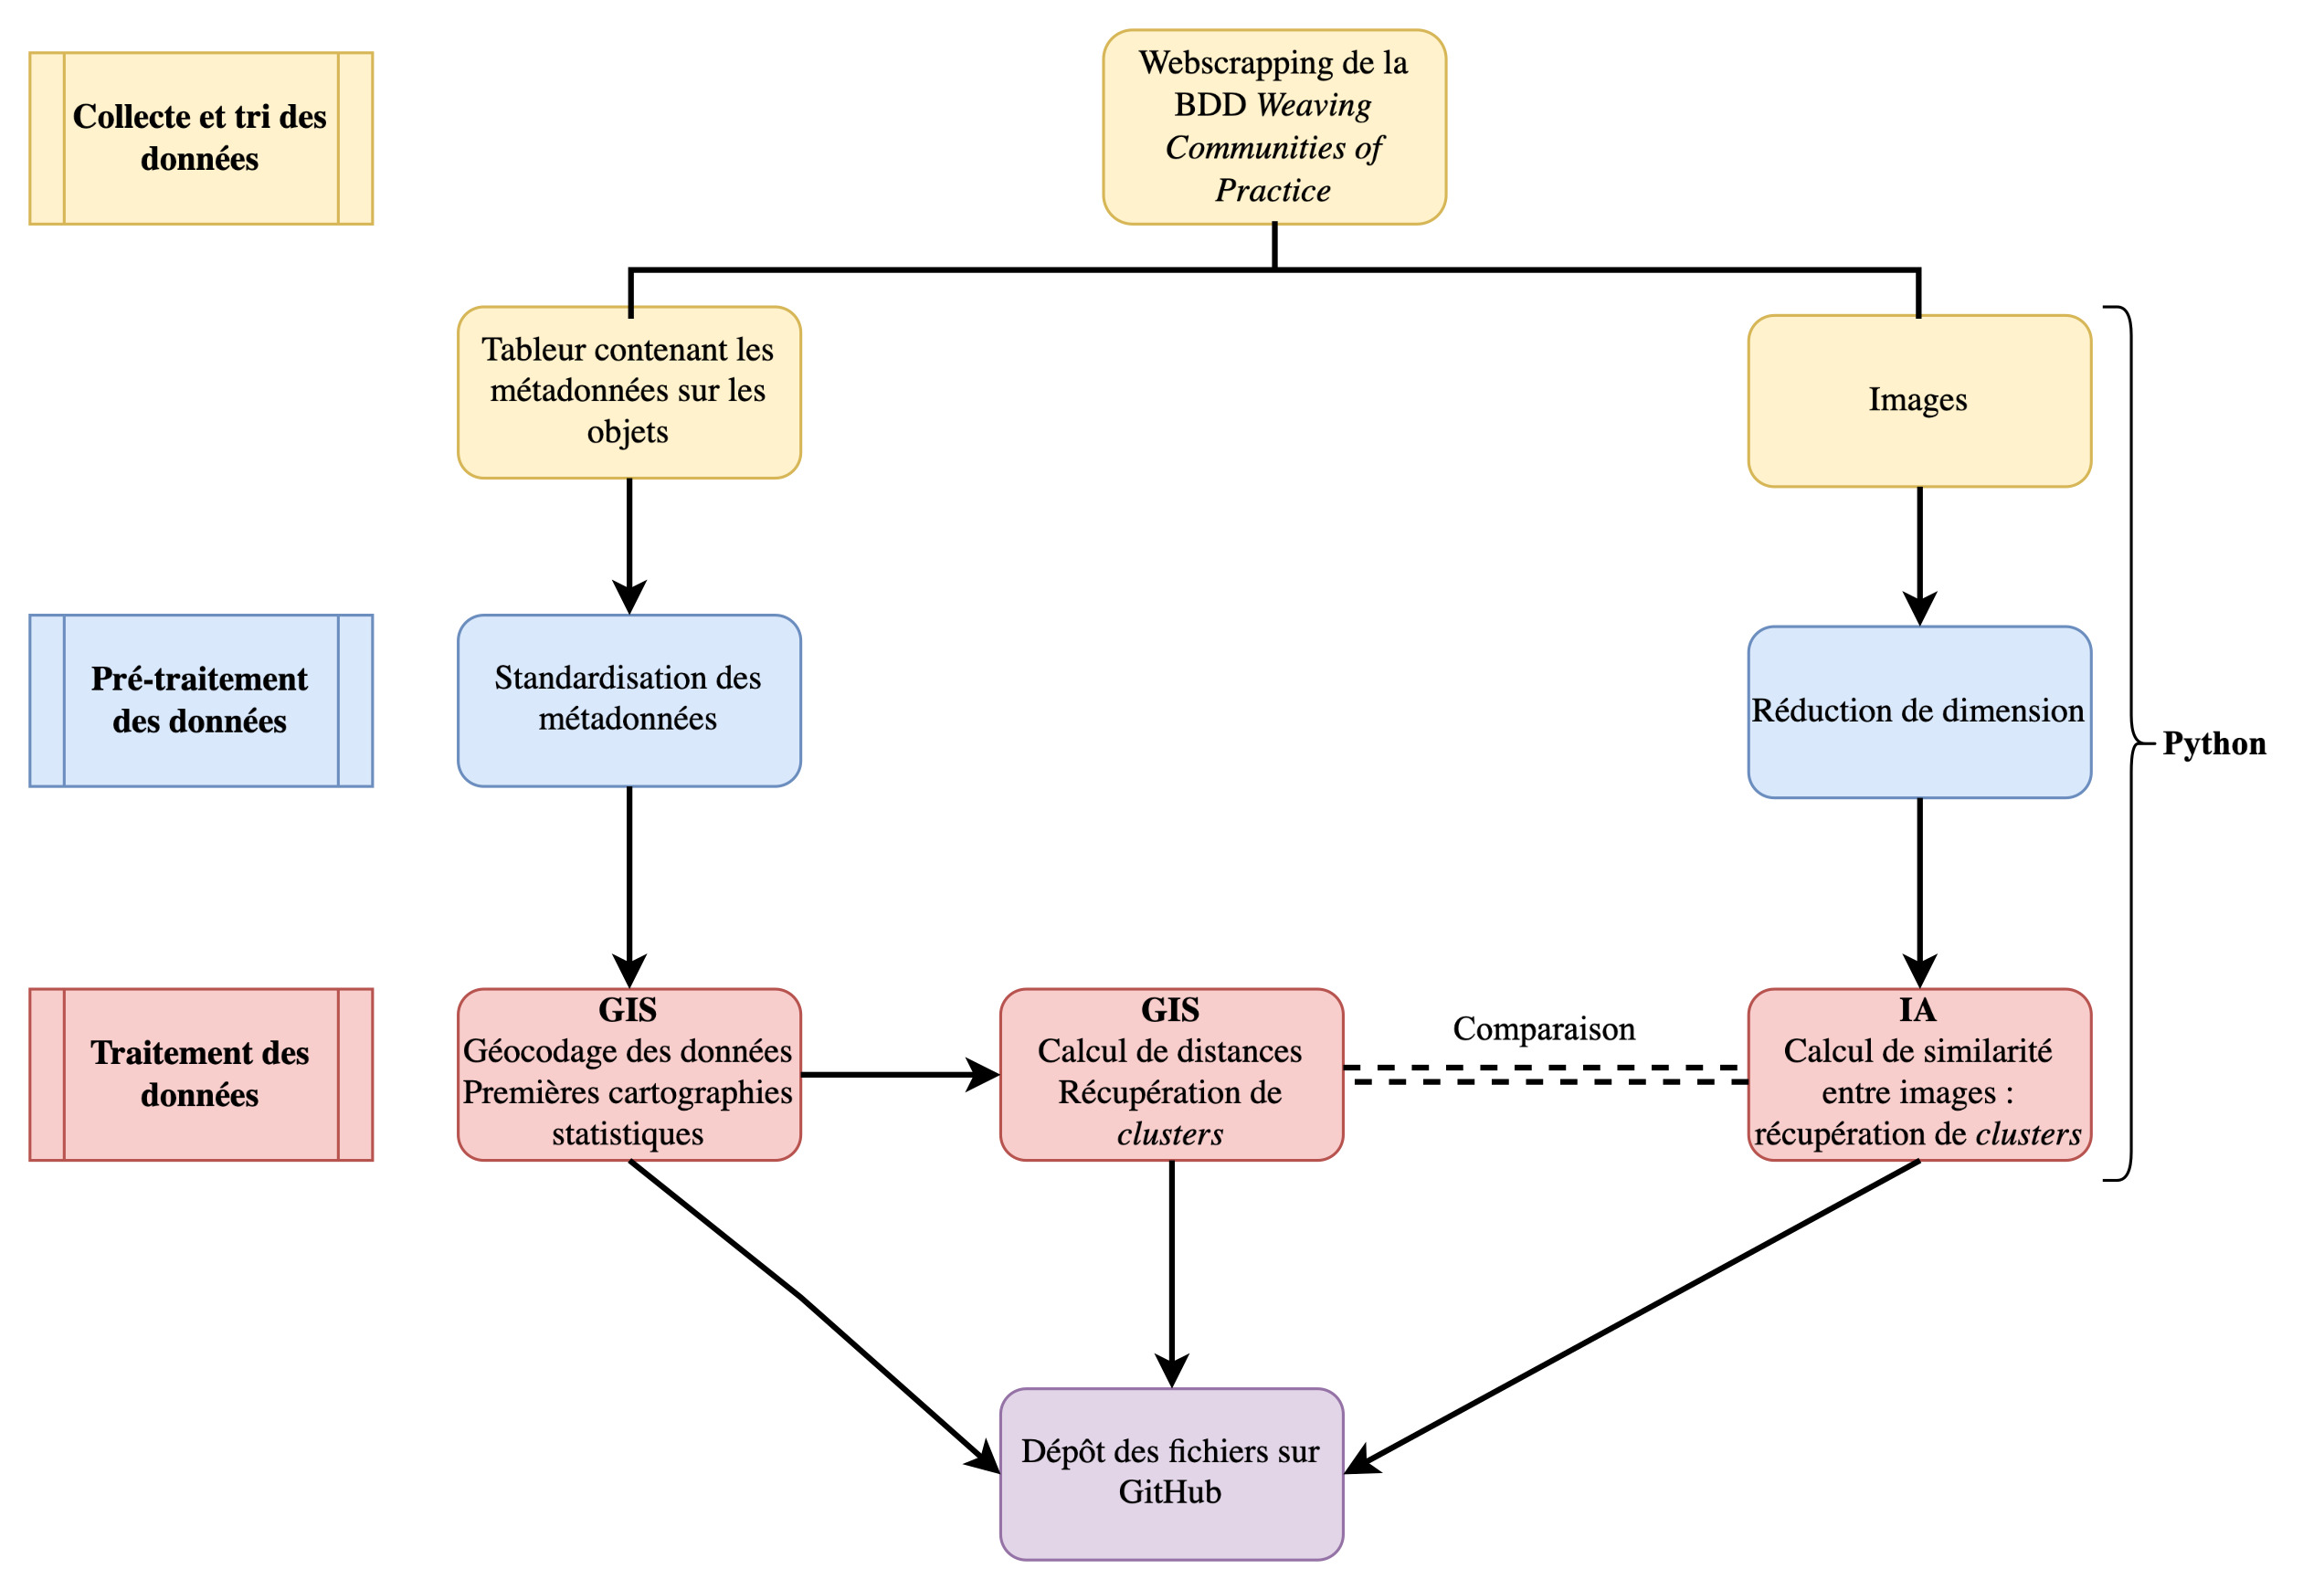
\includegraphics[width=17cm]{../images/pipelineM2.jpg}
           	 \caption{Chaîne de traitement des données menée au cours du mémoire.}
           	 \label{pipeline}
	 \end{center}
  \end{figure}

\chapter{Mieux comprendre les textiles andins par leurs circulation et leurs influences mutuelles ?}
\markboth{}{}

\epigraph{\textquotedblleft In the ancient Andes, art, not necessity, seems to have been the mother of invention.\textquotedblright}{William J. Conklin, 1997, \og Structure as Meaning in Andean Textiles\fg, p.~112.}


\section[Textile et andinité]{Textile et andinité\footnote{Une partie du développement suivant est issu du mémoire de master de Lise Bernard, \textit{De la \textquotedblleft maison-atelier\textquotedblright aux marchés internationaux : ethnographie d'une famille de tisserand\inclusives{e} dans les Andes centrales péruviennes (Ayacucho, Pérou)}.}}

\subsection{Le concept de \og l'andin\fg}

Du nord au sud du Pérou, les habitants revendiquent le textile comme marqueur de l'identité \og andine \fg. 
Les divers champs des sciences sociales qui se consacrent à l'étude des populations vivant dans la Cordillère des Andes sont constamment confrontés à ce concept de \og l'andin \fg. Ce terme englobe en effet plus qu'une zone géographique. Il a  été démocratisé, dans les analyses théoriques,  par John V. Murra, précurseur de l'ethnohistoire des Andes, dans le titre et dans l'introduction de son ouvrage \textit{Formaciones económicas y políticas del mundo andino}\footcite[p.~22]{murraFormacionesEconomicasPoliticas1975}, publié en 1975. Il ne définit pas précisément le terme mais considère qu'il existe une homogénéité des cultures des hautes-terres andines ainsi qu'une continuité entre les hautes civilisations des temps préhispaniques et les cultures contemporaines des Andes. Cette idée persiste dans les disciplines académiques : comme le souligne l'anthropologue Eva Fischer, ce terme mouvant est souvent associé à une persistance du préhispanique sans analyse de l'évolution historique, mettant de côté l'influence de la conquête européenne\footcite[Partie 1, chapitre 1]{fischerUrdiendoTejidoSocial2008}. Par exemple, Gerardo C. Guzmán dans son récent ouvrage sur l'alcool dans les Andes du Sud propose de considérer \og l'andin \fg \:comme un \textit{habitus} qui s'inscrit dans \og l'action même des sujets et [qui est] traversé par les conditionnements sociaux, économiques, politiques et culturels\fg \footnote{\cite[p.~28]{castilloguzmanAlcoholAndinoEmbriaguez2015}. Citation originale : \textquotedblleft \textit{la acción misma de los sujetos y cruzado por condicionamientos sociales, económicos, políticos y culturales}\textquotedblright}. Il ne définit pas non plus ce qu'il entend par ces conditionnements, et ce qu'ils impliquent en matière de pratique ou de distinction par rapport à d'autres parties de la société péruvienne. Alors même qu'il est constamment mobilisé pour définir des pratiques sociales présentes dans les zones de la Cordillères des Andes, notamment les pratiques textiles, ce terme \og d'andin\fg \:est difficile à appréhender.

Pour saisir le terme \og andinité \fg, nous pouvons alors suivre la proposition de l'historien Reinhart Koselleck qui part du postulat que la transformation des mots est un fait social qui permet de comprendre la société actuelle\footcite{koselleckEspacioExperienciaHorizonte1993}. 
Cet auteur présente deux caractéristiques définissant un concept : l'horizon d'attente et le champ d'expériences présentes et passées. 
Les concepts mobilisés ont un contexte historique, ils apparaissent à un moment donné et leur utilisation varie dans le temps. C'est ce que Reinhart Koselleck appelle le \og champ d'expérience \fg\: du concept : \og l'expérience est un passé présent, dont les événements ont été incorporés et peuvent être remémorés \fg\footnote{\cite[p.~338]{koselleckEspacioExperienciaHorizonte1993}}. L'expérience est un champ puisqu'elle cumule les temporalités. 
En outre, le concept ouvre des possibilités de sens que Reinhart Koselleck nomme \og l'attente \fg. Cette attente \og est liée aux personnes, tout en étant impersonnelle, l'attente est aussi dans le présent, c'est le futur fait dans le présent, elle fait référence au pas-encore, à ce qui n'a pas été expérimenté, à ce qui peut seulement être découvert \fg\footnote{Idem.}. L'attente est appelée horizon car elle ouvre une multitude de possibilités, il se passe toujours quelque chose de plus ou en moins de ce qui était prévu. C'est la tension entre la superposition des expériences et des attentes qui génère des possibilités nouvelles. La particularité du concept est d'avoir la capacité de mobiliser les populations pour transformer la société dans le futur. 
Ainsi, \og l'andin \fg \:peut être considéré comme concept (au sens de Koselleck) puisque son champ d'expérience contient, sans distinction, les pratiques des populations préhispaniques et de leurs descendants métisses, réutilisées depuis la colonisation dans les discours politiques et identitaires des acteurs de cette zone géographique\footnote{Nous renvoyons ici aux courants indigénistes puis indianistes qui ont mobilisés l'andinité pour définir les populations autochtones des Andes. L'andinité à aussi été mobilisée plus récemment dans les revendications d'auto-identifications de ces mêmes populations. Pour plus de détails voir : \cite{favreIndigenisme1996}}. Il a pris différents sens à partir de la Conquête et est, encore aujourd'hui, porteur d'un sens identitaire. L'andin est, en effet, un élément important des identités nationales péruvienne et bolivienne, et le textile participe à la diffusion d'une supposée culture andine comme culture nationale. Toutefois, cette mobilisation de l'andin comme concept a tendance à laisser de côté les personnes qu'il désigne, et dans le cas du textile, les groupes qui le produisent créant une dissonance entre population discriminée et pratiques andines valorisées. 

\subsection{Qu'est-ce que l'\og andinité \fg \:textile ?}

Dans le cas du textile, cette association à l'andinité a eu tendance à mettre de côté l'historicité du textile, créant une omission de près de cinq cents ans d'histoire. Cristian Terry, dans sa thèse d'anthropologie, propose plusieurs catégories de textiles \og andins\fg\footcite[p.~154]{terryTisserValeurAu2019}. D'abord, il distingue les textiles produits par des \textit{comuneros}, c'est-à-dire les textiles produits dans des communautés andines contemporaines de manière artisanale et fruit d'un \og savoir-faire textile accumulé historiquement \fg\footnote{Idem.}. Pour compléter l'approche de Terry sur ces textiles \textit{comuneros}, nous pouvons suivre Sophie Desrosiers qui indique que le trait principal de ces textiles des communautés est la création de lés à quatre lisières\footcite[p.~267 et communication personnelle.]{desrosiersTechniquesTissageOntelles2010}. Ces tissus sont principalement produits sur des métiers à la ceinture ou à dossière dont l'existence est attestée depuis 2000 avant J.-C.\footcite[p.~190]{cousinRobeFemmeOrigine2016}. Les techniques de tapisserie sont apparues plus tardivement à l'Horizon Ancien (900 avant J.-C. à 200 avant J.-C.)\footcite[p.~58]{desrosiersMatieresPremieresSavoirs2018}.
Cristian Terry inclut également dans les textiles \og andins\fg\ \:l'ensemble des textiles historiques pré-hispaniques, ainsi que les imitations industrielles contemporaines de ces catégories précédentes.

\begin{wrapfigure}{r}{0.5\textwidth}
    \centering
    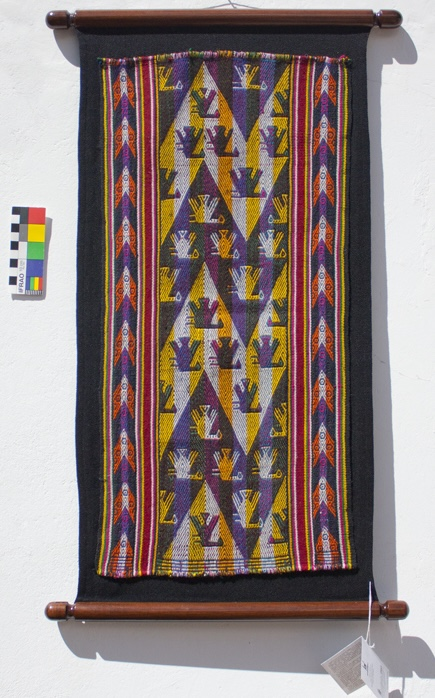
\includegraphics[width=0.5\textwidth]{../images/ASU001.jpg}
    \caption{Textile ethnographique décoratif de la région de Tinkipaya (Bolivie), probablement réalisé sur un métier à la ceinture. \\ Référence dans la base de donnée : ASU001.}
    \label{fig:ASU001}
\end{wrapfigure}

Nous pouvons ajouter certains critères supplémentaires à la proposition de C. Terry : l'imaginaire des textiles andins se compose de tons chauds et intenses, les rouges, oranges et jaunes dominent et les tons pastels sont minoritaires dans les pièces produites, au profit du blanc utilisé pour créer du contraste. Par ailleurs, bien souvent les textiles respectent des codes de symétrie, de géométrie et de répétition de motifs. Cette iconographie peut être en partie rattachée à l'héritage esthétique inca, et plus largement préhispanique, que Catherine J. Allen décrit ainsi : \og Indifférents aux représentations naturalistes, les artistes incas semblent avoir été fascinés par les relations géométriques : avec des croisements, des reflets, des inversions et des répétitions\footnote{\cite[p.~19]{allenWhenUtensilsRevolt1998}. Citation originale : \textquotedblleft \textit{Uninterested in naturalistic representation, Inca artists seem to have been fascinated with geometric relations: with encounters, reflections, inversions and repetitions.}\textquotedblright}.\fg

On retrouve cette esthétique dans les textiles contemporains des Andes avec une prépondérance des représentations géométriques, au détriment des représentations figuratives. Comme l'affirme Eva Fischer, \og les textiles andins se soumettent, avec différents niveaux de complexité, à un régime créatif généré par des symétries, des disymétries et des rythmes\footnote{\cite[p.~226]{fischerUrdiendoTejidoSocial2008}. Citation originale : \textit{\textquotedblleft los textiles andinos se someten, en diferentes grados de complejidad, a un régimen creativo generado por simetrías, asimetrías y ritmos.\textquotedblright}}.\fg \:Même les textiles les plus simples, composés de bandes unies, respectent bien souvent la symétrie avec des rayures alternées symétriquement. Mais la symétrie est aussi présente dans les textiles qui mobilisent des techniques plus complexes. Des motifs figuratifs sont également tissés, notamment la flore et la faune locale mais aussi des motifs issus du répertoire occidental à partir de la Conquête. Ces motifs figuratifs tissés sont souvent géométrisés. Cette géométrisation découle en partie des techniques de tissage et de tapisserie. Comme André Leroi-Gourhan l'explique, le tissage regroupe \og toutes les formes d'assemblage de deux nappes d'éléments parallèles\fg\footcite[p.~81]{leroi-gourhanHommeMatiereEvolution1943}. Dans ce cas, les fils ne peuvent emprunter que deux directions, longitudinale ou transversale, formant un quadrillage. Ce quadrillage contraint la représentation figurative, notamment pour les techniques de tissage les plus simples, créant cette géométrisation. 

L'utilisation de la catégorie \og andine \fg \:pour comprendre le textile génère une forme de standardisation de la vision de cet objet hétérogène. À l'aune des textiles de la base de données, c'est en effet plutôt la diversité qui semble définir le textile andin : diversité des techniques, des motifs, des matériaux et des usages textiles. \\

Le terme \og andin \fg \:pour désigner les textiles provenant des Andes semble donc limiter la compréhension des textiles, les enfermant dans un héritage technique et iconographique immuable depuis cinq siècles. Cette complexité des textiles et de leur histoire mérite un examen plus approfondi. Plutôt que d'envisager les textiles comme une succession régulière de civilisations, nous souhaitons comprendre les influences mutuelles qui apparaissent dans les variations techniques et iconographiques des pièces textiles. Saisir ces influences grâce aux outils numériques nous amènera à nous questionner sur les circulations des savoir-faire et des représentations ainsi que sur les processus de cohabitation, complémentarité et compétition entre les différentes techniques textiles présentes dans un espace aussi vaste que les Andes, du sud de l'Équateur au nord du Chili et de la côte aux piémonts amazoniens.






\section[Les réseaux d'échanges intra et inter-régionaux]{Les réseaux d'échanges intra et inter-régionaux : la circulation physique des textiles et de leurs matériaux}

La circulation physique des textiles et de leurs matériaux est difficile à saisir. Comme nous l'avons déjà souligné, les conditions de conservation textiles ne permettent que très rarement d'avoir accès à des restes de la culture textile dans les hautes-terres et cette répartition lacunaire des textiles archéologiques sur le territoire complique la compréhension de leurs parcours. 

\subsection{La circulation des textiles et des matériaux à la période pré-hispanique}

L'analyse des circulations de matériaux sur le territoire andin porte principalement sur les matériaux rares et exotiques qui ont circulé intensément sur le temps long et sur de longues distances. Par exemple, Anne-Marie Hocquenghem retrace les routes d'échanges du \textit{spondylus}, coquillage provenant de l'Équateur, de l'Horizon Ancien à l'Horizon Tardif. Elle montre que les routes sont multiples et évoluent avec le temps. Or, contrairement au \textit{spondylus}, les textiles ne sont pas des objets rares et exotiques dans la région. Le textile était produit dans toute la zone et ce depuis que l'on y retrace une présence humaine, notamment pour les raisons pragmatiques que souligne John Murra : \og tous les peuples andins portaient des vêtements pour la simple raison qu'il faisait froid, et l'archéologie nous dit qu'ils le faisaient bien avant les Incas\fg\footnote{\cite[p.~716]{murraClothItsFunctions1962}. Citation originale : \textquotedblleft \textit{All Andean peoples wore clothes for the simple reason that it was cold, and archeology tells us they did so long before the Incas.}\textquotedblright}. 

Cette omniprésence du textile dans la zone andine s'accompagne d'une circulation des fibres textiles. Avant l'arrivée des espagnols et l'introduction des fibres ovines, le coton et la laine des différents camélidés andins (vigogne, alpaga, lama et guanaco) servaient de fibres principales pour la production textile. Ces derniers sont domestiqués dans les hautes-terres au cinquième millénaire avant notre ère\footcite[p.~12]{boissiereAtlasAmeriquePrecolombienne2022}. Sur la côte, la culture du coton est attestée dans le nord du Pérou dès le quatrième millénaire avant notre ère\footcite[p.~13]{boissiereAtlasAmeriquePrecolombienne2022}. Ces deux fibres étaient dépendantes de conditions écologiques précises et donc réparties dans des zones différentes. Cette répartition géographique des fibres favorise leur circulation, facilitée \og par des distances réduites dues à des changements d'altitude rapides et/ou des politiques expansionnistes des sociétés des hautes-terres\fg\footcite[p.~52]{desrosiersMatieresPremieresSavoirs2018}, d'autant plus que les fibres ont des caractéristiques différentes. Le coton, apprécié pour sa résistance, constitue la chaîne de certains tissus des hautes-terres alors que la laine de camélidés, accrochant mieux les teintures, est plutôt utilisée sur la côte pour former les décors\footnote{Idem.}.

\begin{figure}[!ht]
        \begin{center}
        		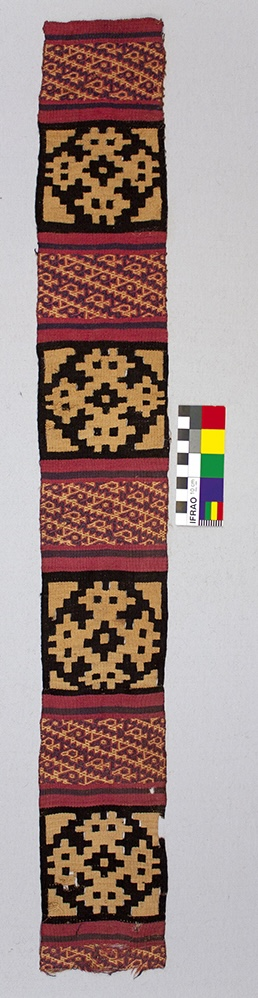
\includegraphics[width=4.2cm, angle=-90]{../images/BML021_IMG_3319.jpg}
	\end{center}
    \caption{Fragment de tapisserie côtière (Chancay, côte centrale) de la période Intermédiaire Tardive (1000-1470). Trame en coton et laine de camélidé, chaîne en coton. \\ Référence dans la base de donnée :  BML021.}     
    \label{fig:BML021}
\end{figure}

\noindent Des matériaux plus rares constituent également les textiles, notamment pour les décors. Ainsi, les coquillages, les plumes, notamment amazoniennes, les perles en pierres, les plaquettes de métal illustrent \og le recours à toutes les zones géographiques pour créer des \oe{}uvres spectaculaires et chargées de signification\footnote{Idem.}.\fg \:Les pièces composées de plusieurs matériaux différents illustrent la maîtrise des artisans à mobiliser des savoir-faire variés. La présence de cette multiplicité de matériaux, de laine de camélidés sur la côte et de coton dans les Andes, atteste d'une circulation. Toutefois, les conditions de transport des matériaux ne sont pas toujours connues : les fibres ont pu être transportées brutes, filées et même tissées.\\

La circulation physique des matériaux prend différentes formes dans les Andes. Sur le territoire andin, de multiples populations se sont côtoyées organisées en différentes groupes politiques, de la société nomade à l'Empire. Ces différentes configurations sociales impliquent des échanges différenciés et leur compréhension permet de saisir la manière dont les textiles ont pu circuler dans les Andes.

La domestication des camélidés au cinquième millénaire avant notre ère favorise la constitution de sociétés pastorales dont les économies reposent sur cette ressource. Dans le bassin Jauja-Huancayo (Andes centrales péruviennes), les sociétés antérieures au sixième siècle dépendent des lamas et des alpagas qui représentent 50\% de leur subsistance\footcite[p.~188]{browmanPastoralNomadismAndes1974}. 
Le reste de leur approvisionnement repose sur des productions secondaires, l'horticulture ou le commerce réalisé avec des caravanes de lamas qui permettent d'avoir une stabilité économique et politique grâce à \og  des échanges marchands raisonnables, tant sur le plan idéologique que matériel \fg\footnote{Ibid, p.~191. Citation originale : \textquotedblleft \textit{a reasonable amount of mercantile exchange, both on the ideological and on the material level.}\textquotedblright}. Ces échanges marchands comprenaient possiblement des textiles. David L. Browman qui a étudié les sociétés pastorales andines en croisant les données archéologiques, ethnohistoriques et ethnographiques relève que les routes et les biens échangés ont peu changé au fil du temps\footcite[p.~195]{browmanPastoralNomadismAndes1974}, il ajoute que les personnes qui circulent avec ces caravanes dans les années 1970 \og partent généralement de leur propre communauté avec des textiles, de la viande séchée, de la graisse, des peaux, de la laine, du chuño\footnote{Le chuño désigne les pommes de terre déshydratées par le gel et le soleil, encore consommées dans les Andes à notre époque.} et d'autres tubercules\fg\footnote{Idem. Citation originale : \textquotedblleft \textit{The drovers generally start out from their own community with textiles, dried meat, fat, hides, wool, and chuño and other tuber products.}\textquotedblright}. 
L'économie des sociétés pastorales repose en partie sur la laine qui est une de leurs ressources principales et que les commerçants peuvent ensuite échanger. Le commerce et la mobilité semblent donc d'une grande importance, notamment pour certaines populations des hautes-terres qui habitent des environnements de haute altitude et qui souhaitent accéder aux ressources d'écozones variées\footcite[p.~389]{nielsenCirculatingObjectsConstitution2013}. Axel Nielsen dans son analyse de la circulation des objets dans les Andes souligne lui aussi l'importance des caravanes de camélidés comme principale source de mobilité :  
\begin{citer}
	[Les] preuves d'une circulation inter-régionale des marchandises remontent à la période archaïque (8000-1500 av. J.-C.) et semblent s'accroître à la fin de la période archaïque et au début de la période formative (1500-500 av. J.-C.), lorsque la domestication des lamas a amélioré les capacités des premiers éleveurs-chasseurs-horticulteurs pour transporter des charges volumineuses sur de grandes distances\footnote{Ibid., p.~400. Citation originale : \textquotedblleft \textit{evidence of interregional circulation of goods dates back to the archaic period (8000-1500 BC) and seems to increase during the late archaic and early Formative periods (1500-500 BC), when the domestication of llamas enhanced the capacity of early pastoralists-hunters-horticulturalists to transport bulky loads over great distances.}\textquotedblright}.
	\end{citer}

\noindent Son étude porte plus précisément sur la circulation inter-régionale dans les Andes Sud (nord-est de l'Argentine, nord du Chili et sud-ouest de la Bolivie) entre 500  av. J.-C. et 1550 ap. J.-C., sur toute la largeur des Andes. Entre 500  av. J.-C. et 500 ap. J.-C., il distingue les échanges qui ont lieu entre les éleveurs de lamas et les fermiers locaux du commerce par les \og pastoralistes spécialisés \fg. Ces derniers intégraient l'échange comme activité centrale de leur mode de vie puisqu'ils n'étaient pas soumis aux mêmes contraintes sociétales. Sur toute la période étudiée, Axel Nielsen relève deux sphères de circulation différenciée. D'une part, une sphère restreinte aux psychotropes, aux armes qui servent d'emblèmes politiques, aux textiles fins, aux couvre-chefs élaborés et aux ornements en métal. D'autre part, une sphère d'échange non restreinte au sein de laquelle circulent céramiques, objets lithiques, bois pour les flèches, plumes, textiles moins sophistiqués, coquillages, feuilles de coca, maïs, et biens périssables\footnote{Ibid., p.~414}. Michelle Young développe la même observation à propos des échanges entre les Andes centrales et la côte à l'Horizon Ancien (de 800  av. J.-C. à 200  av. J.-C.), elle reprend les produits proposés par David L. Browman mais ajoute également les produits contre lesquels ils seraient échangés ainsi que différentes étapes des caravanes : 

\begin{citer}
	Ils auraient transporté tout ce qui pouvait être échangé, par exemple des textiles ; des produits des camélidés, tels que le char'ki [viande séchée], la graisse, le cuir et la laine ; chuño et autres tubercules. Ces produits auraient pu être apportés de leurs propres communautés afin de les échanger avec des produits agricoles, céramiques, métaux, etc., provenant d'autres colonies de montagnes situées le long de la route, ou éventuellement pour les échanger avec des objets d'autres communautés.\footnote{\cite[p.~28]{youngMontanaMarIntercambio2017}. Citation originale : \textquotedblleft \textit{habrían transportado cualquier cosa que pudiera ser objeto de intercambio, por ejemplo, textiles; productos de camélidos, como char'ki, grasa, cuero y lana; chuño y otros productos de tubérculos. Estos productos podrían haber sido traídos de su propia comunidad con el fin de intercambiarlos con los productos agrícolas, de cerámica, de metal, etc., de otros asentamientos de la sierra ubicados a lo largo del camino, o eventualmente para intercambiarlos con objetos de otras regiones.}\textquotedblright}.
\end{citer}

L'archéologie nous confirme donc que les sociétés pastorales nomades échangent amplement, y compris du textile, par le biais de caravanes de lamas suivant des routes qui couvrent toute la largeur des Andes. Ces contacts entre sociétés éloignées prenaient différentes formes, constants ou intermittents, directs ou indirects, selon différentes régularités et intensités d'échanges. \\


Tout comme dans les sociétés nomades et commerçantes, les sociétés sédentarisées et hiérarchisées échangeaient des textiles. Ces circulations sont particulièrement visibles dans les études sur les empires et leur expansion, notamment l'empire Inca pour lequel les données abondent. L'expansionnisme de certaines civilisations andines implique des changements démographiques importants et la mise en contact de cultures éloignées. Ainsi, Axel Nielsen, dans son étude sur les routes dans les Andes Sud, relève que l'influence Tiwanaku dans cette zone au cours de l'Horizon Moyen s'observe dans la fréquence de biens lointains : \og Les plus célèbres parmi ces produits sont les articles de style Tiwanaku, tels que les gobelets à bec (keros), les accessoires à priser et les textiles\fg\footnote{\cite[p.~401]{nielsenCirculatingObjectsConstitution2013}. Citation originale : \textquotedblleft \textit{Most famous among these goods are Tiwanaku-style items, such as beakers (keros), snuffing paraphernalia, and textiles.}\textquotedblright}. Les textiles sont notamment intégrés aux contextes funéraires, utilisés conjointement avec des biens de style local. 

\begin{figure}[!ht]
       \begin{center}
        		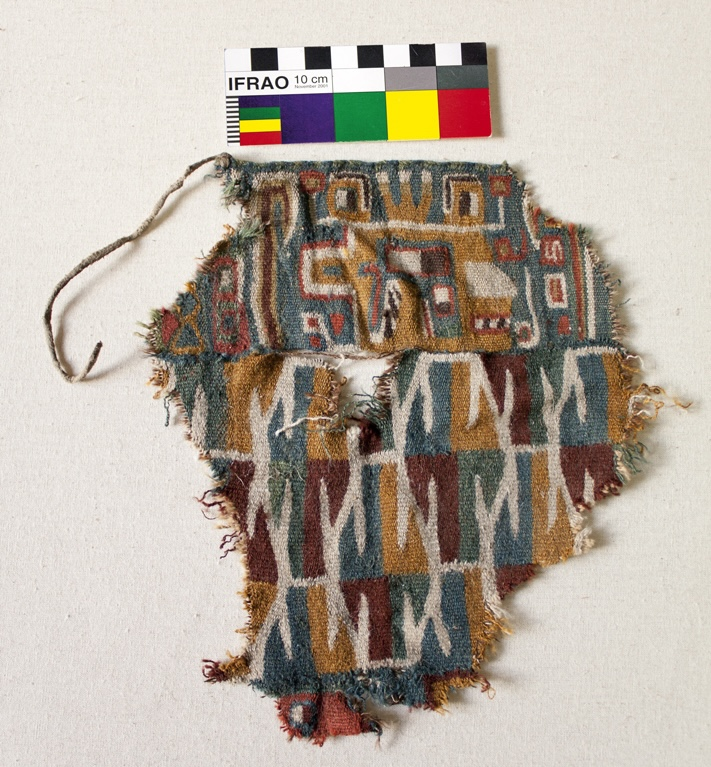
\includegraphics[width=11cm]{../images/MNA037_IMG_2829.jpg}
	\end{center}
    \caption{Fragment de \textit{reps} de trame de style Tiwanaku de l'Horizon Moyen (600-1000). \\ Référence dans la base de donnée : MNA037.}     
    \label{fig:MNA037}
\end{figure}

Le cas de la civilisation Tiwanaku est particulièrement intéressant puisque la coexistence de biens de différents styles concordent avec un modèle d'expansion par  \og un commerce intensifié mais décentralisé, multidirectionnel et conduit localement\fg \footnote{Ibid., p.~405. Citation originale : \textquotedblleft  \textit{intensified, but decentralized, multidirectional, and locally driven trade.}\textquotedblright}. 

L'empire Inca est la société préhispanique la plus dotée en sources textuelles et, conséquemment, la plus étudiée. Les chroniqueurs s'accordent sur le rôle central du textile en son sein. Les habitants de l'empire ont pour obligation de tisser pour l'élite politique et religieuse. Les fibres sont fournies par l'État et apportées aux femmes pour qu'elles les filent et les tissent ou bien produites par les populations locales sur des champs appartenant à l'État\footcite[p.~715-716]{murraClothItsFunctions1962}. Les témoignages des conquérants espagnols concordent sur l'existence de grands entrepôts du nord au sud du Pérou dont beaucoup contenaient de la laine, du coton, des tissus et des vêtements comptabilisés par des agents étatiques\footnote{Ibid., p.~721}. La royauté offre également du textile à ses vassaux dans une logique de réciprocité. Comme l'indique John Murra, les chroniqueurs sont surpris d'observer que, contrairement aux pratiques européennes, \og dans la zone andine, l'artefact le plus prestigieux mais aussi le plus utile dans les relations de pouvoir était le tissu\fg\footnote{Ibid., p.~717. Citation originale : \textquotedblleft \textit{in the Andean area, the artifact of greatest prestige and thus the most useful in power relations was cloth.}\textquotedblright}. 

\begin{figure}[!h]
	\begin{minipage}[c]{.5\linewidth}
        		\begin{center}
        			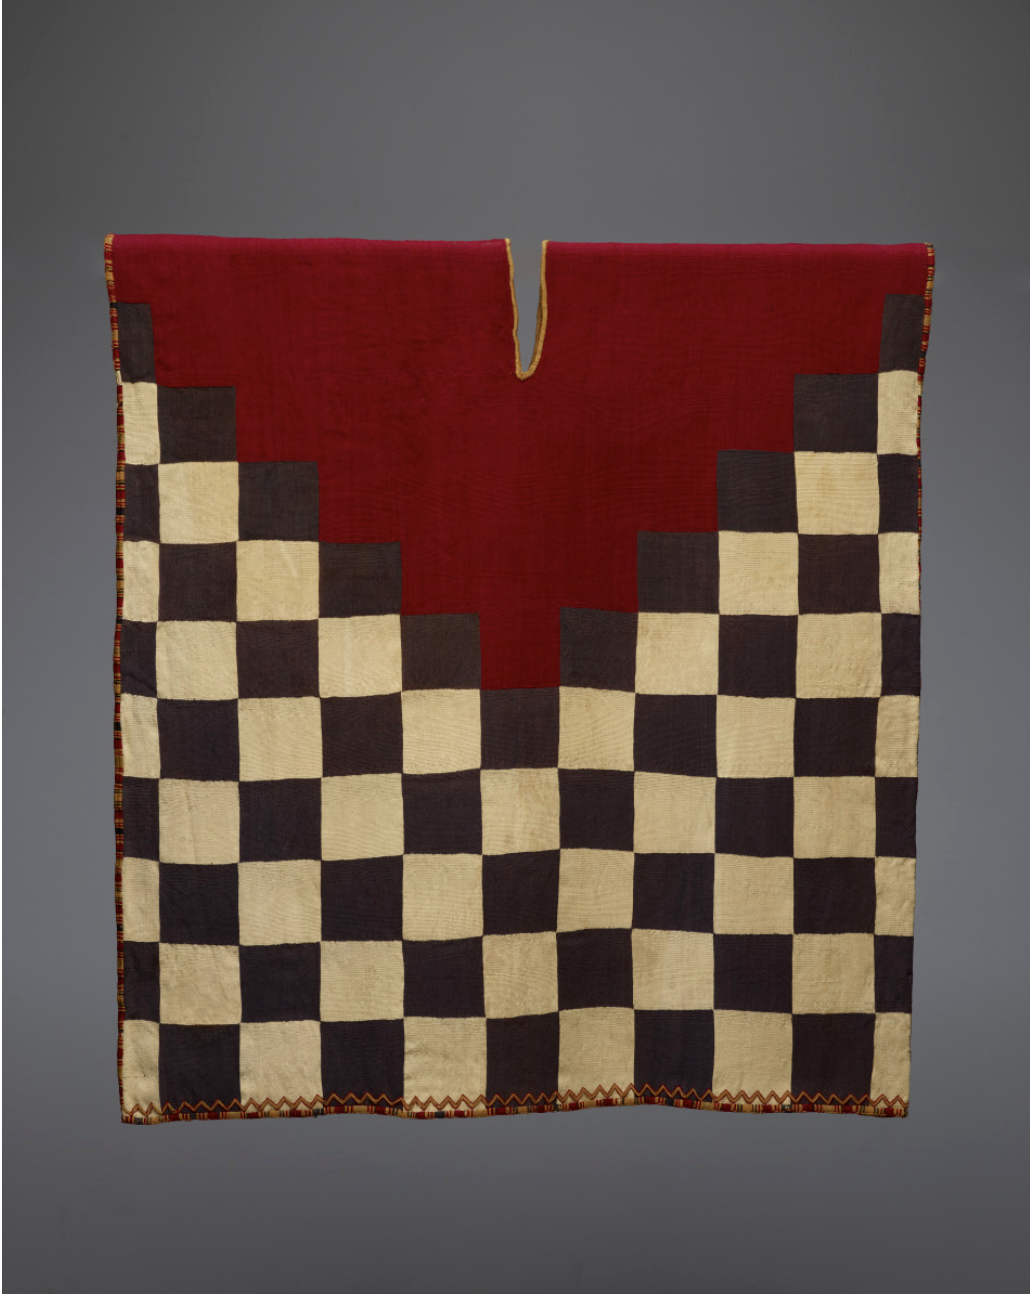
\includegraphics[width=7cm]{../images/unku_DMA.png}
        		\end{center}
	\end{minipage}
	\begin{minipage}[c]{.5\linewidth}
        		\begin{center}
			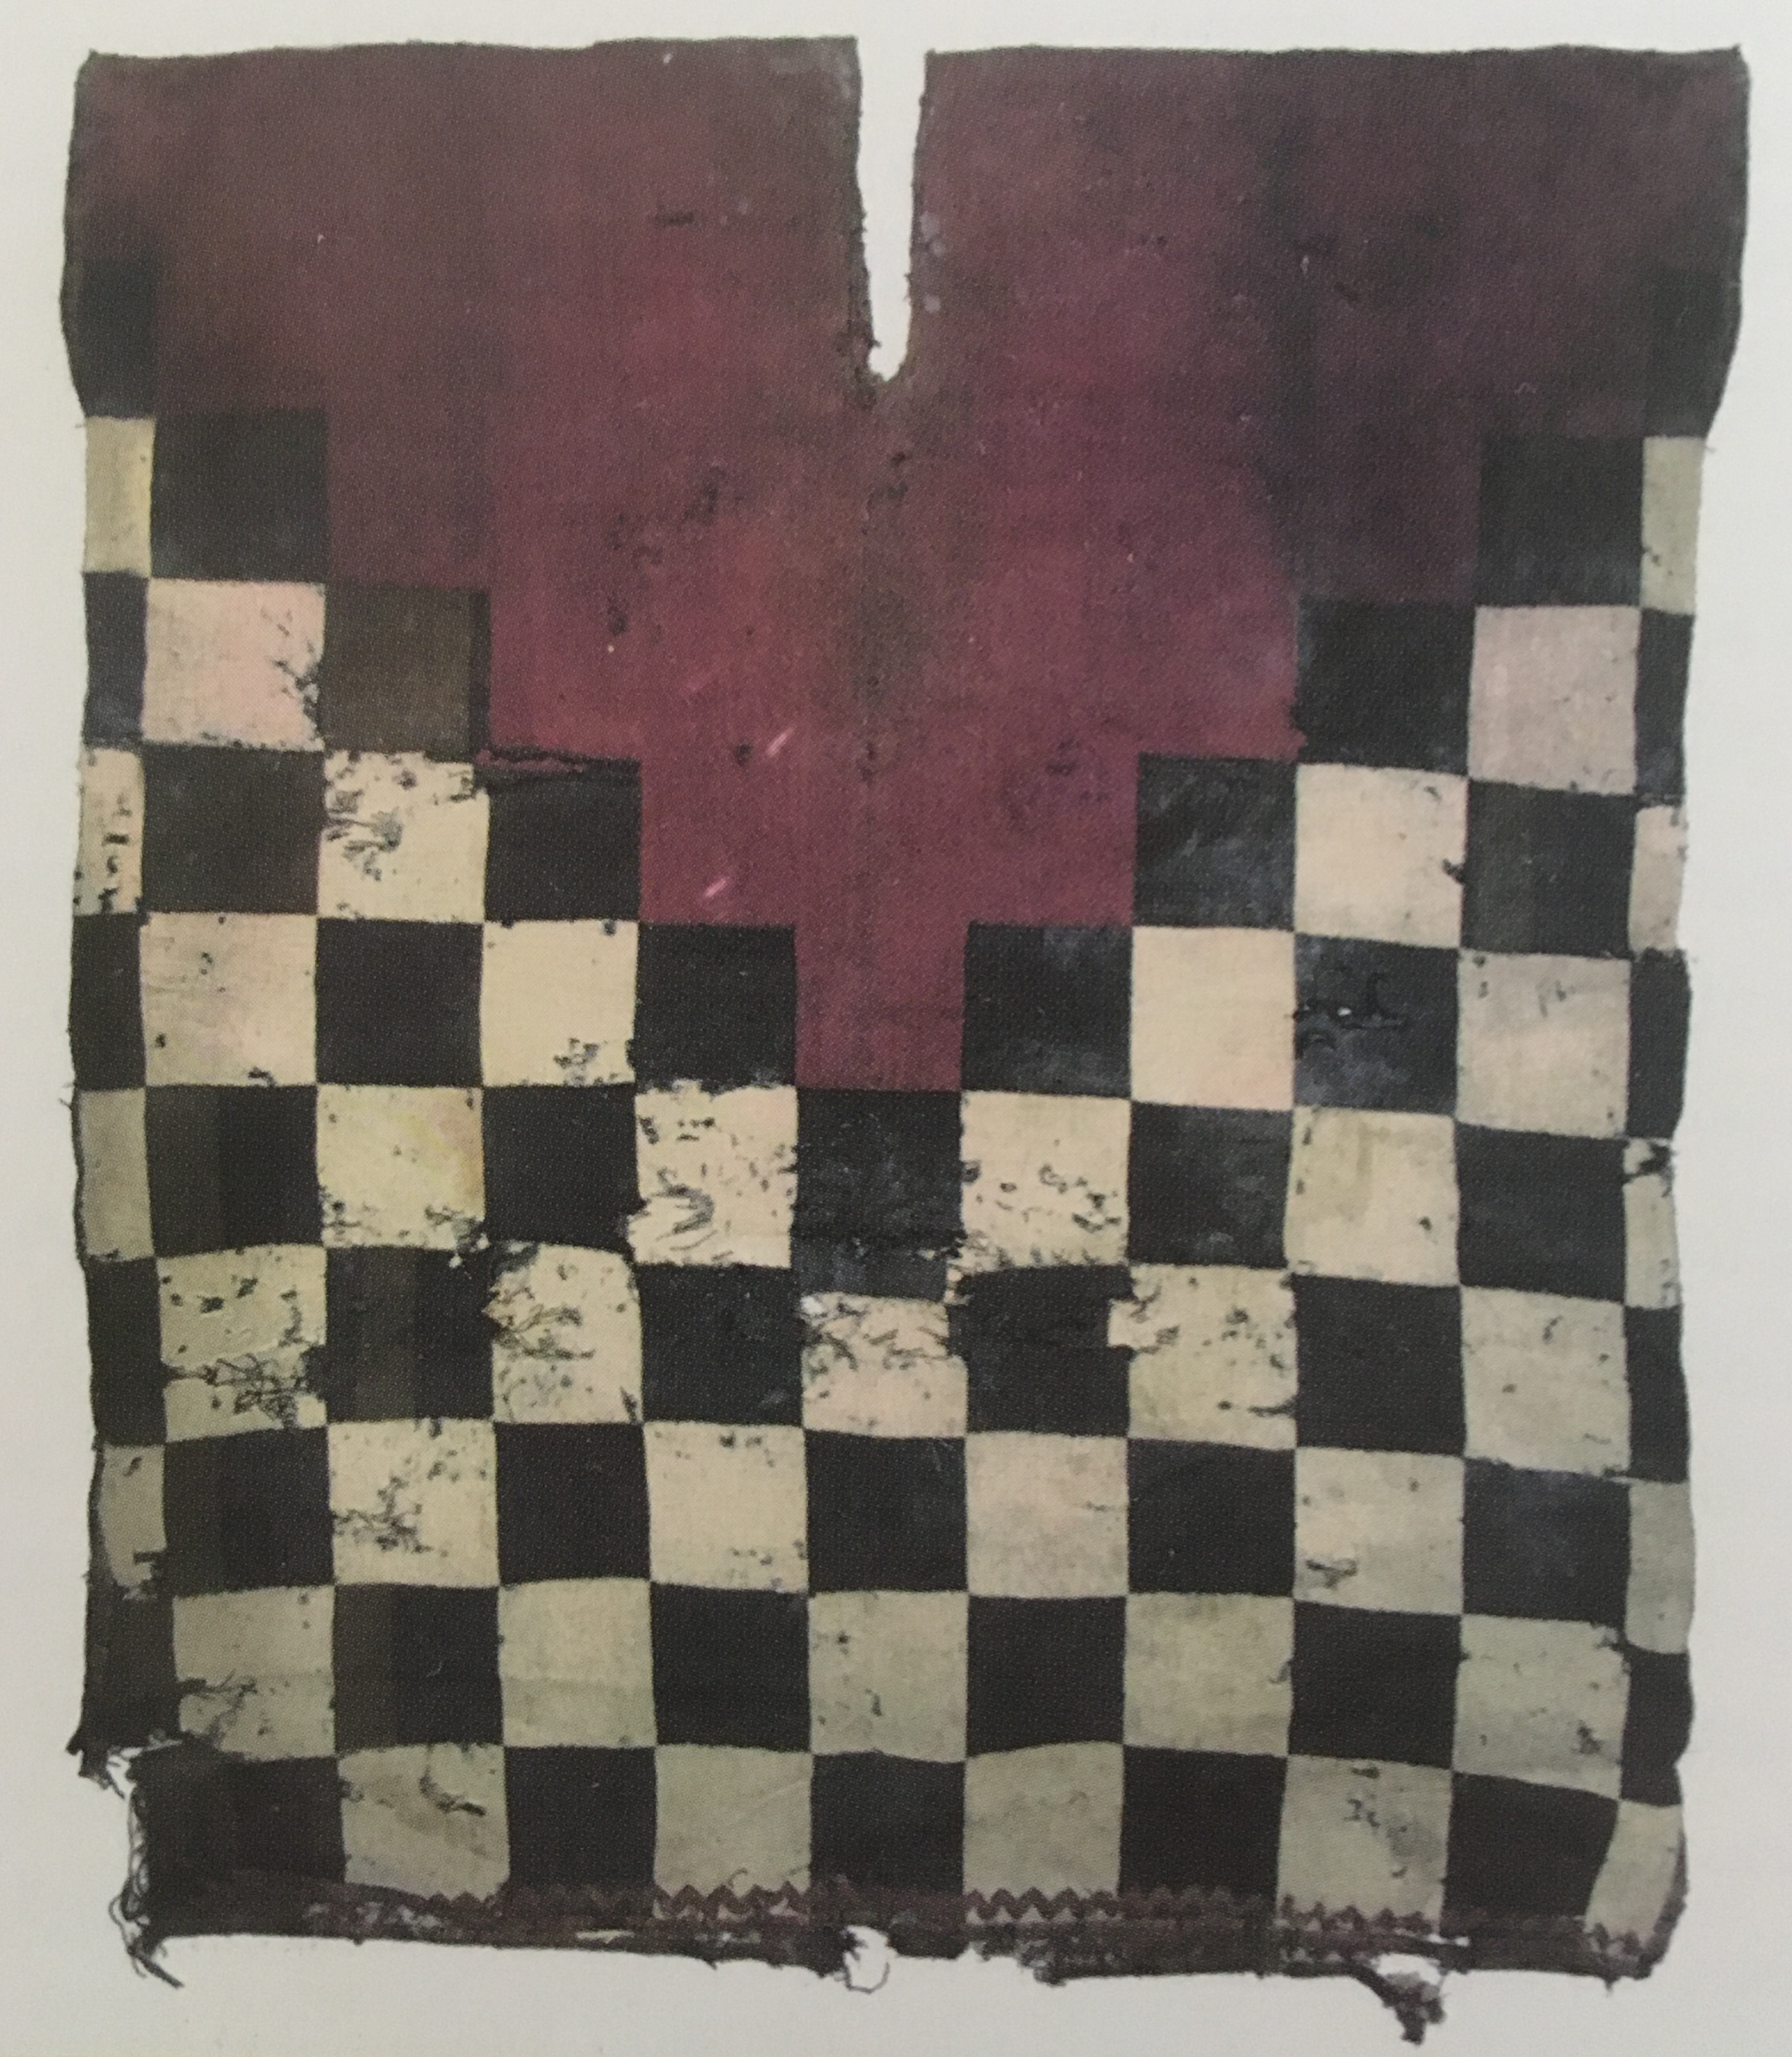
\includegraphics[width=8cm]{../images/unku_volcan.JPG}
        		\end{center}
	\end{minipage}
	\caption[Tunique inca ou \textit{unku} standardisée.]{Tunique inca ou \textit{unku} standardisée. La seconde a été découverte sur le Nevado Chuscha (Argentine) portée par une momie.\\ Sources : respectivement, collections en ligne du Dallas Museum of Arts, The Eugene and Margaret McDermott Art Fund, Inc. in honor of Carol Robbins (\url{https://www.dma.org/art/collection/object/5122425}) et C. Abal de Russo, \textit{Arte textil incaico en ofrendatorios de la alta cordillera andina}, 2010, p.~394.}
	\label{fig:damier}
\end{figure}

Les pièces incas les plus fines sont particulièrement reconnaissables car très standardisées\footnote{Voir : \cite[p.~60]{nilesArtistEmpireInca1994} et \cite[p.~118]{ramosTejidosSociedadColonial2010}}, contrairement aux cultures préincas. Ces pièces similaires attestent de la circulation des textiles. Par exemple, à ce jour, une dizaine de tuniques en damier noir et blanc avec un empiècement rouge ont été découvertes sur tout le territoire de l'empire Inca\footcite[p.395]{abalderussoArteTextilIncaico2010}. Elles étaient probablement destinées à des membres de l'élite inca\footcite[p.54]{nilesArtistEmpireInca1994}, d'où l'exemplaire trouvé dans la tombe d'une enfant sacrifiée au sommet d'un volcan argentin, dans une zone reculée de l'empire, entourée uniquement d'objets d'une grande finesse\footcite[p.260]{abalderussoArteTextilIncaico2010}.

Cette circulation des textiles pour les périodes inca et coloniale repose aussi sur l'organisation des sociétés en \og archipels verticaux \fg\footcite[p.~60]{murraControlVerticalMaximo1975}. John Murra explique que les sociétés andines de cette période ont eu tendance à contrôler des territoires au sein de différents étages écologiques pour assurer leur économie grâce à l'accès aux ressources de ces niveaux. Leurs économies reposent alors sur des produits des zones en altitude, autour de 4000 mètres, et des côtes, au niveau de la mer, reliées entre elles par des échanges de biens.

\subsection{L'élargissement des échanges à la période coloniale}

\begin{figure}[!ht]
       \begin{center}
        		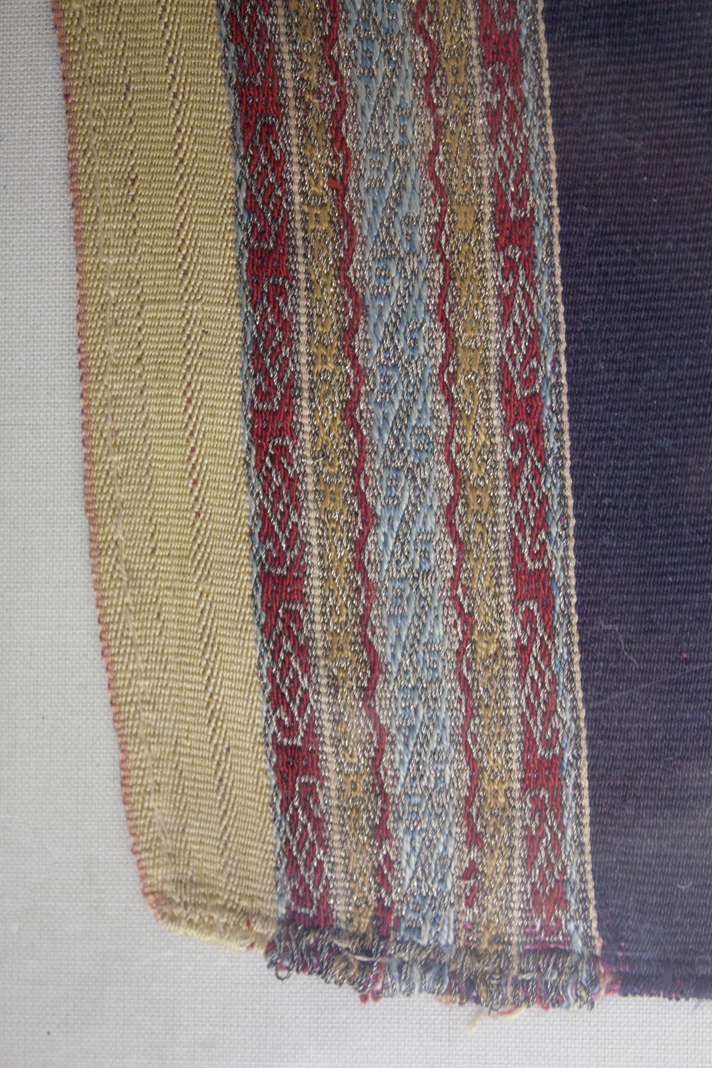
\includegraphics[width=10cm]{../images/MSF070_IMG_6250.jpg}
	\end{center}
    \caption{Bord d'un textile colonial en \textit{reps} de chaîne composé de fils de camélidés (fils de couleurs), fils de coton (blanc) et fils de métal avec une âme de coton. \\ Référence dans la base de donnée : MSF070.}
    \label{fig:MSF070}
\end{figure}

La colonisation introduit de nouveaux modes de circulation des fibres et des textiles à une échelle internationale. Comme le souligne Vera-Simone Schultz pour le monde médiéval islamique, \og en tant qu'objets incassables, facilement transportables, légers et de grande valeur, les textiles constituaient un domaine privilégié pour l'élaboration de langages artistiques interculturels \fg \footnote{\cite[p.~96]{schulzCrossroadsClothTextile2016}. Citation originale : \textquotedblleft \textit{As unbreakable, easily portable, lightweight items of high value, textiles were a privileged domain for the elaboration of cross-cultural artistic languages.}\textquotedblright}. Le même phénomène s'observe pour la zone andine : la colonisation est une période d'échanges intensifs, les textiles étant le bien le plus importé depuis la métropole espagnole pour l'usage personnel des colons ou à visée commerciale\footcite[p.~33]{phippsIberianGlobe2013}. Les manifestes des flottes espagnoles indiquent qu'à la fin du \siecle{xvi}  \og plus de six millions de réaux de tissus et de vêtements arrivaient chaque année d'Espagne\fg\footnote{Ibid., p.~34. Citation originale : \textquotedblleft \textit{more than six million reals' worth of cloth and clothing were arriving from Spanish each year}\textquotedblright}. Ces échanges sont d'autant plus importants que la société coloniale s'enrichit amplement des exploitations minières et est donc en mesure de participer au commerce international. Toutefois, l'arrivée des colons modifie peu l'organisation de la production locale, puisque ceux-ci, tout comme les Incas, reconnaissent la finesse du travail des artisans et requièrent des populations qu'ils produisent des textiles\footcite[p.~52]{nilesArtistEmpireInca1994}. Le métissage des pratiques textiles s'observe notamment dans les matériaux utilisés. Avec l'ouverture de routes commerciales maritimes reliant l'Asie à l'Europe en passant par les Amériques, la soie, le lin, la laine de moutons et les fils métalliques intègrent les textiles andins\footnote{Ibid., p.~51}.
L'arrivée des matériaux dépend des régulations coloniales. Ainsi, la soie chinoise est d'abord interdite pour ne pas faire concurrence aux biens en soie espagnole mais est finalement autorisée face à la demande conséquente de la société coloniale\footcite[p.~34]{phippsIberianGlobe2013}. \\

L'analyse des textiles andins nous plonge donc dans une complexité d'échanges de biens reposant sur de multiples circulations physiques. Les textiles et les sources textuelles nous apportent une grande quantité d'indices matériels de cette circulation. La variété considérable d'indices des échanges textiles, à travers le commerce ou les aires d'influence de sociétés, rend difficile la saisie intégrale de ces échanges qui pourtant mériteraient une vision globale. Les outils numériques apportent cette capacité à prendre un point de vue surplombant sur ces échanges et à saisir la complexité des circulations des textiles andins. Michelle Young, dans son analyse sur les échanges entre les hautes-terres centre-sud et la côte pendant l'Horizon Ancien, distingue les échanges économiques en tant qu'échange de biens entre deux groupes de population, de l'influence culturelle qui implique qu'un groupe adopte les idées et le style d'un autre groupe\footcite[p.~10]{youngMontanaMarIntercambio2017}. Or, l'influence culturelle est centrale dans les évolutions des textiles andins et ceux-ci ne peuvent se comprendre qu'à l'aune de ces influences.



\section[Influences textiles]{Les influences textiles par la circulation des groupes sociaux ou entre différents médiums}

\subsection{Les processus d'imitations préhispaniques}

Les pratiques textiles en termes de matériaux, d'iconographies ou de techniques sont largement influencées par les contacts entre sociétés. Dans le cas andin, ces influences sont particulièrement détectables au cours des \og Horizons \fg, périodes archéologiques marquées par l'expansion d'empires.  
\begin{figure}[!ht]
       \begin{center}
        		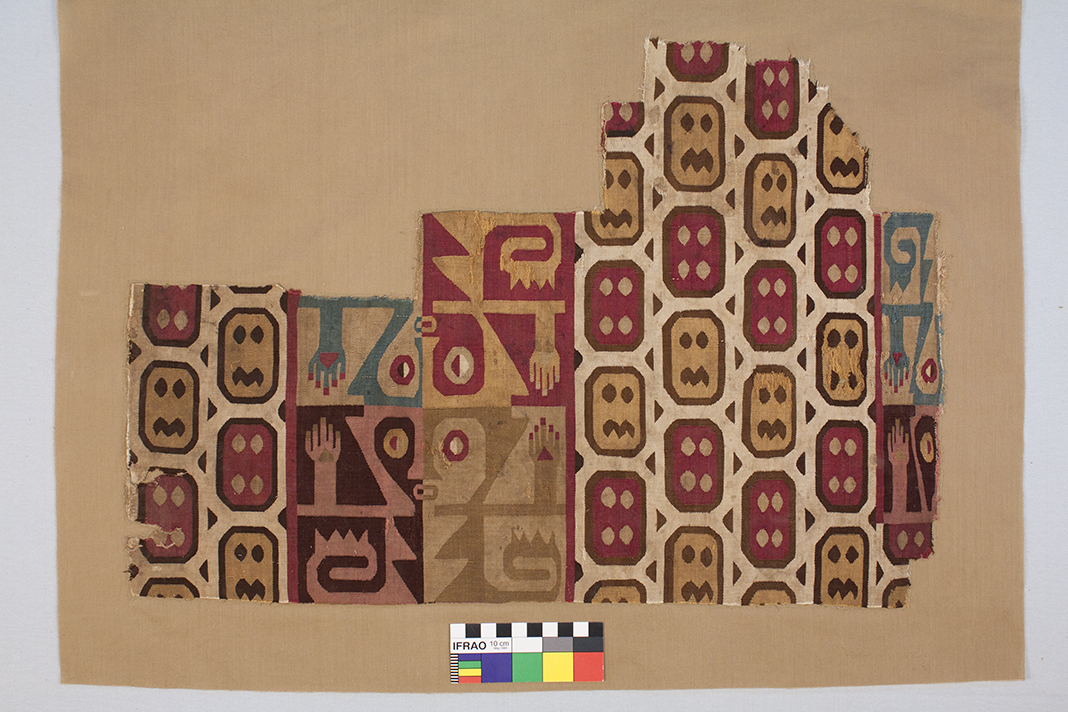
\includegraphics[width=10cm]{../images/BML009_IMG_3240.jpg}
	\end{center}
    \caption{Fragment de tapisserie de style Huari découverte sur la côte sud du Pérou.\\ Référence dans la base de donnée : BML009.}
    \label{fig:BML009}
\end{figure}
L'expansion de l'empire Huari modifie ainsi le mode de vie des populations nomades des Andes centrales péruviennes : les habitants construisent des zones de stockage ainsi que des centres administratifs. Le style Huari s'impose par l'expansion coloniale au cours de l'Horizon Moyen. Dans la région de Jauja-Huancayo, étudiée par David L. Browman, les découvertes archéologiques indiquent une hiérarchisation des sociétés locales sous l'influence des colons, avec l'apparition d'artisans spécialisés qui intègrent l'iconographie Huari\footcite[p.~191]{browmanPastoralNomadismAndes1974}. 
Au cours de l'Horizon Récent, caractérisé par l'expansion de l'empire Inca, ces influences stylistiques sont régulées par l'État. Les habitants de l'empire doivent en effet porter un vêtement qui indique leur province d'origine. Ces pièces doivent être distinctives même pour les plus démunis qui portent des vêtements simples\footcite[p.~193]{cousinRobeFemmeOrigine2016}. L'iconographie inca est elle-même très contrôlée comme nous l'avons vu avec l'exemple des tuniques standardisées (voir page \pageref{fig:damier}), c'est donc plutôt à partir de la colonisation espagnole, après la chute de l'empire Inca, que l'iconographie inca est reprise, diffusée et modifiée par les artisans\footcite[p.~53]{nilesArtistEmpireInca1994}. À l'inverse, les périodes intermédiaires sont des époques de balkanisation au cours desquelles les iconographies se morcellent à l'image des sociétés qui les créent. Il est alors plus difficile de définir les traits caractéristiques des textiles d'une zone, notamment la comparaison entre les hautes-terres et la côte semble moins adéquate. Elles pourraient être décrites par une diminution sensible des influences entre les populations, sans pour autant supprimer toute forme d'échanges, et donc la possible circulation des pièces textiles ou des phénomènes d'imitation.

L'imitation ou la réinterprétation entre différentes zones des Andes semble être centrale pour comprendre le renouveau dans les pratiques textiles. D'autant plus que cette imitation implique un transfert entre les médiums, plus précisément un transfert iconographique entre techniques textiles. Dans les hautes-terres, les techniques de tissage avec chaînes complémentaires ou chaînes supplémentaires dominent. Ces techniques impliquent une organisation quadrillée des motifs, reposant sur le comptage des fils au moment du tissage. Pour les techniques simples avec des chaînes complémentaires, choisir un fil implique de le faire apparaître sur l'endroit du tissage et faire apparaître son équivalent dans la chaîne complémentaire sur l'envers. Dans ce cas, les rythmes de tissage cantonnent les possibilités iconographiques. Le comptage binaire 2/1 produit une texture particulière et des lignes obliques parallèles en S ou en Z qui déterminent les contours des motifs alors que le comptage 2/2 forme des lignes brisées ou des formes triangulaires avec des points localisés au centre.
Sophie Desrosiers propose de détecter l'influence entre les hautes-terres et la côte à partir de ces traits caractéristiques des techniques de tissage à dominante chaîne. Elle retrace l'imitation de motifs probablement issus des hautes-terres dans des textiles côtiers, notamment dans une tunique en toile Ocucaje, culture de l'Horizon Ancien\footcite{desrosiersRevisitingOcucajeOpened2008}. Elle s'intéresse plus particulièrement au motif de serpents entrelacés qui permet d'identifier la technique originelle grâce à l'angle des diagonales et les oppositions de couleur caractéristiques des textiles des hautes-terres en \og tissage à chaîne complémentaire avec substitution\fg\footnote{Desrosiers, \og Revisiting the Ocucaje Opened Tunic from the Textile Museum \fg, p.~5. Citation originale : \textquotedblleft \textit{complementary-warp weaves with substitution}\textquotedblright}. Selon l'autrice, la complexité de la pièce pourrait impliquer qu'un autre textile ait servi de modèle, notamment un textile à dominante chaîne provenant des hautes-terres et possiblement importé sur la côte sud du Pérou avec les poils de camélidés utilisés localement\footnote{Ibid., p.~8-9}. Elle souligne également que l'imitation, dans ce cas, est probablement liée à la circulation des objets et non des personnes qui auraient introduit la technique\footnote{Ibid., p.~9}. 

Les textiles présents dans la base de données viennent conforter cette hypothèse d'une influence des hautes-terres sur la côte. Nous pouvons observer quelques cas de transferts iconographiques dont le modèle textile devait probablement être originaire des hautes-terres\footnote{Nous présentons ici quelques cas précis mais il existe d'autres cas dans la base de données. Le textile BML109 (Intermédiaire Tardif, côte centrale) est un autre exemple d'imitation de textile des hautes-terres grâce à des zones en toile avec des trames supplémentaires. Il en est de même pour le textile BML069 (Intermédiaire Tardif, côte centrale) qui propose le même motif que le textile BML044 en tapisserie avec trames supplémentaires. Idem pour la tapisserie BML111 qui renforce l'imitation des textiles à dominante chaîne par l'ajout d'un fil brodé aux extrémités, renforçant l'importance des lisières. Le textile BML049 est composé des mêmes motifs que la broderie VAM005, en tissage dominante trame avec trames supplémentaires, imitant une technique de tissage à dominante chaîne. Ces textiles sont visibles dans le chapitre trois ou en annexe du mémoire.}.

\begin{figure}[!ht]
       \begin{center}
        		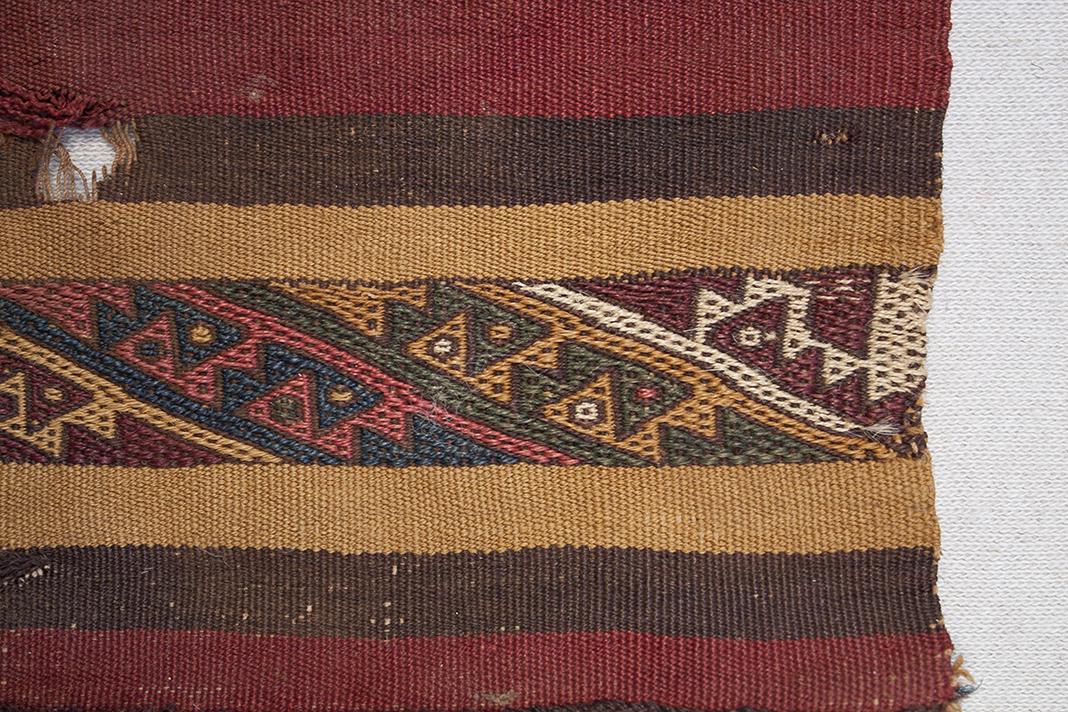
\includegraphics[width=14cm]{../images/BML044_avant.jpg}
	\end{center}
    \caption{Endroit d'un fragment d'une tapisserie avec trames supplémentaires qui imite l'organisation d'un tissage à dominante chaîne. \\ Référence dans la base données : BML044.}
    \label{fig:BML044_avant}
\end{figure}

Cette tapisserie de l'Intermédiaire Tardif (1000-1470) découverte à Chancay sur la côte centrale péruvienne illustre parfaitement ce transfert technique. La bande centrale, représentant des figures entrelacées, imite la technique de tissage à dominante chaîne avec un comptage 2/2. On retrouve les points alternés présents sur tout le tissage, les lignes noires qui soulignent les zones colorées et les formes triangulaires. Tout comme le fait Sophie Desrosiers, pour démontrer qu'il s'agit bien d'une imitation, nous pouvons relever le textile et les trajets des fils grâce aux grilles mises au point par Cason et Cahlander en 1976 pour des textiles ethnographiques à dominante chaîne\footcite[p.~49-51]{casonArtBolivianHighland1976}. Á part un petit défaut sur le triangle blanc le plus à droite du schéma (qui est peut-être lié à la conservation du textile et à la qualité de la photographie), nous pouvons relever que l'arrangement des fils sur la face de la tapisserie imite parfaitement une technique de tissage à dominante chaîne.

\begin{figure}[!ht]
       \begin{center}
        		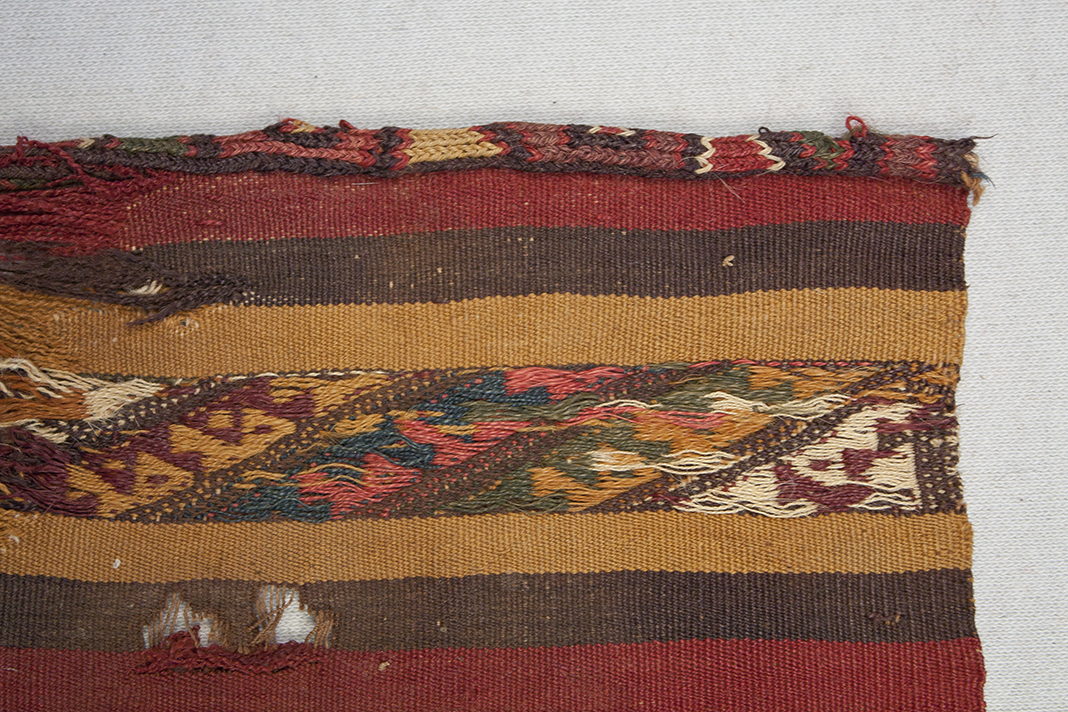
\includegraphics[width=14cm]{../images/BML044_arriere.jpg}
	\end{center}
    \caption{Envers d'un fragment d'une tapisserie avec trames supplémentaires qui imite l'organisation d'un tissage à dominante chaîne. \\ Référence dans la base données : BML044.}
    \label{fig:BML044_arriere}
\end{figure}

\begin{figure}[!ht]
       \begin{center}
        		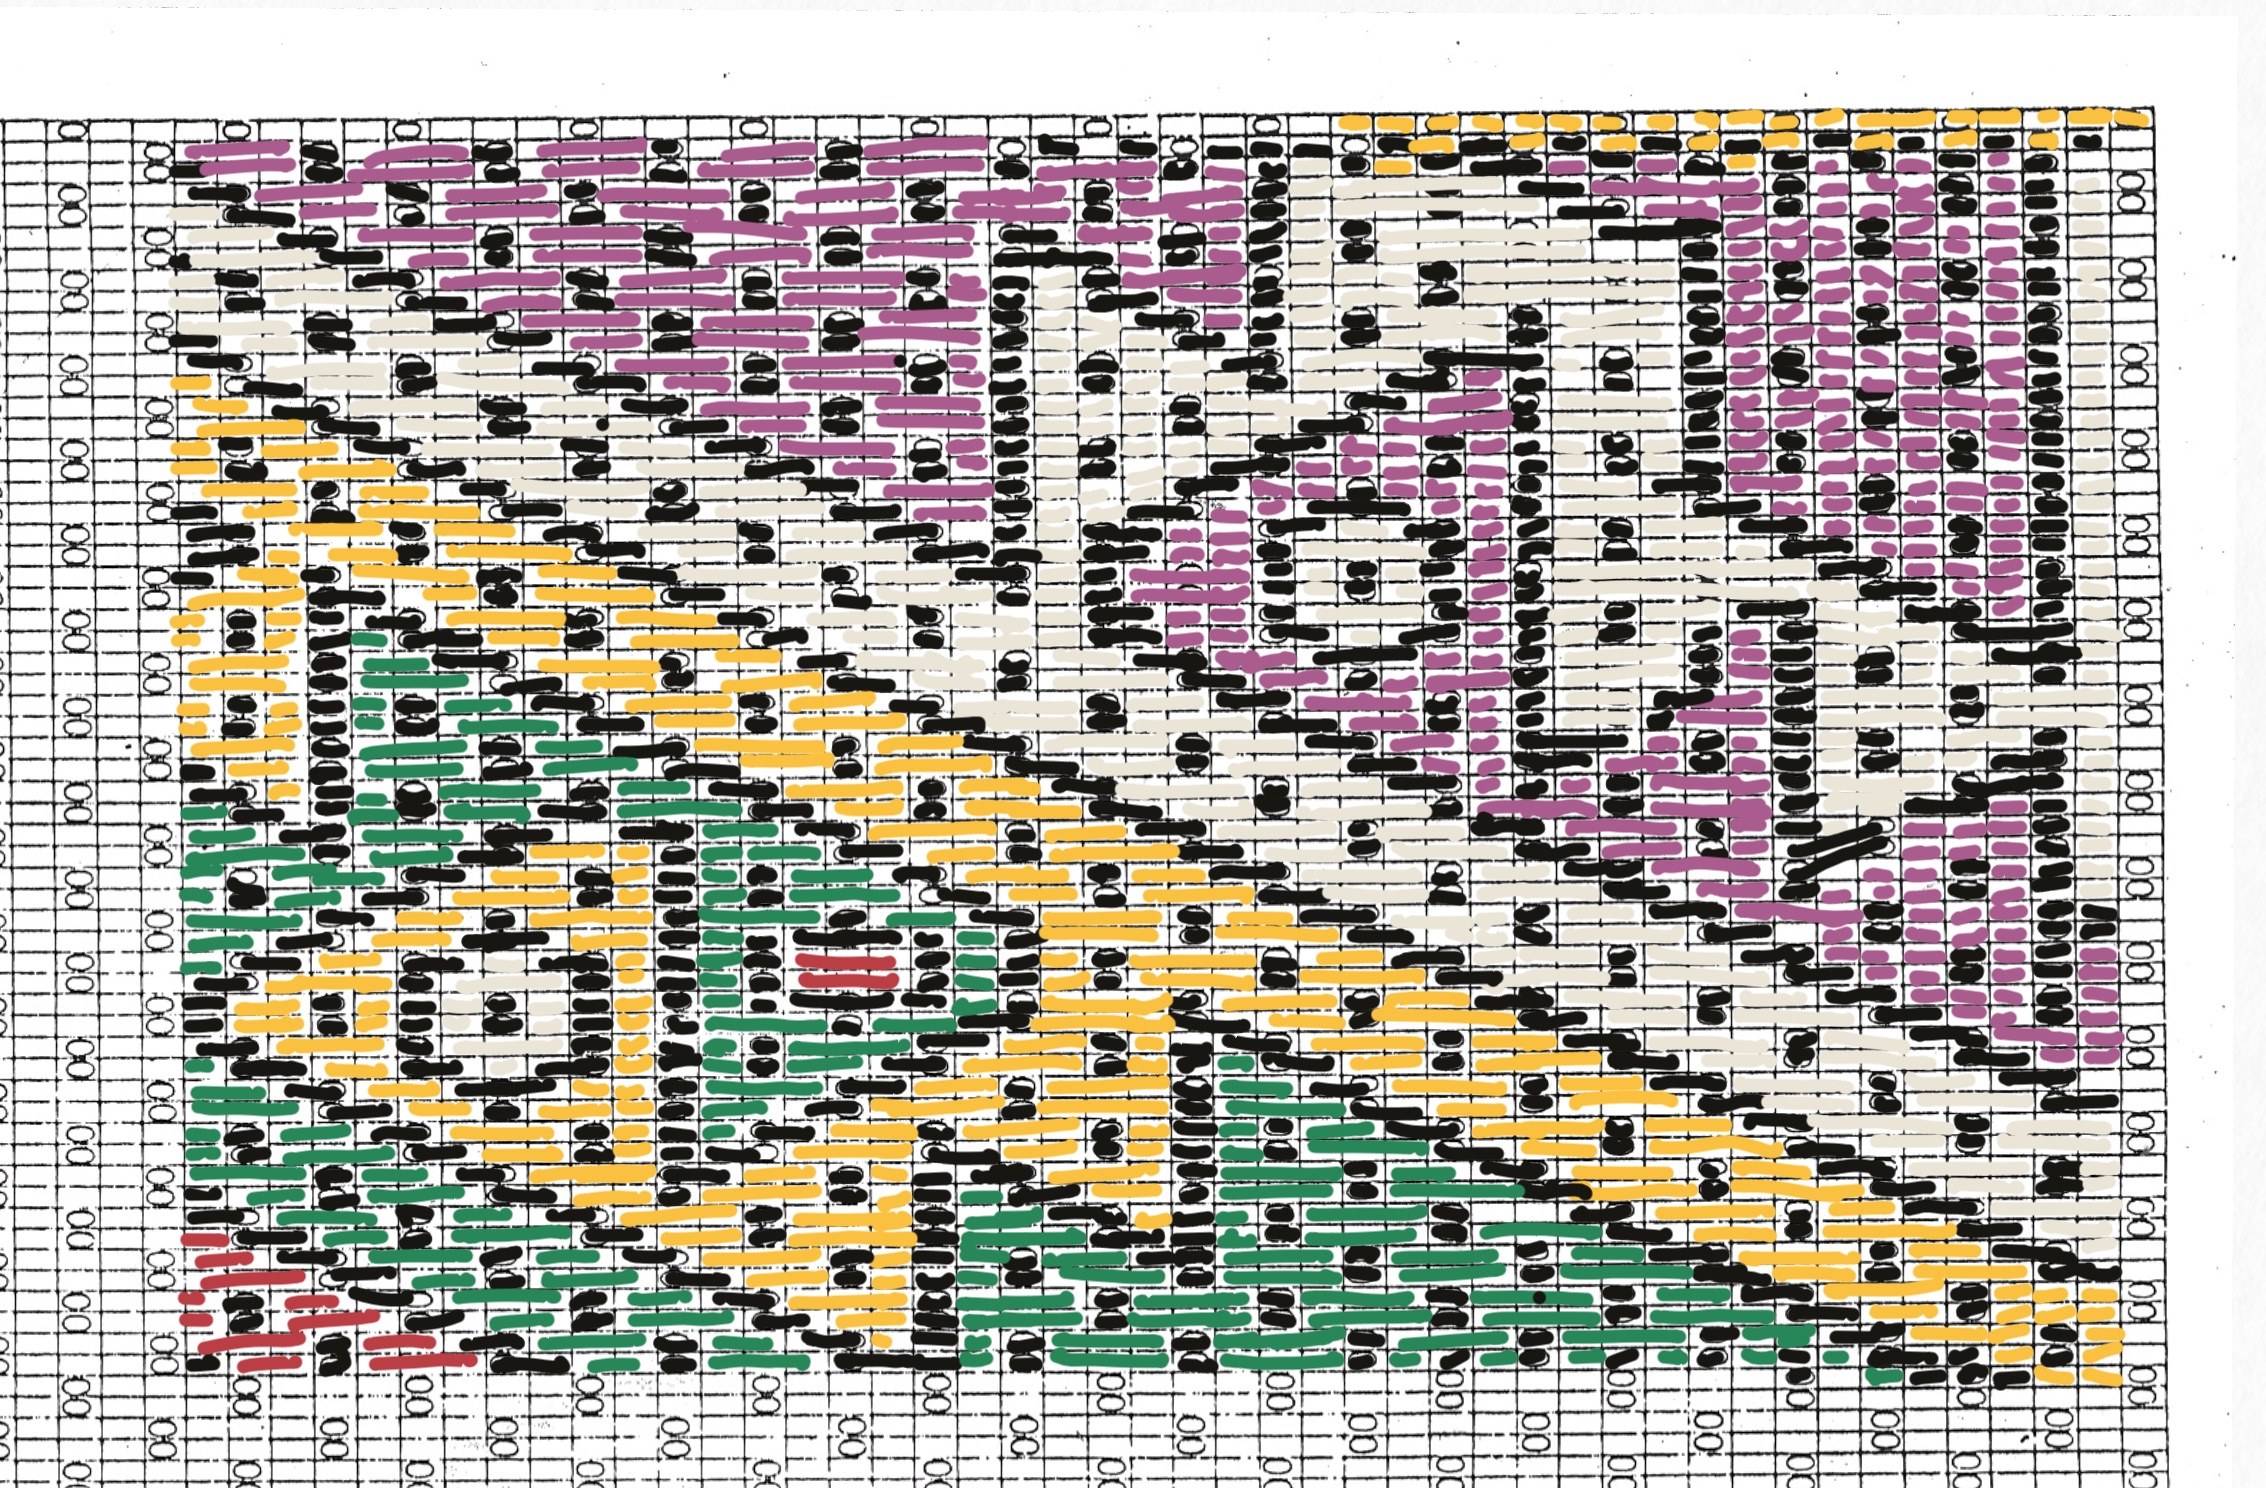
\includegraphics[width=14cm]{../images/BML044_schema.jpg}
	\end{center}
    \caption{Relevé partiel du textile BML044 sur une grille destinée à relever les tissage à dominante chaîne, tissés en comptage 2/2.}
    \label{fig:BML044_schema}
\end{figure}

Nous pouvons comparer cet exemple avec deux autres textiles de la base données réalisés en dominante chaîne avec un comptage 2/2. La similarité des traits caractéristiques de cette technique y est flagrante : délimitation des motifs en noir, points alternés sur toute la bande et formes triangulaires.

\begin{figure}[!h]
    \begin{minipage}[c]{.5\linewidth}
            \begin{center}
                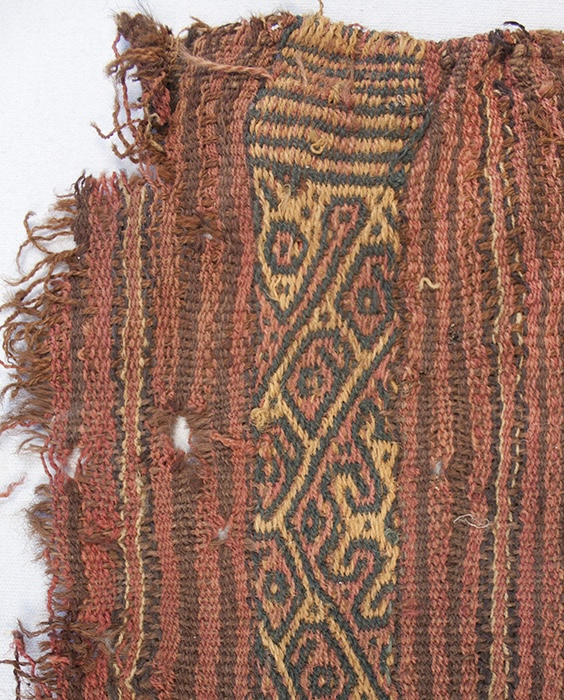
\includegraphics[height=7cm]{../images/BML019.jpg}
                 \caption{Tissage à dominante chaîne dont la bande centrale est composée avec 3 chaînes (comptage 2/2) de la période Intermédiaire Tardive, produit (?) et découvert sur la côte sud du Pérou. \\ Référence dans la base de données : BML019.}
            \end{center}
    \label{fig:BML019}
    \end{minipage}
    \hspace{5pt}
    \begin{minipage}[c]{.5\linewidth}
        \begin{center}
        		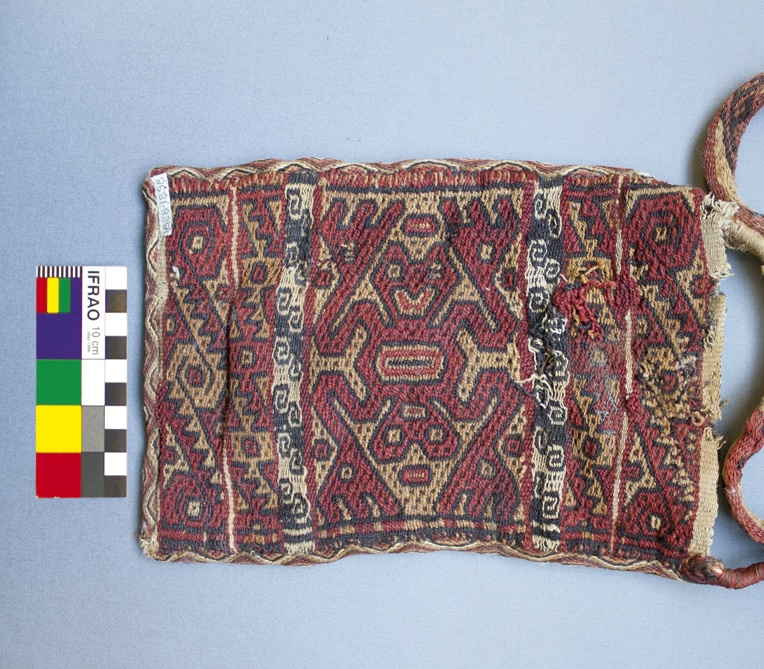
\includegraphics[height=7cm]{../images/VAM028.jpg}
		 \caption{Tissage à dominante chaîne dont la bande centrale a été composée avec 3 chaînes (comptage 2/2) de la période Intermédiaire Tardive, produit (?) et découvert sur la côte centrale du Pérou.  \\ Référence dans la base de données : VAM028.}
	\end{center}
    \label{fig:VAM028}   
    \end{minipage}
\end{figure}

Il est d'ailleurs intéressant de noter que la plupart des pièces présentant ce type d'imitations dans la base de données datent de l'Intermédiaire Récent, période au cours de laquelle les techniques de comptage des chaînes complémentaires sur la côte se sont multipliées : 
\begin{citer}
Leur multiplication pendant l'Intermédiaire Récent donne l'impression d'un langage commun qui a diffusé sur les côtes centrale et sud du Pérou pendant plusieurs siècles, véritables matrices géométriques venues des hautes-terres et fortement liées à des équilibres mathématiques induits par le tissage à dominante chaîne\footcite[p.~61]{desrosiersMatieresPremieresSavoirs2018}.
\end{citer}

\noindent Cette technique a également été imitée en broderie, comme le montre l'exemple suivant, plus ancien que les précédents, qui est composé d'une toile en coton sur laquelle sont brodés des motifs d'oiseaux et d'étoiles à huit branche en fibre de camélidés. Les points dans les pointes des étoiles et la délimitation en noir des motifs fait également penser à une imitation de la technique de tissage à dominante chaîne avec un comptage 2/2. L'imitation au sein des broderies a également été relevée par Sophie Desrosiers, cette fois-ci pour les pièces Paracas Necropolis (à la fin de l'Horizon Ancien et au début de l'Intermédiaire Ancien, soit entre -200 et 100)\footcite[p.~2]{desrosiersReexamenTuniqueOcucaje2010}. Dans ces deux cas d'imitation, en tapisserie ou en broderie, la complexité des textiles des hautes-terres par rapport à ceux produits sur la côte laisse à penser une antériorité du tissage avec chaînes complémentaires dans les hautes-terres\footcite[p.~8]{desrosiersHighlandComplementaryWarpWeaving2014}. 

Des réinterprétations liées à un contact entre les hautes-terres et la côte sont ainsi observables dans les textiles andins. Toutefois, ces phénomènes d'imitation restent difficiles à saisir puisque \og le groupe qui reçoit l'influence culturelle [...] adopte seulement certains aspects qui l'attirent plus ou qui ont plus de sens dans sa culture locale, et/ou adopte certaines caractéristiques culturelles avec des modifications\footnote{\cite[p.~10]{youngMontanaMarIntercambio2017}. Citation originale : \textquotedblleft \textit{el grupo que recibe la influencia cultural (es decir, el grupo que se apropia de otra cultura) solo adopte ciertos aspectos que le atraen más o que tienen más sentido dentro de su cultura local, y/o que adopte características culturales con modificaciones.}\textquotedblright}.\fg 

\begin{figure}[!ht]
       \begin{center}
        		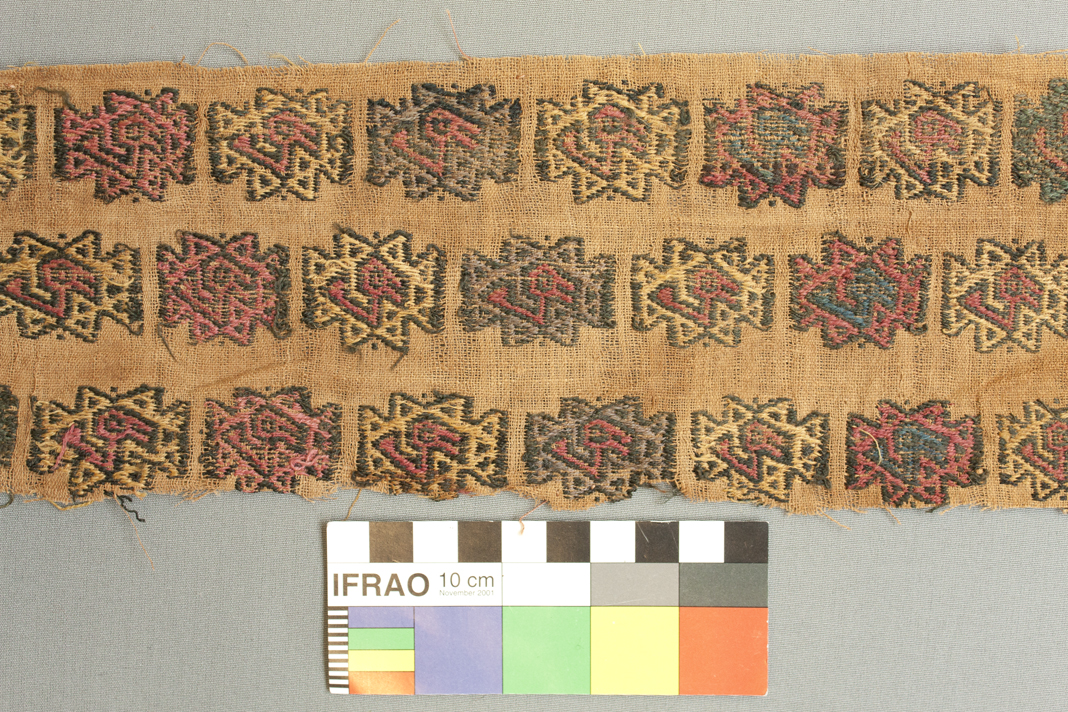
\includegraphics[width=11cm]{../images/VAM005.jpg}
	\end{center}
    \caption{Broderie de l'Intermédiaire Ancien, côte sud du Pérou.\\ Référence dans la base de données : VAM005.}
    \label{fig:VAM005}
\end{figure}

\subsection{La colonisation et les Indépendances : intenses périodes d'influences techniques et iconographiques}

\og À travers l'histoire, et plus particulièrement depuis le début de la période moderne, le textile peut être considéré comme le médium mondial par excellence\footcite[p.~21]{ferreiraTextilesPeriodeModerne2016}\fg. Dans les Andes, le début de la période moderne est en effet marqué par la Conquête espagnole qui favorise amplement la circulation du textile en tant qu'objet, comme nous l'avons montré dans la sous-partie précédente. Toutefois, ce flux n'est pas purement matériel. En plus des objets, des savoir-faire et des techniques circulent entre les continents.

Après la colonisation, les \textit{encomenderos}\footnote{Hommes ayant le statut de \textit{beneméritos} auprès de la Couronne espagnole qui leur confie le contrôle des sources de richesses et de la population tributaire sur un territoire déterminé. En échange, ils ont pour mission l'évangélisation de ces populations tout en les faisant travailler dans leurs exploitations.}, puis les riches familles créoles, installent dans toute la Vice-royauté des \textit{obrajes}, manufactures de textiles en laine de moutons\footcite{ortizdelatabladucasseObrajesObrajerosQuito1982}. En effet, des moutons sont importés par les colons espagnols et les \textit{encomenderos} détiennent de larges cheptels d'ovins. 
Les \textit{obrajes} sont organisés autour de métiers à tisser utilisés pour produire des lés de tissus à partir de la laine des moutons, destinés à la vente. Les \textit{obrajes} modifient radicalement l'outillage et imposent la spécialisation des tâches, suivant le processus de production hérité de l'Espagne médiévale. La laine est sélectionnée, lavée, cardée\footnote{Démêler la laine à l'aide de brosses appelées cardes.} et triée par les travailleurs de l'\textit{obrajes}. Puis elle est filée sur place ou par les femmes locales qui s'en occupent chez elles\footcite[p.49]{minogrijalvaManufacturaColonialConstitucion1993}. Ensuite, plusieurs ouvriers la tissent sur un large métier horizontal, invention médiévale européenne importée par les colons espagnols. Les étapes sont nombreuses et, à la suite du modèle médiéval, impliquent une division du travail avec un processus de production qui repose sur une \og spécialisation et [sur] le rythme continu et systématique de chaque fonction \fg\footnote{Ibid, p.~133.}. Un décalage apparaît alors entre la production textile antérieure à la colonisation qui reposait sur une auto-production, et l'organisation proto-industrielle coloniale destinée aux travailleurs des mines et à l'exportation. Les tissus produits sont grossiers et sont en partie destinés à la population indigène qui n'a plus le temps de produire pour sa propre consommation puisqu'elle travaille dans les mines et les \textit{obrajes}. Dans les faits, les \textit{obrajes} n'étaient pas des structures rentables par rapport à la production domestique. Ainsi, les coûts de production de la matière première et de construction des outils n'étaient compensés que par l'exploitation des travailleurs\footnote{Ibid, p.~132.}.
\begin{citer}
	Le transfert de la technologie textile européenne vers le monde américain n'impliqua apparemment pas un processus de résistance aux méthodes et aux outils jusqu'alors inconnus des travailleurs indigènes, mais, comme cela s'est produit dans d'autres secteurs du système colonial, il eut lieu autour de l'organisation et de l'intensité du travail\footnote{Ibid, p.~147. \textit{La transferencia tecnológica textil europea al mundo americano aparentemente no implicó un proceso de resistencia a métodos e instrumentos desconocidos hasta entonces por los trabajadores indígenas, sino, como sucedió en otros sectores del sistema colonial, se produjo en torno a la organización e intensidad del trabajo.}}.
\end{citer}
\noindent La colonisation marque donc une période de modification de l'organisation de la production textile, ainsi que l'introduction d'une nouvelle chaîne opératoire technique qui modifie radicalement les pratiques de production textile sur le territoire.

\begin{figure}[!ht]
       \begin{center}
        		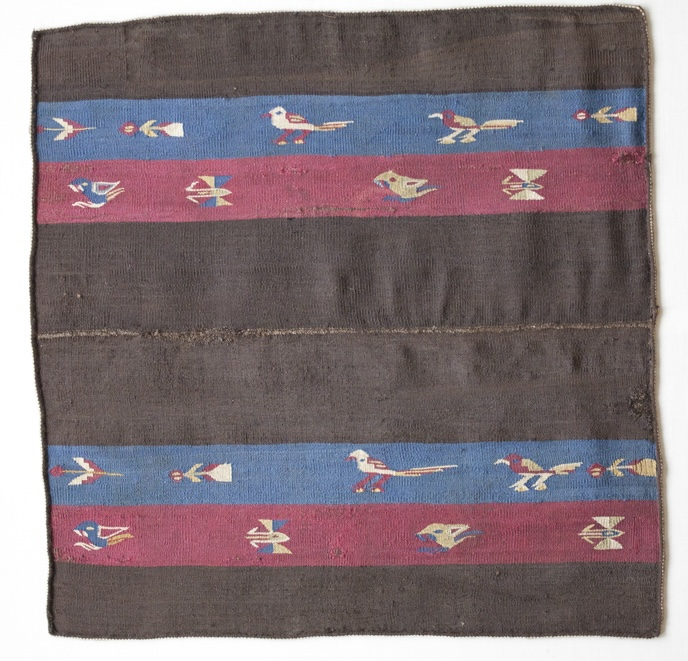
\includegraphics[width=12cm]{../images/MSF102.jpg}
		\caption[Tapisserie coloniale bolivienne avec motifs figuratifs]{Tapisserie coloniale bolivienne avec motifs figuratifs.	\protect\footnotemark \\ Référence dans la base de données : MSF102.}
	\label{fig:MSF102}
	\end{center}
\end{figure}
\footnotetext{La base de données en contient peu de textiles coloniaux, seulement 15 objets. Ceux-ci sont principalement en bandes unies de couleurs (ou \textit{pampa}) sans motifs, excepté cet exemple.}


Les Espagnols importent non seulement des techniques, au sein de la Vice-royauté du Pérou, mais aussi des savoirs puisque des guildes d'artisans européens se forment. Elena Phipps développe l'hypothèse selon laquelle les artisans européens ont formé des artisans locaux aux techniques médiévales européennes, hors du cadre des \textit{obrajes}, relevant que certains maîtres brodeurs portent des noms d'origine quechua\footcite[p.~37]{phippsIberianGlobe2013}. 
L'iconographie textile andine s'hybride rapidement à la fois entre artisans mais aussi par l'influence des colonisateurs sur la noblesse indigène, Monica Solorzano Gonzales présente ainsi différentes tapisseries au sein desquelles les motifs incas et espagnols sont mélangés\footcite[p.~499-500]{solorzanogonzalesTapizAndinoNobleza2020}. Ainsi, l'\textit{ahuayo} colonial précédent est en tapisserie de fils en poils de camélidés avec une couture centrale, éléments préhispaniques qui ont perduré après la colonisation. Toutefois, les motifs figuratifs héritent de la représentation médiévale européenne et non de la représentation préhispanique.
Cette intégration des motifs européens suit la demande des colons, non sans tension. Dans la région de Jauja des désaccords émergent ainsi entre les \textit{caciques}, gouverneurs locaux autochtones, et les \textit{encomenderos}, colons espagnols propriétaires terriens. Ces derniers requièrent aux artisans textiles des modifications stylistiques qui \og en plus de perturber le style propre de la région, signifiai[ent] plus de travail et de ressources\footnote{\cite[p.~124]{ramosTejidosSociedadColonial2010}. Citation originale : \textquotedblleft \textit{lo que además de perturbar el estilo propio de la región, significaba más trabajo y recursos}\textquotedblright}.\fg \:Ce conflit prend une telle importance que le roi Philippe II envoie une cédule royale en faveur des \textit{caciques}\footnote{Idem.}. Les conventions artistiques européennes intègrent toutefois le répertoire des tisserands andins, qui deviennent familiers avec la tradition textile européenne dès le \siecle{xviii}\footcite[p.~60]{nilesArtistEmpireInca1994}. \\

Les Indépendances, dans les années 1820, marquent la fin des \textit{obrajes} et la production textile cesse d'intéresser les historiens, alors même qu'elle perdure dans les communautés de manière \og traditionnelle\fg \:et qu'elle est faite de manière industrielle pour les vêtements de ville. Ainsi, à notre connaissance, aucun travail ne propose d'analyser les phénomènes d'imitation sur les textiles républicains et contemporains, d'autant plus que dans les années 1970, l'intérêt croissant des touristes et des collectionneurs pour le textile pousse les tisserands à vendre leurs pièces les plus anciennes\footcite[p.~242]{zornModernTraditionsImpact1990}. La marchandisation du textile modifie son statut dans la société et le fait davantage circuler. Ainsi, les motifs qui étaient traditionnellement propres à chaque communauté se diffusent aux autres communautés : 
\begin{citer}
 Dans le cas des tissages, par exemple, les \textit{pallais}\footnote{Le terme \textit{pallais} est un terme quechua qui désigne les motifs présents sur les tissages.} traditionnels disparaissent et d'autres, nouveaux, apparaissent ; de même, les \textit{pallais} qui étaient propres à une communauté ne le sont plus puisque, dans le processus de commercialisation, les communautés se copient les unes les autres, la finalité étant aujourd'hui de vendre le produit et non pas de distinguer chacune des communautés à travers tels aspects spécifiques des tenues\footnote{\cite[p.~9-10]{contrerashernandezProduccionArtesanalAndes1982} \textquotedblleft \textit{En el caso de los tejidos, por ejemplo, desaparecen} pallais \textit{tradicionales y aparecen otros nuevos; asimismo,} pallais \textit{que eran propios de una comunidad dejan de serlo ya que, debido al proceso de comercialización, unas comunidades los copian de otras pues la finalidad ahora es vender el producto y no diferenciarse unas comunidades de otras mediantes aspectos específicos del vestido.}\textquotedblright \:(sic.)}. (\textit{sic.})
\end{citer}

\noindent Les textiles, et donc les motifs, circulent, s'imitent et intègrent une iconographie plus moderne. Ainsi, il est aujourd'hui possible d'observer des textiles avec des armes à feu ou des hélicoptères. L'intégration de ces motifs modernes peut dans certains cas être envisagée comme une résistance face à l'intérêt des touristes pour les textiles aux iconographies plus traditionnelles\footcite[p.~247]{zornModernTraditionsImpact1990}.\\

Les transferts techniques et iconographiques et les réinterprétations textiles sont donc nombreux au fil du temps sur toute la zone andine. Certaines monographies s'intéressent à ces cas mais, à notre connaissance, il n'existe pas de travaux surplombants sur cette question. Un tel travail, rendu possible par le recours aux méthodes computationnelles, permettrait de conforter l'hypothèse de Sophie Desrosiers et de tenter de saisir les nuances de ces influences sur le temps long.
%Ici on a aussi le travail d'Eva Fischer sur les médecins Kallawaya (https://digitalcommons.unl.edu/cgi/viewcontent.cgi?article=1000&context=pctix)

\begin{figure}[!h]
    \begin{minipage}[c]{.5\linewidth}
            \begin{center}
                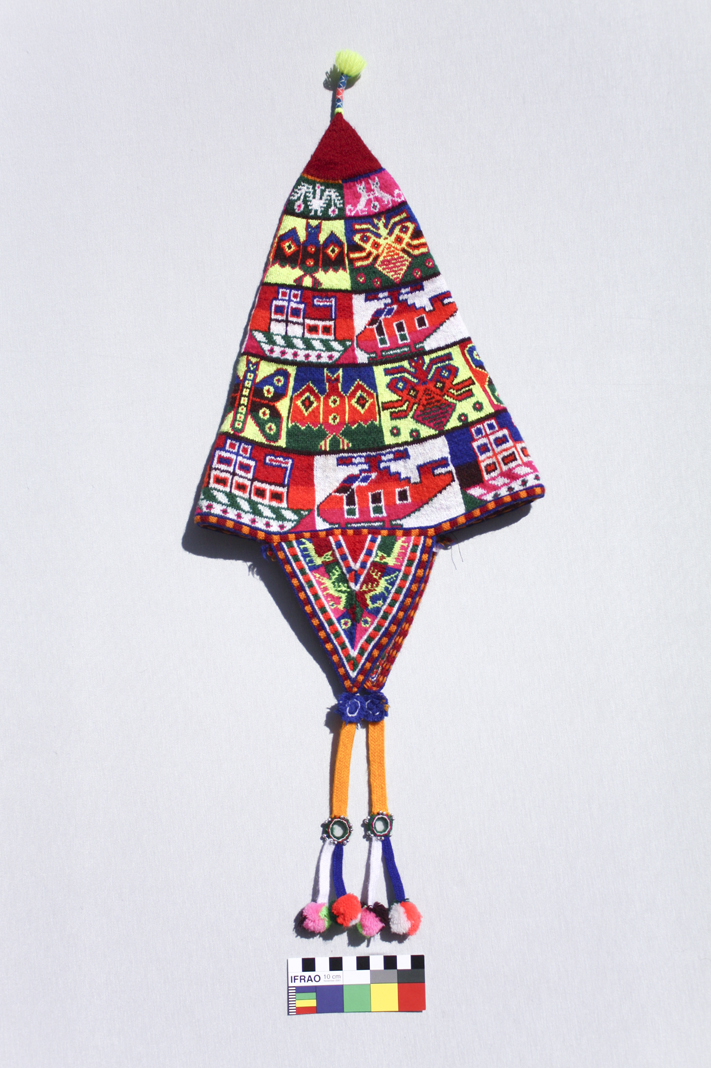
\includegraphics[height=10cm]{../images/ILCA049.jpg}
                 \caption{Bonnet contemporain tricoté en laine acrylique (Qaqachaka, Bolivie).\\ Référence dans la base de données : ILCA049.}
            \end{center}
    \label{fig:ILCA049}
    \end{minipage}
    \hspace{5pt}
    \begin{minipage}[c]{.5\linewidth}
        \begin{center}
        		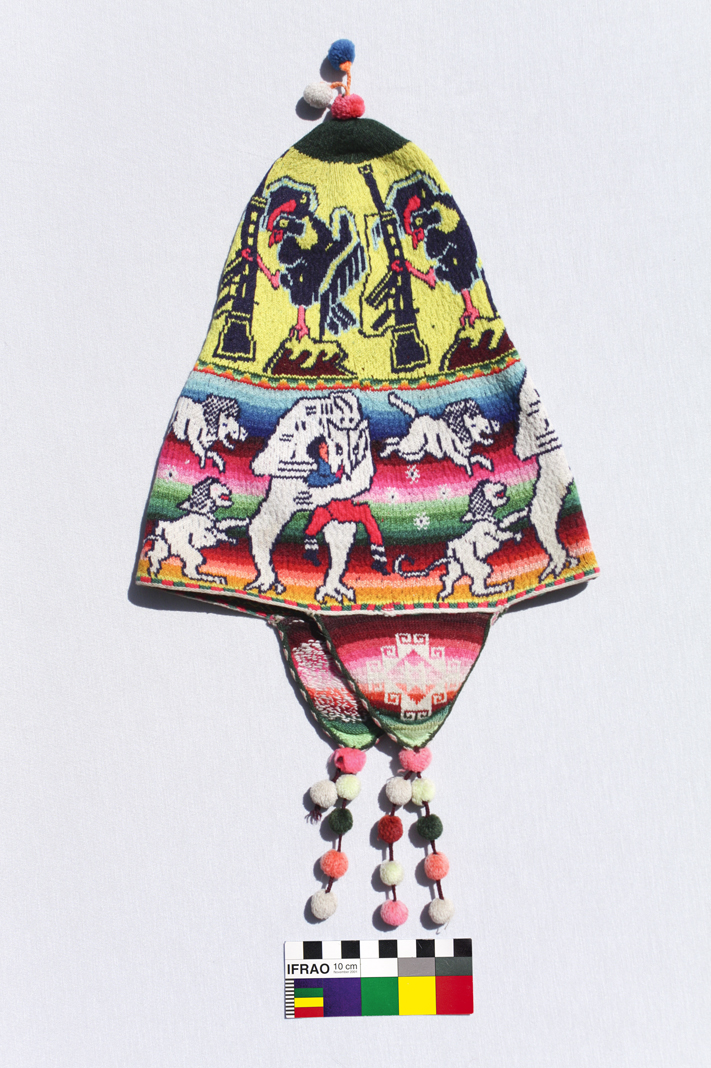
\includegraphics[height=10cm]{../images/ILCA045.jpg}
		 \caption{Bonnet contemporain tricoté en laine acrylique (Japo, Bolivie).\\ Référence dans la base de données : ILCA045.}
	\end{center}
    \label{fig:ILCA045}   
    \end{minipage}
\end{figure}


\section{La base de données \textit{Weaving Communities of Practice}}

Comme nous l'avons vu, saisir les circulations des textiles andins, ainsi que les influences de leurs techniques et de leurs iconographies est une tâche ardue qui nécessite d'avoir une vision globale sur un ample cadre-spatio temporel. C'est ce que propose la base de données que nous utilisons dans ce travail.

La base de données qui sert de fondement à notre analyse est rattachée au projet \textit{Weaving Communities of Practice. Textiles, Culture and Identity in the Andes. A Semiotic and Ontological Approach} (\og Tisser les communautés de pratiques. Textile, culture et identité dans les Andes. Une approche ontologique sémiotique \fg)\footnote{Lien vers le projet et la base de données : \url{http://weavingcommunities.org/}.}. Le projet a duré 3 ans, entre 2009 et 2012, et regroupait une équipe pluridisciplinaire, entre le CILAVS (Center for Iberian and Latin American Visual Studies), le Département d'informatique et des systèmes d'information à l'université de Birbeck (Londres, Royaume-Uni) et l'ILCA (Instituto de Lengua y Cultura Aymara, La Paz, Bolivie)\footcite{martinsExploringWeavingStructures2013}. Le regroupement des institutions a permis de rapprocher des collections bien souvent \og dispersées à travers le monde, ce qui rend difficile pour les chercheurs individuels d'avoir une perspective complète \fg\footnote{\cite[p.~3]{brownlowOntologicalApproachCreating2015}. Citation originale : \textquotedblleft \textit{scattered around the globe, making it hard for individual researchers to gain a full perspective}\textquotedblright}. Ce travail est d'autant plus important qu'il est bien souvent difficile de regrouper en un seul lieu les collections de musées différents. La démarche de la base de données souligne d'ailleurs ces problématiques d'interopérabilité entre les institutions puisque les données des musées ont été standardisées et complétées pour la majorité des artefacts. Une telle base de données est une source précieuse pour l'analyse des textiles, comme le souligne Brigitt Borkopp-Restle à propos du rôle des musées dans la présentation des textiles historiques : 
\begin{citer}
Les bases de données en ligne et, en particulier, les publications présentant des collections et des objets individuels avec des photographies de qualité et des informations détaillées sont donc d'autant plus précieuses : elles donnent accès à du matériel difficilement accessible autrement\footnote{\cite[p.~47]{borkopp-restleMuseumsMakingTextile2016}. Citation originale : \textquotedblleft \textit{Online databases and, in particular, publications that present collections and individual objects with good photographs and detailed information are therefore all the more valuable: they provide access to material not easily available otherwise.}\textquotedblright}.
\end{citer}

Comme son titre l'indique, ce projet d'analyse des textiles andins visait à mieux comprendre les pratiques de tissage des Andes au croisement des disciplines : anthropologie, histoire, archéologie et linguistique. L'approche pluridisciplinaire est centrale pour le textile. D'autant plus qu'une majorité des approches en histoire de l'art repose uniquement sur l'iconographie, laissant de côté les questions d'armure textile ou de contexte socio-historiques, pourtant nécessaires à la compréhension des pièces textiles dans les musées. Le projet a une visée universitaire mais est aussi destiné aux tisserand\inclusives{e} qui veulent faire reconnaître leur héritage et qui peuvent utiliser la base de données comme source d'information et d'inspiration pour leurs propres pratiques textiles. Il reposait sur trois axes historiques -- la culture Inca, la culture Tiwanaku et la culture Yampara (nord du Chili) -- mais, en réalité, elle référence près de soixante cultures différentes.

Le vocabulaire à l'intérieur de la base de données repose sur une ontologie en anglais, manipulée sous forme de tableurs, organisés en 30 documents contenant environ 1000 rangs chacun\footcite[p.~7]{brownlowOntologicalApproachCreating2015}. À notre connaissance, c'est la première tentative de modélisation ontologique dans le domaine du tissage andin. L'équipe a créé sa propre ontologie (OWL encodée en RDF c'est-à-dire reposant sur des triplets sujet-prédicat-objet) puisqu'elle considérait que l'ontologie CIDOC-CRM, proposant un vocabulaire muséal, n'était pas adapté à leurs objets. Les 696 pièces textiles sont donc expliquées par 39 catégories, elles-mêmes limitées par un vocabulaire déterminé.

\noindent Catégories utilisées dans la base de données : 
\begin{citer}
	\begin{itemize}
		\item \textbf{Identifiant du textile} : disponible pour toutes les pièces, il est composé de la manière suivante : ILCA\_\{institution source\}\_\{index de l'image\}. L'identifiant commence par ILCA pour \textit{Instituto de Lengua y Cultura Aymara} qui détient les images originales ainsi que leurs droits. La deuxième suite de lettres correspond à l'institution d'origine de la pièces textiles, et la suite de nombres à un index qui différencie les pièces textiles.
		\item  \textbf{Description du textile} : disponible pour toutes les pièces, il s'agit d'un texte libre en espagnol qui décrit le textile, il reprend les catégories suivantes sous forme de phrases.
		\item  \textbf{Photographies} : disponible pour toutes les pièces.
		\item  \textbf{Type de textile (usage)} : description de l'objet à travers son utilisation première : sac, vêtement, fragment, nappe etc. Le niveau de précision diffère grandement ainsi on a \og \textit{bag fragment} \fg, \og \textit{bag for hallucinogenic instruments} \fg\: et \og \textit{Fragment of bag for hallucinogenic instruments} \fg. À cela s'ajoute parfois des informations de couleurs \og \textit{golden mantle} \fg, de technique \og \textit{knitted cap} \fg \:ou de formes \og \textit{rectangular tunic} \fg.
Les termes sont principalement en anglais mais aussi en langues autochtones : \og \textit{pullo} \fg, \og \textit{Lliclla} \fg, \og \textit{incuña} \fg, \og \textit{huichi} \fg, \textit{ñañaka} \fg, \og \textit{pampa} \fg, \og \textit{iscayo} \fg...
		\item  \textbf{Période} : indique les périodes d'appartenance des pièces textiles.
		\item  \textbf{Musée d'origine} : disponible pour toutes les pièces, lieux où sont conservés les pièces textiles et source des informations. Le lieu de récupération est toujours website donc les informations ont uniquement été récupérée en ligne.
		\item \textbf{Lieu de production} : disponible pour toutes les pièces, lieu de production de la pièce textile.
		\item  \textbf{Lieu de découverte} : lieu où le textile a été découvert.
		\item  \textbf{Style (description selon la culture)} : style iconographiques des textiles, souvent rattaché à des cultures. Certaines catégories sont proches, par exemple, le style Tiwanaku se décline en \og \textit{Provincial Tiwanaku} \fg\: et \og \textit{Highland Tradition -- Tiwanaku} \fg.
		\item  \textbf{Motif} : descriptions des motifs figuratifs ou des formes géométriques. Ces descriptions sont aussi nombreuses qu'il y a de textiles.
		\item  \textbf{Attribut des motifs} : attribut associé au motif.
		\item  \textbf{Technique} : description des techniques utilisées pour faire le textile suivant la nomenclature proposée par D. Arnold et E. Espejo. Pour certaines pièces, la technique est accompagnée d'indications de couleurs.
		\item  \textbf{Structure} : disponible pour toutes les pièces, indication technique plus limitée (36 possibilités). Nomenclature qui se rapproche de celle proposée par I. Emery\footcite{emeryPrimaryStructuresFabrics1995}. 
		\item  \textbf{\og \textit{Fabric} \fg} : disponible pour toutes les pièces, indication technique encore plus limitée (11 possibilités). Il s'agit d'une description générale de l'armure des tissages dont la nomenclature se rapproche des grandes catégories proposées par I. Emery. 
		\item  \textbf{Culture} : cultures pré-hispaniques ou communautés contemporaines d'origine du textile (très proche de la catégorie style). Il s'agit à la fois de groupes linguistiques, de civilisations, de groupes ethniques et de lieux. Certaines cultures sont associées à des dates.
		\item  \textbf{Composition} : indication sur l'organisation du fond de la pièce (et non des motifs).		
		\item  \textbf{Composants} : description des différentes nappes de fils qui composent la pièce. Cette catégorie accepte trois termes (individuels ou combinées entre eux) : \og \textit{Extendend component} \fg, \og \textit{Structural component} \fg\: ou \og \textit{Added component} \fg.
		\item  \textbf{Matériel} : matériaux qui constituent la pièce textile.
		\item  \textbf{Numéro du fil} (de 1 à 6) et indication de son rôle de chaîne ou de trame pour les tissages. Pour chaque fil : 
			\begin{itemize}
			\item  \textbf{Torsion du fil} : pas renseignée.
			\item \textbf{Type de torsion} : pas renseigné.
			\item  \textbf{Couleur(s) des brins} : pas renseignée.
			\item  \textbf{Épaisseur} : pas renseignée.
			\item  \textbf{Direction de la torsion} : pas renseignée.
			\end{itemize}
		\item \textbf{Couleur(s) du tissu} : 21 couleurs qui peuvent être combinées pour décrire le textile.
		\item  \textbf{Nombre de couches de couleurs} : pas renseigné.
		\item  \textbf{Contraste} : constraste entre les couleurs.
		\item  \textbf{Finitions} : finition du tissage, inclut notamment les descriptions des lisières.
		\item  \textbf{Scène} : si le textile renvoie à une scène de la vie paysanne, religieuse ou festive.
		\item  \textbf{Séquence} : information supplémentaire sur l'agencement des fils.
		\item  \textbf{Symétrie} : utilisation de termes mathématiques pour décrire les symétries observables dans l'organisation des couleurs et des motifs.
		\item  \textbf{Taille} : pas renseignée.
		\item  \textbf{Usage} : pas renseigné.
		\item  \textbf{Direction de la chaîne} : pas renseignée.
	\end{itemize}
\end{citer}

Nous pouvons observer que les huit catégories qui n'ont pas été utilisées sont des catégories techniques très précises. En outre, l'aspect linguistique (quechua ou ayamara), défendu par Denise Arnold au moment de la création de la base de données dans l'analyse des textiles\footcite[p.~2]{brownlowOntologicalApproachCreating2015}, ne se retrouve pas en tant que tel dans l"ontologie. Les noms historiques et géographiques ont, pour certains, une origine autochtone mais ne sont pas porteurs de sens pour l'analyse des textiles.\\

Les données proviennent de 13 musées et institutions patrimoniales différents, situés en Bolivie, au Chili, au Pérou et au Royaume-Uni. Ce sont ces institutions qui ont fourni les images de la base de données, ainsi qu'une partie des métadonnées, complétées par les chercheurs. Nous reviendrons plus tard dans le mémoire sur la répartition des textiles entre les différents musées. Nous pouvons toutefois déjà relever une spécificité propre à l'ILCA, 158 pièces de leur collection sont des \og maquettes textiles didactiques, modèle pour les motifs utilisées lors de la planification textile\fg\footnote{Description de ces maquettes au sein de la base de données, traduite de l'espagnol au français.}. Ces maquettes se distinguent des autres textiles de la base de données, elles fournissent des exemples de motifs mais avec l'introduction de baguettes pour mettre en valeur le passage des fils, elles rendent ainsi des motifs élargis, comme étirés.

\begin{figure}[!h]
    \begin{minipage}[c]{.5\linewidth}
            \begin{center}
                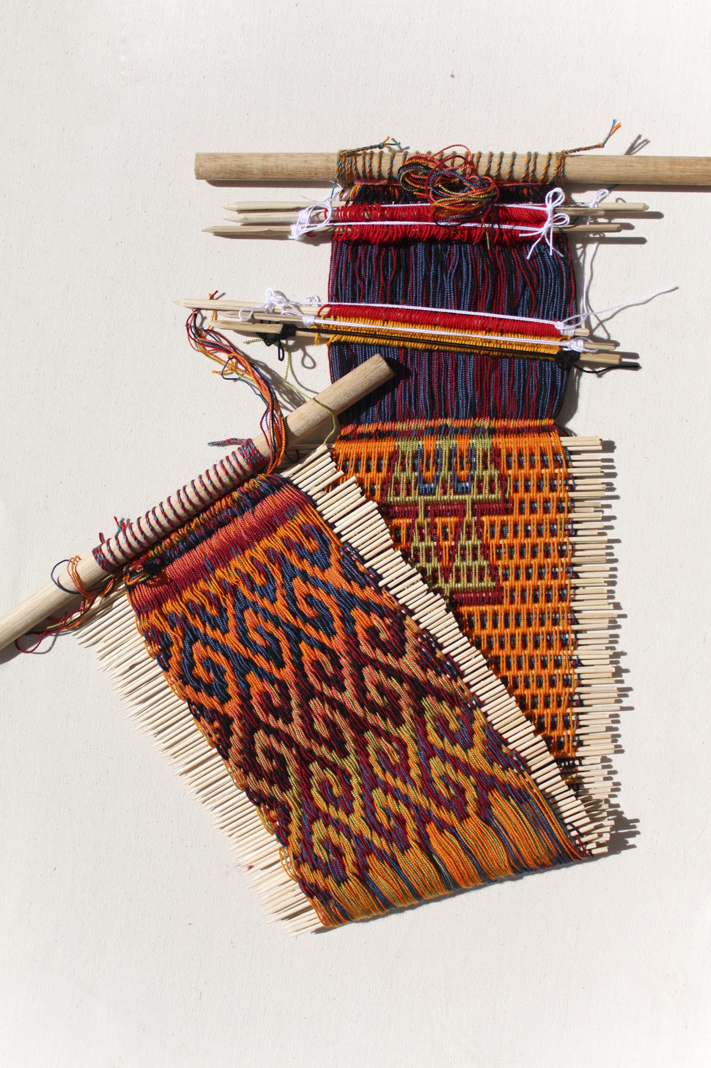
\includegraphics[height=8cm]{../images/MEE004B.jpg}
            \end{center}
    \label{fig:MEE004B}
    \end{minipage}
    \begin{minipage}[c]{.5\linewidth}
        \begin{center}
        		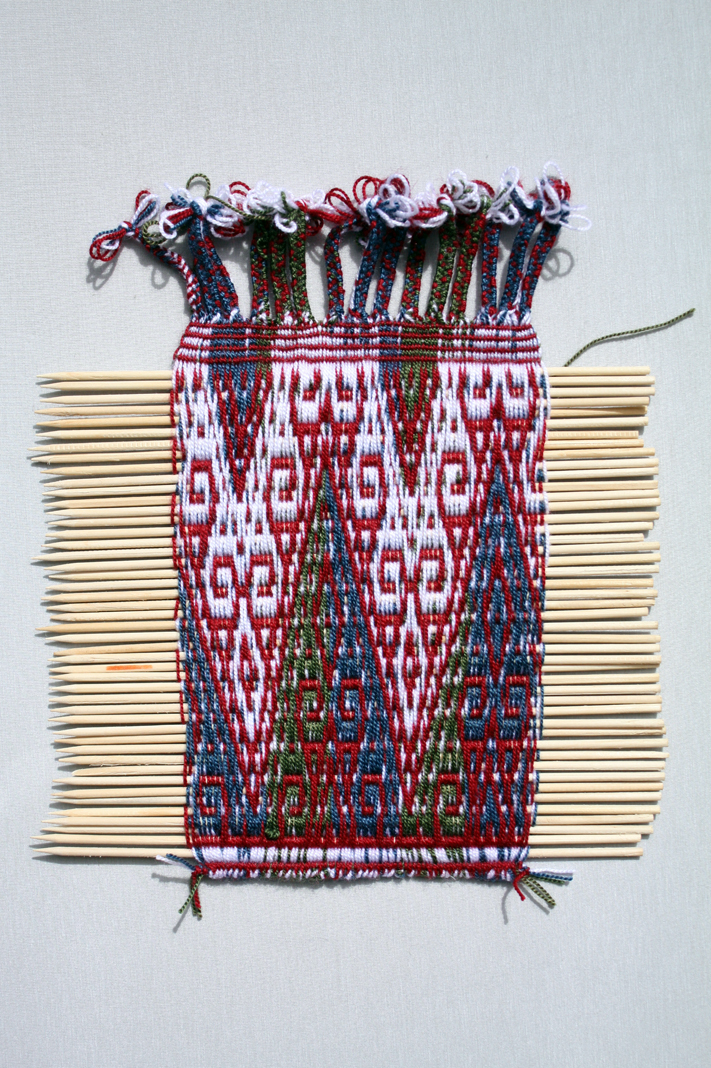
\includegraphics[height=8cm]{../images/MEE051.jpg}
	\end{center}
    \label{fig:MEE051}   
    \end{minipage}
     \caption{Maquettes réalisées par des tisserandes contemporaines.\\ Référence dans la base de données : MEE004B / MEE051.}
\end{figure}

Elles fournissent toutefois des éléments iconographiques importants des hautes-terres, et permettront une comparaison iconographique avec les autres textiles. Venant de différents musées, les photographies du corpus sont donc plutôt hétérogènes, facteur de complexité pour les analyses computationnelles. Nous verrons dans le chapitre suivant que cette hétérogénéité est également présente dans les métadonnées décrivant les textiles, nous proposerons différentes solutions pour pallier à ces déséquilibres dans le corpus.\\

\begin{figure}[!ht]
       \begin{center}
        		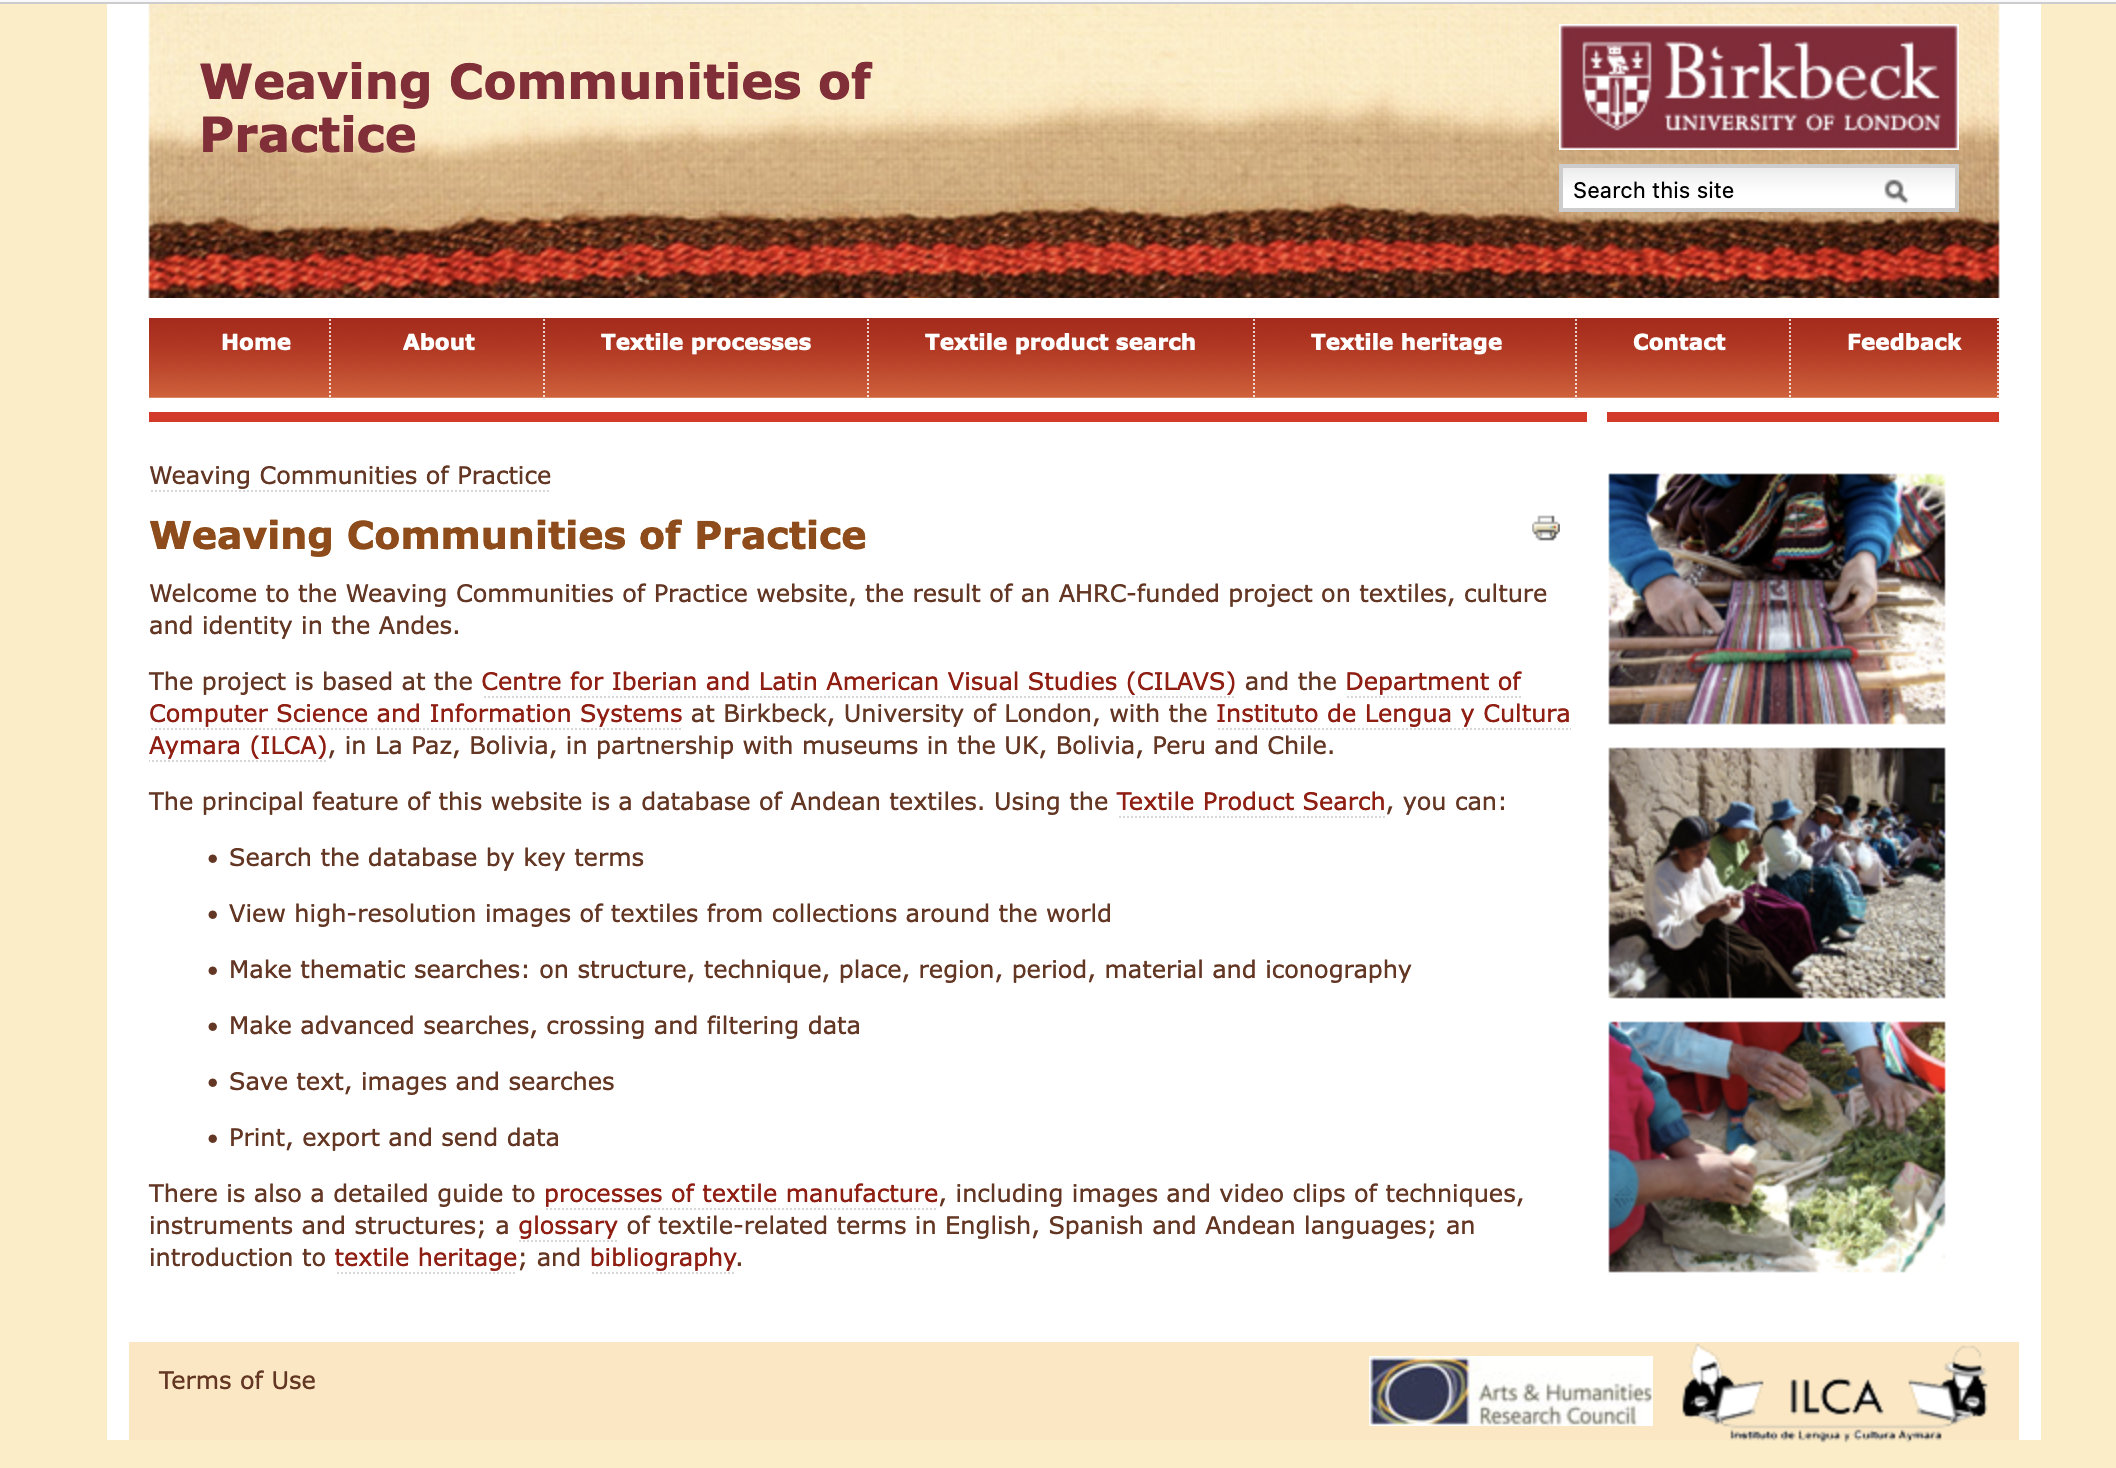
\includegraphics[width=12cm]{../images/screenWCP.png}
		\caption{Capture d'écran du site du projet \textit{Weaving Communities of Practice}.}
	\label{fig:WCP}
	\end{center}
\end{figure}

La réalisation d'un \textit{webscrapping} (récupération des données à partir d'un site Internet) a permis de récupérer les photographies et les métadonnées associées au textile dans un unique tableur, plus simple à manipuler.\\

\begin{figure}[!ht]
       \begin{center}
        		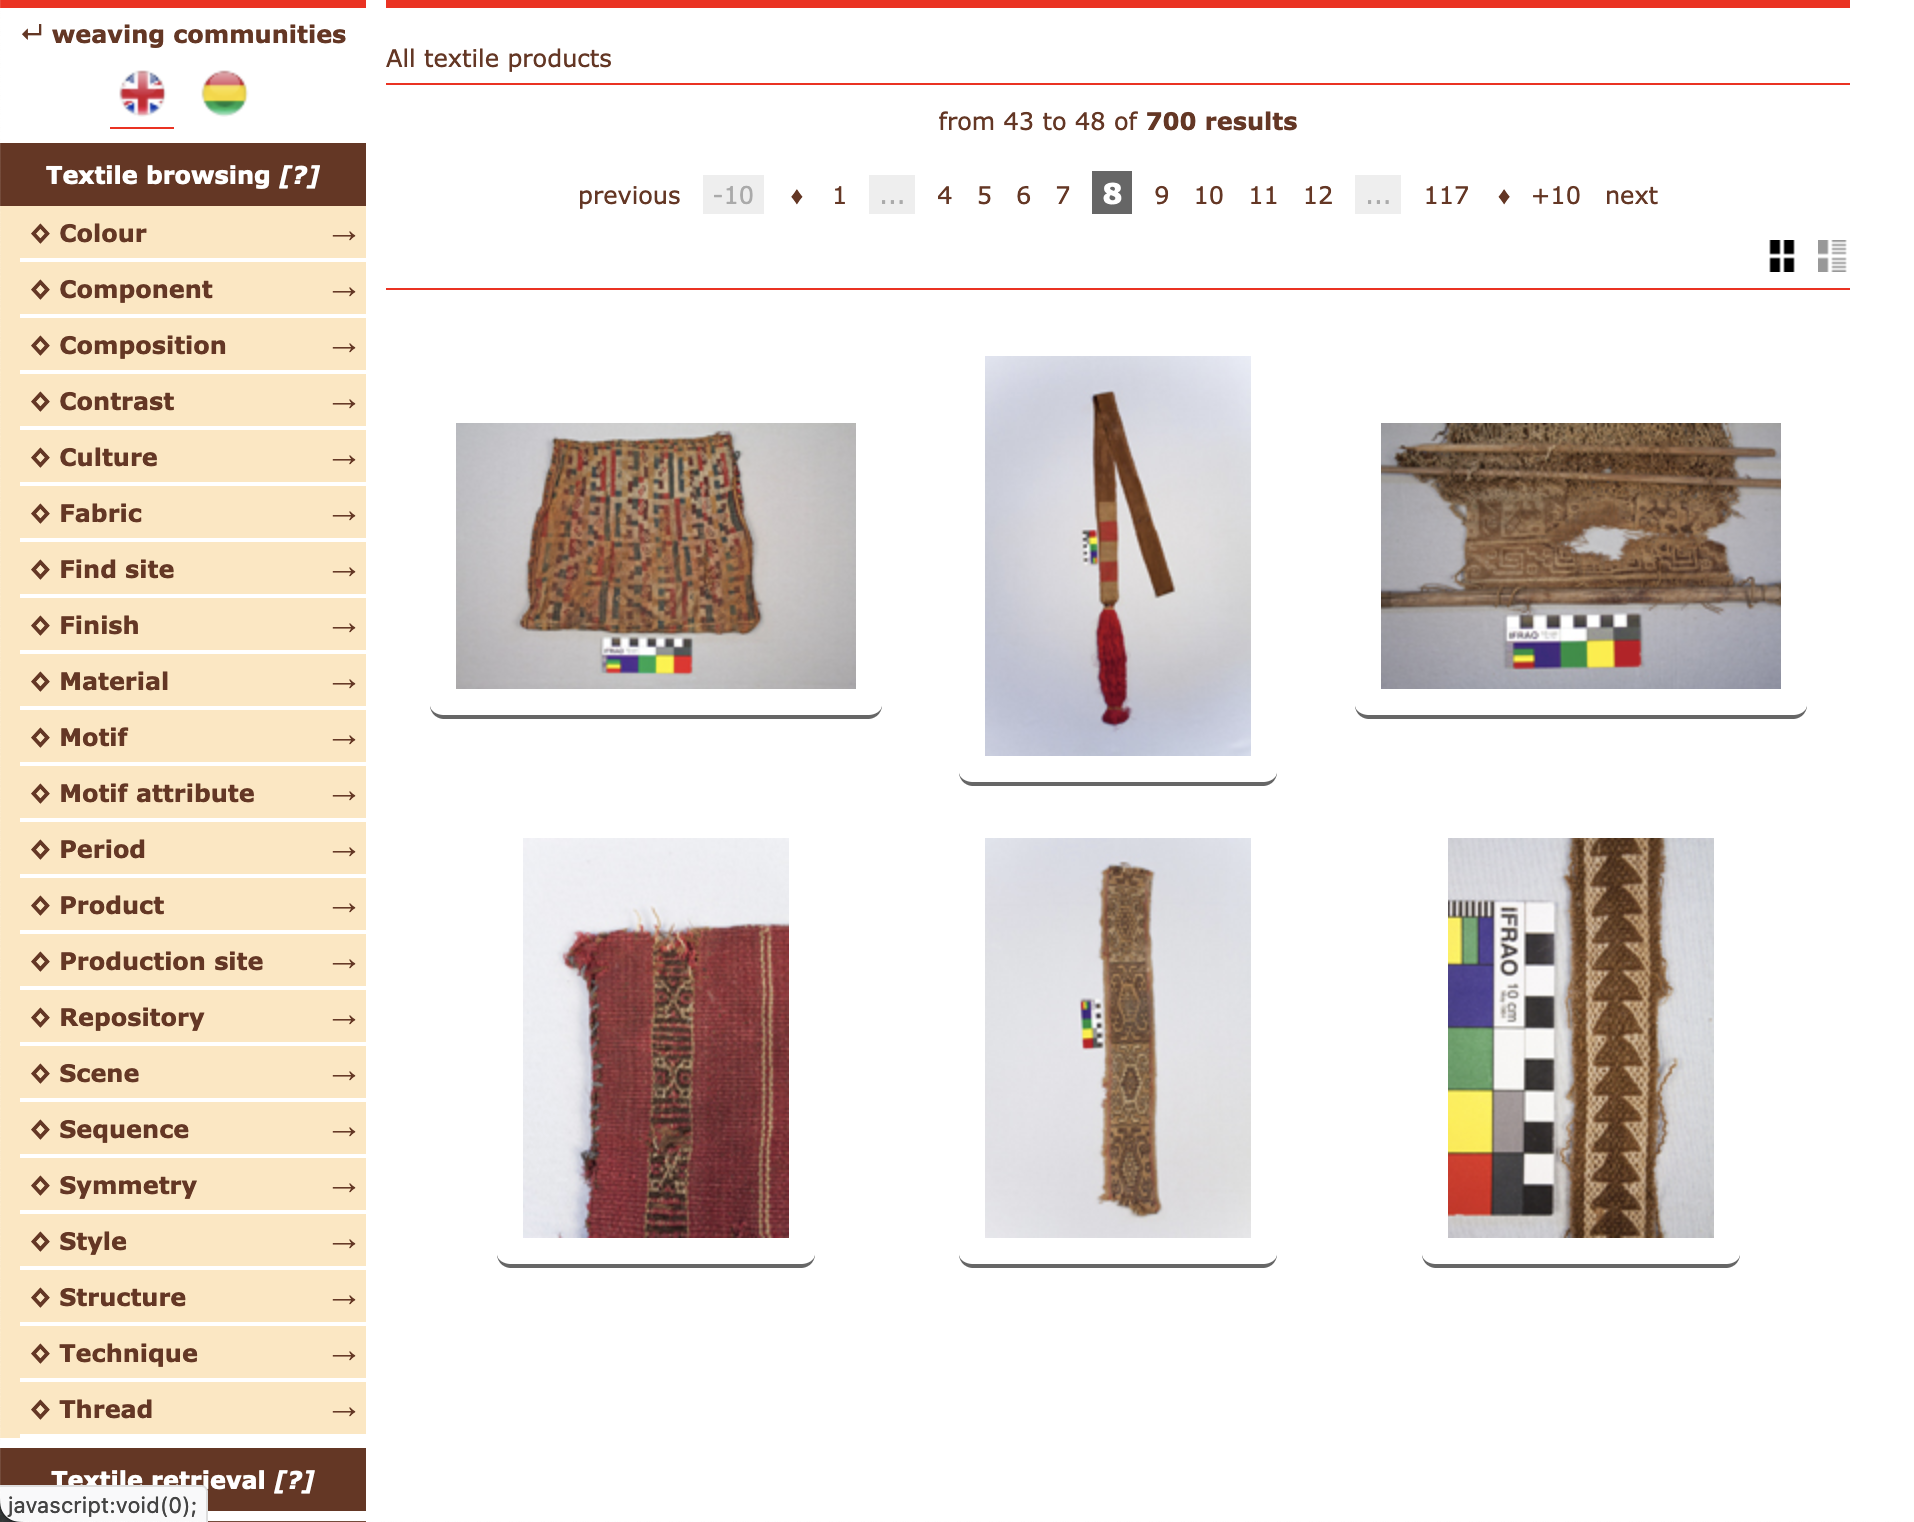
\includegraphics[width=12cm]{../images/screenWCPSearch.png}
		\caption{Capture d'écran de l'interface utilisateur de la base de données WCP.}
	\label{fig:WCPSearch}
	\end{center}
\end{figure}

Les données du projet \textit{Weaving Communities of Practice} semblent donc fournir un terrain fertile pour questionner l'état de l'art. Nous avons déjà pu observer quelques cas de mobilités et d'influences au sein de la base de données et le recours aux outils numériques va nous permettre d'élargir ces observations à l'ensemble des pièces textiles du corpus. 


\chapter{Une approche cartographique des textiles pour saisir leur répartition et leurs mobilités}
\markboth{}{}

\epigraph{\textquotedblleft Textiles move easily and designs and structures provoke imitations. Taking into consideration the style of the designs and the conditions of their creation will open new potential lines of fruitful research.\textquotedblright}{Sophie Desrosiers, 2014, \og Highland Complementary-Warp Weaving and the Lima Style in the Central Coast of Peru, ca. 200-650 C.E. \fg, p.~11.}


\section[Pré-traitement des données pour l'analyse géographique]{Pré-traitement des données pour l'analyse géographique}

\subsection{Homogénéiser les données}

À la suite de la récupération des données, une vue d'ensemble sur celles-ci nous permettra de mieux saisir leur organisation et leur constitution, ainsi que les pré-traitements nécessaires au travail d'analyse.

\subsubsection{Traitement des données manquantes}

La première étape de traitement des données consiste à inspecter la quantité de données manquantes pour chaque catégorie. 
Dans le cas de notre base de données, les données manquantes n'étaient pas toutes renseignées de la même manière. 
Certaines catégories étaient vides mais pour d'autres l'absence de données était indiquée par des chaînes de caractères (ensemble de lettres) et donc considérée comme une information au moment du traitement des données. 
J'ai détecté trois indications de ce type à partir de la reconstitution de l'ontologie de la base de données : \og \textit{unknown}\fg, \og \textit{unindentified fragment}\fg \:et \og \textit{NO DESCRIPTION AVAILABLE}\fg. Comme nous pouvons le voir, ces trois expressions n'indiquent pas l'absence de la même manière. La première indique une absence de connaissances (probablement lié au manque de contexte de certains textiles), la seconde indique l'impossibilité d'identifier l'utilité des textiles fragmentaires et la dernière correspond plutôt à une absence de données au sein de la base. Même si elles sont porteuses de sens, ces expressions sont remplacées par une valeur nulle (NaN) pour notre analyse, qui sera prise en compte comme telle au moment du traitement de données. Cette modification permet d'avoir une vision d'ensemble sur la base de données, de connaître le nombre d'informations disponibles pour chaque catégorie et donc de détecter celles qui sont les plus représentatives pour mener une analyse.

Cette modification permet d'obtenir le pourcentage réel de données manquantes de chaque catégorie comme nous pouvons le voir dans le tableau suivant : \\

\begin{table}[!h]
    \begin{tabular}{|p{0.3\textwidth}|p{0.3\textwidth}|p{0.3\textwidth}|}
        \hline
        \textbf{Nom de la catégorie} & \textbf{Pourcentage initial de données manquantes} & \textbf{Pourcentage final de données manquantes } \\ [3ex]\hline
         \textit{Style} & 22,55\% & 25,86\%\\[1ex] \hline
           \textit{Culture}& 25,43\% & 28,45\% \\ [1ex]\hline
           \textit{Product}& 0\% & 4,45\% \\ [1ex]\hline
    \end{tabular}
    \caption{Données manquantes avant et après modification.}
    \label{tab:NaN}
\end{table}  

Après ce traitement, nous pouvons observer la répartition des données disponibles par catégories dans la base de données. En moyenne, les catégories ont 47,73\% de valeurs manquantes. Toutefois, nous pouvons observer que seules 9 catégories sont complètement vides, et que 5 catégories sont au-dessus de 80\% de valeur nulle. À l'inverse, 6 catégories sont complètes et 14 catégories sont en-dessous de 10\% de valeur nulle, la médiane se situant à 36,93\%. Connaître les données manquantes nous permet de déterminer les catégories avec lesquelles il sera possible de travailler de manière représentative.

\begin{figure}[!h]
	\begin{center}
		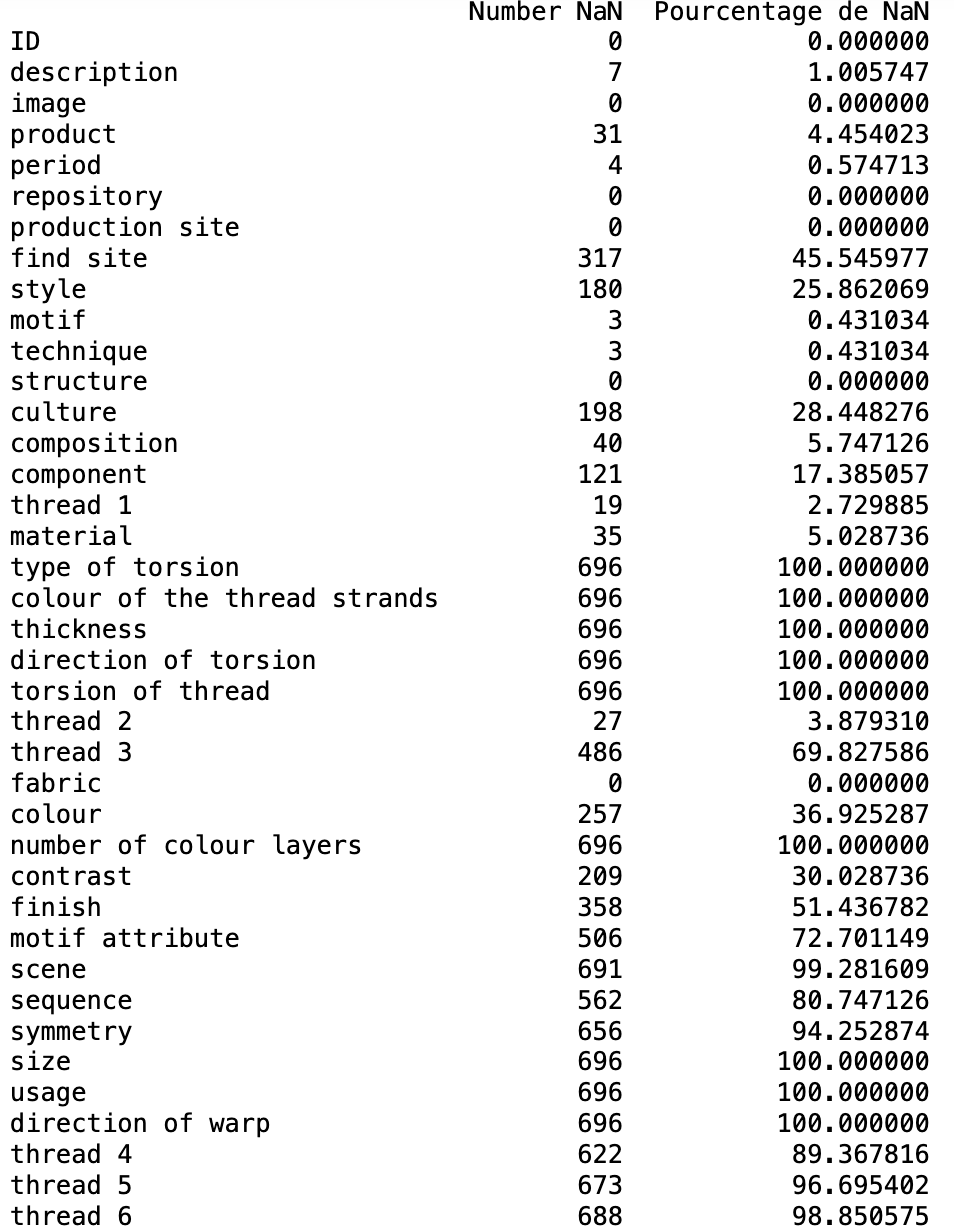
\includegraphics[width=9cm]{../images/NaN.png}
           	 \caption{Pourcentage de données manquantes par catégorie.}
           	 \label{NaN}
	 \end{center}
  \end{figure}


\clearpage


\subsubsection{Données historiques}

Un des intérêts du corpus étudié est sa profondeur historique qui permet une étude diachronique des pièces textiles. Les métadonnées associées aux pièces textiles nous fournissent la période de production de la pièce, ainsi qu'une datation approximative de cette même période pour 692 pièces (sur les 696 du corpus)\footnote{Voir le tableau récapitulatif des données indisponibles après traitement du tableur originel, image \ref{NaN}.}. Ces périodes reprennent la nomenclature archéologique traditionnellement utilisée pour les Andes, couvrant une temporalité allant de 1800 avant notre ère au temps présent.

\begin{figure}[!h]
	\begin{center}
		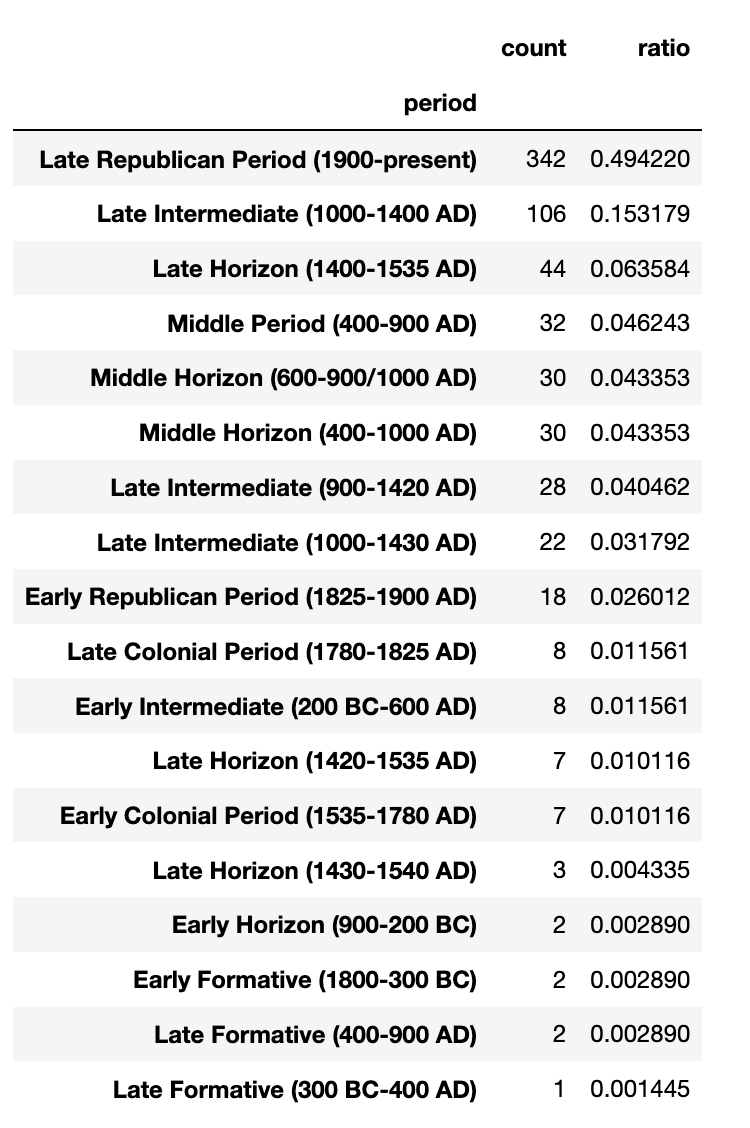
\includegraphics[width=10cm]{../images/periods_orig.png}
           	 \caption{Données chronologiques initiales}
           	 \label{chronoInit}
	 \end{center}
  \end{figure}
  
Malgré le recours à une ontologie lors de la création de la base de données, cette chronologie n'est pas uniformisée. Certaines périodes se superposent, d'autres couvrent la même période chronologique mais ne portent pas le même nom et certaines portent le même nom mais n'ont pas les mêmes dates de début et de fin, comme nous pouvons le voir sur le tableau \ref{chronoInit} et la frise chronologique \ref{chronoInitFri}. La variation des données biaise la compréhension statistique du corpus, c'est pourquoi il est nécessaire d'homogénéiser cette chronologie.
\clearpage

  \begin{figure}[!h]
	\begin{center}
		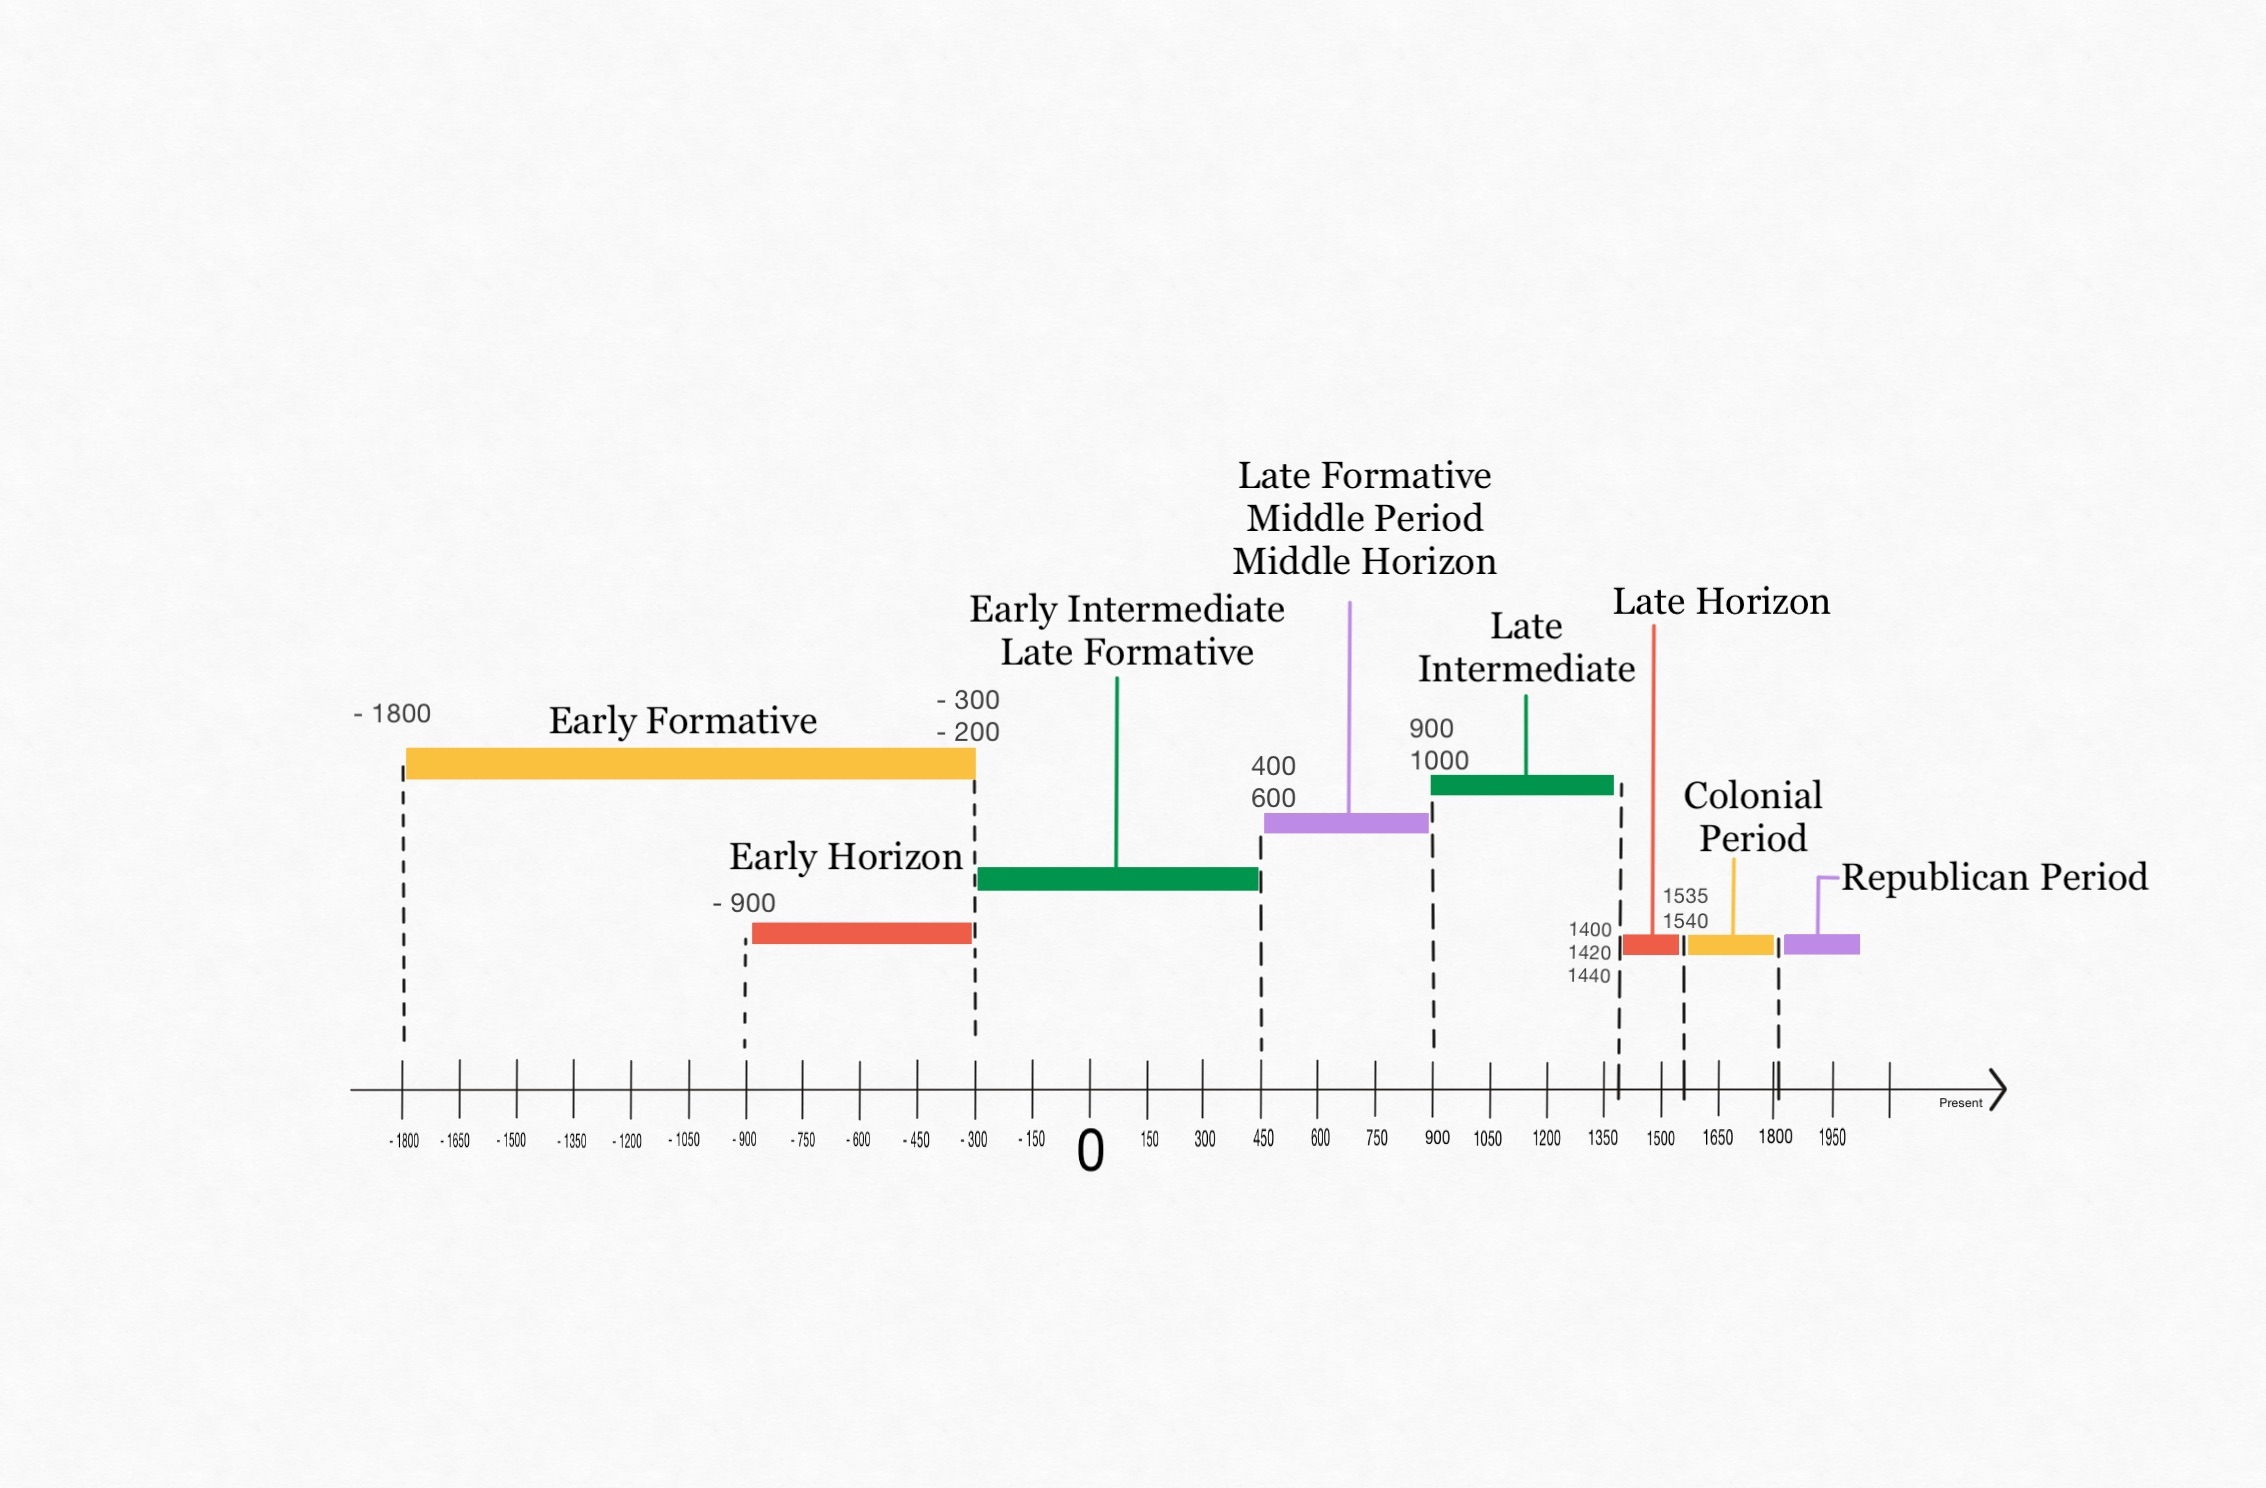
\includegraphics[width=15cm]{../images/FriseChronologiqueOrig.jpg}
           	 \caption{Frise chronologique représentant les données disponibles dans la base de données.}
           	 \label{chronoInitFri}
	 \end{center}
  \end{figure}


Ces difficultés de terminologie et de datation sont induites par le long débat académique qui a pris place entre différentes écoles d'archéologie andine. D'après l'historien et archéologue Gabriel Ramón Joffré, la périodisation en archéologie andine est nécessaire pour classifier les découvertes, mais elle est limitée par le manque de discussion dans la discipline autour des critères d'organisation chronologique\footnote{\cite[p.~7]{ramonjoffrePeriodificacionArqueologiaPeruana2005}}. Cela se traduit par une permanence des catégories définies au début de la discipline auxquelles s'ajoute une multitude de périodes hybrides accolant différents critères. Plus largement, la discipline se divise en deux courants de périodisation, d'une part les partisans de la périodisation évolutive et, d'autre part, ceux de la périodisation chronologique\footnote{Ibid., p.~8}. Ces deux courants ne s'opposent pas mais ont des fondements théoriques différents. En effet, la périodisation évolutive repose sur des critères économiques ou politiques, indiquant les évolutions des sociétés étudiées, alors que celle chronologique prend pour unique critère la temporalité relative des découvertes archéologiques. La compréhension des différents courants de périodisation nous permet de comprendre les choix chronologiques apparents dans la base de données et facilite l'homogénéisation des données. 

Les archéologues qui proposent les premières chronologies, à partir de la fin du \siecle{XIX} prennent pour références les zones géographiques où ils travaillent. Ainsi, Max Uhle et Alfred L. Kroeber proposent différentes chronologies à partir de leurs travaux sur la côte péruvienne (Pachacamac, vallées Moche...)\footnote{Ibid., p.~10}. Julio C. Tello, quant à lui, propose une chronologie à partir de la \textit{sierra}, les terres en altitude.
La deuxième génération d'archéologues péruviens et la troisième génération d'archéologues étrangers adoptent progressivement l'approche évolutionniste. Peu à peu \og la côte nord, et plus spécifiquement la séquence de la vallée de Virú, se convertit en modèle pour interpréter l'histoire de toute la zone andine\footnote{Ibid., p.~12]. Citation originale : \textquotedblleft \textit{la costa norte, y específicamente la secuencia del valle del Virú, se convirtió en el modelo para interpretar la historia de toda el área andina.}\textquotedblright}. \fg \:Toutefois, toujours selon Gabriel Ramón Joffré, l'approche évolutionniste pose problème puisqu'elle implique \og d'assumer la synchronie d'événements singuliers sur une large zone avec une -- supposée -- homogénéité séquentielle \footnote{\cite[p.~13]{ramonjoffrePeriodificacionArqueologiaPeruana2005}. Citation originale : \textquotedblleft \textit{se debe asumir sincronía de eventos semejantes en un área amplia con -- supuesta -- homogeneidad secuencial.}\textquotedblright}. \fg \: 

Dans les années 1960, l'archéologue étatsunien John Howland Rowe, qui avait souligné la difficulté d'obtenir une datation absolue des découvertes archéologiques\footnote{\cite{roweAbsoluteChronologyAndean1945}}, propose une périodisation relative, composée de 6 périodes\footnote{\cite[p.~627]{roweCulturalUnityDiversification1960}}. Il développe ces périodes à partir d'une chronologie relative entre la zone de référence et les zones étudiées, à partir de leurs similarités culturelles. Les pièces découvertes dans le même style sont considérées comme quasi-contemporaines. Les périodes sont donc des périodes larges car elles prennent en compte une temporalité de diffusion des styles : 

\begin{wraptable}{r}{0.6\textwidth}
    \centering
    \begin{tabular}{|c|c|}
        \hline
        \textbf{Classification J.H Rowe} & \textbf{Traductions françaises} \\[1ex] \hline
         \textit{Initial Period} & Période Initiale \\[1ex] \hline
          \textit{Early Horizon} & Horizon Ancien \\ [1ex]\hline
          \textit{Early Intermediate Period} & Période Intermédiaire Ancienne \\ [1ex]\hline
          \textit{Middle Horizon} &  Horizon Moyen \\[1ex] \hline
          \textit{Late Intermediate Period} &  Période Intermédiaire Récente\\[1ex] \hline
          \textit{Late Horizon} &  Horizon Récent \\[1ex] \hline
    \end{tabular}
    \caption{Tableau de la périodisation de J. H. Rowe (1960) et traductions françaises.}
    \label{tab:periodsTrad}
\end{wraptable} 
 
\begin{citer}
	Les périodes fondamentales du système péruvien sont assez longues, à l'exception de l'Horizon récent qui a duré environ 58 ans. Les périodes antérieures durent entre 300 et 700 ans\footnote{\cite[p.~50]{roweStagesPeriodsArchaeological1962}. Citation originale : \textquotedblleft \textit{The basic periods of the Peruvian system are quite long, except for the Late Horizon which lasted only 	about 58 years. The earlier periods range from 300 to 700 years in length. }\textquotedblright}.
\end{citer}

\noindent Le schéma chronologique de Rowe devient le cadre de référence de nombreuses prospections archéologiques dans les Andes\footnote{\cite[p.~19]{ramonjoffrePeriodificacionArqueologiaPeruana2005}}. Toutefois, une chronologie évolutionniste émerge comme modèle parallèle, proposée notamment par Luis Lumbreras, archéologue péruvien. Ce dernier est spécialiste des zones d'altitude qu'il prend comme références pour étendre sa chronologie aux découvertes archéologiques de la côte.

\begin{table}[!h]
   \centering
    \begin{tabular}{|p{0.3\textwidth}|p{0.3\textwidth}|p{0.3\textwidth}|}
         \cline{1-3}
         \multicolumn{2}{|c|}{ \textbf{Classification L. Lumbreras (et traduction)}} & \textbf{Classification J. H. Rowe} \\ [1ex]  \cline{1-3}
         \textit{Lítico} &  Litique & Pré-céramique \\ [1ex]\hline
          \textit{Arcaico (temprano, medio, tardío)} & Archaïque (ancien, moyen, tardif) & Pré-céramique \\ \hline
          \textit{Formativo (inferior, medio, superior)} & Formatif (inférieur, moyen, supérieur) & Période Initiale / Horizon Ancien \\ \hline
          \textit{Desarollos Regionales} & Développements régionaux &  Période Intermédiaire Ancienne\\[1ex] \hline
          \textit{Expansión Wari} & Expansion Wari &  Horizon Moyen \\[1ex] \hline
          \textit{Estados Regionales} & Stades régionaux & Période Intermédiaire Récente \\ [1ex]\hline
          \textit{Imperio del Tawantinsuyo} & Empire du \textit{Tawantinsuyu} & Horizon Récent \\ [1ex]\hline
    \end{tabular} 
    \caption{\centering Tableau de la périodisation de L. Lumbreras (1965), traductions françaises et équivalents simplifiés chez Rowe (1960).}
    \label{tab:periods}
\end{table}  

\clearpage

À la suite de ces propositions classificatoires, les différents archéologues continuent de mélanger les deux modèles, évolutionniste et chronologique. Par exemple, le terme de Formatif est parfois utilisé pour décrire la période Initiale, l'Horizon Ancien et la période Intermédiaire Ancienne (de 1500 avant notre ère à 200 après notre ère), libéré de toutes connotations évolutives\footnote{\cite[p.~22]{ramonjoffrePeriodificacionArqueologiaPeruana2005}}. 

Après le développement de la datation carbone qui permet une précision temporelle, bien que relative, des bornes chronologiques sont associées à chaque période de Rowe. Les variations de bornes chronologiques dans la base de données sont liées au point de référence de la chronologie. Ainsi, la période \og \textit{Late Formative}\fg, de 400 à 900 avant notre ère, correspond à la datation de cette période dans les vallées occidentales du sud du Pérou, alors que la datation de 300 avant notre ère à 400 après notre ère correspond à la datation de l'Altiplano bolivien\footnote{Romuald Housse, communication personnelle.}. Il en est de même pour le début de l'Horizon Récent qui correspond à la période d'extension de l'empire Inca : 1430 correspond au début de l'extension de la civilisation Inca autour de son foyer d'origine, Cuzco, alors que la date de 1470 correspond à la date de la chute de Chan Chan, capitale de l'empire côtier Chimú. 

\begin{table}[!h]
    \centering
    \begin{tabular}{|c|c|}
         \hline
        \textbf{Classification J.H Rowe} & \textbf{Consensus actuel de datation} \\[1ex] \hline         
        Période Initiale & 1800 - 900 avant notre ère  \\[1ex] \hline
         Horizon Ancien & 900 - 200 avant notre ère\\ [1ex]\hline
         Période Intermédiaire Ancienne & 200 avant notre ère - 600 \\[1ex] \hline
         Horizon Moyen & 600 - 1000 \\[1ex] \hline
          Période Intermédiaire Récente & 1000 - 1470 \\[1ex] \hline
         Horizon Récent & 1470 - 1535\\[1ex] \hline
    \end{tabular}
    \caption{\centering Tableau de la périodisation de J. H. Rowe (1960) et datation contemporaine à partir de A. Boissière, B, Faugère et N. Goepfert (éds., 2022).}
    \label{tab:periodsRowe}
\end{table}  

\begin{figure}[!h]
	\begin{center}
		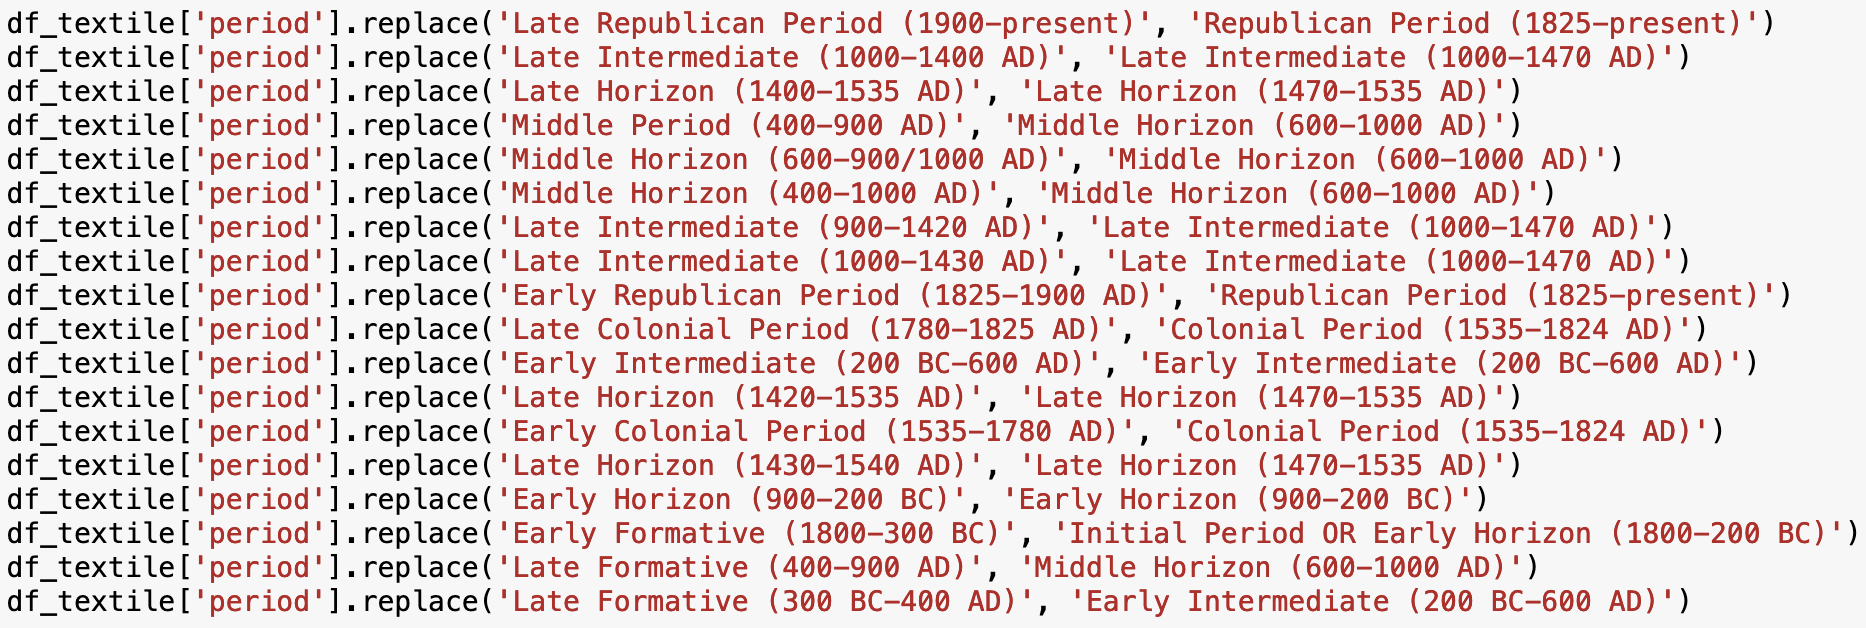
\includegraphics[width=15cm]{../images/periods_modif.png}
           	 \caption{Code utilisé pour modifier les données}
           	 \label{codeChrono}
	 \end{center}
  \end{figure}

La prise en compte de l'historiographie de la chronologie andine permet d'homogénéiser la chronologie de la base de données pour faciliter le traitement des données, sans pour autant perdre les informations chronologiques.
Nous passons alors de 18 périodes à 8 périodes. Cette réduction du nombre de plages chronologiques permet aussi une meilleure vue d'ensemble sur la répartition des données.

\clearpage

\begin{figure}[!h]
	\begin{center}
		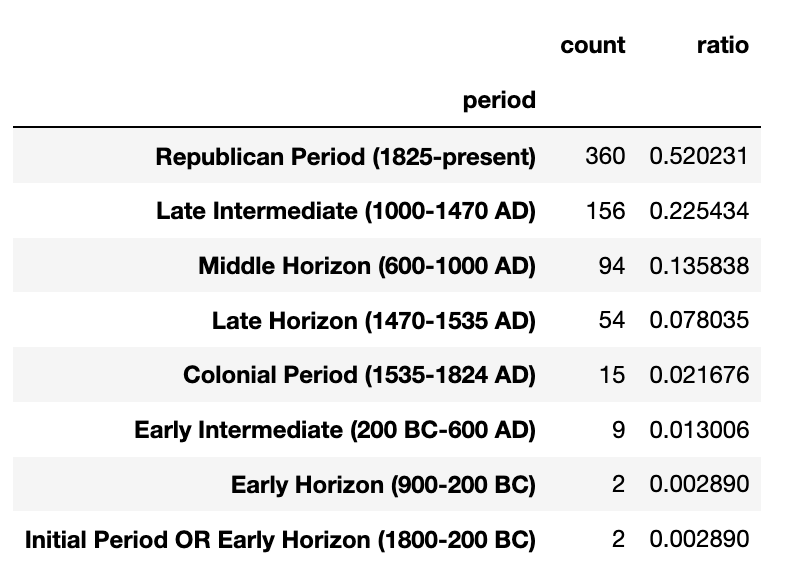
\includegraphics[width=10cm]{../images/periods_fin.png}
           	 \caption{Données chronologiques modifiées}
           	 \label{chronoFin}
	 \end{center}
  \end{figure}


  \begin{figure}[!h]
	\begin{center}
		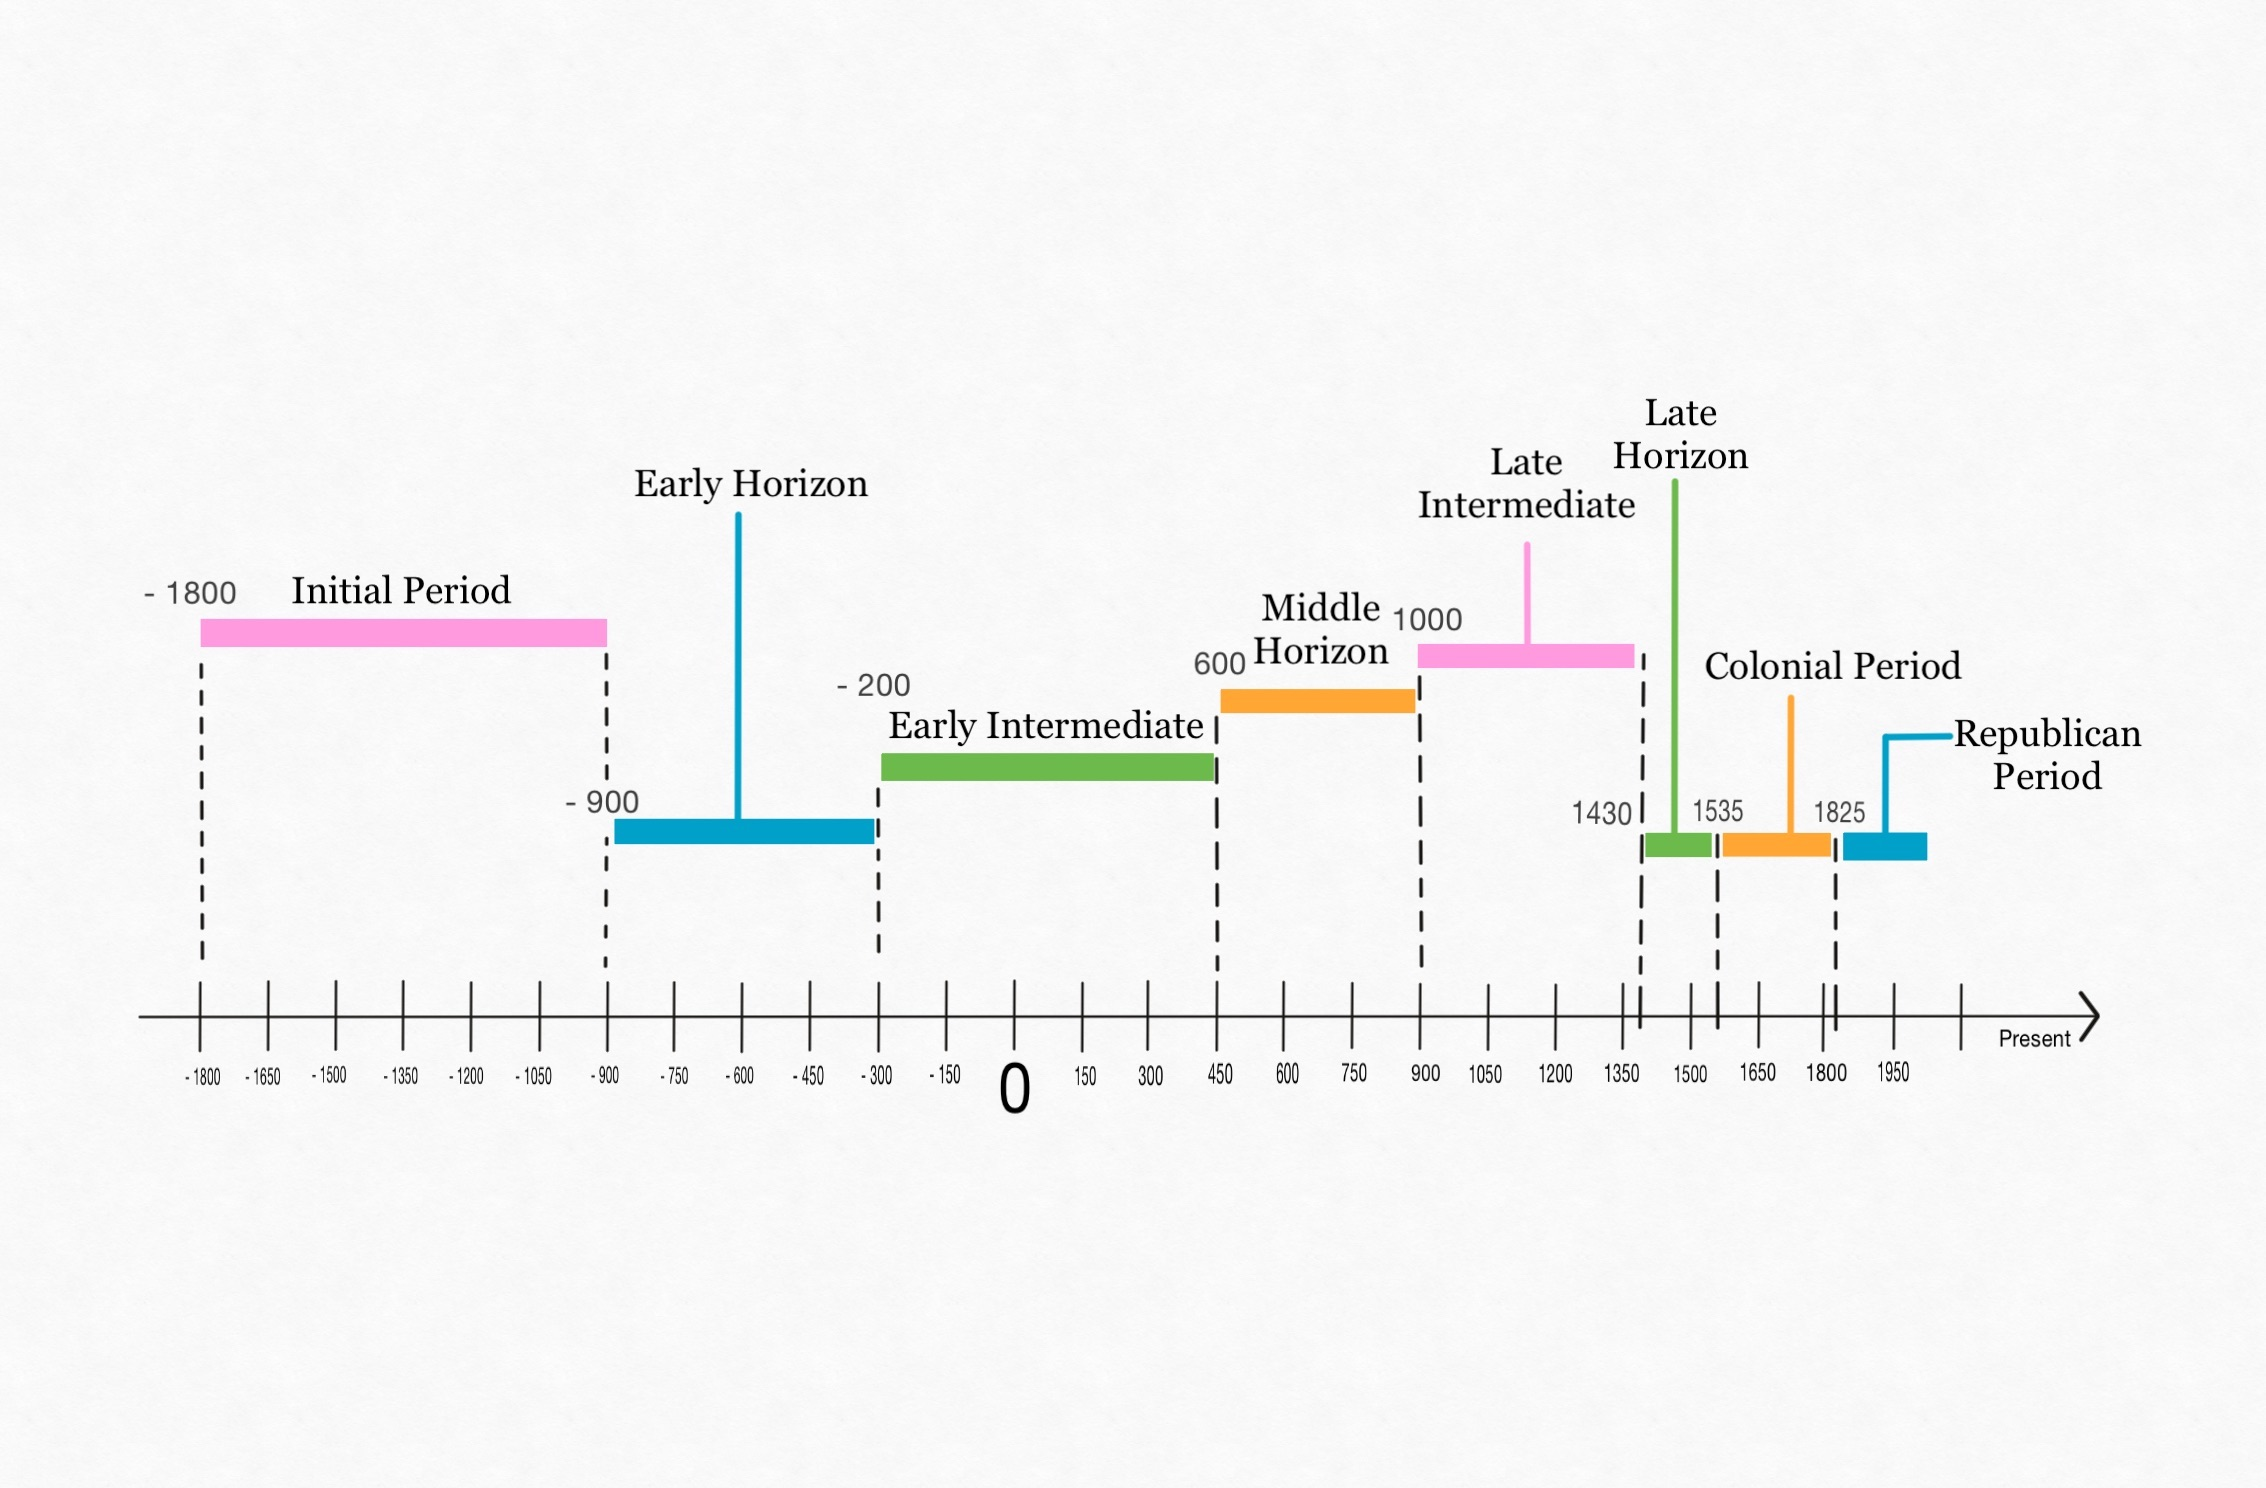
\includegraphics[width=15cm]{../images/FriseChronologique2.jpg}
           	 \caption{Frise chronologique représentant les données temporelles de la base de données après modification}
           	 \label{frisechronofinale}
	 \end{center}
  \end{figure}
  
Cette périodisation nous permettra ensuite d'avoir une approche diachronique des données. Cependant, nous ne devons pas perdre de vue que les périodes historiques restent des concepts vastes construits par les archéologues qui n'ont pas le même sens selon la zone des Andes étudiée. C'est pourquoi cette chronologie se doit d'être croisée avec une approche spatiale, complémentaire dans la compréhension des pièces textiles.

\subsubsection{Données géographiques}

Les données géographiques renseignées dans la base de données, sous forme de chaînes de caractères, nécessitent également un pré-traitement. Les deux informations géographiques de la base de données -- le lieu de production et le lieu de découverte -- contiennent en effet différents niveaux de granularité. Pour tout les cas complétés, nous disposons du pays. Pour d'autres, nous disposons en outre d'une région déterminée par les chercheurs et enfin, parfois, nous disposons d'un lieu précis (nom de village, de province etc.). Pour réaliser un travail de géolocalisation précis, nous avons récupéré pour chaque textile ces trois niveaux de granularité. Par ailleurs, pour les données manquantes, nous avons fait le choix de les encoder en tant que \og Rapa Nui \fg, aussi appelé île de Pâques, puisqu'il s'agit d'une île qui fait partie de la carte du Chili et qui apparaîtra donc lors de la localisation sur les cartes des pays. Son nom, très distinctif, évite également les erreurs de géocodage avec des toponymes similaires ou proches.

  \begin{figure}[!h]
	\begin{center}
		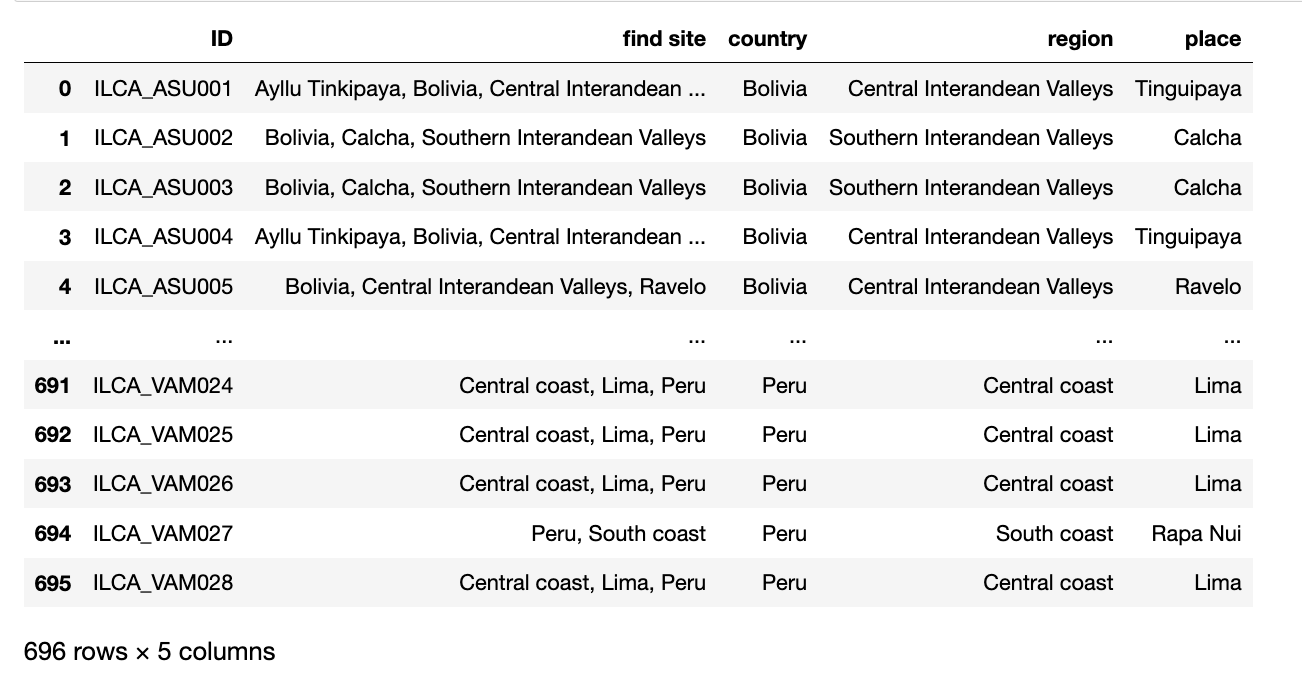
\includegraphics[width=11cm]{../images/geo_df_find.png}
           	 \caption{Tableau avec les trois niveaux de granularité séparés.}
           	 \label{fig:geo_df_find}
	 \end{center}
  \end{figure}
  
  \begin{figure}[!h]
    \begin{minipage}[c]{.5\linewidth}
            \begin{center}
                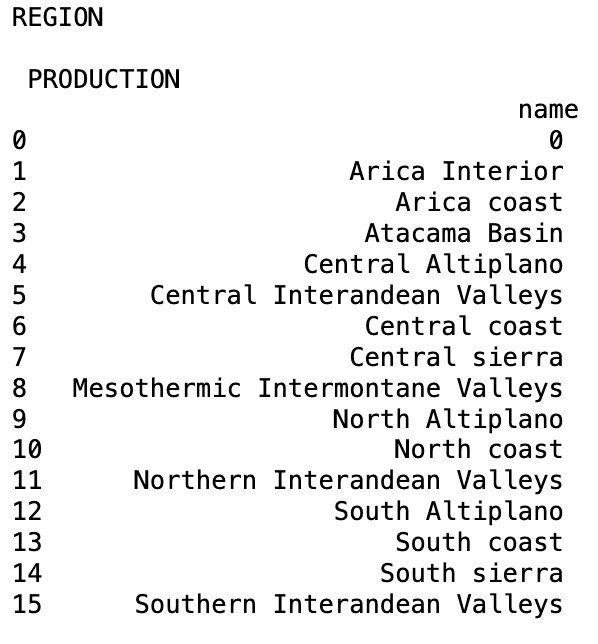
\includegraphics[width=5cm]{../images/regions_orig.png}
            \end{center}
            \caption{Régions originelles.}
            \label{fig:region_orig}   
    \end{minipage}
        \begin{minipage}[c]{.5\linewidth}
        \begin{center}
        		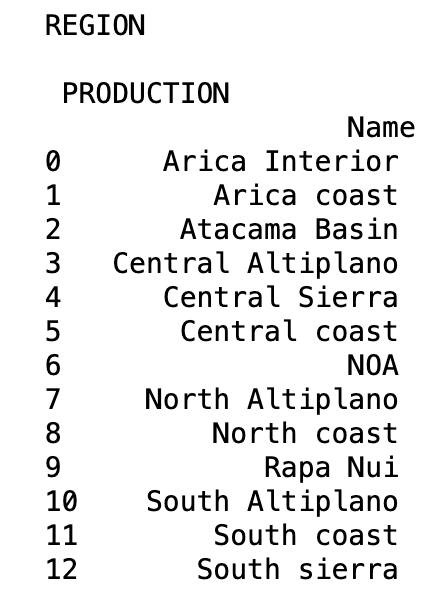
\includegraphics[width=4cm]{../images/regions_fin.png}
	\end{center}
	\caption{Régions finales.}
	\label{fig:region_fin}   
    \end{minipage}
\end{figure}
  
 Toutefois, les informations régionales -- qui sont les plus intéressantes puisque disponibles pour la plupart des textiles, avec une granularité plus importante que les pays -- ne sont pas standardisées et se recouvrent les unes les autres. À partir d'une première exploration, en localisant quelques noms de villages de la base de données dans Google Maps, nous observons cette superposition de certaines régions, comme le montre les images suivantes.
 
 \clearpage
 
   \begin{figure}[!h]
    \begin{minipage}[c]{.5\linewidth}
            \begin{center}
                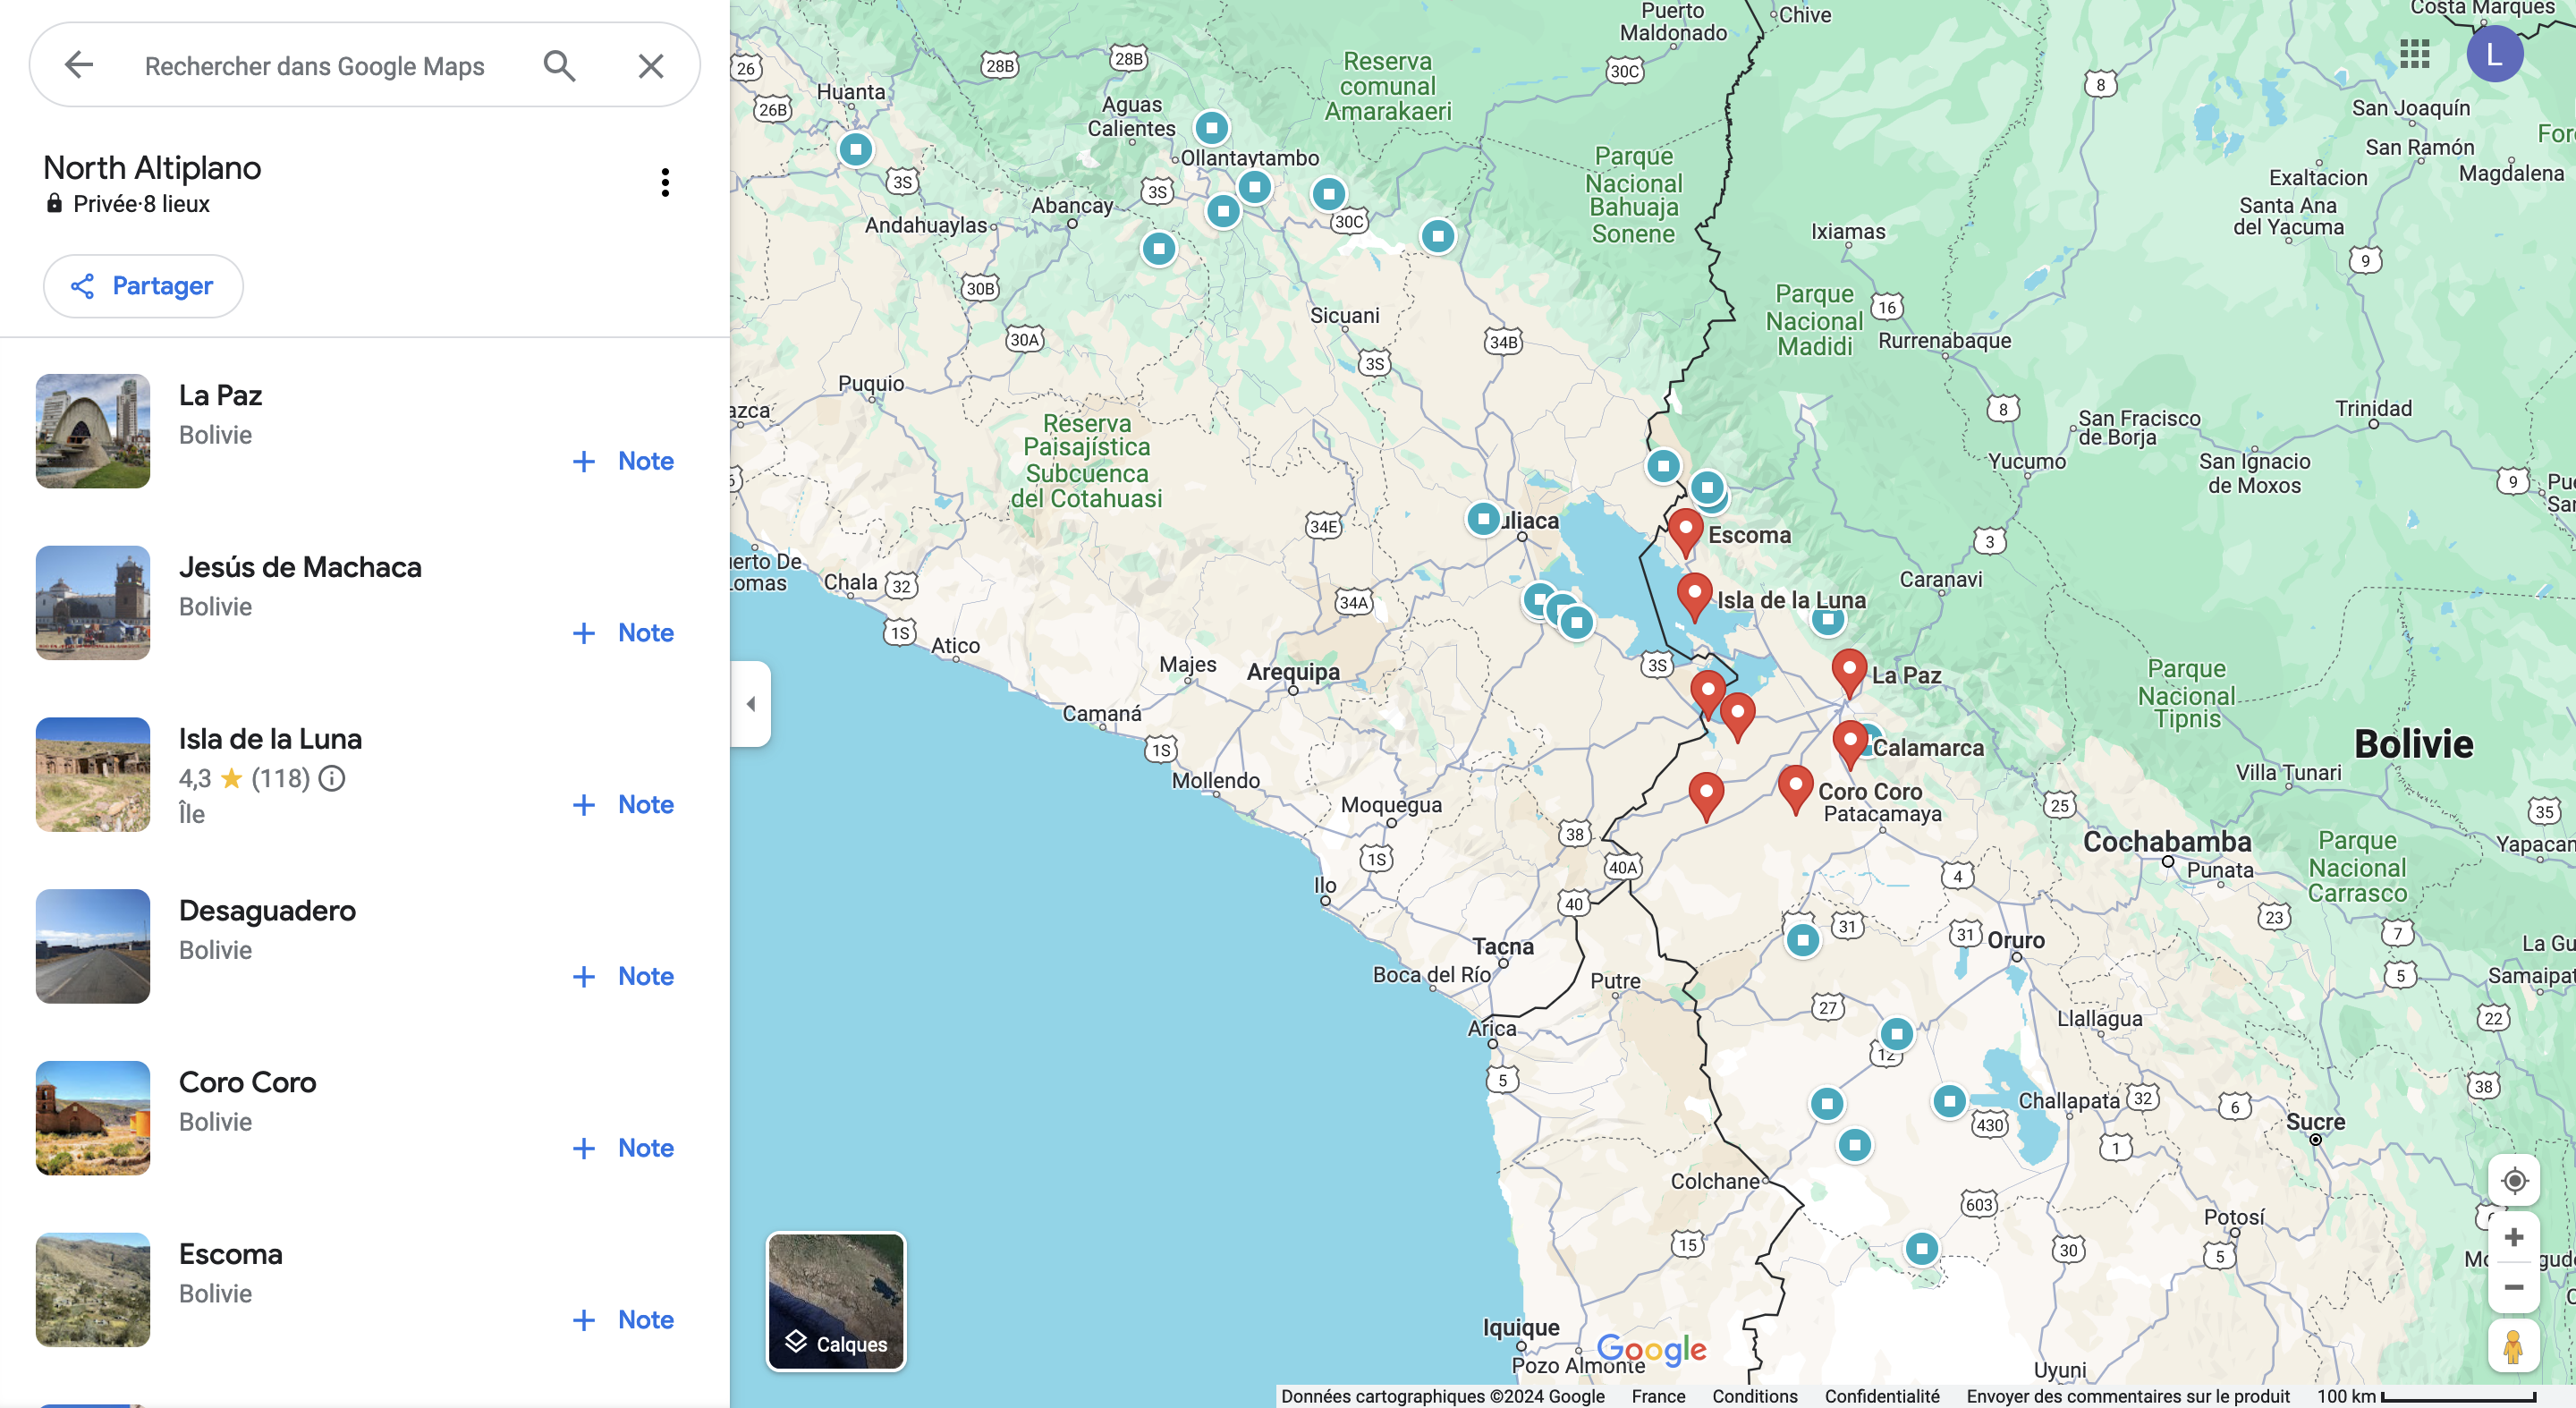
\includegraphics[width=8cm]{../images/GM_NorthAltiplano.png}
            \end{center}
    \end{minipage}
        \begin{minipage}[c]{.5\linewidth}
        \begin{center}
        		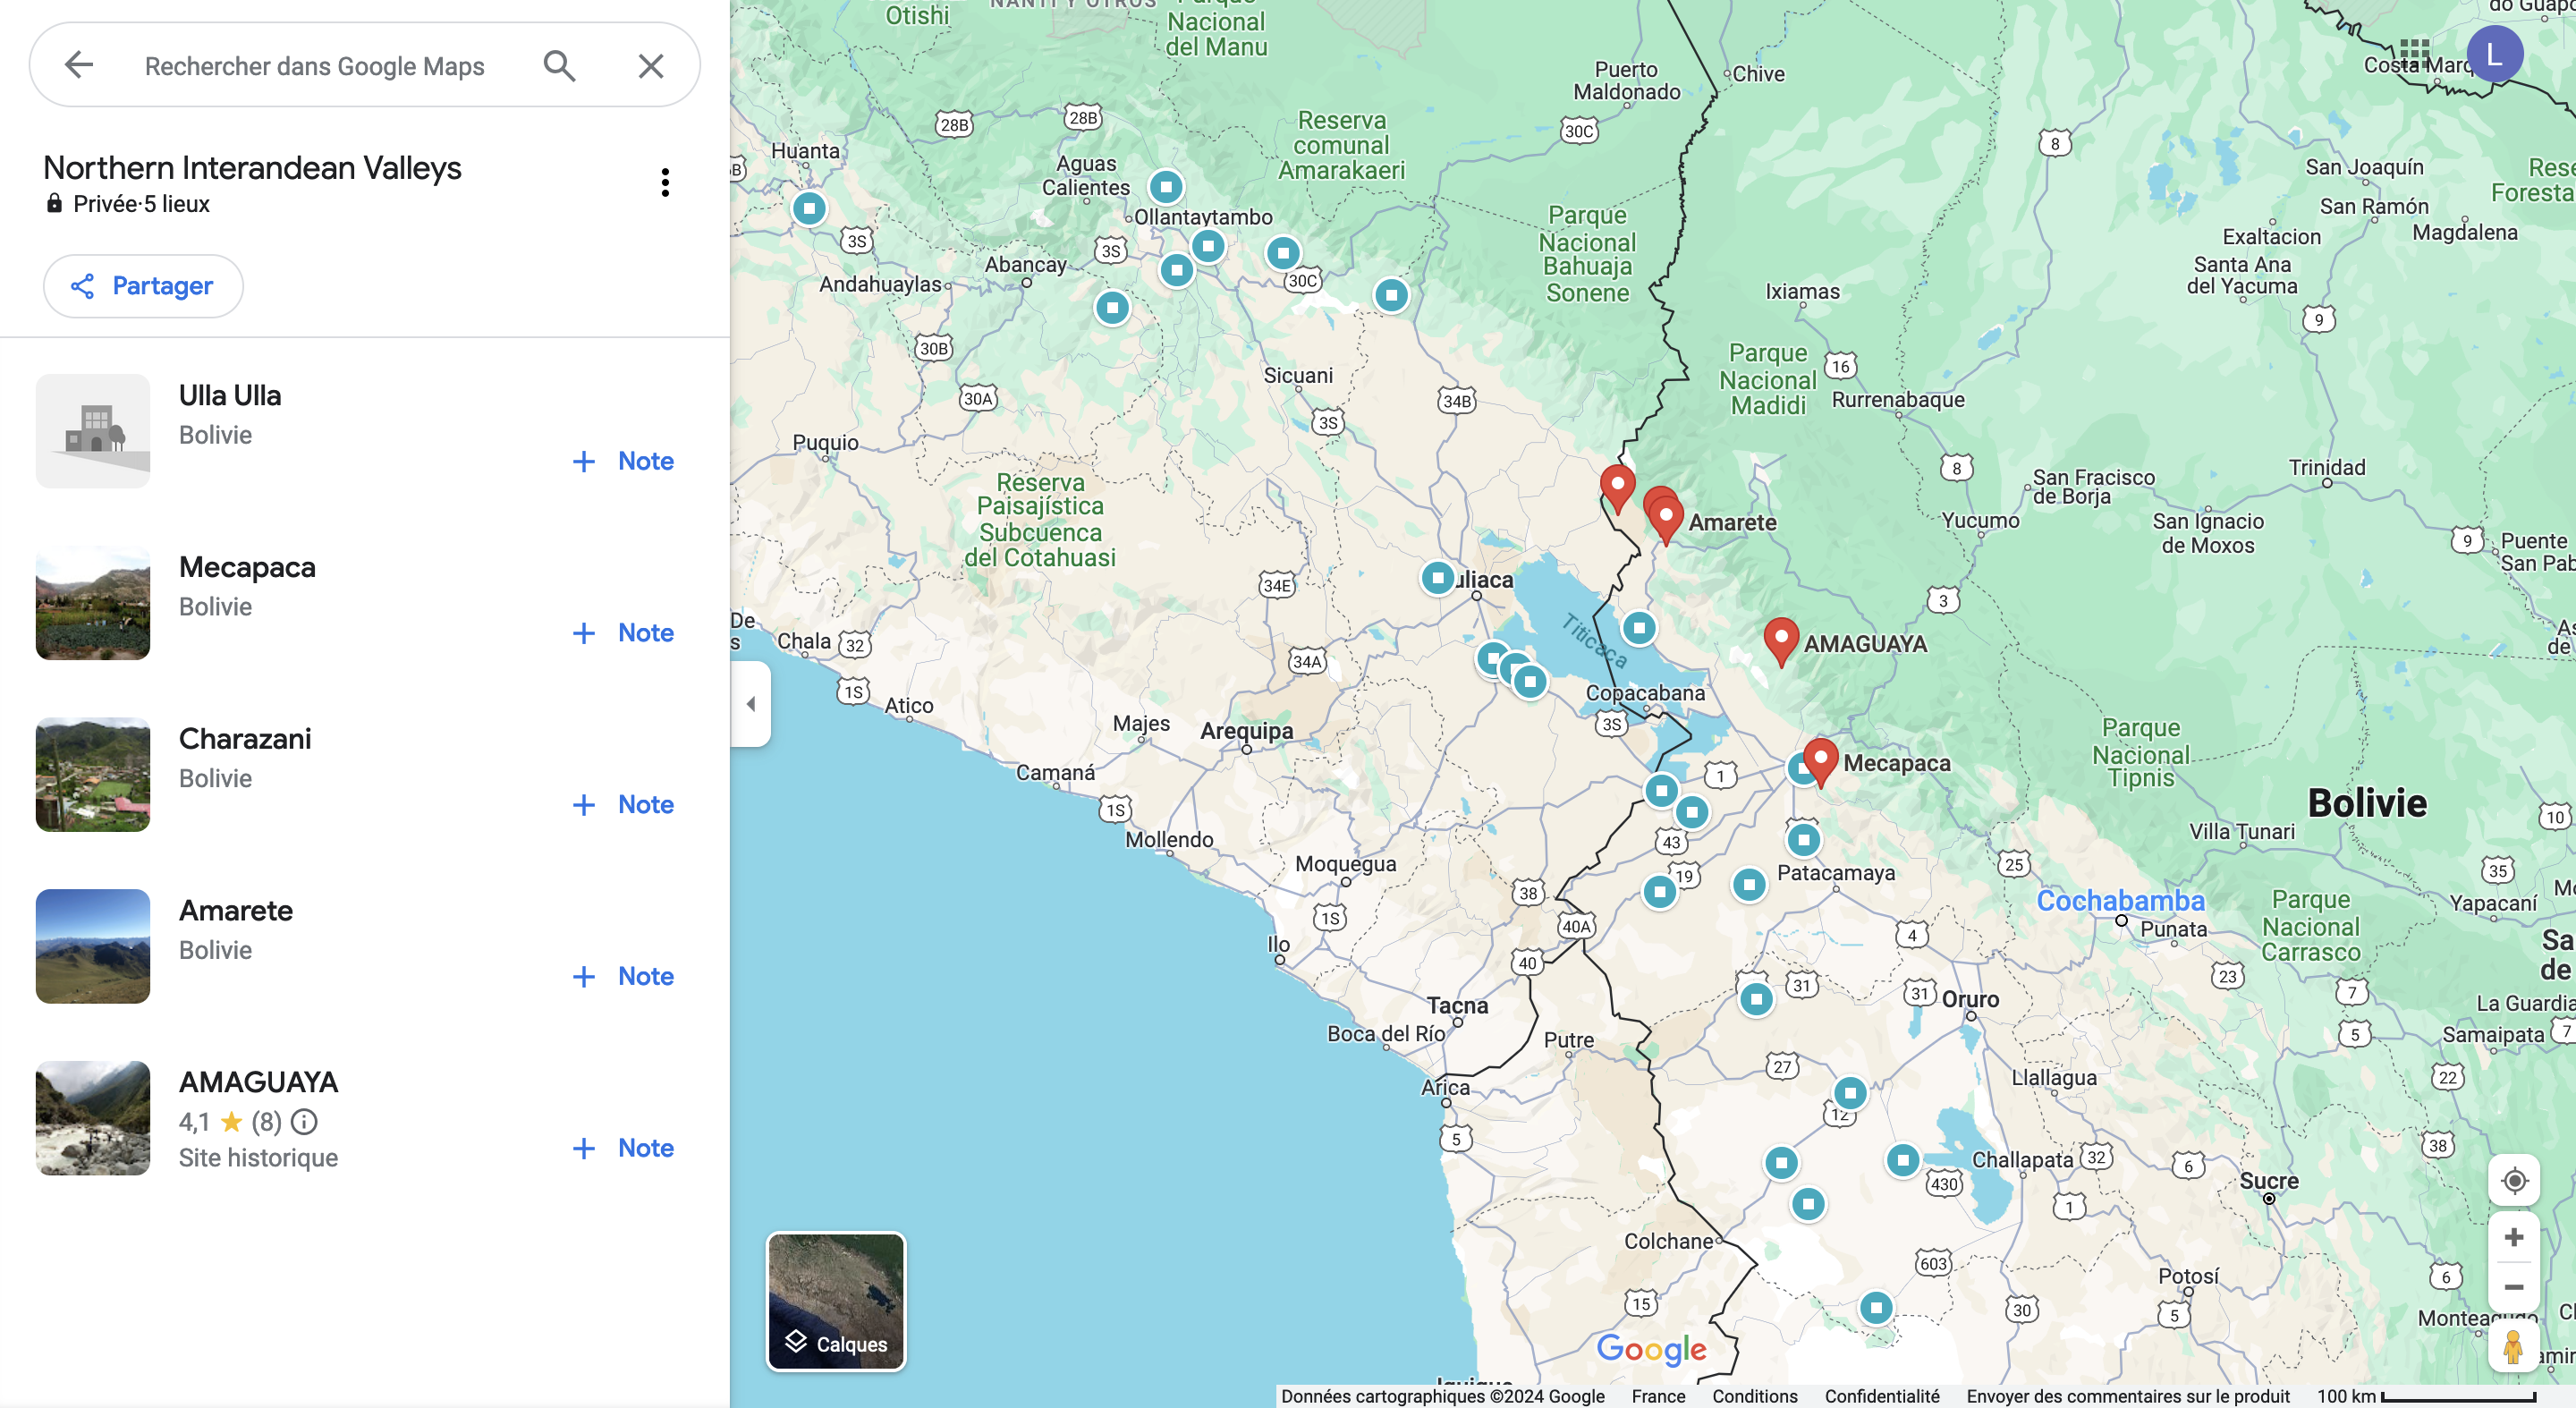
\includegraphics[width=8cm]{../images/GM_NorthernInterandeanValleys.png}
	\end{center}
    \end{minipage}
    	\caption{Captures d'écran de certains points des zones \og North Altiplano \fg \:et \og Northern Interandean Valleys \fg dans Google Maps.}
	\label{fig:GM}   
\end{figure}

Pour remédier à cela, nous avons fait le choix de réduire le nombre de régions de 15 à 12. Les régions qui contiennent le terme \og \textit{Interandean} \fg \:désignent les vallées à l'Est des hauts plateaux boliviens et péruviens (voir le tableau \ref{fig:region_orig}). Nous avons fait le choix de les associer aux zones équivalentes de l'Altiplano. Ce recoupage permet de récupérer des zones d'altitude unifiées d'une part et, d'autre part, des zones côtières. Pour les constituer nous nous sommes appuyés sur le travail de thèse de Romuald Housse en gardant la distinction entre zones péruviennes et boliviennes, présentes dans la base de données. 
 
  \begin{figure}[!h]
	\begin{center}
		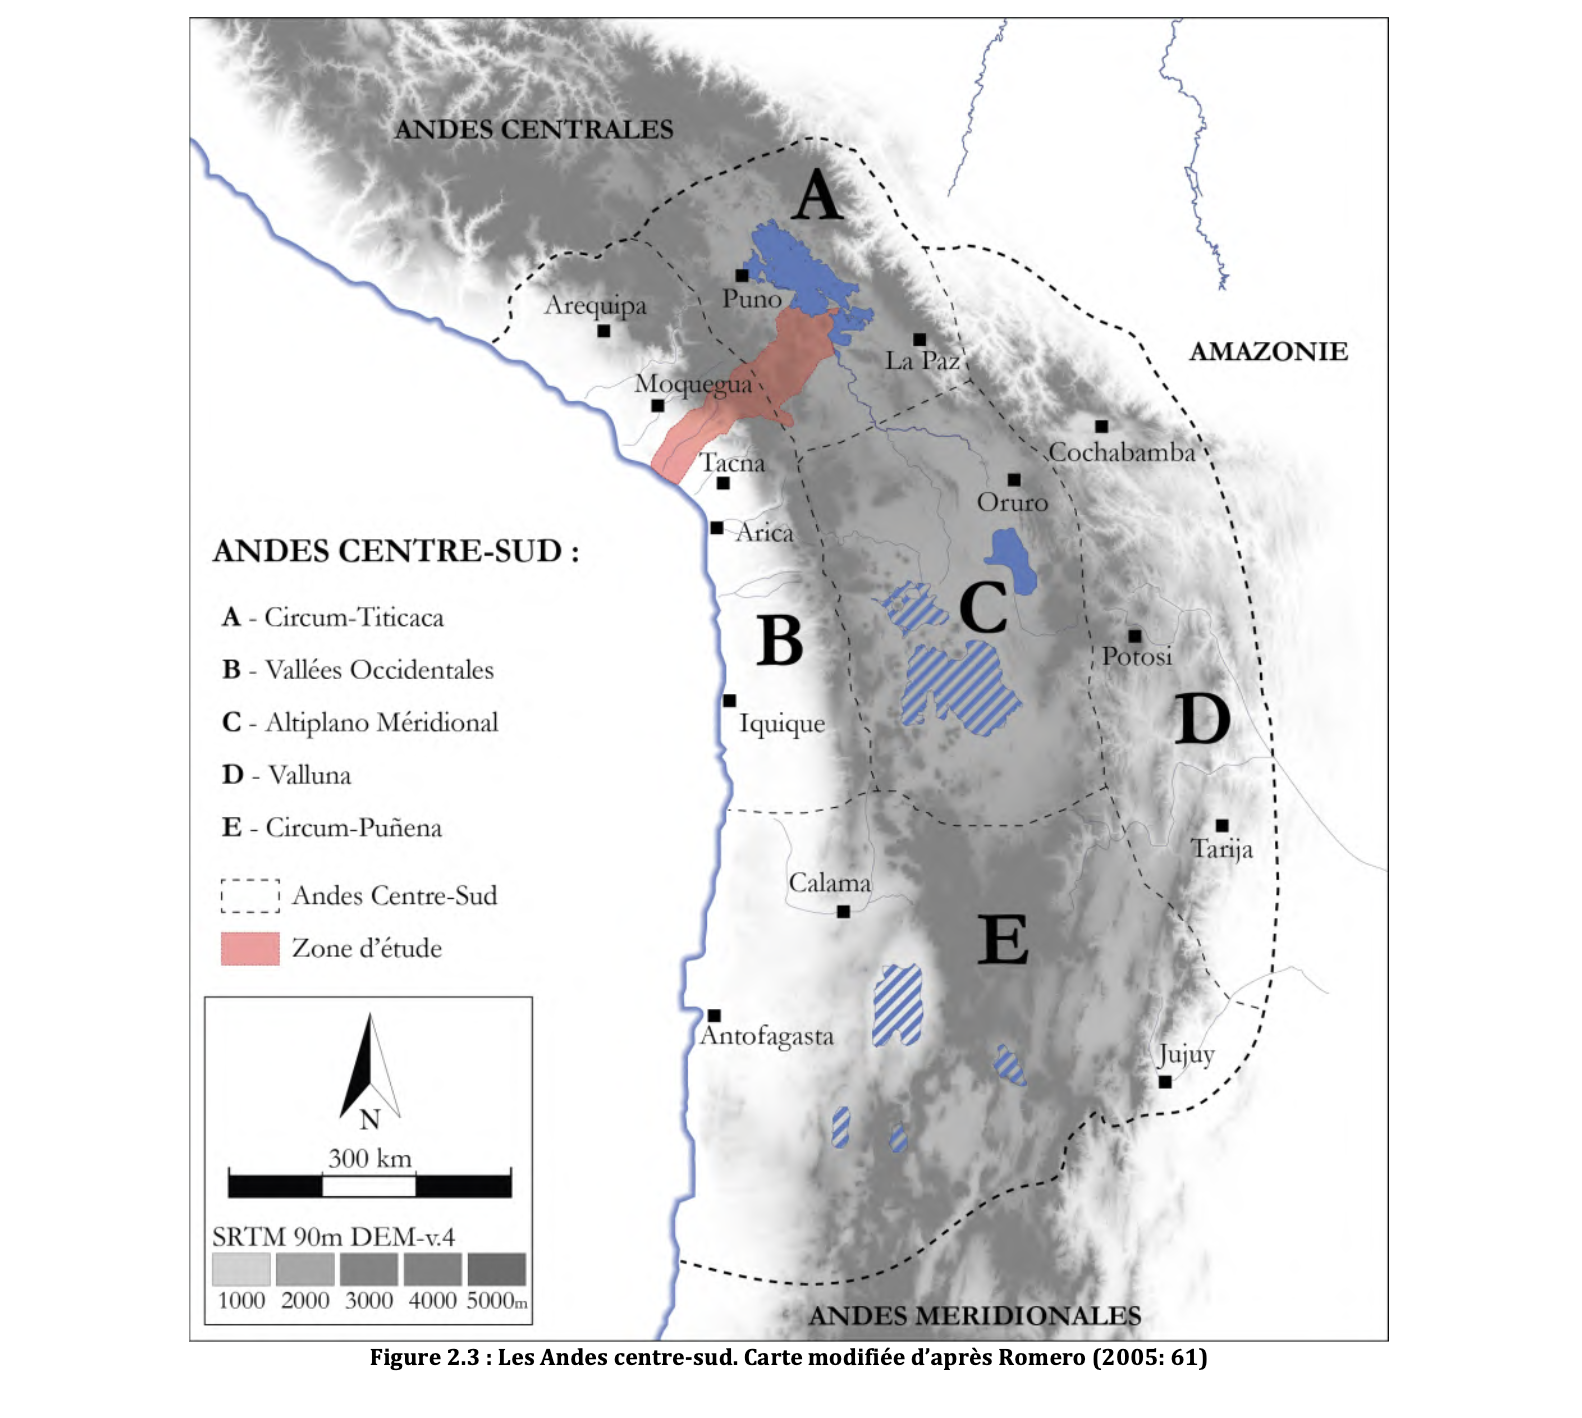
\includegraphics[width=10cm]{../images/mapHOUSSE_2021_p105.png}
           	 \caption{Carte des Andes centre-sud. \\ Source : Housse, 2021, p.~105.}
           	 \label{fig:carteHousse}
	 \end{center}
  \end{figure}

\noindent On obtient les \textbf{régions d'altitudes} suivantes, auxquelles s'ajoutent les régions côtières : 
\begin{itemize}
	\item South sierra (Pérou) : d'Ayacucho au lac Titicaca (inclut les îles péruviennes).
	\item Northern Interandean Valleys + \textbf{North Altiplano} : du lac Titicaca bolivien au nord d'Oruro.
	\item Central Interandean Valleys + \textbf{Central Altiplano} : Altiplano Méridional chez R. Housse, entre Oruro et le lac Poopo.
	\item Southern Interandean Valleys + \textbf{South Altiplano} : Circum-Puñena chez R. Housse mais sans la côte.
\end{itemize}

Après avoir standardisé les régions dans le tableur qui contient les informations de la base de données, nous avons eu recours au logiciel QGIS (logiciel de Système d'Information Géographique libre) pour dessiner et géo-localiser les régions\footnote{Le fichier shapefile contenant les géométrie des régions ainsi que leur localisation se nomme WCP\_region3.shp.}. Nous pouvons observer les régions finales, ainsi que leurs noms, sur la carte suivante.

  \begin{figure}[!h]
	\begin{center}
		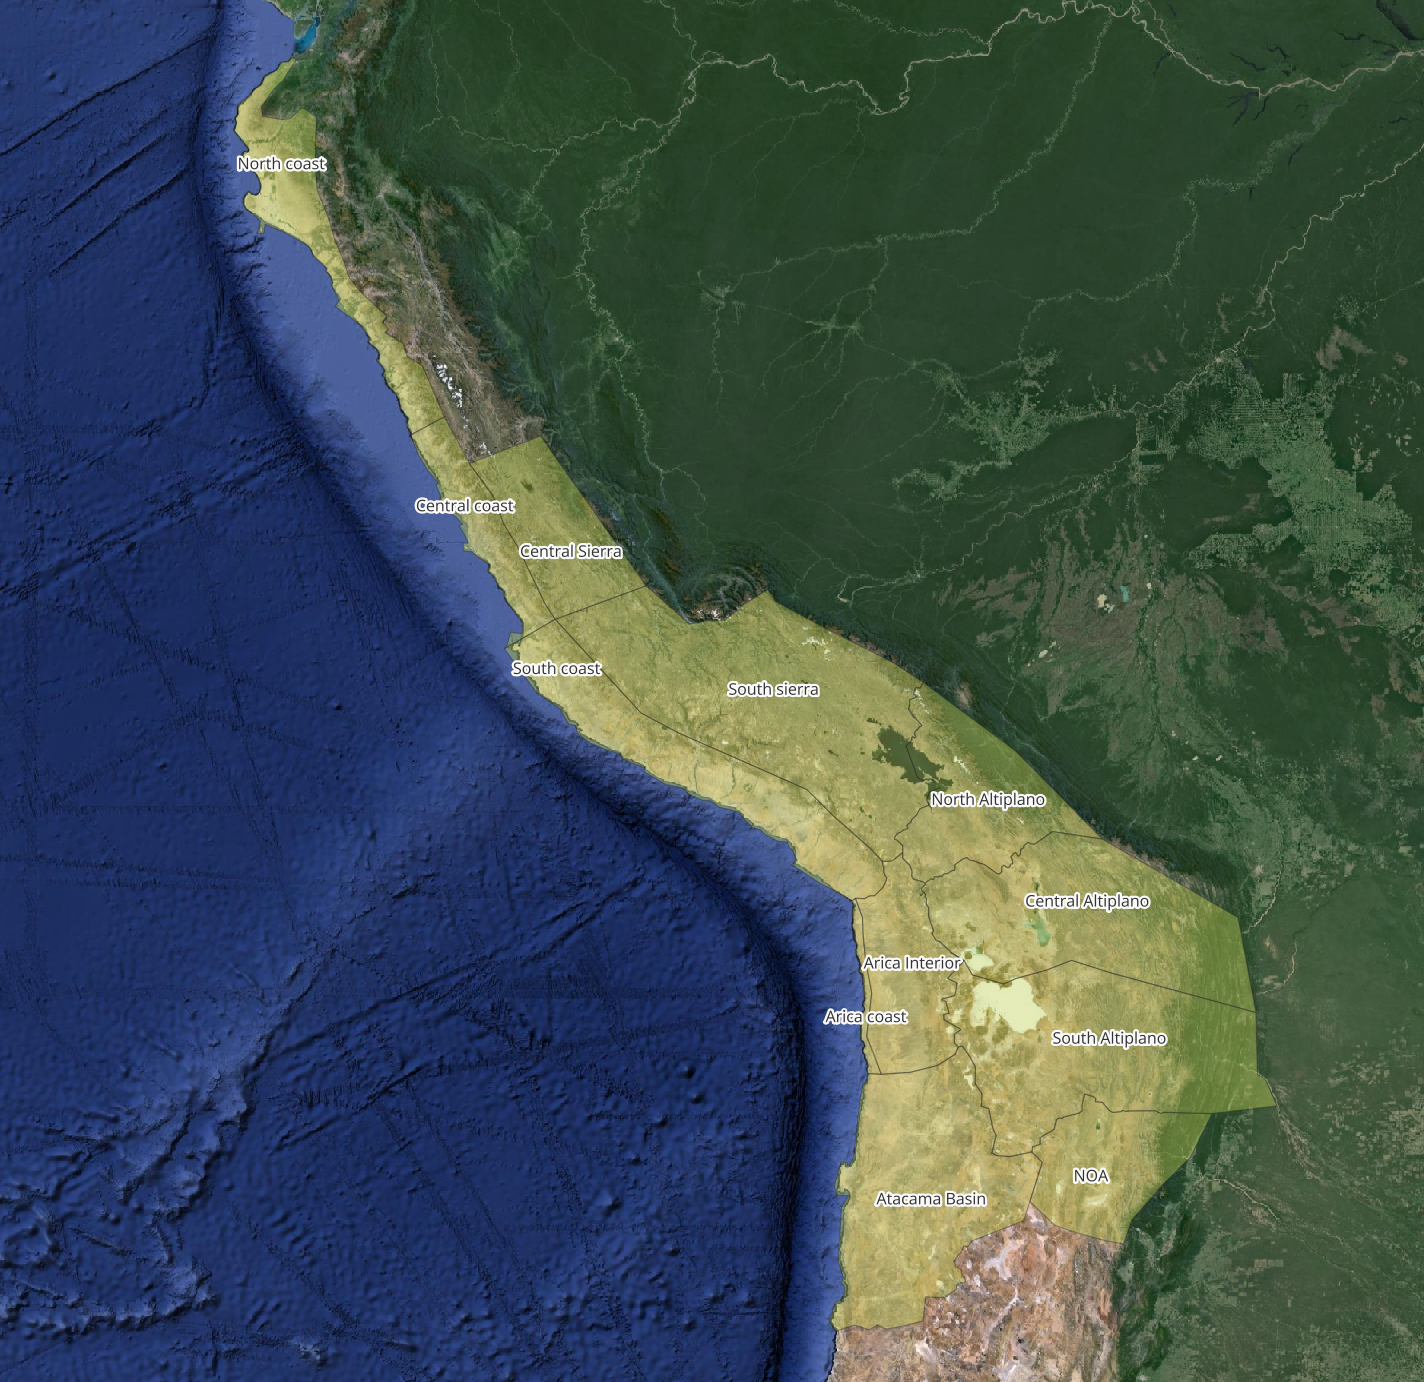
\includegraphics[width=15cm]{../images/region_fin.png}
           	 \caption{Carte des régions finales.}
           	 \label{fig:region}
	 \end{center}
  \end{figure}






\subsection{Premières analyses compréhensives des données}
Après la première phase de pré-traitement et avant de commencer tout travail d'analyse des données, une analyse exploratoire du corpus est nécessaire. À partir de l'ontologie, on peut récupérer les statistiques de chaque valeur dans chaque catégorie et ainsi leur répartition dans la base de données.

Dans le cas des catégories \og repository\fg \:et \og period\fg, c'est-à-dire les lieux de conservation des pièces et les périodes associées à chaque artefact, nous pouvons relever un certain déséquilibre. 
\noindent Les pièces sont réparties entre trois musées principaux : l'\textit{Instituto de Lengua y Cultura Aymara} (La Paz, Bolivie), le \textit{British Museum} (Londres, Royaume-Uni) et le \textit{Museo Nacional de Etnografía y Folklore} (La Paz, Bolivie). La première institution représente plus d'un tiers des pièces disponibles dans la base de données. Cette prépondérance s'explique par la spécificité de l'ILCA, institution partenaire du programme de recherche, dont la collection contient uniquement des textiles ethnographiques et des maquettes de motifs (voir \ref{fig:museum_period}), sa collection contient près de 70\% des textiles de la période républicaine (entre 1825 et aujourd'hui).

\begin{figure}[!h]
            \begin{center}
                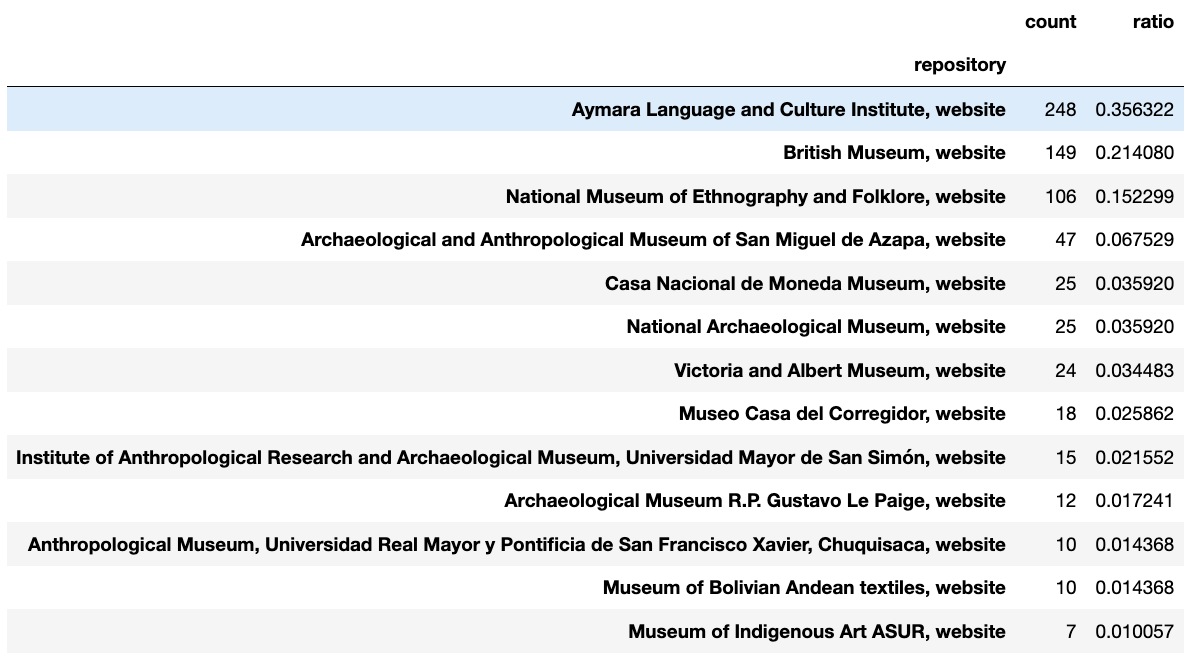
\includegraphics[width=12cm]{../images/count_repository.png}
            \end{center}
    \caption{Décompte des valeurs prises par la catégorie \og repository\fg}     
\end{figure}

\begin{figure}[!h]
        \begin{center}
        		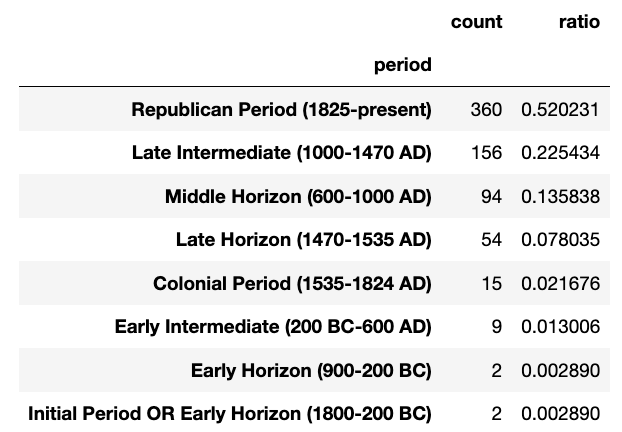
\includegraphics[width=8cm]{../images/count_period}
	\end{center}
    \caption{Décompte des valeurs prises par la catégorie \og period\fg}     
    \label{fig:period}
\end{figure}

Dans le cas de la datation des pièces textiles, la répartition inégale entre les périodes est principalement le fait du choix des experts et des collections auxquelles ils avaient accès. Nous pouvons cependant relever que le nombre de données diminue avec l'ancienneté. La plupart des pièces sont postérieures à la colonisation (375 pièces), et les pièces antérieures se concentrent entre l'Horizon Moyen, la période Intermédiaire Récente et l'Horizon Récent (304 pièces). L'échantillon de textiles disponibles est donc relativement équilibré entre pièces archéologiques d'un côté et pièces historiques et contemporaines de l'autre. Toutefois, plus de 50\% des pièces appartiennent à la période républicaine. Cette prépondérance s'explique notamment par les processus naturels de destruction des textiles. Les périodes les plus anciennes sont ainsi les périodes qui fournissent le moins de textiles.
Dans le cas de la période coloniale et de l'Horizon Récent, plusieurs hypothèses (autre que la sélection réalisée par les chercheurs et chercheuses) peuvent expliquer le nombre plus faible de textiles disponibles. La Conquête (soit la fin de l'Horizon Récent et le début de la période coloniale) est marquée par de nombreux affrontements : les chroniqueurs relatent la destruction volontaire des entrepôts de textiles par les armées incas qui se retiraient devant l'ennemi pour limiter son avancée. Ainsi, John Murra indique que \og L'ennemi [espagnol] n'était pas privé d'hommes (qui, selon Garcilaso, joignaient l'armée européenne) ou de lamas, mais de tissus\footnote{\cite[p.~718]{murraClothItsFunctions1962}. Texte original : \textquotedblleft \textit{The enemy was not deprived of the men (who, according to Garcilaso, joined the European army) or of llamas, but of cloth.}\textquotedblright}.\fg \:Ces témoignages expliquent une partie de la disparition des pièces textiles de cette période, même si une grande quantité de pièces a survécu et se trouve dans les collections de musées qui n'appartiennent pas à notre base de données\footnote{Par exemple, le musée du textile précolombien Amano (Lima), le musée Inka (Cuzco), le musée Larco (Lima)...}. Suite à la Conquête, les espagnols implantent les \textit{obrajes} et développent un nouveau système de production textile pour les populations indigènes. L'apparition de ces manufactures textiles et les différentes lois de la métropole espagnole interdisant certaines pratiques vestimentaires n'impliquent pas la disparition des pratiques textiles pré-coloniales\footnote{\cite[par.~3] {desrosiersLogicasTextilesLogicas1997}}. Cependant, n'étant plus intégrés aux pratiques de l'élite, les textiles perdent de leur attrait pour les scientifiques européens et sont donc plus rarement conservés. L'intérêt pour ces textiles reprend au \siecle{xxi} c'est-à-dire à la période républicaine dans notre chronologie. Par ailleurs, les textiles sélectionnés pour la base de données sont des textiles andins, catégorie qui ne prend pas en compte les textiles produits en grande quantité dans les \textit{obrajes}. 
D'après ce que nous savons, il n'existe pas d'enquête statistique exhaustive sur la quantité de textiles archéologiques disponibles pour la région andine. Techniquement, ces variations dans la répartition posent problème. En effet, les méthodes d'intelligence artificielle nécessitent des corpus d'entraînement équilibrés, avec le même nombre d'éléments par classe (ici, par période), sinon les algorithmes ont tendance à sur-classifier dans les classes prépondérantes de l'échantillon.

 \begin{figure}[!h]
        \begin{center}
        		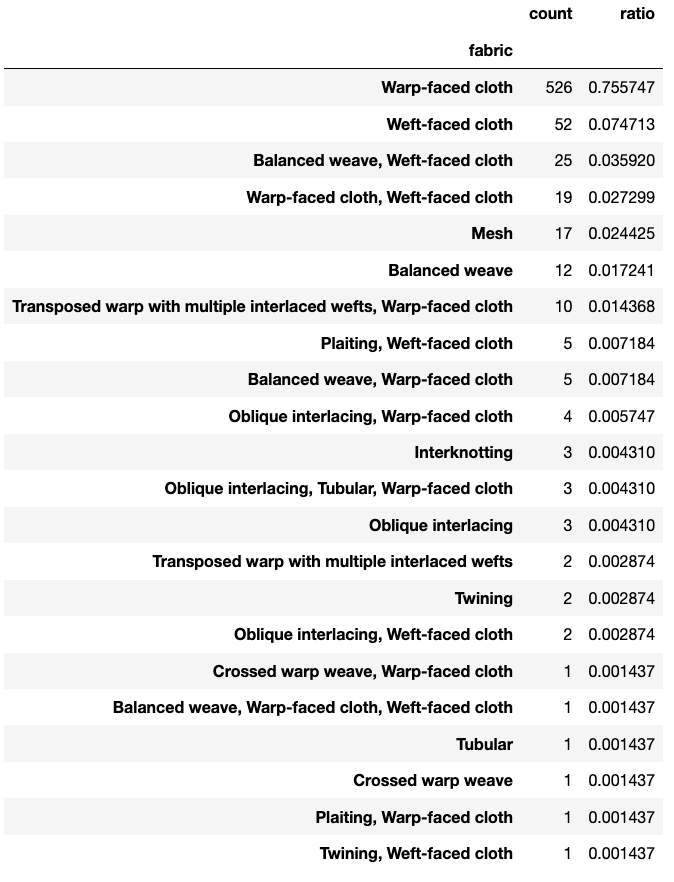
\includegraphics[width=9cm]{../images/count_fabric.png}
	\end{center}
    \caption{Décompte des valeurs prises par la catégorie \og fabric\fg}     
    \label{fig:fabric}
\end{figure}

\clearpage

Nous pouvons aussi nous intéresser aux caractéristiques techniques des pièces textiles. La base de données contient la plupart des structures textiles découvertes dans les Andes\footnote{Voir \cite{harcourtTextilesAnciensPerou2008}.} : toile (\textit{balanced weave}), tissage face chaîne (\textit{warp-faced cloth}), tissage face trame ou tapisserie (\textit{weft-faced cloth}), double étoffe (\textit{double cloth} ou \textit{twining}), réseau (en mailles, \textit{mesh}, ou noué, \textit{interknotting}) et tresse (\textit{plaiting}). 
Là aussi la base de données est déséquilibrée, les tissages face chaîne sont sur-représentés, composant 75,57\% du corpus. Cette sur-représentation va de pair avec la prédominance des pièces contemporaines. Ces textiles contemporains viennent en effet principalement des hautes-terres (voir \ref{fig:place_period}) où le tissage à face chaîne est dominant, et ce sur la longue durée. \\

Ces tableaux nous permettent donc d'obtenir la répartition des métadonnées textiles\footnote{Le reste des tableaux disponibles se trouve en annexe.}. Nous avons ainsi une idée des valeurs disponibles pour chaque catégorie mais il est aussi important de se questionner sur l'influence mutuelle de ces catégories. Pour cela, nous pouvons représenter graphiquement les variables les unes par rapport aux autres afin de voir si des tendances apparaissent. Ces représentations graphiques sont fonctionnelles uniquement pour les catégories qui ont un nombre de valeurs raisonnables. 
Nous analysons ci-dessous plusieurs cas intéressants, soit parce qu'ils illustrent un trait caractéristique de notre \textit{dataset} ou bien parce qu'ils concernent les données que nous mobiliserons dans la suite de ce travail.

 
 \begin{figure}[!h]
	\begin{center}
		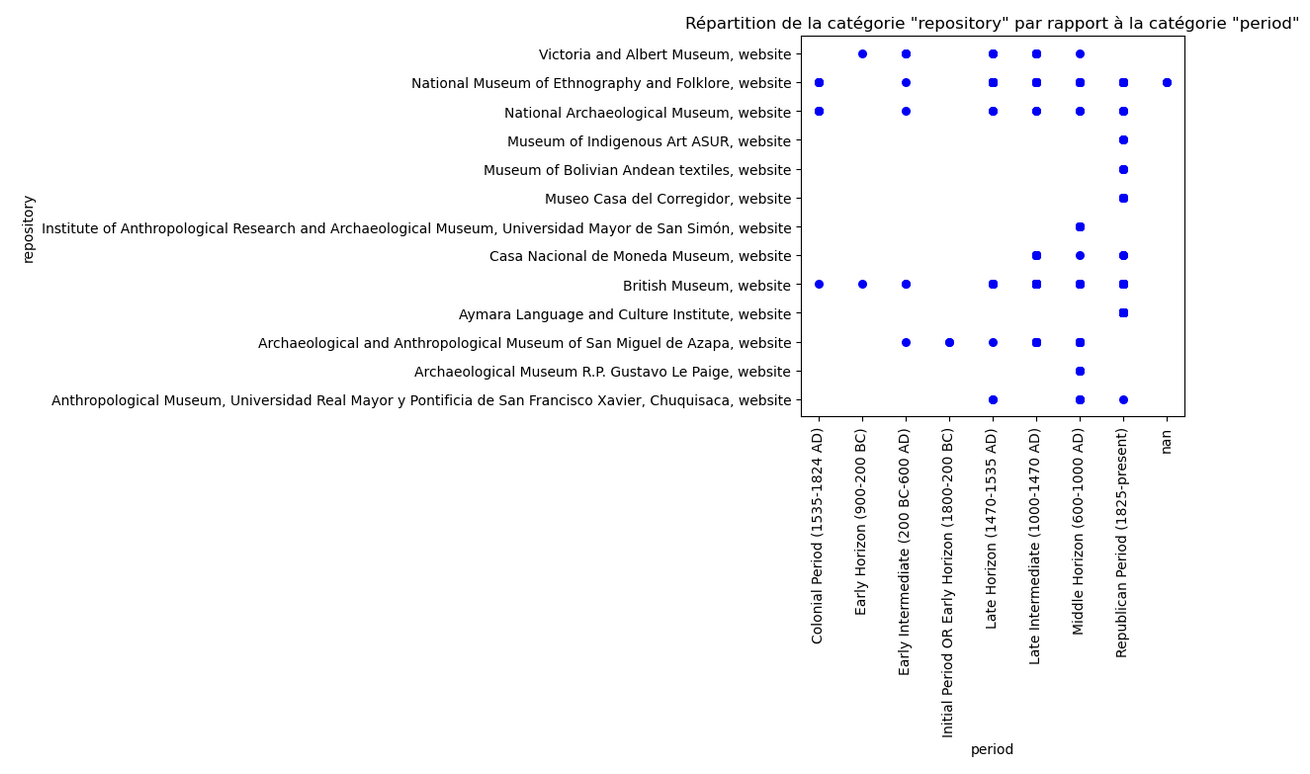
\includegraphics[width=16cm]{../images/R_period_repository.png}
		\caption{Répartition des valeurs possibles prises par es pièces textiles pour les catégories musées et périodes}
		\label{fig:museum_period}
	 \end{center}
\end{figure}

Cette analyse est particulièrement éclairante pour comprendre comment les textiles sont répartis entre les différents musées.  Comme nous l'avons vu la collection issue de l'\textit{Instituto de Lengua y Cultura Aymara} contient uniquement des pièces récentes (période républicaine). Il en est de même pour le \textit{Museo de Arte Indigena} (Sucre, Bolivie), le \textit{Museo de Textiles Andinos Bolivianos} (La Paz, Bolivie) et le \textit{Museo Casa del Corregidor} (Puno, Pérou) qui détiennent des petites collections. À l'inverse, le \textit{Victoria and Albert Museum} (Londres, Royaume-Uni), l'\textit{Instituto de Investigaciones Antropológicas y Museo Arqueológico} (Cochabamba, Bolivie), le \textit{Museo Arqueológico R. P. Gustavo Le Paige} (San Pedro de Atacama, Chili) et le \textit{Museo Arqueologico San Miguel de Azapa} (San Miguel de Azapa, Chili) ont des collections uniquement pré-hispaniques.

\begin{figure}[!h]
    \begin{minipage}[c]{.5\linewidth}
            \begin{center}
                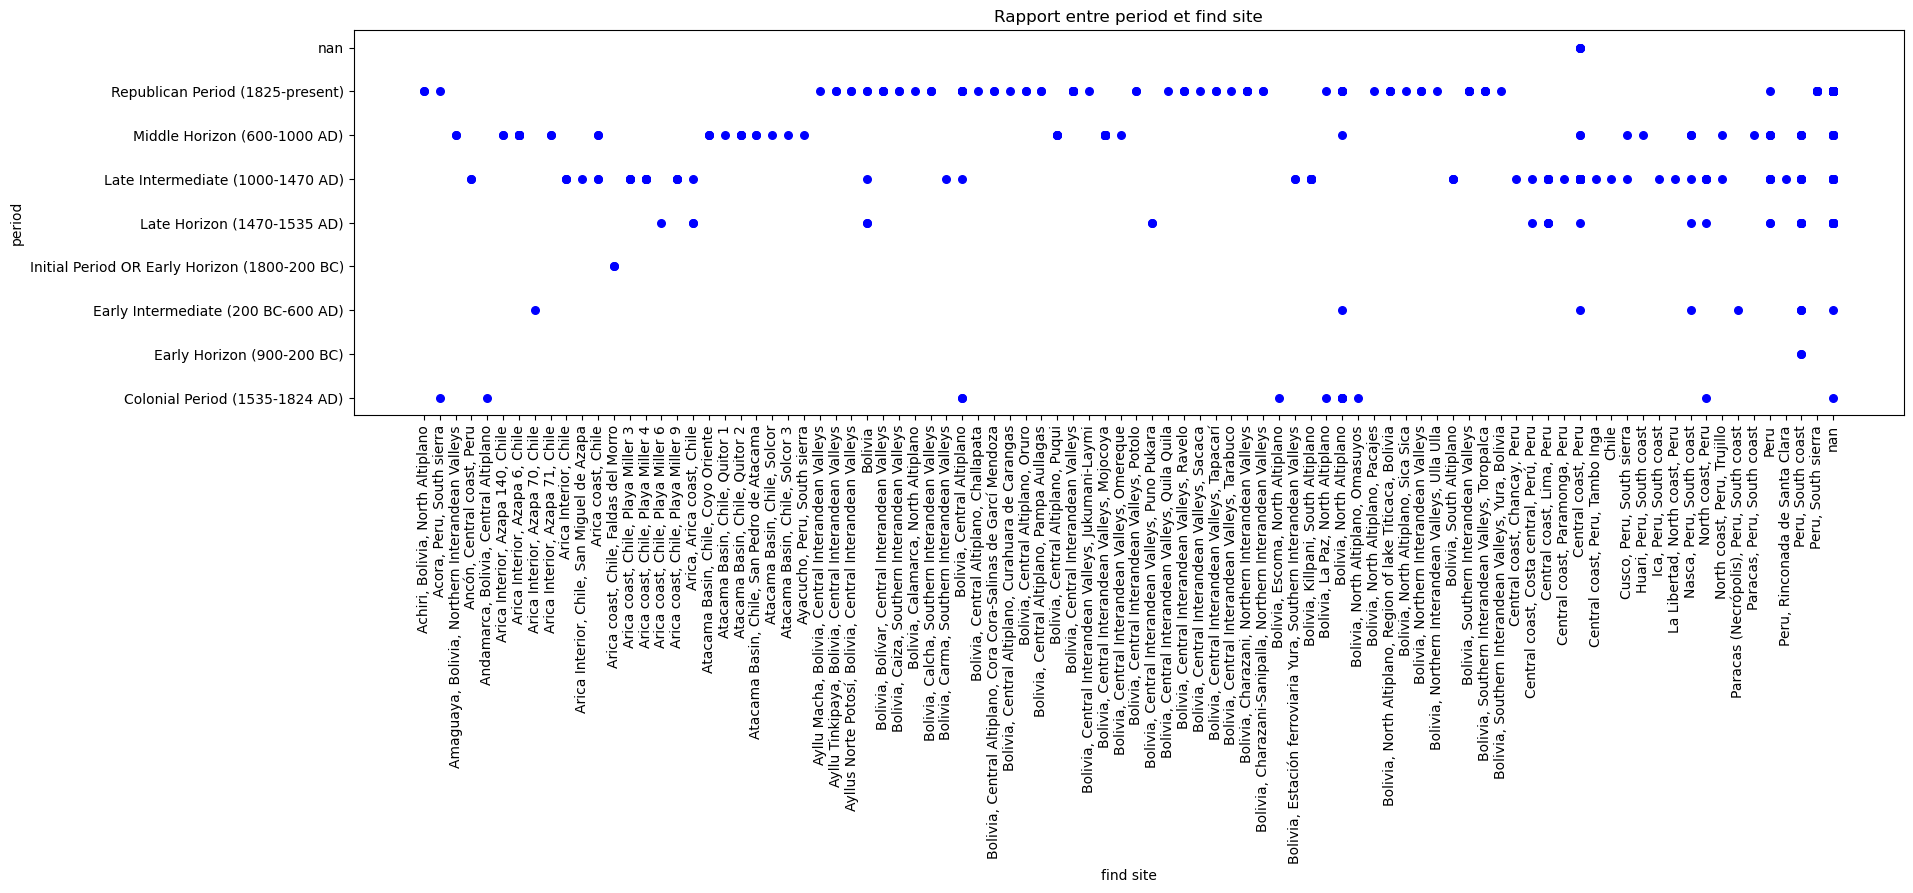
\includegraphics[height=8cm, angle=-90]{../images/R_period_find_site.png}
            \end{center}
    \end{minipage}
        \begin{minipage}[c]{.5\linewidth}
        \begin{center}
        		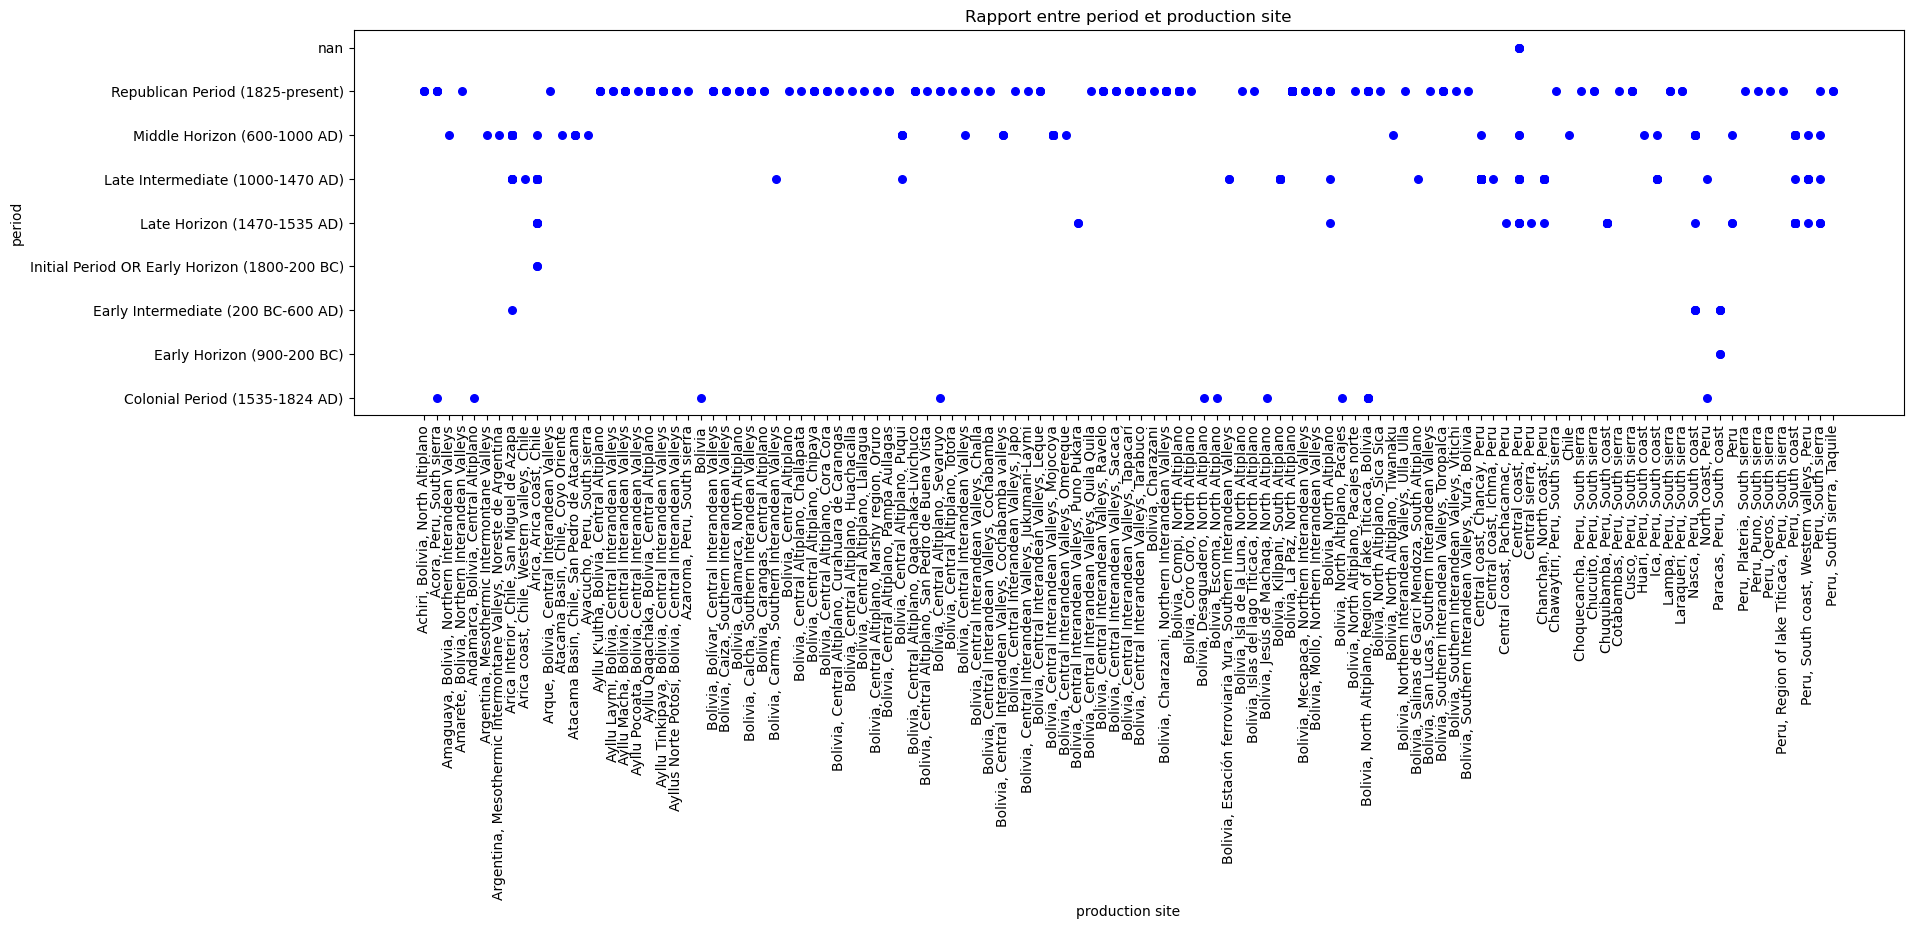
\includegraphics[height=8cm, angle=-90]{../images/R_period_production_site.png}
	\end{center}
    \end{minipage}
    \caption{Répartition des valeurs possibles prises par les pièces textiles pour les catégories période, lieux de découverte et lieux de production}
    \label{fig:place_period}   
\end{figure}
  
À partir du schéma de la répartition des valeurs prises par les pièces textiles pour les catégories périodes et lieux de découverte, nous pouvons observer que la majeure partie des pièces textiles appartiennent aux périodes archéologiques de l'Horizon Moyen (600-1000), de la période intermédiaire tardive (1000-1470) et la période républicaine (1825 - aujourd'hui). Les \textit{clusters} qui se forment sur le graphique nous indiquent la répartition géographique des textiles par période. Ainsi, les textiles de la base de données provenant d'Arica ont été produits sur toutes les périodes exceptée la période contemporaine, la période coloniale et l'Horizon Ancien.
Ceux provenant du désert d'Atacama ont tous été produits au cours de l'Horizon Moyen. Les textiles de la côte centrale péruvienne sont principalement des pièces de l'Intermédiaire Récent et de l'Horizon Récent.
À l'inverse, les pièces contemporaines sont majoritairement issues de Bolivie. Ces répartitions s'expliquent notamment par le contexte de conservation archéologique déjà mentionné. Nous retrouvons quasiment les mêmes répartitions pour les lieux de production.

Ces deux graphiques l'un à côté de l'autre nous permettent de mieux saisir la différence entre les deux catégories géographiques. La catégorie\og lieu de découverte \fg \:indique les lieux d'excavation ou de récupération des pièces textiles, elle est donc composée de plus de textiles archéologiques.
La catégorie \og lieu de production \fg \:contient les informations de production des pièces textiles, c'est-à-dire l'endroit où le textile a été tissé. Il est donc cohérent que cette catégorie contienne plus de textiles contemporains qui sont des textiles qui ont été collectés dans le cadre de recherches ethnographiques bien souvent directement auprès de leur productrice ou de leur producteur.



\section{Traitement des données géographiques}
\subsection{Géocodage des informations géographiques de la base de données}

Après avoir pré-traité les chaînes de caractères des lieux de production et de découverte, nous leur attribuons des coordonnées géographiques, c'est-à-dire une longitude et une latitude\footcite[p.~34]{goldbergTextGeographicCoordinates2007}. Cette méthode de géocodage permet de construire un Système d'Informations Géographiques (ou SIG), c'est-à-dire un ensemble organisé de données spatiales et de données issues des sciences sociales. Nés dans le domaine de la géographie numérique, les SIG se diffusent dans les sciences sociales à partir des années 1970\footnote{\cite[par.~3]{brandoIntroductionHumanitesNumeriques2021}. Voir également le recensement de projets de SIG en histoire et archéologie suivant : \cite{abaranesBibliographieAnalyseSpatiale2021}.}. Aux cartographies se greffent alors les sources iconographiques et textuelles, complétant l'information spatiale.
La base de données contient des données géographiques récentes puisque les chercheurs  ont attribués des lieux contemporains aux textiles et non des lieux historiques. Le processus de géocodage peut donc avoir recours à une base de données géographiques contemporaines. 
Dans ce cas, nous avons eu recours à l'interface de programmation (API) d'Open Street Map, base de données géographique libre et collaborative (sur le modèle de Wikipédia). Nominatim, le géocodeur d'Open Street Map, peut être intégré dans un code en Python auquel on fournit une adresse (plus ou moins précise) et qui nous renvoie des coordonnées géographiques\footnote{Une partie du code utilisée à été extraite de ce tutoriel : visité le 15 décembre 2023, \url{https://medium.com/@amorrison_58444/geocoding-with-the-openstreetmap-api-and-geopy-325633980a15}.}. 

 \begin{figure}[!h]
	\begin{center}
		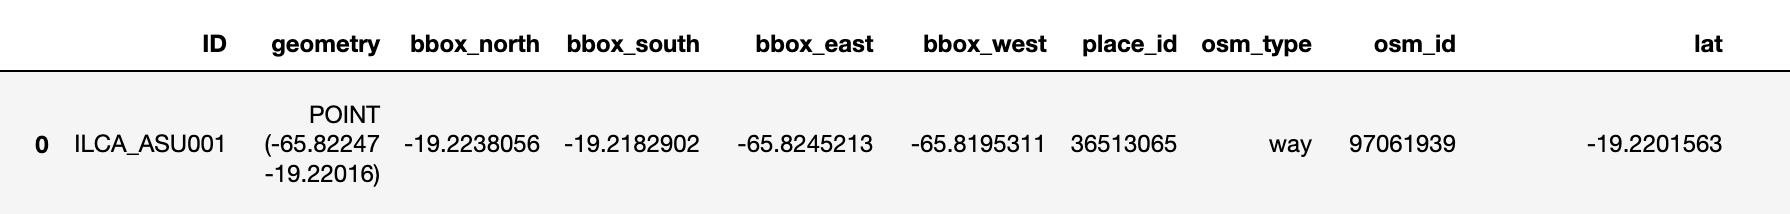
\includegraphics[width=15cm]{../images/gdf_places_prod.png}
	 \end{center}
\end{figure}
 \begin{figure}[!h]
	\begin{center}
		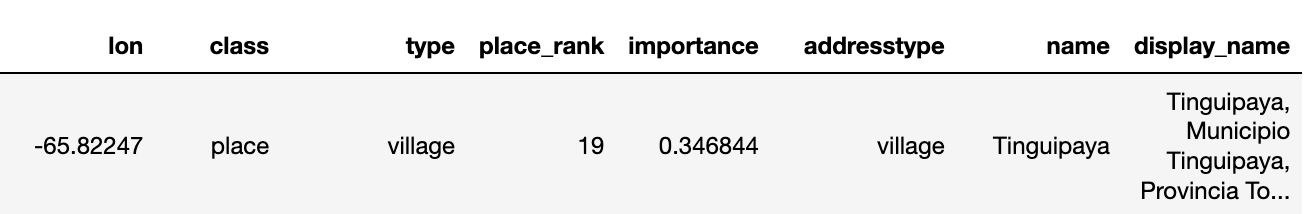
\includegraphics[width=12cm]{../images/gdf_places_prod2.png}
	 \end{center}
	 \caption{Tableau final contenant les identifiants des textiles et les résultats du géocodage.}
	 \label{fig:gdf_places_prod}
\end{figure}

Pour la base de données, les informations géographiques n'étant pas des adresses précises (avec un nom et un numéro de rue), Nominatim nous renvoie plutôt des polygones -- couvrant un périmètre -- que des points précis. Afin de récupérer une latitude et une longitude pour chaque élément, nous récupérons donc le centroïde de chaque polygone et créons une géométrie \og point \fg \:contenant les informations de longitude et de latitude pour chaque textile. Nous réalisons ce processus pour les lieux de production et pour les lieux de découverte. Cette simplification est nécessaire mais pose certains questionnements puisqu'elle implique une perte de précision.

\begin{wrapfigure}{r}{0.4\textwidth}
    \centering
    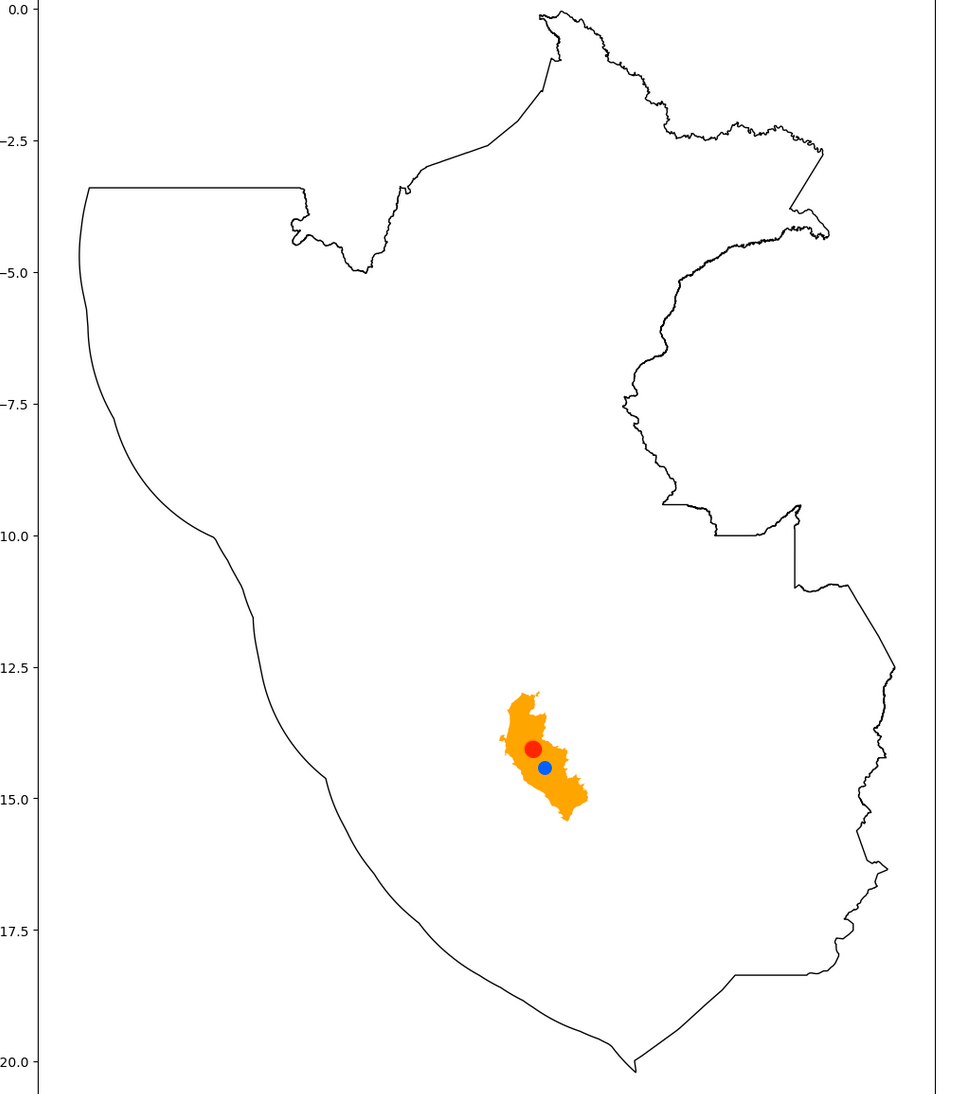
\includegraphics[width=0.4\textwidth]{../images/Ica.png}
    \caption{Géocodage par Open Street Map de la province d'Ica et (centroïde en bleu) et de la ville d'Ica (en rouge).}
    \label{fig:Ica}
\end{wrapfigure}

Les informations géographiques de la base de données étant soit très larges soit très précises, le géocodage n'était pas directement fonctionnel. Les principales difficultés reposaient sur les noms des lieux. Plusieurs toponymes étaient en langues amérindiennes (principalement en aymara ou en quechua), or l'orthographe de ces langues est encore en cours de standardisation. Ainsi, certaines lettres sont interchangeables comme le \og c \fg, le \og k \fg \:et le \og q \fg, ou le \og o \fg \:et le \og u\fg, ou encore le \og i \fg \:et le \og e \fg. Ces variations orthographiques posent problème puisque que Nominatim repose sur l'orthographe des noms pour les trouver dans la base de données d'Open Street Map. Au sein de cette dernière, les variations orthographiques n'apparaissent pas et donc ne sont pas prises en compte au moment du géocodage. Par ailleurs, au Pérou et en Bolivie, il est commun d'avoir le même toponyme pour différents niveaux administratifs, comme nous pouvons le voir sur la figure \ref{fig:Ica}. Une désambiguïsation était donc nécessaire pour ces cas, en spécifiant le niveau administratif du lieu. Enfin, neuf lieux de découvertes textiles étaient des sites archéologiques, pour lesquels une information numérique était accolée au toponyme, référençant la zone précise du site de provenance. Cette information numérique était prise en compte comme une information de numéro de rue par Nominatim qui renvoyait systématiquement une localisation erronée. Ces erreurs ont été modifiées à la main en amont du géocodage et la valeur \og Rapa Nui \fg \:a été associée aux cas irrésolus.


\subsection{Un géocodage robuste ?}
Le processus de géocodage se compose d'allers-retours entre les résultats fournis par l'API d'Open Street Map, les points renseignés sur la carte et les frontières des régions dessinées sur QGIS.

 \begin{figure}[!h]
	\begin{center}
		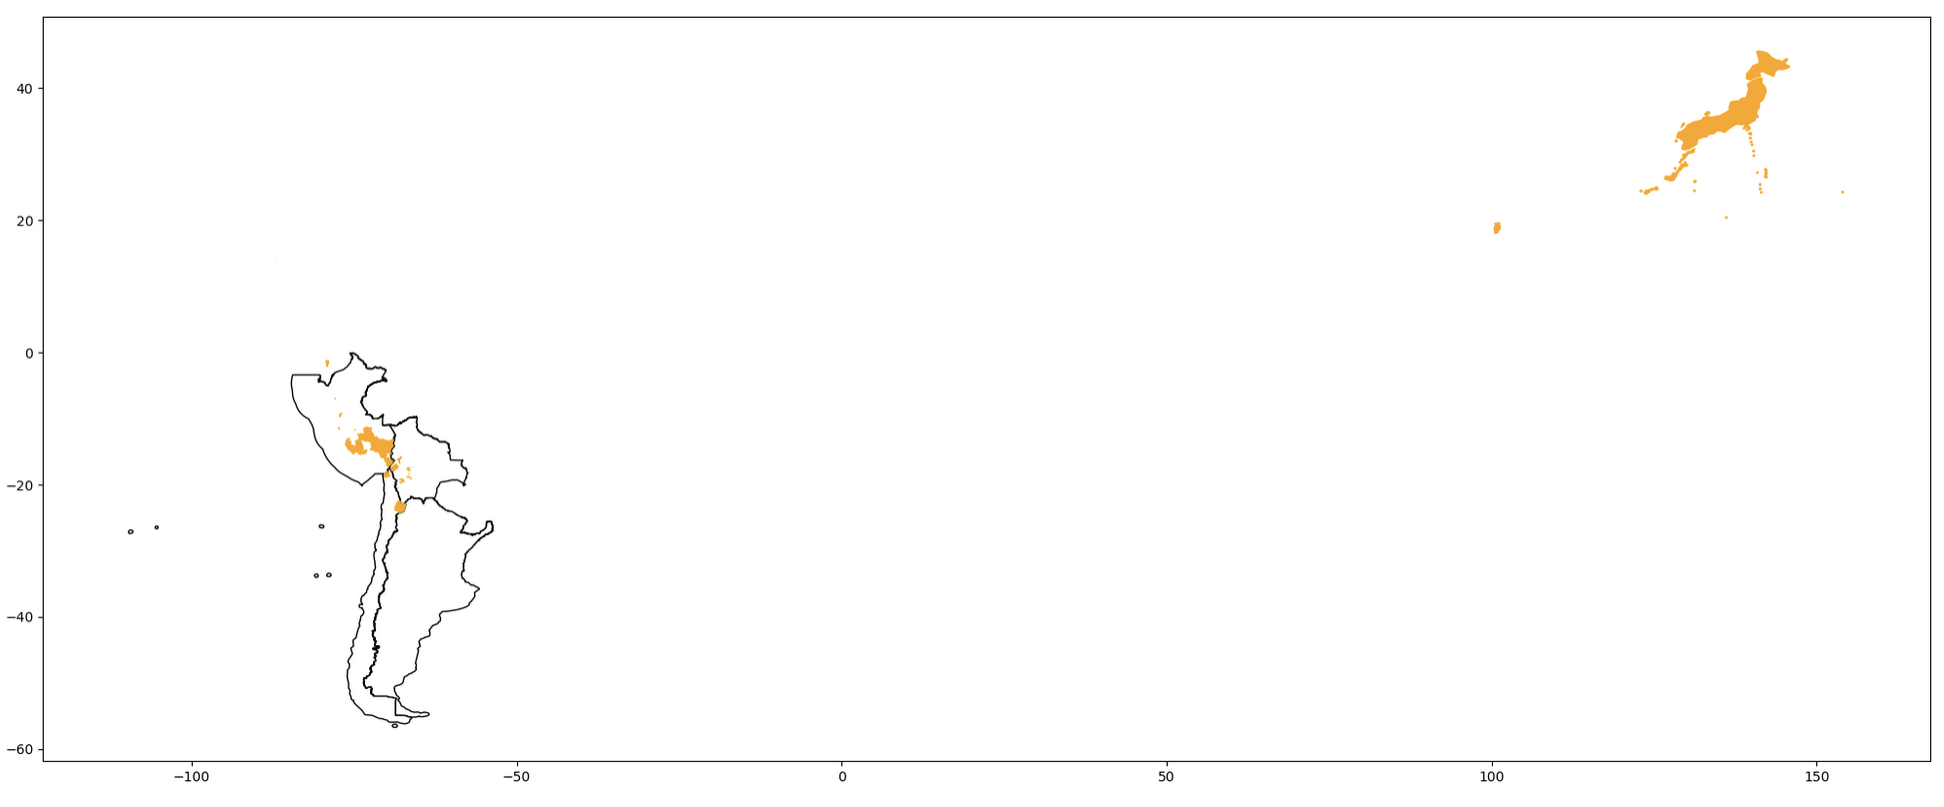
\includegraphics[width=15cm]{../images/erreursGeocodage.png}
		\caption{Première tentative de géocodage.}
		\label{fig:erreurGeocod}
	 \end{center}
\end{figure}

Les premières tentatives étaient infructueuses, comme nous pouvons le voir sur le premier résultat obtenu. L'apparition du Japon sur la carte s'explique par la prise en compte des valeurs nulles -- NaN --  en tant que nom de région japonaise. En remplaçant les valeurs nulles par \og Rapa Nui \fg, nous avons pu réduire le résultat du géocodage à la zone andine. Par ailleurs, en croisant les noms de lieux qui n'étaient pas géoréférencés dans l'API d'Open Street Map avec certaines monographies archéologiques et ethnographiques sur la zone andine, nous avons pu fournir à l'API une approximation du lieu, notamment en fournissant un élément géographique voisin. Par exemple, pour les villages de Jukumani-Laymi et de Laymi, Laurence Charlier Zeineddine qui a fait son terrain dans cette zone nous indique qu'ils ont été regroupés sous le nom de \og Chayanta \fg\footcite[par.~12]{charlierzeineddineChapitreLikIchiri2015}. Il en est de même pour le village de K'ultha que n'arrivait pas à géolocaliser l'API. Denise Y. Arnold et Elvira Espejo indiquent que les villages de Qaqachaka et K'ultha sont voisins\footcite[p.~304]{arnoldWovenTechniquesSocial2014}, ce qui nous a permis. de référencer Qaqachaka et K'ultha avec l'orthographe \og Kaka Chaca \fg \:reconnue par Open Street Map. Toutefois, dans le cas des textiles ethnographiques, se pose la question de l'anonymisation, pratique commune chez les ethnologues pour protéger leurs enquêté\inclusives{e}. Dans le cas de la base de données, il semble que, puisque ce sont les textiles qui sont identifiés, les chercheurs n'ont pas eu recours à une anonymisation géographique, si c'est le cas ils ne l'ont pas spécifiée.
Toutefois, comment être certains que les points géoréférencés sont réellement sur les lieux référencés par les chercheurs ? \\

Face à ces questions, nous avons mis en place un processus automatique de vérification, ou du moins de limitation, des erreurs. Il s'agit de vérifier que les points géocodés sont bien dans les régions associées aux textiles. Tout d'abord, il a fallu mettre de côté les valeurs nulles ou erronées qui ont été indiquées comme \og Rapa Nui \fg \:et pour lesquelles nous savons que le point précis n'est pas dans la région renseignée. Deux cas d'erreurs sont apparus au moment de la vérification : les éléments à la frontières des régions et les éléments ostensiblement mal géocodés. Dans le premier cas, après vérification de la véracité de la localisation des points concernés, nous avons pu redessiner les régions sur QGIS pour qu'elles les incluent. Dans le second cas, c'est à l'étape de géocodage qu'il a fallu modifier le nom fourni, notamment en rajoutant le pays ou le niveau administratif afin de récupérer un point correctement géolocalisé.

Nous obtenons les résultats finaux suivants. La première ligne correspond aux erreurs de géocodage calculées et la seconde à ce même nombre d'erreurs en enlevant les valeurs nulles qui apparaissent comme des erreurs lors de la vérification. Ainsi, nous n'avons aucune erreur pour les lieux de découverte et seulement deux erreurs pour les lieux de production. Ces deux erreurs sont liées à la forme des régions dessinées sur QGIS. La première est sur le Lac Titicaca, en suivant la frontière peruano-bolivienne du lac un des points est situé en Bolivie alors qu'il est renseigné comme péruvien dans la base de données, avec une erreur de moins d'un kilomètre. La seconde erreur n'est pas non plus une erreur de géocodage mais une erreur de frontières régionales. Le point est bien géocodé sur les Salinas de Garcí Mendoza mais il est associé à l'Altiplano Sud dans la base de données alors qu'au vu des autres points, il fait plutôt parti de l'Altiplano Central.

\clearpage
  
 \begin{figure}[!h]
	\begin{center}
		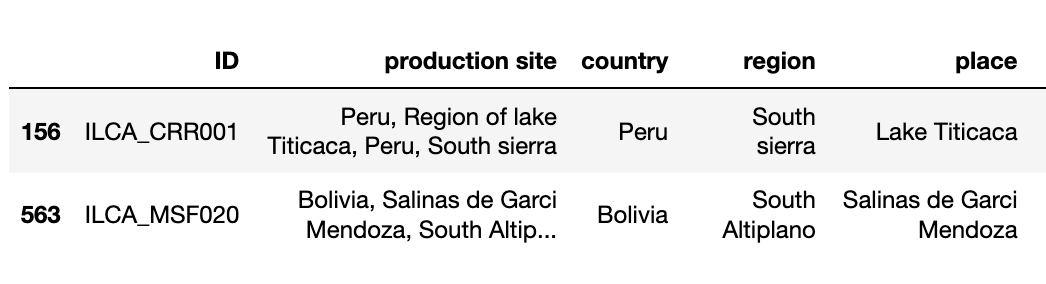
\includegraphics[width=12cm]{../images/verif_prod3bis.png}
		\caption{Erreurs finales pour les lieux de production.}
		\label{fig:erreur_verif}
	 \end{center}
\end{figure}

La vérification du géocodage a eu lieu tout au long du traitement des données. Ainsi, au moment du calcul des distances entre lieu de découverte et lieu de production des textiles, les distances entre les points géocodés correspondent aux lieux présent dans la base de données (voir tableau page \pageref{fig:distancetab}). Une partie de la vérification se fait en restant au plus proche des données initiales pour les confronter aux données géographiques produites lors du géocodage et des analyses suivantes.

\subsection{Cartographier la répartition des textiles de la base de données}

\begin{wrapfigure}{r}{0.4\textwidth}
    \centering
    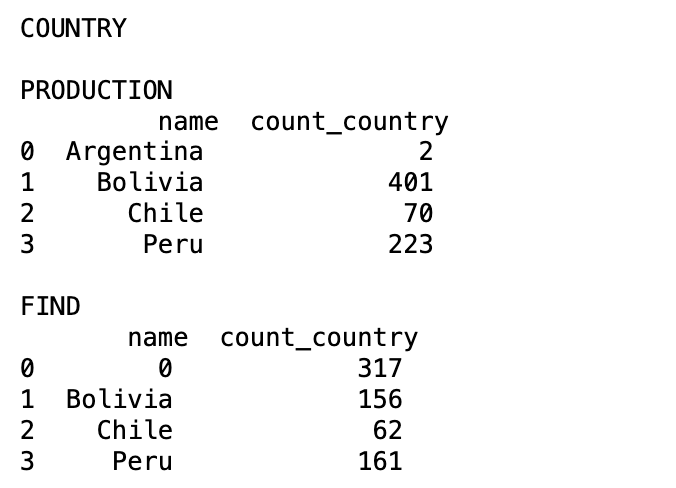
\includegraphics[width=0.4\textwidth]{../images/count_country.png}
    \caption{Nombre de textiles disponibles par pays.}
    \label{fig:tab_count}
\end{wrapfigure}

Pour obtenir la répartition géographique des pièces textiles de la base de données dans la zone andine, nous pouvons commencer par regarder leur répartition avec différents niveaux de granularité.

Dans le cas des pays, les statistiques nous renseignent sur les choix réalisés au sein de la base de données. Le Pérou détient plus de textiles découverts, conséquence de la meilleure conservation des textiles sur la côte. Dans le cas des lieux de production, la concentration bolivienne s'explique par la répartition des musées dont les collections composent la base de données. En effet, les collections ethnographiques de la base de données sont principalement issues de musées boliviens. Cette répartition est donc à la fois une conséquence de la constitution de la base de données et une conséquence de la réalité textile. Toutefois, observer la répartition par pays nous fournit peu d'informations sur les textiles dans la zone andine. C'est pourquoi affiner la granularité au niveau régional nous permettra de mieux saisir cette répartition.

\clearpage

\begin{figure}[!h]
    \begin{minipage}[c]{.5\linewidth}
            \begin{center}
                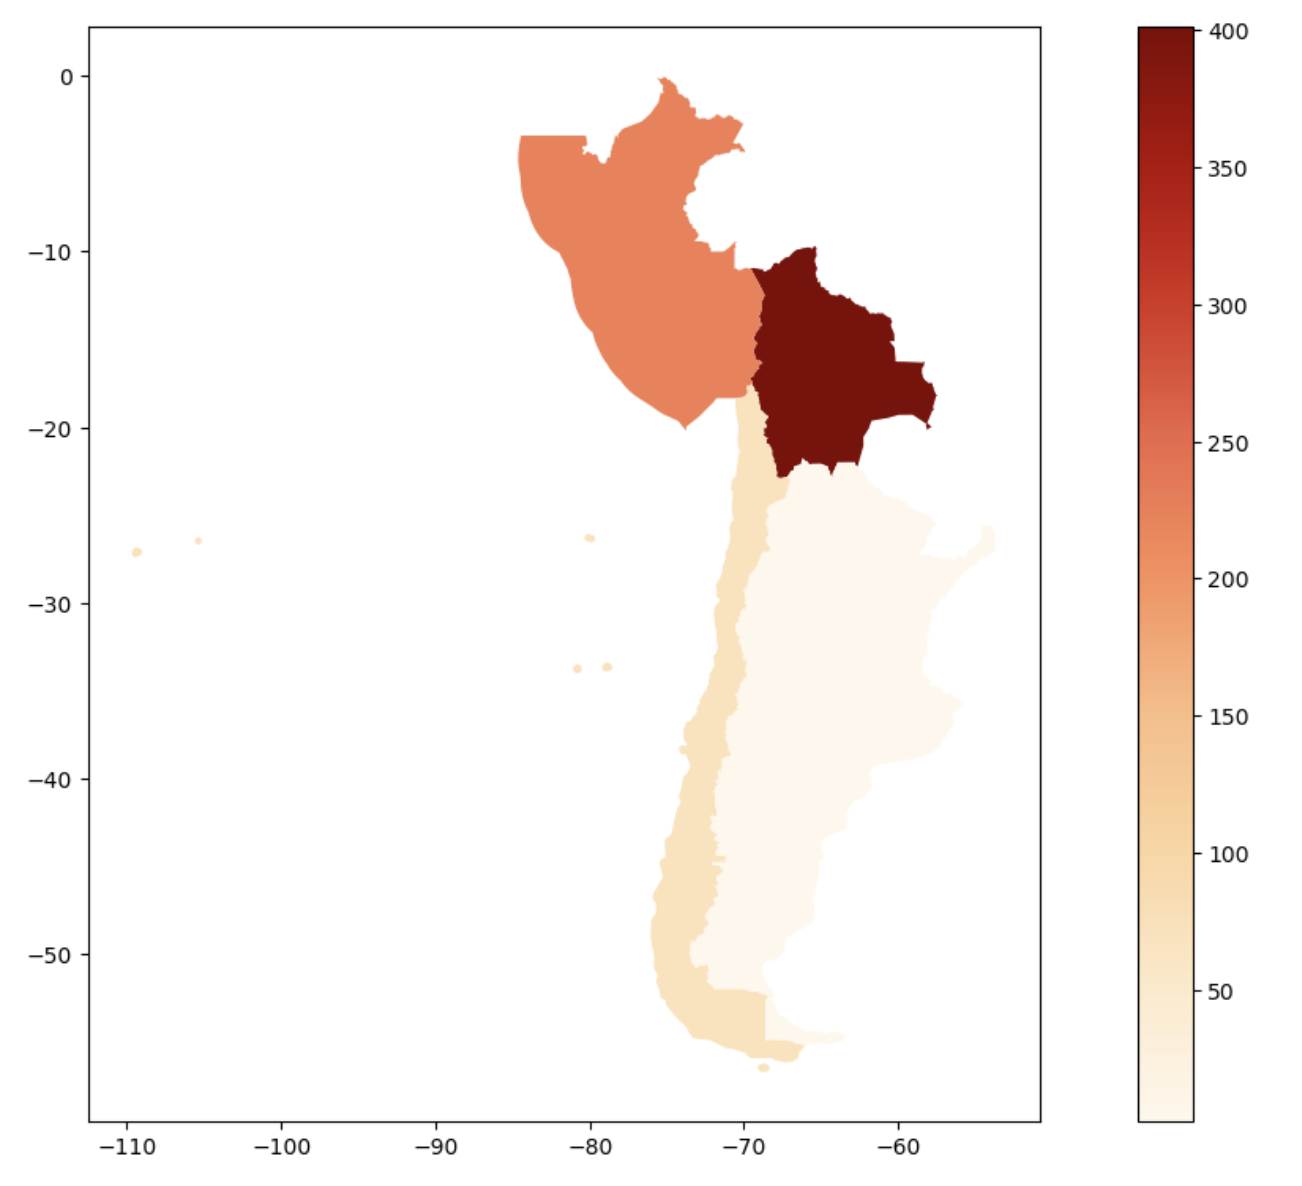
\includegraphics[height=8cm]{../images/map_count_prod.png}
            \end{center}
    \end{minipage}
        \begin{minipage}[c]{.5\linewidth}
        \begin{center}
        		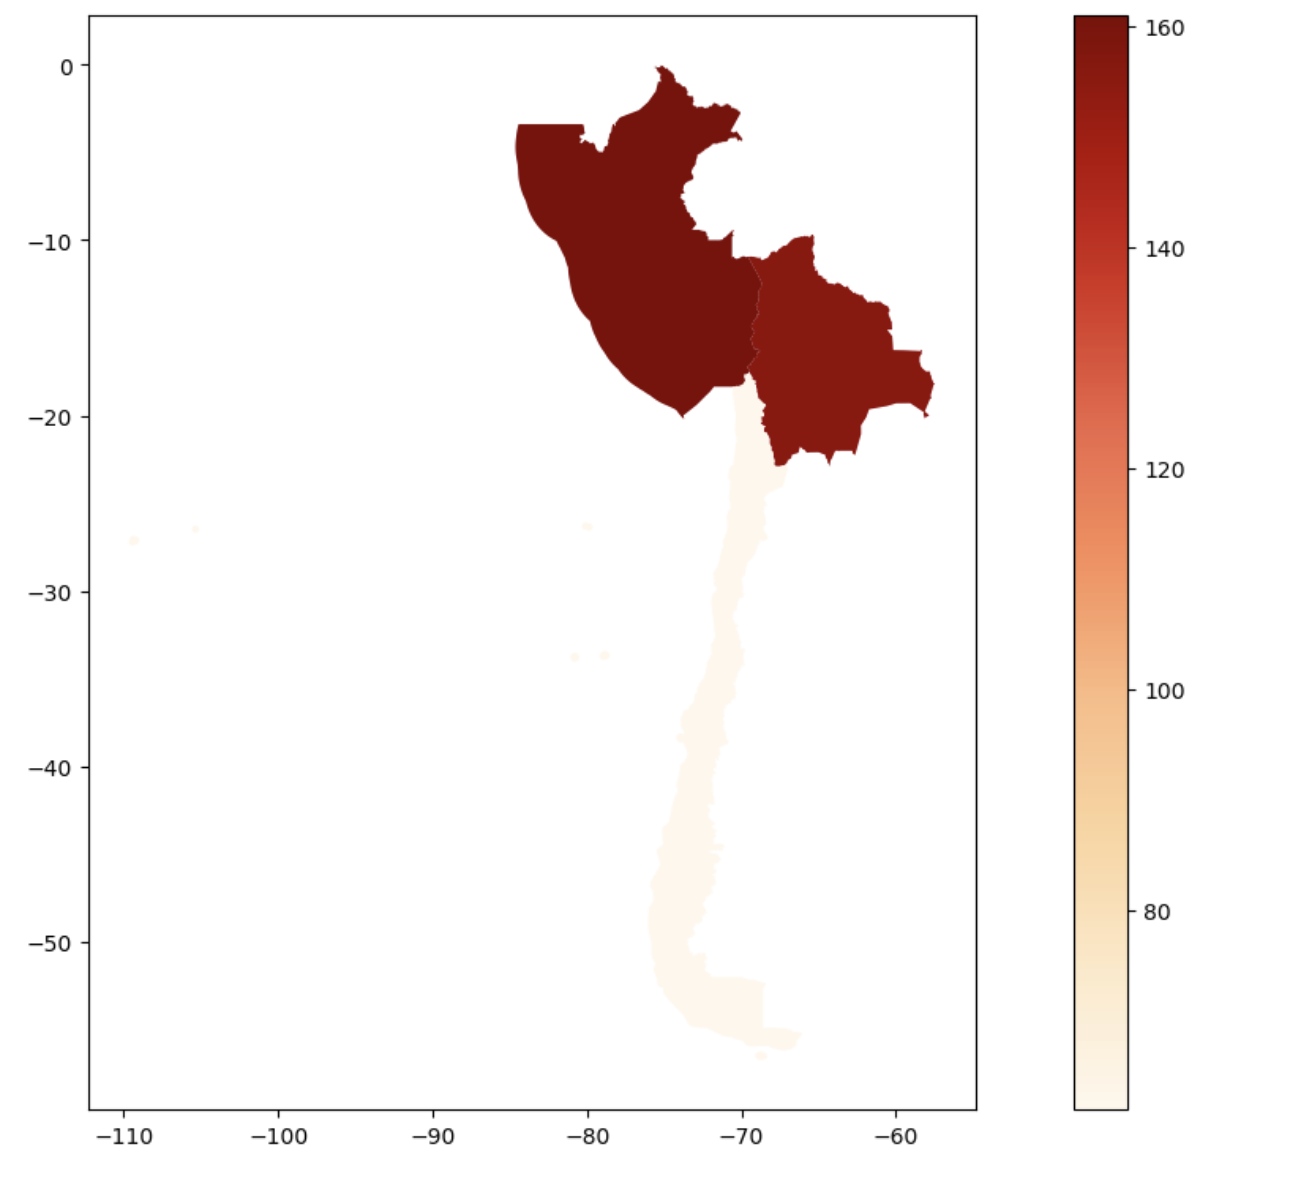
\includegraphics[height=8cm]{../images/map_count_find.png}
	\end{center}
    \end{minipage}
    \caption{Nombre de textiles par pays pour les lieux de productions et pour les lieux de découvertes.}
    \label{fig:geo_count_country}   
\end{figure}

La répartition au niveau régional nous donne des indications similaires mais de manière plus fine. La concentration des textiles produits dans l'Altiplano nord (229 pièces sur 696) nous fournit une information sur la construction de la base de données. L'ILCA a fourni au projet un ensemble de 158 maquettes textiles contemporaines, reproduites dans l'Altiplano nord à partir de motifs locaux imités (voir page \pageref{fig:maquette}). En retirant ces 158 maquettes, nous obtenons une répartition des textiles produits relativement équilibrée dans les hautes-terres.

Les régions de découvertes des textiles sont concentrées dans deux régions, la côte centrale péruvienne et l'Altiplano central. Dans le cas de la côte centrale, il s'agit uniquement de textiles archéologiques, principalement de l'Intermédiaire Récent. Dans le cas de l'Altiplano central, 70\% des textiles \og découverts \fg \:dans la zone sont des textiles ethnographiques.

\begin{figure}[!h]
    \begin{minipage}[c]{.5\linewidth}
            \begin{center}
                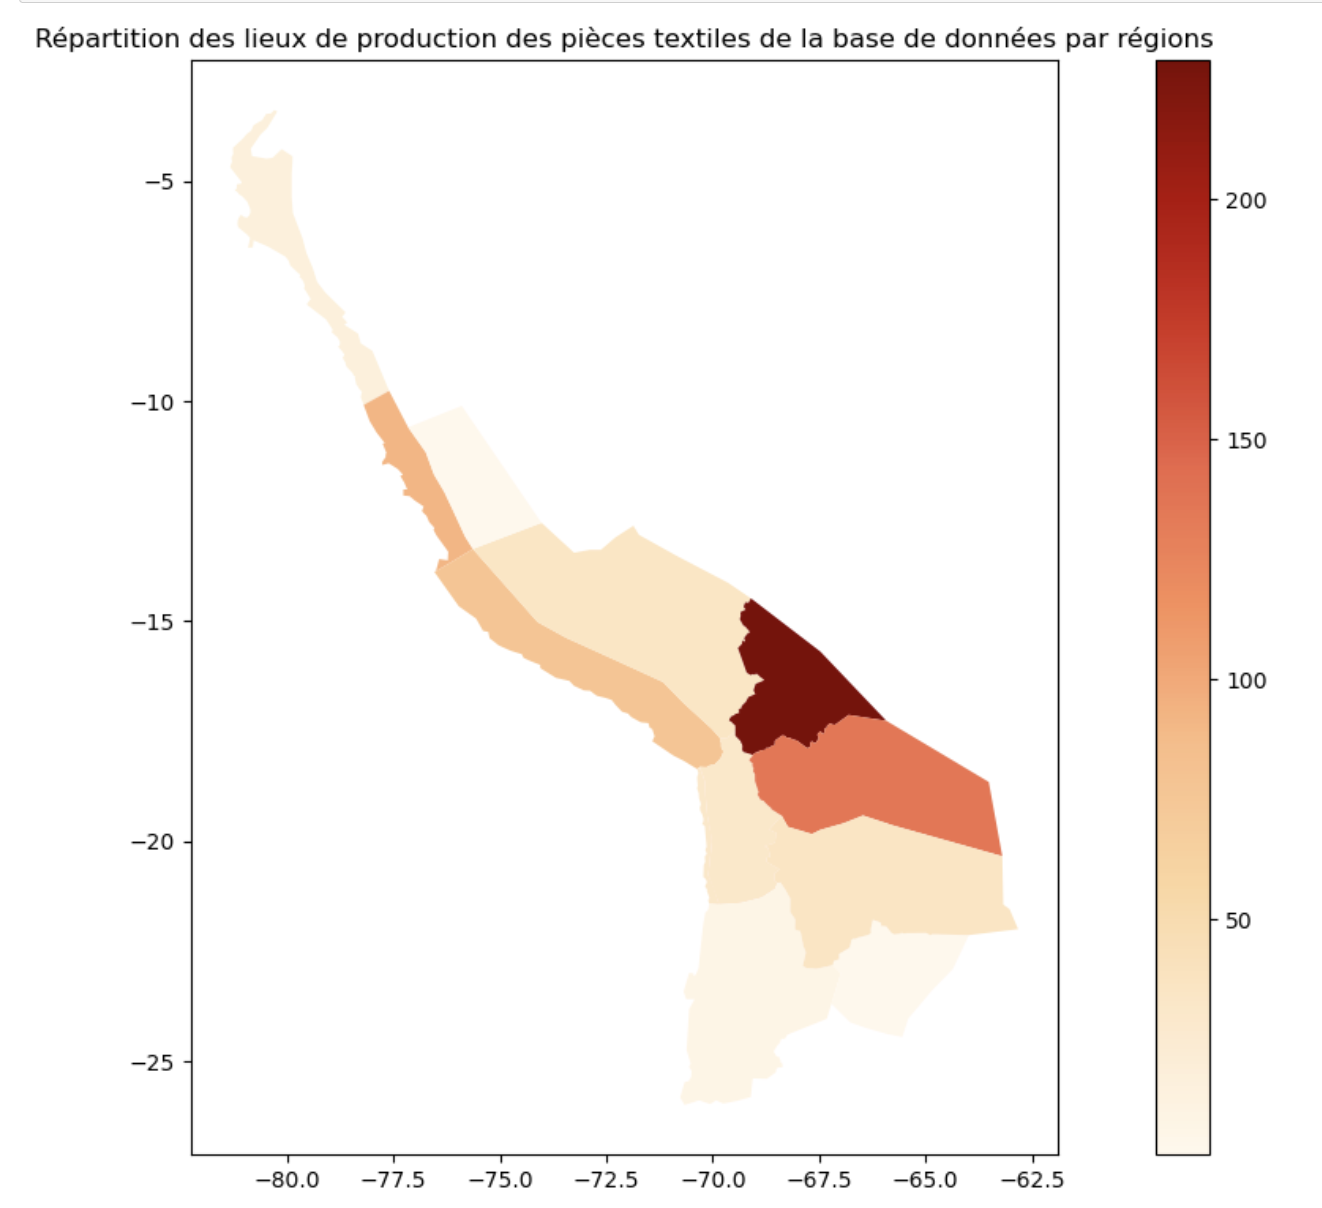
\includegraphics[height=7cm]{../images/geo_region_prod.png}
            \end{center}
    \end{minipage}
        \begin{minipage}[c]{.5\linewidth}
        \begin{center}
        		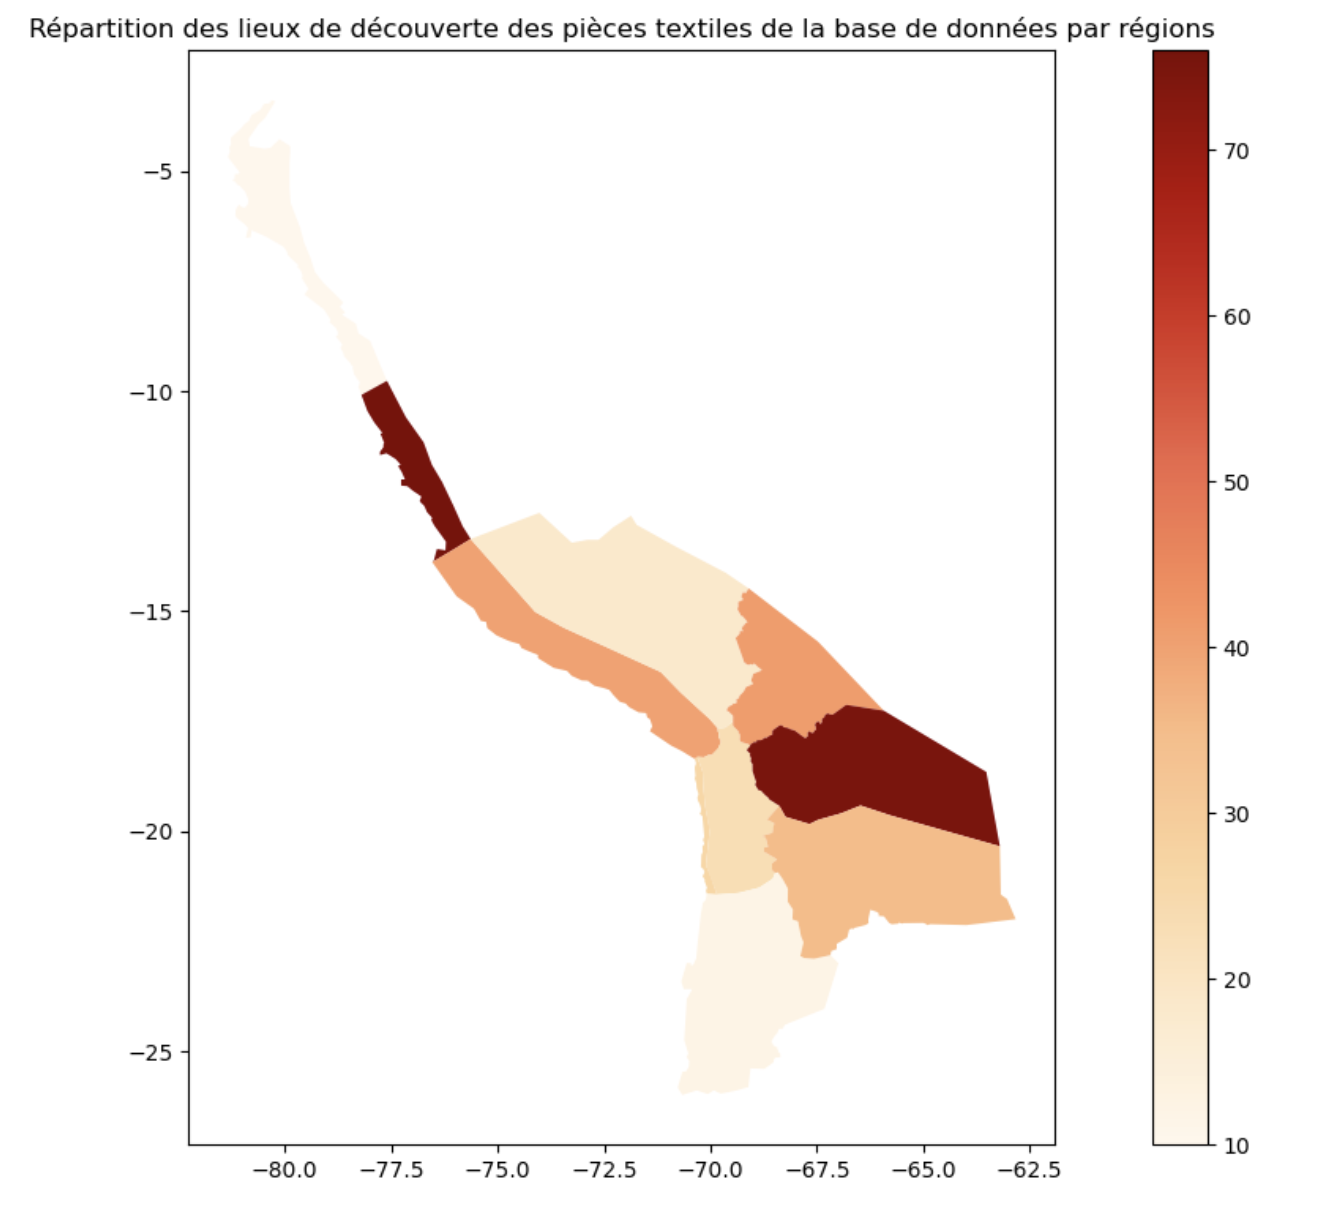
\includegraphics[height=7cm]{../images/geo_region_find.png}
	\end{center}
    \end{minipage}
    \caption{Répartition par région textiles du nombre de textiles pour les lieux de productions et pour les lieux de découvertes.}
    \label{fig:geo_count_region}   
\end{figure}

\clearpage

\begin{figure}[!h]
    \begin{minipage}[c]{.5\linewidth}
            \begin{center}
                \includegraphics[height=8cm]{../images/count_region.png}
            \end{center}
            \caption{Nombre de textiles disponibles par régions.}
            \label{fig:tab_region_count}   
    \end{minipage}
\hspace{5pt}
        \begin{minipage}[c]{.5\linewidth}
        \begin{center}
        		\includegraphics[height=8cm]{../images/MEE008A_IMG_7128.jpg}
	\end{center}
	\caption{Maquette réalisée par des tisserandes de l'Altiplano nord et données à l'ILCA. \\ Référence dans la base de données : MEE008A}
	\label{fig:maquette}   
    \end{minipage}
\end{figure}

Dans une logique exploratoire et de présentation des données, nous pouvons réaliser des cartes interactives en utilisant les localisations précises des textiles récupérées par le géocodage. Pour cela, nous avons utilisé la librairie Folium qui permet de réaliser des cartes avec Leaflet, un outil de cartographie en langage JavaScript. L'option \og cluster \fg \: dans la carte permet une meilleure visibilité en regroupant les points les plus proches. En zoomant, il est possible de voir la localisation précise et en cliquant sur le point, l'utilisateur peut obtenir l'image du textile, son identifiant dans la base de données, ainsi que son lieu de production ou de découverte selon la carte.
Pour pouvoir afficher les images, nous avons eu recours à un script de redimensionnement qui réduit le plus petit côté de l'image à 100 pixels et le plus grand proportionnellement à cette réduction\footnote{Les cartes interactives sont accessibles aux liens suivants: \url{https://lisebernard.github.io/carte_find_clustering.html} et \url{https://lisebernard.github.io/carte_prod_clustering.html}. Le script de redimensionnement des images est nommé rescale\_images.ipynb.}.

\begin{figure}[!h]
	\begin{center}
		\includegraphics[width=12cm]{../images/carte_leaflet2.png}
		\caption{Détail de la carte interactive avec affichage d'une photographie du textile ainsi que de son identifiant et son lieu de production.}
		\label{fig:leaflet}
	 \end{center}
\end{figure}

\clearpage


\section{Répartition et mobilités des textiles de la base de données}

\subsection{Mettre en évidence les foyers textiles grâce aux cartes de densité}

Pour essayer de détecter les foyers les plus denses en productions et en découvertes textiles, nous pouvons avoir recours à des cartes de densité\footnote{Les cartes de densité ont été réalisées en Python avec la librairie Matplotlib. Leur code est disponible dans le script traitement\_maps.ipynb.}. Ces cartes permettent de visualiser les zones comportant le plus d'entités ponctuelles (de points) sur la carte. Elles illustrent la répartition des données. Pour cela, nous appliquons aux points une estimation par noyau (ou \textit{kernel density estimation}) qui estime la densité de probabilité d'une variable aléatoire non-paramétrique. Dans notre cas, il faut retirer la variable \og Rapa Nui \fg \:dont la prégnance déséquilibre le calcul. Pour avoir le détail de la densité des points, nous pouvons également réaliser des cartes interactives avec Leaflet qui prennent en compte le nombre de textiles associés à un point. Contrairement aux cartes précédentes, elle permettent de récupérer à la fois la répartition globale et l'information ponctuelle de densité\footnote{Les cartes interactives sont accessibles aux liens suivants : \url{https://lisebernard.github.io/heatmap_prod.html} et \url{https://lisebernard.github.io/heatmap_find.html}}. Les cartes interactives sont certes un outil exploratoire mais elles viennent également compléter les cartes fixes puisqu'elles permettent d'obtenir le lieux précis et le nombre de textile pour chaque point.

\begin{figure}[!h]
    \begin{minipage}[c]{.5\linewidth}
            \begin{center}
                \includegraphics[height=8cm]{../images/densitymapprod.png}
            \end{center}
            \caption{Carte de densité des lieux de production des textiles.}
            \label{fig:densityProd}   
    \end{minipage}
\hspace{5pt}
        \begin{minipage}[c]{.5\linewidth}
        \begin{center}
        		\includegraphics[height=8cm]{../images/densitymapfind.png}
	\end{center}
	\caption{Carte de densité des lieux de découverte des textiles.}
	\label{fig:densityFind}   
    \end{minipage}
\end{figure}

 \begin{figure}[!h]
	\begin{center}
		\includegraphics[width=12cm]{../images/heatmap_leaflet.png}
		\caption{Détail de la carte de densité des lieux de production interactive avec affichage du lieu et du nombre de textiles provenant du lieu.}
		\label{fig:leaflet_density}
	 \end{center}
\end{figure}

Dans le cas des lieux de production, un des foyers centraux se trouve dans la région de La Paz (capitale bolivienne). Dans les Andes, les points sont concentrés sur la cordillère Est de l'Altiplano et au niveau du lac Titicaca. Les quelques points épars au nord des hautes-terres sont situés dans la région de Cuzco. Sur la côte, les points sont éparpillés avec un foyer un peu plus important sur la côte centrale au niveau de Lima. 

Dans le cas des lieux de découverte, les foyers en altitude sont plus au sud que pour les lieux de production. Ils se situent plutôt dans la région de Potosí. Sur la côte, la zone d'Arica au sud se distingue largement avec deux foyers archéologiques importants. Au niveau de la côte centrale, la zone de Lima est également dense avec plusieurs foyers archéologiques. Au sud de Lima, on trouve les deux foyers textiles les plus connus et étudiés : Nazca et Paracas.

Pour mieux comprendre la répartition de ces foyers, nous pouvons développer une approche diachronique en produisant des cartes de densité par période étudiée\footnote{Le calcul de densité est calculé indépendamment pour chaque période, les couleurs sur chaque carte ne sont donc pas équivalentes en quantité de textile mais indiquent plutôt une valeur relative de densité d'un lieu par rapport à un autre sur la période étudiée.}. 

Les époques de la période Initiale et de l'Horizon Ancien n'ont qu'un seul point géolocalisé ce qui ne permet pas de réaliser un calcul de densité. Nous pouvons tout de même observer l'origine de ces textiles, l'un sur la côte sud, l'autre au niveau de Lima, sur la côte centrale.

\begin{figure}[!h]
	\begin{center}
		\includegraphics[width=15cm]{../images/carteEH.png}
		\caption{Position des points pour la période Initiale et l'Horizon Ancien.}
		\label{fig:carteEH}
	 \end{center}
\end{figure}

\begin{figure}[!h]
	\begin{center}
		\includegraphics[width=13cm]{../images/diachDensityProd.png}
		\caption{Carte de densité diachronique des lieux de productions des textiles.}
		\label{fig:density_prod}
	 \end{center}
\end{figure}

\noindent Les textiles de la période Intermédiaire Ancienne sont également produits sur la côte, avec deux foyers importants à cette période : Nazca et Paracas\footcite[p.~58-59]{boissiereAtlasAmeriquePrecolombienne2022}.
À partir de l'Horizon Moyen, période marquée par la diffusion des civilisations Huari et Tiwanaku\footnote{Ibid., p.~68-69}, des fragments de textiles sont disponibles sur tout le territoire andin. Les foyers Nazca et Paracas persistent avec un phénomène de métissage entre les styles côtiers et l'influence de l'empire Huari provenant des Andes centrales. L'exemple présenté ici (photographie \ref{fig:VAM012}) montre la persistance du motif de serpents entremêlés relevé dès l'Horizon Ancien\footcite[p.~1]{desrosiersRevisitingOcucajeOpened2008}.

\noindent Tout au sud, le foyer textile dans le désert d'Atacama et à Arica illustre les phénomènes d'échanges à cette période. Les textiles de cette zone sont principalement composés en styles locaux (Cabuza, Maytas-Chiribaya, Coyo ou Quitor) mais des textiles se distinguent par l'influence de la culture Tiwanaku (voir photographie \ref{fig:SPA012}). L'influence Tiwanaku s'observe également dans les hautes-terres boliviennes, à Puqui, avec des textiles de style local mais également un textile qui reprend des éléments iconographiques Tiwanaku, notamment les bordures composées de fils colorés (pour un exemple de textile Tiwanaku, découvert dans les hautes-terres voir page \pageref{fig:MNA037}). Pour le reste des hautes-terres, le foyer principal est le foyer Mojocoya, au sein duquel les textiles sont produits et découverts sur place.

À la période Intermédiaire Récente, les foyers principaux se situent encore sur la côte. Tout au nord, un foyer est composé de textiles Chimú, provenant de la capitale de l'empire éponyme, Chan Chan. À la même période, dans les hautes-terres, c'est la culture Qaraqara qui compose un foyer. Il s'agit d'une \og confédération d'ethnies régionales et de seigneuries préhispaniques \fg \:organisées après la chute de l'empire Tiwanaku\footnote{\cite[p.~309]{oriasReviewQaraqaraCharkaMallku2009}. Citation originale : \textquotedblleft \textit{confederación de etnias regionales y señoríos prehispánicos}\textquotedblright}. Ces textiles sont relativement simples, en terme de techniques et de motifs, puisqu'avec la partition régionale typique des périodes intermédiaires, les styles iconographiques se simplifient\footcite[p.~288]{coveyMultiregionalPerspectivesArchaeology2008}.
\begin{figure}[!h]
    \begin{minipage}[c]{.5\linewidth}
    \begin{center}
     	\includegraphics[width=6cm]{../images/VAM012.jpg}
     	\caption{Tunique dans un style qui mélange éléments Nazca et Huari. \\ Référence dans la base de données : VAM012}
    	\label{fig:VAM012}
    \end{center}
    \end{minipage}
    \hspace{5pt}
    \begin{minipage}[c]{.5\linewidth}
        		\begin{center}
         		\includegraphics[width=6cm]{../images/SPA012.jpg}
         		\caption{Éléments iconographiques Tiwanaku sur une tunique provenant de la région d'Atacama. \\ Référence dans la base de données : SPA012}
			\label{fig:SPA012}
		\end{center}
	\end{minipage}
\end{figure}

\begin{wrapfigure}{r}{0.4\textwidth}
	\begin{center}
		\includegraphics[width=3cm, angle=-90]{../images/MCM014.jpg}
		\caption{Exemple de textile Qaraqara.\\ Référence dans la base de données : MCM014}
		\label{fig:MCM014}
	 \end{center}
\end{wrapfigure}

Au cours de l'Horizon Récent, marqué par le développement de l'empire Inca, les foyers précédents persistent, notamment les Chimú dont la chute arrive en 1470, date du début de l'Horizon Récent dans la base de données. Les textiles de cette période dans la base de données sont tous catégorisés comme Incas. 

Les textiles coloniaux et républicains proviennent exclusivement des hautes-terres du sud du Pérou et de l'Altiplano bolivien. À partir de ces périodes, il est plus compliqué de penser les textiles en termes de foyers de production. Comme déjà mentionné, les espagnols participent amplement à la diffusion des styles entres populations. Les foyers apparaissant sur les cartes sont alors plutôt des indicateurs des collections muséales composant la base de données. Toutefois, elles illustrent bien la disparition progressive des pratiques de tissage sur la côte avec la progression des hautes-terres dans la domination de la pratique textile andine. \clearpage

%Huari : BML106 / MSF041 / MNA014 / MSF051 / MSF060 --> dans la sierra MSF018
%Tiwanaku : BML012 / BML013 / BML013 / MCM025 (pour la côte sud) --> pour Atacama et Arica : SPA003 (provincial) / MMA082-87/MMA087/MMA089-91/MMA093-97/MSF016/MSF029/SPA003/SPA012
%BML087 Chancay pendant Middle Horizon ? 
%Autre cas Tiwanaku dans les hautes-terres : MNA035 / MNA037 /SPA001 / SPA009

\begin{figure}[!h]
	\begin{center}
		\includegraphics[width=15cm]{../images/diachDensityFind.png}
		\caption{Carte de densité diachronique des lieux de découvertes des textiles.}
		\label{fig:density_find}
	 \end{center}
\end{figure}

Pour les lieux de découverte, les foyers apparaissant sur les cartes de densité sont similaires puisqu'il s'agit principalement des mêmes textiles dont les lieux de production et de découverte se situent au même endroit. Disposant de moins de données pour les lieux de découverte, la répartition de la densité est moins dispersée ce qui donne une densité plus lissée avec moins d'extrêmes. En comparaison avec les lieux de production, à la période Intermédiaire Ancienne, les textiles Paracas sont moins denses que les textiles Nazca. Il en est de même à l'Horizon Moyen, au cours duquel on retrouve les mêmes foyers principaux mais moins de foyers secondaires. Á la période Intermédiaire Récente, les textiles sont concentrés sur la côte avec moins de foyers Qaraqara dans les hautes-terres et plus de concentration à Arica, notamment avec les excavations de la Playa Miller de style Pocoma. Au niveau des côtes centrale et sud, les civilisations côtières dominent avec notamment des textiles Chimú, Ichma et Chancay. À l'Horizon Récent, seuls trois foyers apparaissent le long de la côte avec la persistance d'Arica au sud, Nazca au milieu et Lima au nord. Aux périodes coloniale et républicaine, les foyers de découverte sont moins épars et plus concentrés sur l'Altiplano central. 

\subsection{Saisir les mobilités par des calculs de distances}

Cartographier les textiles nous a permis de saisir leur répartition et leur densité sur le territoire andin. En outre, dans le cas où les textiles disposent d'un lieu de production et d'un lieu de découverte distincts, nous pouvons saisir les circulations physiques des textiles. Ne détenant que deux localisations, un point de départ et un point d'arrivée, nous ne sommes pas en mesure de saisir les parcours des textiles mais nous pouvons saisir certaines circulations avec des distances à vol d'oiseau\footnote{Les calcul de distance et leur cartographique sont disponibles dans le script traitement\_maps.ipynb.}.

\begin{figure}[!h]
	\begin{center}
		\includegraphics[width=16cm]{../images/tabDistance.png}
		\caption{Tableau des cas de textiles dont le lieu de découverte est à plus de 5 kilomètres \\ de son lieu de production. Les couleurs indiquent des mobilités géographiquement similaires.}
		\label{fig:distancetab}
	 \end{center}
\end{figure}

\clearpage

\begin{wrapfigure}{l}{0.2\textwidth}
    \centering
    \includegraphics[width=0.2\textwidth]{../images/stat_distance.png}
    \label{fig:distance}
\end{wrapfigure}

\noindent Sur les 696 textiles référencés dans la base de données, 74 ont un lieu de découverte distinct de leur lieu de production. La distance moyenne séparant le lieu de découverte et le lieu de production dans le cas où ils sont distincts est de 121,70 kilomètres, la plus petite étant de 350 mètres et la plus grande de 1497,44 kilomètres. Toutefois, la médiane est à 1,51 kilomètre. Les distances sont donc plutôt réduites et les plus petites distances sont probablement liées à la géolocalisation. Par exemple, les textiles découverts à \textit{Playa Miller} ont été produits à Arica soit à 1 kilomètre de leur lieu d'excavation. Il en est de même pour les textiles provenant des fosses d'Azapa qui ont été produites à San Miguel de Azapa, à 1,5 kilomètres de là. Ces cas dont le lieu de découverte est situé à moins de 5 kilomètres du lieu de production sont au nombre de 42, nous avons décidé de les supprimer de la représentation graphique pour ne pas surcharger la carte et pour se concentrer sur les textiles qui ont plus amplement circulé. Nous obtenons alors une liste de 32 textiles dont les lieux de découverte sont à plus de 5 kilomètres de leurs lieux de production.

\noindent Dans notre base de données, ces mobilités apparaissent à partir de l'Horizon Moyen (600 avant J.C.) et s'étendent jusqu'à la période républicaine. Les mobilités semblent plus intenses au cours de l'Horizon Moyen et de la période Intermédiaire Récente. 
L'Horizon Récent ne présente qu'un seul cas de mobilité physique avec un textile produit à Pachacamac et découvert à Lima (en gris dans le tableau \ref{fig:distancetab}). Pachacamac était un centre administratif et religieux central de la période Intermédiaire Ancienne à l'empire Inca, et son influence portait sur la région de Lima. Il n'est donc pas surprenant que ce textile se trouve ainsi à 25 kilomètres de son lieu de production. 

Au cours de l'Horizon Moyen, plusieurs textiles voyagent depuis les hautes-terres boliviennes vers le bassin de l'Atacama au nord du Chili (en rouge dans le tableau \ref{fig:distancetab}), soit plus de 600 kilomètres de distance. Ces trois textiles sont de style Tiwanaku et confortent l'hypothèse d'une influence de l'empire Tiwanaku sur le sud de la zone andine que nous avons déjà souligné avec l'exemple \ref{fig:MNA037}. Le travail d'Alex Nielsen sur la circulation d'objets atteste des routes commerciales entre ces deux zones\footnote{\cite[p.~407]{nielsenCirculatingObjectsConstitution2013}, voir figure 16.16}. En outre, les tuniques locales d'Atacama imitent des textiles Tiwanaku, probablement à partir des modèles qui sont arrivés depuis les hautes-terres boliviennes. La comparaison de ces exemples est d'autant plus intéressante qu'elle semble illustrer le phénomène d'imitation dont nous parlions dans le premier chapitre du mémoire. En effet, les manches du textile SPA012 (photographie \ref{fig:SPA012}) de style Tiwanaku sont réalisées en broderie. Or, dans le cas du textile qui vient des hautes-terres ce même type de motif est réalisé en tresses adjointes au tissage à dominante chaîne. % A vérifier 
Il pourrait donc s'agir d'une imitation iconographique en modifiant la technique\footnote{Cette hypothèse mériterait d'être vérifiée, d'une part en ayant accès au textile pour les caractéristiques techniques, et d'autre part en le comparant à d'autres cas similaires.}.

\begin{figure}[!h]
    \begin{minipage}[c]{.5\linewidth}
            \begin{center}
                \includegraphics[height=7cm]{../images/SPA009.jpg}
            \end{center}
            \caption{Détail d'un textile Tiwanaku produit dans les hautes-terres et découverts dans le bassin de l'Atacama (Horizon Moyen). Référence dans la base de données : SPA009.}
            \label{fig:SPA009}   
    \end{minipage}
\hspace{5pt}
        \begin{minipage}[c]{.5\linewidth}
        \begin{center}
        		\includegraphics[height=7cm]{../images/BML035.jpg}
	\end{center}
	\caption{Sac produit à Azapa et découvert à Trujillo (Horizon Moyen). \\ Référence dans la base de données : BML035}
	\label{fig:BML035}
    \end{minipage}
\end{figure}

\noindent À la même période, sur la côte sud du Pérou des textiles circulent entre Ica, Nazca et Paracas (en bleu dans le tableau \ref{fig:distancetab}). Ces trois zones sont très proches et il n'est pas surprenant que les textiles des civilisations locales s'échangent dans cette zone. D'autant plus que les deux textiles référencés sont de style Nazca-Huari (photographie \ref{fig:VAM012}), s'inscrivant donc dans l'aire d'influence commune de l'empire Huari.
Enfin, un textile sort du lot (en rose dans le tableau \ref{fig:distancetab}), il s'agit d'un sac cérémoniel destiné à la coca, dans un style local d'Azapa (côte nord du Chili) découvert à Trujillo (nord du Chili), soit à 1497,44 kilomètres de son lieu de production. Ce textile est très mystérieux et je ne suis pas en mesure d'expliquer le trajet qu'il a pu effectuer entre son point de départ et son point d'arrivée. Son rôle religieux pourrait expliquer sa circulation. Il confirme la réalité des échanges textiles sur la longue distance dans la zone andine.

\begin{wrapfigure}{r}{0.6\textwidth}
    \centering
    \includegraphics[width=0.6\textwidth]{../images/BML014.jpg}
    \caption{Fragment Chancay retrouvé à Cuzco. \\ Référence dans la base de données : BML014}
    \label{fig:BML014}
\end{wrapfigure}

À la période Intermédiaire Récente, deux types de mobilités apparaissent. Les textiles qui circulent au sein de la côte centrale (en jaune dans le tableau \ref{fig:distancetab}) et les textiles qui circulent entre la côte centrale et la côte nord (en vert dans le tableau \ref{fig:distancetab}). Dans le premier cas, il s'agit de textiles dont la mobilité fait moins de 100 kilomètres. Ce sont des tissus Chancay retrouvés à Lima, soit dans la zone d'influence de cette civilisation\footcite[p.~72]{boissiereAtlasAmeriquePrecolombienne2022}.
 Il en est de même pour les textiles Chimú de la côte nord du Pérou, qui sont originaires de la capitale Chan Chan et découverts à Lima, soit près de 500 kilomètres plus au sud mais dans l'aire d'influence de cette civilisation.
Un cas se distingue à cette période, le fragment BML014, textile Chancay retrouvé à Cuzco. De la même manière, son parcours et ses conditions de conservation ne sont pas spécifiées mais il pourrait être l'indice d'une circulation des textiles sur de longues distances à cette période.

Les derniers cas (en blanc dans le tableau \ref{fig:distancetab}) sont les textiles post-coloniaux. Ils composent la quasi-totalité des mobilités inter-andines des hautes-terres boliviennes (voir carte \ref{fig:distance_map}). Là non plus, nous n'avons pas leur parcours et nous ne pouvons donc que proposer des hypothèses quant à leur circulation. À partir de la période coloniale, les relations marchandes se développent de manière croissante dans les Andes, notamment les échanges commerciaux de textiles. Ces échanges marchands sont la première hypothèse de circulation des textiles dans cette zone, notamment pour les textiles retrouvés à La Paz, capitale bolivienne au c\oe{}ur des échanges économiques du pays.

Nous pouvons observer sur la carte suivante, pour les 32 cas étudiés, les lieux de production, les lieux de découverte et la distance à vol d'oiseau qui les sépare (en vert). Grâce au paramètre \textit{alpha} des couleurs dans la librairie Python Matplotlib nous avons pu ajouter de la transparence pour garder une information de densité. Ainsi, les points les plus intenses indiquent une multitude de textiles et les points violets indiquent qu'un lieu est à la fois origine et destination des textiles.

\begin{figure}[!h]
	\begin{center}
		\includegraphics[width=15cm]{../images/carteDistance.png}
		\caption{Carte reprenant les distances entre les lieux de production (en rouge) et les lieux de découverte (en bleu) des textiles.}
		\label{fig:distance_map}
	 \end{center}
\end{figure}

Après un large travail d'homogénéisation des données en ligne avec l'état de l'art, nous avons pu proposer une première analyse géographique diachronique des textiles du corpus. Ces cartographies confirment la répartition des textiles sur le territoire andin tel qu'expliqué par les conditions de conservation et par le développement des civilisations sur le territoire. En outre, le géocodage des lieux de production et de découverte des textiles nous ont permis de mettre au jour des mobilités plus ou moins intenses entre civilisations pré-hispaniques. Néanmoins, l'analyse des métadonnées des textiles ne nous permet pas de saisir les évolutions iconographiques des textiles. C'est pourquoi dans le dernier temps du mémoire, nous allons nous appuyer sur le corpus de photographies de la base de données \textit{Weaving Communities of Practice} afin de tester nos hypothèses d'imitations techniques et iconographiques.
\chapter{Mobiliser des outils de \textit{computer vision} pour relever les imitations et ré-interprétations techniques et iconographiques}
\markboth{}{}

\epigraph{\og In Andean textiles, there is a deep harmony between image and structure.\fg}{William J. Conklin, 1997, \og Structure as Meaning in Andean Textiles. \fg, p.~118.}


\section{Analyse des sources iconographiques}
\subsection{Les images : sources de savoir sur les influences iconographiques ?}

Les données géographiques de la base de données nous ont permis de détecter certains foyers de production textile ainsi que certaines circulations physiques des pièces.  Des circulations textiles ont certes lieu mais, comme nous l'avons vu dans le premier chapitre du mémoire, une partie des évolutions des tissus se fait par imitations ou ré-interprétations iconographiques et techniques. Ces modifications sont détectables en analysant directement les objets et le recours à des outils de \textit{computer vision} semblent adéquats pour les saisir. Nous entendons par \textit{computer vision}, le domaine de l'intelligence artificielle qui, à partir d'images numériques, obtient des informations significatives sur celles-ci.

Certaines sociétés se sont influencées à travers les conquêtes mais aussi par les échanges ou la proximité géographique. 
Ainsi, les sociétés voisines Chimú et Chancay, sur la côte centrale du Pérou, partagent des traits culturels communs. Dans la base de données, nous pouvons observer cela à partir de poupées utilisées dans les sépultures. Elles représentent la même divinité homme-ours. Leurs visages sont réalisés en tricot dont partent des cordons et une frange qui forment le corps et les cheveux. Les traits du visage sont formés par quelques points simples de broderie (passé-plat ou chaînette). Ce cas nous montre la complexité de la compréhension des influences entre civilisations, puisqu'il s'agit de civilisations voisines en conflit mais qui ont probablement eu des échanges et dont on sait qu'elles partageaient certaines pratiques rituelles et croyances. Saisir les influences permet donc d'aller au-delà des changements iconographiques et techniques et de saisir l'évolution de traits culturels fondamentaux dans les sociétés, comme les pratiques rituelles d'inhumation. 


\begin{figure}[!h]
    \begin{minipage}[c]{.5\linewidth}
            \begin{center}
                \includegraphics[width=5cm]{../images/BML059.jpg}
            \end{center}
    \end{minipage}
        \begin{minipage}[c]{.5\linewidth}
        \begin{center}
        		\includegraphics[width=5cm]{../images/VAM018.jpg}
	\end{center}
    \end{minipage}
   \caption{Poupées d'enterrement Chancay et Chimú tardif. \\ Références dans la base de données : BML059 et VAM018.}
   \label{fig:poupees}
\end{figure}


Comme nous l'avons vu, à l'Horizon Récent, les cultures s'influencent avec la culture Inca qui s'impose sur tout le territoire tout en gardant les spécificités locales des populations\footcite[p.~53]{nilesArtistEmpireInca1994}.
Le textile ci-dessous mélange ainsi le style inca, par les couleurs, la forme du sac, la technique à dominante chaîne et les finitions des bordures, avec le style Chimú sur la lanière en double-étoffe qui contient des personnages anthropomorphiques typiques de cette civilisation.
\begin{figure}[!h]
	\begin{center}
		\includegraphics[width=10cm]{../images/MSF066.jpg}
		\caption{Exemple de textile métissé entre Chimú et Inca. \\ Référence dans la base de données : MSF066}
		\label{fig:MSF066}
	 \end{center}
\end{figure}

Ces deux cas nous amènent à réfléchir selon deux axes. Comme le soulignent Sven Helmer et Vuong M. Ngo dans leur proposition de mesure de similarité entre les textiles, comprendre la structure interne des textiles \og peut aider les experts du domaine à mieux comprendre comment les textiles ont évolué au fil du temps et se sont diffusés dans différentes régions\footnote{\cite[p.~163]{helmerSimilarityMeasureWeaving2018}. Citation originale : \textquotedblleft \textit{can help domain experts gain deeper insights into how textiles evolved over time and spread across different regions}\textquotedblright}.\fg \:Classifier les techniques à partir d'images permettrait donc de détecter si certaines sociétés partagent les mêmes traits techniques, indicateurs d'échanges ou d'influence. C'est un travail d'autant plus important qu'avec la numérisation des collections muséales les chercheurs et chercheuses travaillent de plus en plus à partir d'images d'artefacts. Par ailleurs, nous devons nous questionner sur les textiles détenant des traits iconographiques communs ou hybrides. Ce deuxième axe est d'autant plus adéquat que certains motifs sont propices à l'imitation car facilement transférables d'une technique à une autre, comme le relève Sophie Desrosiers pour les motifs \og en escalier qui peuvent être traduits en flottés de chaîne ou de trame\fg \footnote{\cite[p.~7]{desrosiersRevisitingOcucajeOpened2008} Citation originale : \textquotedblleft \textit{with stepped outlines which can be translated into warp or weft floats}\textquotedblright}. Dans les textiles andins, les motifs peuvent en effet difficilement être pensés hors des techniques puisque celles-ci contraignent la réalisation iconographique\footcite[p.~118]{conklinStructureMeaningAndean1997}. Dans le cas des textiles à dominante chaîne, l'organisation des fils, qui constitueront les motifs, doit être pensée en amont du montage sur le métier à tisser, illustrant l'imbrication entre techniques et iconographie. Ces motifs contraints sont donc possiblement détectables à partir du corpus d'images.

\subsection{Les sources iconographiques de la base de données \textit{Weaving Communities of Practice}}

La base de données \textit{Weaving Communities of Practices} est composée d'un corpus iconographique qui regroupe trois types d'images : des photographies, des croquis et des relevés textiles réalisés par logiciel de dessin assisté par ordinateur (DAO) (dans le même esprit que le relevé \ref{fig:BML044_schema}). Nous disposons de 162 modélisations par DAO, réalisées par les ingénieurs du projet. Les 83 croquis, réalisés à la main, font partie des collections du \textit{British Museum}.

\begin{figure}[!h]
    \begin{minipage}[c]{.4\linewidth}
            \begin{center}
                \includegraphics[height=6cm]{../images/BML026_IMG.jpg}
            \end{center}
    \end{minipage}
\hspace{5pt}
        \begin{minipage}[c]{.2\linewidth}
        \begin{center}
        		\includegraphics[height=6cm]{../images/BML026_Schema.png}
	\end{center}
    \end{minipage}
            \begin{minipage}[c]{.4\linewidth}
        \begin{center}
        		\includegraphics[height=6cm]{../images/BML026_croquis.jpg}
	\end{center}
    \end{minipage}
    \caption{Photographie, schéma et croquis pour un même textile. \\ Référence dans la base de données : BML026.}
\end{figure}

\noindent Le corpus d'images à partir duquel nous allons travailler ne contient ni les schémas ni les croquis, mais uniquement les photographies, soit 3301 images. Nous pouvons observer sur le schéma suivant le nombre d'images disponibles par textile et la répartition statistique de ce nombre sous forme de boîte à moustache. Les photographies sont toutes en couleur (3 canaux), elles contiennent les textiles entiers, mais également seulement une partie de celui-ci ainsi que des supports (en bois, en carton) ou des personnes les portant, notamment dans les collections du musée national archéologique de Bolivie. 

\begin{figure}[!h]
	\begin{center}
		\includegraphics[width=16cm]{../images/nbImages.png}
	 \end{center}
	 \caption{Répartition des images par objet}
\end{figure}

\begin{wrapfigure}{r}{0.3\textwidth}
    \centering
    \includegraphics[width=0.3\textwidth]{../images/IFRAO.jpg}
    \caption{Règle IFRAO}
    \label{fig:IFRAO}
\end{wrapfigure}



Une grande partie des photographies contiennent une échelle IFRAO, réglette de 10 centimètres composée de carrés noirs, blancs et colorés (vert, rouge, jaune et bleu). Parue en 1994, cette échelle permettait initialement aux archéologues de calibrer les couleurs des \oe{}uvres d'art préhistoriques\footcite[p.~225]{lopezIFRAOStandardScale2009}. Les couleurs de la règle étant fixées numériquement, elles peuvent servir de référence pour le reste de l'image et ainsi ajuster les couleurs des artefacts au sein des images numériques. La présence de cette règle nous permet d'avoir une idée précise de la taille des pièces textiles et nous confirme la disparité de ces dernières : certaines mesurent plus d'un mètre de longueur et/ou de largeur et d'autres seulement un demi centimètre. Les images ont des dimensions analogues, la plupart ont leur largeur ou leur hauteur entre 700 et 800 pixels, et l'autre côté à 1068 pixels (voir schéma suivant).

Les images de la base de données ont presque toute la même résolution (nombre de pixel contenu dans un pouce (\textit{inch}) ou pixels par pouce). La résolution des images de la base de données est plutôt faible puisqu'on considère que la résolution d'une image est bonne autour de 250~ppp. Nous n'utiliserons donc pas ce paramètre dans la suite du traitement.

\begin{table}[!h]
    \centering
    \begin{tabular}{|c|c|}
        \hline
         \cellcolor{blue!20}\textbf{Résolution (\textit{dot per inch})} & \cellcolor{blue!20}\textbf{Nombre d'images} \\ \hline \hline
         72 &  3220 \\ \hline
         96 & 2 \\ \hline
         240 & 55 \\ \hline
    \end{tabular}
    \caption{Résolution des images de la base de données.}
    \label{tab:resolution}
\end{table}

\clearpage

\begin{figure}[!h]
	\begin{center}
		\includegraphics[width=16cm]{../images/dimension.png}
	 \end{center}
	 \caption{Répartition de la dimension des images}
\end{figure}


\section{Une classification automatique des techniques ?}

\subsection{L'apprentissage machine au service de la détection des armures textiles}

Un des indicateurs des influences entre sociétés porte sur les techniques utilisées par ces civilisations. Dans la plupart des cas, les techniques sont détectables à partir des armures, c'est-à-dire de la manière dont les fils sont entremêlés. La question des techniques est centrale en analyse des textiles et l'utilisation de l'apprentissage machine pour détecter des informations techniques à partir d'images est essentielle.


Comme le soulignent  Helmer et Ngo, la variété des armures textiles complexifie leur modélisation\footcite[p.~160]{helmerSimilarityMeasureWeaving2018}. C'est d'ailleurs une des limites aux propositions contemporaines de classification des armures textiles reposant sur l'apprentissage machine. Souvent destinées à une finalité industrielle, elles s'entraînent sur des armures simples au sein desquelles la trame et la chaîne sont visibles (toile, sergé et satin)\footcite[p.~6365-6369]{mengAutomaticRecognitionWoven2022}. Pour les armures plus complexes, la détection des techniques est réalisée après un lourd processus d'annotation\footcite[p.~169]{helmerSimilarityMeasureWeaving2018}. Travailler sur les armures textiles à partir d'images pose en effet question puisqu'il s'agit de saisir une structure en trois dimensions à partir d'images en deux dimensions. Ainsi, \og le dessin d'une étoffe façonnée -- produit par le tissage -- résulte d'un entrelacement et n'est pas un dessin de surface, imprimé sur étoffe ou sur papier\fg\footcite[p.~67]{leclercqEntretienAvecJeanPaul2016}. Nous posons l'hypothèse que certains éléments apparaissant sur les faces des textiles sont discriminants pour déterminer les techniques, notamment les lisières, les directions des fils ou les zones de finition des textiles.


\begin{figure}[!h]
    \centering
    \includegraphics[width=12cm]{../images/resSimple_CardonP199.png}
    \caption[Structure simple d'un réseau de neurones]{Structure simple d'un réseau de neurones \\ Source : C\textsc{ardon} et al., 2018, p.~199}
    \label{resSimple}
\end{figure}

La classification automatique des textiles repose sur des méthodes d'apprentissage machine. Ce concept apparaît en 1943 quand Warren S. McCulloch et Walter Pitts proposent le premier modèle, dans le domaine de la neurophysiologie, qui est associé au concept d'apprentissage\footcite{mccullochLogicalCalculusIdeas1943}. C'est un modèle au sein duquel \og le neurone prend des variables en entrées, y applique un poids pour produire une somme qui, si elle dépasse un certain seuil, déclenche l'activation du neurone\footcite{cardonRevancheNeuronesInvention2018}\fg. Il faut attendre les années 2010 pour que ce type de modèle, \og réseau de neurones \fg, ainsi que ses développements dans les années 1980, soit réutilisé et adapté au traitement des images. Alex Krizhevsky, Ilya Sutskever et Geoffrey Hinton utilisent, en 2012, un réseau de neurones qui modifie profondément le domaine de la classification d'images\footcite{hintonImprovingNeuralNetworks2012}. Ils réussissent à classer un ensemble de plus d'un million d'images grâce à un réseau de neurones convolutif (CNN). Les CNN sont composés d'un ensemble de couches dont :
\begin{citer}
 	les couches additionnelles de neurones permettent d'apprendre des fonctions non linéaires. L'algorithme fonctionne en prenant la dérivée de la fonction de perte du réseau et en \textquotedblleft propage\textquotedblright \:l'erreur pour corriger les coefficients dans les couches basses du réseau\footcite[p.~198]{cardonRevancheNeuronesInvention2018}. 
 \end{citer}
 \noindent Dans notre cas, nous utiliserons le CNN \textit{You Only Look Once} (YOLO)\footcite[p.~1]{redmonYouOnlyLook2016}. Il alterne entre des couches de convolution (\textit{Conv. Layer}) au sein desquelles une fenêtre glissante parcourt l'image pour détecter les caractéristiques de l'images ou \textit{features}, et des couches de \textit{pooling} qui réduisent la taille de l'image d'entrée, en prenant la valeur maximum de la fenêtre considérée (\textit{MaxPooling})\footcite[p.~439]{lecunDeepLearning2015}. L'alternance entre ces couches permet de détecter les caractéristiques de chaque classe au niveau du détail (quand le nombre de pixels est élevé) et au niveau global (en réduisant le nombre de pixels). Ce modèle est notamment destiné à la classification d'objets, il divise l'image d'entrée en une grille de cellules, détecte les objets dans ces cellules et leur adjoint une classe. Dans notre cas, nous reprenons l'architecture de YOLO que l'on entraîne à partir de nos images et de nos classes. 
 \clearpage
 
 \begin{figure}[!h]
	\begin{center}
		\includegraphics[width=18cm]{../images/YOLO_archi.png}
		\caption{Architecture du réseau YOLO. \\ Source : Redmond \textit{et al.}, 2016, p.~3.}
		\label{fig:YOLO}
	 \end{center}
\end{figure}


\noindent La classification a lieu en plusieurs étapes : 
\begin{itemize}
	\item Attribution de labels aux images ou annotation.
	\item Entraînement d'un algorithme à partir des données annotées.
	\item Récupération des poids obtenus lors de l'entraînement pour classifier les images.
\end{itemize}

\noindent L'annotation des images est réalisée à partir du vocabulaire interne de la base de données. Nous avons utilisé la catégorie \og fabric \fg \:(voir tableau \ref{fig:fabric}) que nous avons simplifiée en cinq classes : tissage dominante chaîne, tissage dominante trame, tissage mixte, maille/réseau et toile. La réduction du nombre de classes permet de rééquilibrer le nombre de cas par classe, critère important pour l'entraînement du modèle. Toutefois, ces classes portent uniquement sur le fond du textile, les ajouts comme les broderies, les franges, les pompons et les tresses cousus sur les tissus ne sont pas pris en compte.

\begin{wrapfigure}{r}{0.3\textwidth}
    \centering
    \includegraphics[width=5cm]{../images/fabricmodif.png}
    \caption{Classes modifiées.}
    \label{fig:classes_modif}
\end{wrapfigure}

Avant de décrire les différentes tentatives de classification, nous allons expliciter certains paramètres du modèle (en l'occurence, ceux que nous utilisons) : 
\begin{itemize}
	\item \textit{Epochs} : nombre de passages sur l'ensemble des données d'entraînement.
	\item \textit{Batch} : nombre d'images fournies avant que les paramètres internes du modèle ne soient mis à jour.
	\item \textit{Dropout} : Taux de désactivation des neurones au cours d'une \textit{epoch} pour éviter le sur-apprentissage. Fixé à 0,1, il signifie que chaque neurone a une chance sur 10 d'être désactivé lors d'une \textit{epoch}.
	\item \textit{Seed} : Graine aléatoire qui permet de reproduire les résultats (toutes configurations égales par ailleurs).
\end{itemize}

\subsection{La détection des armures textiles grâce à la classification supervisée des images}
Pour saisir la diffusion et l'hybridation des pratiques textiles entre civilisations, nous devons déterminer quelles sont les techniques utilisées, critère de similitude discriminant. Cette tâche a déjà été réalisée pour les soies européennes par l'équipe de SILKNOW, à partir d'un \textit{dataset} de 10 383 images\footcite[p.~51]{dorozynskiMultiTaskDeepLearning2019}. Leurs catégories sont moins précises que celles à partir desquelles nous travaillons puisque le tissage est regroupé en une catégorie. En revanche, ils prennent en compte les broderies et ajoutent le velours et le damas, techniques absentes de notre \textit{dataset}. N'étant pas en mesure de réutiliser leur code, nous avons développé une approche similaire de classification supervisée des images, utilisant un autre modèle d'apprentissage machine : YOLOv8\footnote{\url{https://docs.ultralytics.com/}, consulté le 27 avril 2024.}, dernière version du modèle YOLO.

\subsubsection{Classification à partir du \textit{dataset} initial.}
Nous avons réalisé une première tentative de classification à partir des images disponibles . Les cinq catégories sont partagées selon la répartition suivante :  
\begin{table}[!h]
    \centering
    \begin{tabular}{|c|c|c|c|}
        \hline
          \cellcolor{blue!20}\textbf{\textit{Fabric}} & \cellcolor{blue!20}\textbf{Technique} & \cellcolor{blue!20}\textbf{Nombre d'images}& \cellcolor{blue!20} \textbf{Pourcentage} \\ \hline \hline
         Warp-faced cloth & Tissage à dominante chaîne & 2051 & 72\% \\ \hline
         Weft-faced cloth & Tissage à dominante trame & 313 & 11\% \\ \hline
         Balanced weave & Toile & 54 & 2\% \\ \hline
         Mixed Weave & Tissage mixte & 315 &  11\% \\ \hline
         Mesh & Maille et réseaux & 127 &  4\%  \\ \hline
          & \textbf{Total} & \textbf{2860} &  \textbf{100\%}  \\ \hline
    \end{tabular}
    \caption{Répartition initiale des classes techniques.}
    \label{tab:classes_init}
\end{table}

Pour le premier entraînement tel quel, nous entraînons sur 2286 images réparties en 5 classes. 50 époques composent l'entraînement, avec des \textit{batchs} de 64 images et un \textit{dropout} de 0,1.

\begin{figure}[!h]
	\begin{center}
		\includegraphics[width=12cm]{../images/YOLO_result50epoch.png}
		\caption{Résultats du premier entraînement YOLO sous forme de graphiques.}
	 \end{center}
\end{figure}
 
 \begin{minipage}{\dimexpr\textwidth-3cm}
	\textbf{Rappel sur les métriques permettant de juger des résultats du réseau de neurones}

	La fonction de perte (ou \textit{loss}) est un indicateur de l'optimisation du modèle au cours de l'entraînement, elle indique la différence entre le résultat attendu et le résultat prédit.
	
	La précision (\textit{accuracy}) permet de quantifier la qualité d'un modèle, elle calcule le nombre de classes qui ont été correctement attribuées aux images. Elle est intrinsèquement liée aux notions de Vrai Positif (VP) et Faux Positif (FP).
	\begin{itemize}
	    \item Vrai Positif : les classes correctement reconnues par le modèle. 
	    \item Faux Positif : les éléments qui sont reconnus comme appartenant à une classe alors qu'ils ne lui appartiennent pas 
	\end{itemize}

	La précision est ensuite calculée à partir du nombre d'éléments dans chaque catégorie selon l'équation suivante qui représente le recouvrement entre vérité terrain et prédiction : 

	\[ \frac{VP}{VP+FP} \] 
	
\noindent Au moment des prédictions, YOLO propose cinq classes possibles pour l'image. La \textit{top1\_accuracy} indique si la première classe proposée est bien la classe de l'image, la \textit{top5\_accuracy} indique si la classe de l'image se trouve dans les cinq premières classes proposées. Dans notre cas, ne disposant que de cinq classes, la \textit{top5\_accuracy} est toujours égale à 1.\\
 \end{minipage}

\noindent En observant les résultats de l'entraînement, nous pouvons voir qu'il atteint un palier autour de la $35^{eme}$ époque, avec un taux de précision atteignant 92\%.

Après avoir récupéré le modèle de classification, nous pouvons observer les résultats sur un ensemble de validation, c'est-à-dire des images sur lesquelles le modèle ne s'est pas entraîné. Dans ce cas, notre ensemble de validation est composé de 574 images dont la répartition suit la distribution initiale du \textit{dataset}. Les résultats sont bons dans l'ensemble, notamment pour les tissages à dominante chaîne qui sont correctement reconnus dans 98\% des cas. Toutefois, les autres catégories ont tendance à être également classées dans cette catégorie : 15\% des mailles, 10\% des tissages mixtes et 16\% des tissages à dominante trame. La confusion la plus importante se trouve d'ailleurs entre cette dernière catégorie et la catégorie des tissages à dominante chaîne. Nous pouvons déjà soulever un biais, si le modèle a tendance à sur-classifier en tissage dominante chaîne, classe sur-représentée dans les données, cette classe domine également le \textit{dataset} de validation et donc invisibilise le sur-apprentissage.

Les résultats semblent donc bons mais en testant le modèle sur des images de textiles andins extérieurs à la base de données on relève des biais importants. Nous avons réalisé une validation extérieure en utilisant des images de textiles andins issus d'autres sources que celle de la base de données. Nous avons notamment travaillé à partir de photographies d'un textile andin analysé l'année précédente dans le mémoire de première année, ainsi que des photographies de textiles du musée Amano de Lima\footnote{Les images sont disponibles au lien suivant : \url{https://github.com/lisebernard/textileAndes} ou sur le site du musée AMANO (Lima).}. Au moment de la vérification sur des images extérieures, nous retrouvons la très bonne classification des toiles (\textit{balanced weave}). La confusion que nous avons relevée entre les tissages à dominante chaîne et les tissages à dominante trame semble principalement liée à l'orientation des fibres. En testant le modèle sur le même textile orienté différemment le résultat varie. Ainsi, lorsque les fils principaux sont orientés verticalement, le modèle considère qu'il s'agit d'un tissage à dominante chaîne. Lorsque les fils sont orientés horizontalement alors le modèle considère qu'il s'agit d'un tissage dominante trame. Une des \textit{features} qui distingue la chaîne et la trame repose sur l'orientation des fils, élément certes important pour la compréhension de la technique mais biais lorsque l'on travaille à partir d'images au sein desquelles la trame n'est pas systématiquement horizontale et la chaîne systématiquement verticale. 

\begin{figure}[!h]
	\begin{center}
		\includegraphics[width=16cm]{../images/YOLO_50epoch_confusion_matrix_normalized.png}
		\caption{Matrice de confusion du premier entraînement YOLO.}
	 \end{center}
\end{figure}

\begin{figure}[!h]
	\begin{center}
		\includegraphics[width=7cm]{../images/AMANObalancedWeave.png}
		\caption{Toile issue des collections du musée Amano.}
	 \end{center}
\end{figure}

\clearpage

\begin{figure}[!h]
 \begin{minipage}[c]{.5\linewidth}
        \begin{center}
        		\includegraphics[height=6cm]{../images/weave1.jpg}
	\end{center}
    \end{minipage}
            \begin{minipage}[c]{.5\linewidth}
        \begin{center}
        		\includegraphics[height=6cm]{../images/weave1r.jpg}
	\end{center}
    \end{minipage}
    \caption{Détail d'un tissage à dominante chaîne orienté différemment.}
\end{figure}

\subsubsection{Classification à partir d'un dataset équilibré.}

\begin{table}[!h]
    \centering
    \begin{tabular}{|c|c|c|}
        \hline
         \cellcolor{blue!20}\textbf{Technique} & \cellcolor{blue!20}\textbf{Nombre d'images}& \cellcolor{blue!20} \textbf{Pourcentage} \\ \hline \hline
         Warp-faced cloth & 54 & 20\% \\ \hline
         Weft-faced cloth & 54  &20\% \\ \hline
         Balanced weave & 54 & 20\% \\ \hline
         Mixed Weave & 54 &  20\% \\ \hline
         Mesh & 54 & 20\% \\ \hline
         \textbf{Total} & \textbf{270} &  \textbf{100\%}  \\ \hline
    \end{tabular}
    \caption{Répartition des classes dans un dataset équilibré.}
    \label{tab:classes_eq}
\end{table}

\begin{figure}[!h]
    \begin{minipage}[c]{.4\linewidth}
            \begin{center}
                \includegraphics[height=6cm]{../images/YOLO_50epoch_eq.png}
            \end{center}
    \end{minipage}
        \begin{minipage}[c]{.6\linewidth}
        \begin{center}
        		\includegraphics[height=9cm]{../images/YOLO_50epoch_eq_confusion_matrix_normalized.png}
	\end{center}
    \end{minipage}
    \caption{Résultats du second entraînement YOLO (courbes de précision, d'apprentissage et matrice de confusion).}
    \label{fig:YOLO_eq}   
\end{figure}

Face à ces biais, nous avons réalisé une seconde tentative d'entraînement à partir d'un \textit{dataset} équilibré, c'est-à-dire qui contient le même nombre d'images pour chaque catégorie entraînée. Pour cela, nous avons réduit les images d'entraînement à 54 par classes, nombre d'images disponibles pour la classe la moins dotée. Ce second entraînement utilise 270 images. L'entraînement se fait en 50 époques, avec des \textit{batchs} de 32 images avec un \textit{dropout} de 0,1. Nous passons à 32 images pour réduire le temps de calcul du modèle.

La précision du modèle atteint son maximum à la $26^{eme}$ époque avec 78,18\% de précision, ensuite elle diminue pour alterner entre deux paliers de 72\% et 74\% de précision. Les résultats sont moins bons que le premier entraînement, avec une plus grande confusion entre les classes tissages mixtes, tissages à dominante chaîne et tissages à dominante trame. Toutefois, cette erreur semble cohérente puisqu'il s'agit de trois techniques à l'aspect proche. La catégorie tissage à dominante trame est la mieux détectée après l'équilibrage du \textit{dataset}.

\begin{figure}[!h]
	\begin{center}
		\includegraphics[width=5cm]{../images/AMANOweft2.png}
		\caption{Tissage à dominante trame issue des collections du musée Amano.}
	 \end{center}
\end{figure}

\subsubsection{Classification à partir d'un dataset augmenté et équilibré.}

Pour améliorer les résultats du modèle, nous décidons de garder un \textit{dataset} équilibré, tout en augmentant le nombre d'échantillons fournis au modèle, ce qui semble permettre une meilleure précision globale. Pour cela, nous avons recours à un processus d'augmentation des données c'est-à-dire l'accroissement artificiel de la quantité de données d'apprentissage\footnote{Cette méthode est inspirée par la proposition de Mike Kestemont dans le cadre du projet DeepScript qui visait à classifier les écritures manuscrites médiévales. Voir : \url{https://github.com/mikekestemont/DeepScript/tree/master?tab=readme-ov-file}.}. L'idée est d'extraire des \textit{patchs}, morceaux d'images, issus du \textit{dataset} que l'on modifie pour ne pas sur-entraîner le modèle. Nous avons donc extrait des \textit{patchs} (recouvrant un tiers de l'image originale) pour les deux classes les moins dotées, ces \textit{patchs} ont ensuite été modifiés suivant une symétrie axiale.


\begin{table}[!h]
    \centering
    \begin{tabular}{|c|c|c|}
        \hline
         \cellcolor{blue!20}\textbf{Technique} & \cellcolor{blue!20}\textbf{Nombre d'images}& \cellcolor{blue!20} \textbf{Pourcentage} \\ \hline \hline
         Warp-faced cloth & 216 & 20\% \\ \hline
         Weft-faced cloth & 216 & 20\% \\ \hline
         Balanced weave & 216 & 20\% \\ \hline
         Mixed Weave & 216 & 20\%  \\ \hline
         Mesh & 216 & 20\%  \\ \hline
         \textbf{Total} & \textbf{1080} &  \textbf{100\%}  \\ \hline
    \end{tabular}
    \caption{Répartition des classes dans un dataset équilibré et augmenté.}
    \label{tab:classes_eq_augment}
\end{table}

\noindent Par ailleurs, pour pallier le problème de l'orientation des fibres nous avons appliqué sur la totalité du \textit{dataset} des rotations de 0$^{\circ}$, 90$^{\circ}$, 180$^{\circ}$ et 360$^{\circ}$, ce qui signifie que la moitié des images du \textit{dataset} est pivotée et donc que l'orientation de ses fils est modifiée.

Dans ce cas nous avons 216 images par classes, nombres d'images disponibles pour la classe la moins dotée. L'entraînement se fait alors en 50 époques sur 1320 images regroupées en \textit{batchs} de 32 images avec un \textit{dropout} de 0,1. La précision du modèle atteint son maximum à la $46^{eme}$ époque avec 90,78\% de précision. La précision est supérieure à 85\% pour chaque catégorie.

\begin{figure}[!h]
    \begin{minipage}[c]{.4\linewidth}
            \begin{center}
                \includegraphics[height=6cm]{../images/YOLO_eq_augment.png}
            \end{center}
    \end{minipage}
        \begin{minipage}[c]{.6\linewidth}
        \begin{center}
        		\includegraphics[height=9cm]{../images/YOLO_eq_augment_confusion_matrix_normalized.png}
	\end{center}
    \end{minipage}
    \caption{Résultats du second entraînement YOLO (courbes de précision, d'apprentissage et matrice de confusion).}
    \label{fig:YOLO_eq}   
\end{figure}

\begin{figure}[!h]
 \begin{minipage}[c]{.5\linewidth}
        \begin{center}
        		\includegraphics[height=6cm]{../images/weave1eqaugm.jpg}
	\end{center}
    \end{minipage}
            \begin{minipage}[c]{.5\linewidth}
        \begin{center}
        		\includegraphics[height=6cm]{../images/weave1reqaugm.jpg}
	\end{center}
    \end{minipage}
    \caption{Détail d'un tissage à dominante chaîne orienté différemment.}
\end{figure}

En reprenant le même exemple de tissage à dominante chaîne, nous n'obtenons toujours pas la bonne catégorie même si cette fois-ci elle arrive en deuxième position dans les deux cas. Cependant, la variation du sens de la trame et de la chaîne n'a plus d'impact sur la classification. En prenant un seconde exemple de tissage à dominante chaîne, nous obtenons la bonne catégorie qui ne varie pas selon l'orientation des fibres. La rotation d'une partie des images du \textit{dataset} semble avoir pallié ce biais.

\begin{figure}[!h]
 \begin{minipage}[c]{.5\linewidth}
        \begin{center}
        		\includegraphics[height=5 cm]{../images/B2_Q10.jpg}
	\end{center}
    \end{minipage}
            \begin{minipage}[c]{.5\linewidth}
        \begin{center}
        		\includegraphics[height=7cm]{../images/B2_Q10r.jpg}
	\end{center}
    \end{minipage}
    \caption{Détail d'un tissage à dominante chaîne orienté différemment.}
\end{figure}

\subsubsection{Comparaison des résultats}

\begin{table}[!h]
    \centering
    \begin{tabular}{|c|c|}
        \hline
         \cellcolor{blue!20}\textbf{Organisation du dataset} & \cellcolor{blue!20}\textbf{\textit{Précision}}\\ \hline \hline
          Dataset initial & 92,4\% \\ \hline
          Dataset équilibré & 78,18\%  \\ \hline
          Dataset augmenté et équilibré & 90,78\% \\ \hline
    \end{tabular}
    \caption{Niveau de précision pour chaque modèle.}
    \label{tab:accuracy}
\end{table}

Nous obtenons la meilleure précision au cours du premier entraînement, sur le plus grand nombre d'images. Néanmoins, en équilibrant et augmentant le \textit{dataset} nous obtenons également une bonne précision globale et une meilleure précision par catégorie. Le niveau de précision obtenu est encourageant et semble indiquer qu'il est possible de détecter les techniques à partir des images des artefacts, première étape de compréhension des évolutions structurales des textiles andins. En comparaison, la méthode de classification des techniques proposée par l'équipe de SILKNOW utilisant un réseau de neurones convolutif avec une architecture ResNet obtenait une précision de 87,4\%\footcite[p.~53]{dorozynskiMultiTaskDeepLearning2019}.
Notre méthode mériterait donc d'être appliquée à un \textit{dataset} plus large.




\section{Des sources iconographiques aux influences textiles}
\subsection{Observer les similarités textiles grâce à la classification non-supervisée ?}

La détection des techniques dans les textiles andins est certes une avancée par rapport à l'état de l'art actuel mais ne permet pas, en l'état, de saisir les influences et les hybridations techniques et stylistiques. Pour essayer de détecter les textiles détenant des traits iconographiques communs ou hybrides, nous devons essayer de rapprocher les images similaires. La similarité est une notion vague puisqu'elle indique ce \og qui est plus ou moins de même nature qu'une/que d'autre(s) entité(s); qui peut, sur certains points, être assimilé à une/à d'autre(s) entité(s)\fg\footnote{Source : CNRTL, \url{https://www.cnrtl.fr/definition/similaire}. Consulté le 27 mars 2024.}. Dans notre cas, il s'agit d'organiser les images de telle sorte que celles qui ont des éléments communs, techniques ou iconographiques, soient proches. Pour cela, nous allons également nous intéresser aux \textit{features} des images mais cette fois-ci en comparant directement leurs valeurs sans recourir à de l'annotation. Puisque les images ne sont pas annotées et que se sont seulement les valeurs des pixels qui sont prises en compte, il s'agit d'une classification non-supervisée des images\footcite[p.~439]{lecunDeepLearning2015}. Ce recoupement des images a lieu en plusieurs étapes : 
\begin{itemize}
	\item Récupération des \textit{features vectors} de chaque image.
	\item Projection des \textit{features vectors} dans un espace en deux dimensions.
	\item Récupération de \textit{clusters} d'images dont les \textit{features vectors} sont proches.\\
\end{itemize}

La récupération des caractéristiques discriminantes des images est réalisée par l'obtention de vecteurs représentant les valeurs de l'image. Ces \textit{features} servent de critères de comparaison. Pour cela, nous réutilisons le modèle YOLO, et ses résultats issus de la classification supervisée, auquel nous fournissons les poids de l'entraînement sur le corpus augmenté et équilibré\footnote{Nous avons également réalisé cette opération avec le modèle VGG16 pré-entraîné sur le \textit{dataset} d'ImageNet, soit près de 14 millions d'images labellisées et réparties en 1000 classes. Le code d'extraction de \textit{features} dans YOLO est extrait de \url{https://medium.com/@alaa99.awehbe/revolutionizing-analysis-feature-extraction-with-yolov8-revealed-0d4ab4a56e26} et \url{https://github.com/ultralytics/ultralytics/issues/1724}.}. Nous utilisons ces poids puisque nous savons qu'ils rapprochent les images qui ont des caractéristiques techniques similaires. Les vecteurs utilisés sont extraits de la dernière couche convolutive du réseau (voir \ref{fig:YOLO}). Cette méthode est appelée apprentissage par transfert puisque nous utilisons un modèle déjà pré-entraîné pour extraire les \textit{features} de chaque image\footcite[p.~3]{hosnaTransferLearningFriendly2022}.
Nous pouvons déjà souligner un biais : les images fournies au modèle ont servi à l'apprentissage du modèle et seront donc correctement classifiées. Toutefois, puisque nous ne sommes pas dans un processus de classification mais dans un processus de recherche de similarité,  cela nous indique que les \textit{features} des images d'entraînement appartenant à la même classe seront probablement proches. \\

\begin{figure}[!h]
	\begin{center}
		\includegraphics[width=16cm]{../images/YOLO_NS_UMAP.png}
		\caption{Projection des vecteurs dans un espace en deux dimensions (algorithme UMAP). \\ Paramètres : n\_neighbors=10, min\_dist=0.0,  n\_components=2.}
	 \end{center}
\end{figure}

Les \textit{features vectors} sont des tenseurs (tableaux multidirectionels) de dimension (1, 256, 7, 7).
Pour travailler à partir de ces vecteurs, nous utilisons un algorithme de réduction de dimension qui nous permet de les visualiser dans un espace en deux dimensions. Nous avons utilisé l'algorithme \textit{Uniform Manifold Approximation and Projection} (UMAP) pour ce faire\footnote{L'analyse en composantes principales (PCA), autre méthode de réduction de dimension, ne s'est pas avérée efficace pour représenter les données de manière discriminante.}. Il s'agit d'un algorithme topologique dont le but premier est de garder l'organisation topologique des données\footcite[p.~13]{mcinnesUMAPUniformManifold2018}, c'est-à-dire de garder les structures locales et globales des données. Les paramètres de l'algorithme permettent d'ailleurs de déterminer si l'on favorise les structures locales, en diminuant le nombre de voisins de chaque élément, ou la vision globale, en diminuant la distance entre éléments. En réduisant la distance minimale entre éléments, nous favorisons l'agglomération des \textit{features} afin d'obtenir des \textit{clusters} distincts.

Après avoir obtenu une représentation des \textit{features vectors} en deux dimensions, nous pouvons réaliser un \textit{clustering}, c'est-à-dire une partition des données en sous-groupes ou \textit{clusters}. Selon la méthode utilisée, les éléments représentés ne seront pas regroupés de la même manière. Nous avons testé deux méthodes de \textit{clustering} : 
\begin{itemize}
	\item Méthode des \textit{k}-moyens\footnote{Voir la documentation : \url{https://scikit-learn.org/stable/modules/generated/sklearn.cluster.KMeans.html}, consultée le 26 mai 2024.} : il s'agit d'une méthode de partition des données en un nombre \textit{k} défini de sous-groupes, selon une mesure de distance spécifiée. Chaque élément est associé à un seul des \textit{k} groupes par un identifiant numérique.
	\item Méthode HDBSCAN\footnote{Voir la documentation : \url{https://hdbscan.readthedocs.io/en/latest/parameter_selection.html}, consultée le 26 mai 2024 ainsi que l'article \cite{mcinnesHdbscanHierarchicalDensity2017}.} : méthode de partition des données qui ne nécessite pas de nombre défini d'agrégats voulus. Les données sont organisées selon un nombre de paramètres : 
	\begin{itemize}
		\item \textbf{min\_cluster\_size} : choix du plus petit nombre d'éléments que l'on considère comme composant un cluster.
		\item \textbf{max\_cluster\_size} : choix du plus grand nombre d'éléments que l'on considère comme composant un cluster
		\item \textbf{min\_samples} : distingue le bruit des éléments des clusters (zone les plus denses). En l'augmentant, on augmente ce qui est considéré comme bruit. Par défaut, il prend la même valeur que \textbf{min\_cluster\_samples}, le réduire permet de garder plus de clusters différents.
		\item \textbf{cluster\_selection\_epsilon} : conserve des grands clusters dans les zones les plus denses (même si \textbf{min\_cluster\_size} est faible)
	\end{itemize}
Cette algorithme tient compte du bruit c'est-à-dire qu'il ne prend pas en compte le éléments les plus dispersés, ceux qu'il n'arrive pas à attribuer à un \textit{cluster}. Dans cette configuration, certains éléments n'appartiennent donc à aucun \textit{cluster}. \\
\end{itemize}

\begin{figure}[!h]
	\begin{center}
		\includegraphics[width=16cm]{../images/YOLO_NS_HDBSCAN.png}
		\caption{\textit{Clustering} HDBSCAN des \textit{features} des images. \\ Paramètres :  min\_cluster\_size=10, min\_samples=1, cluster\_selection\_epsilon=0.2.}
	 \end{center}
\end{figure}

\noindent Avec la partition HDBSCAN, nous récupérons trois grands clusters, composés de 1583 images (en rouge), 517 images (en violet) et de 205 images (en rose). Le reste des \textit{clusters} sont composés de peu d'images (entre 10 et 30). Une bonne partie de ces petits clusters est uniquement composée de photographies de maquettes (voir les exemples de maquettes, page \pageref{fig:MEE004B}), le reste des textiles est concentré dans les grands \textit{clusters}. Par ailleurs, l'organisation des \textit{features} repose en grande partie sur la composition des images, plus que sur les éléments des textiles. Ainsi, le \textit{cluster} 24 (en violet) est composé de bandes de textiles verticales entourées de fond blanc. En outre, une partie des points n'est pas attribuée à un \textit{cluster} (en gris sur le graphique). C'est pourquoi nous avons favorisé l'algorithme des \textit{k}-moyens qui génère une partition de la partie centrale du graphique et qui prend en compte la totalité des points.

\begin{figure}[!h]
	\begin{center}
		\includegraphics[width=12cm]{../images/YOLO_NS_HDBSCAN_24.png}
		\caption{\textit{Cluster} numéro 24 de la partition HDBSCAN}
	 \end{center}
\end{figure}

Nous avons utilisé la partition HDBSCAN comme référence du nombre de \textit{clusters} à obtenir avec l'algorithme des \textit{k}-moyens, auquel nous avons donc demandé 30 \textit{clusters}. Ces derniers restent de grande taille puisqu'il s'agit de classer 3301 images en 30 \textit{clusters}.

\subsection{Saisir les imitations et les ré-interprétations textiles à partir du \textit{clustering} des \textit{features} des images}

\begin{figure}[!h]
	\begin{center}
		\includegraphics[width=16cm]{../images/YOLO_NS_KMEAN.png}
		\caption{\textit{Clustering} HDBSCAN des \textit{features} des images \\ Paramètre : n\_clusters=30}
	 \end{center}
\end{figure}

Nous allons donc analyser les résultats de l'extraction de \textit{features}, avec une réduction de dimension UMAP et un \textit{clustering k}-moyens.
Là encore les  \textit{clusters} semblent être largement déterminés par la prise de vue de l'image. Ainsi, le \textit{cluster} 21 (en jaune foncé) est composé de bandes verticales accompagnées d'une règle IFRAO sur leur gauche. Les \textit{clusters} 6 et 26 sont déterminés par des textiles entourés d'un fond blanc et les \textit{clusters} 0, 2, 8, 14, 19, 20, 24 et 25 (à l'extrême droite du graphique) regroupent uniquement des maquettes. Les \textit{clusters} ainsi composés ne sont pas incohérents mais ne permettent pas d'obtenir d'informations probantes. 

Puisque le corpus détient en moyenne 5 images par textile, un textile peut se trouver dans plusieurs \textit{clusters}, notamment dans les \textit{clusters} composés d'images de détails des textiles. C'est un avantage puisque selon les parties du textile étudiées, les \textit{features} pourrons effectuer des rapprochements avec une plus grande variété de textiles. Les clusters composant le bas du graphique semblent ainsi se distinguer par des caractéristiques iconographiques. Par exemple, le \textit{cluster} 4 regroupe des \textit{mantas} républicaines et coloniales, malgré les prises de vue diverses. Nous retrouvons dans ce cluster la \textit{manta} coloniale présentée dans le premier chapitre (voir \ref{fig:MSF102}) qui, nonobstant sa réalisation en tapisserie (face trame), est réunie avec des \textit{mantas} en tissage face chaîne. Le critère de similarité iconographique semble déterminant dans ce cas. Il est d'ailleurs intéressant de voir qu'elle est majoritairement associée à des textiles républicains et non à des textiles pré-hispaniques dont on aurait pu imaginer qu'elle reprenait certains traits. Le \textit{cluster} voisin, 12, contient également des détails de \textit{mantas} alternant bandes unies et fines lignes de motifs. Elles sont tout à fait distinctes des \textit{clusters} de \textit{mantas} 5 et 10 (en dessous sur le graphique) structurés autour de textiles avec des bandes larges de \textit{pallay}, motifs tissés. Ces quatre \textit{clusters} de \textit{mantas} sont principalement composés de tissages républicains des hautes-terres. Les textiles côtiers à dominante chaîne plus anciens que l'on trouve dans ces \textit{clusters} n'ont pas de traits iconographiques qui permettraient de les lier avec certitude aux textiles des hautes-terres.


%\begin{figure}[!h]
%	\begin{center}
%		\includegraphics[height=7cm]{../images/YOLO_NS_KMEAN_21.png}
%		\caption{Images extraites du \textit{cluster} 21 (jaune foncé).}
%	 \end{center}
%\end{figure}
%
%\begin{figure}[!h]
%	\begin{center}
%		\includegraphics[height=7cm]{../images/YOLO_NS_KMEAN_6.png}
%		 \caption{Images extraites du \textit{cluster} 6 (vert foncé).}
%	 \end{center}
%\end{figure}

\begin{figure}[!h]
\begin{minipage}[c]{.5\linewidth}
      \begin{center}
       		\includegraphics[height=7cm]{../images/YOLO_NS_KMEAN_21.png}
		 \caption{Images extraites du \textit{cluster} 21 (jaune foncé).}
		 \label{fig:c21}
	\end{center}
    \end{minipage}
    \hspace{5pt}
    \begin{minipage}[c]{.5\linewidth}
        \begin{center}
        		\includegraphics[height=7cm]{../images/YOLO_NS_KMEAN_6.png}
		 \caption{Images extraites du \textit{cluster} 6 (vert foncé).}
		 \label{fig:c6}
	\end{center}
    \end{minipage}
\end{figure}

\begin{figure}[!h]
 \begin{minipage}[c]{.5\linewidth}
        \begin{center}
        		\includegraphics[width=8cm]{../images/YOLO_NS_KMEAN_4.png}
		\caption{Images extraites du \textit{cluster} 4 (fuchsia).}
		\label{fig:c4}
	\end{center}
    \end{minipage}
    \hspace{5pt}
    \begin{minipage}[c]{.5\linewidth}
        \begin{center}
        		\includegraphics[width=8cm]{../images/YOLO_NS_KMEAN_3.png}
		\caption{Images extraites du \textit{cluster} 3 (bleu clair).}
		\label{fig:c3}
	\end{center}
    \end{minipage}
\end{figure}

De la même manière, le \textit{cluster} 3 concentre les motifs côtiers en tissage à dominante trame et en tissage à dominante chaîne. En son sein, apparaissent des rapprochements iconographiques entre techniques mais également entre lieux de production et entre collections muséales, comme nous pouvons le voir à partir des deux images suivantes extraites du \textit{cluster}. Ces deux exemples sont à rapprocher du tissage à dominante chaîne présenté dans le premier chapitre, provenant d'Ica, sur la côte sud du Pérou à la même période, également présent dans ce cluster (voir textile BML019, page \pageref{fig:BML019}). Ces trois textiles portent les traits caractéristiques présentés par Sophie Desrosiers comme preuves d'un transfert technique et iconographique au cours de la période Intermédiaire Tardive : délimitation des motifs en noir, points alternés sur toute la bande et formes triangulaires\footcite[p.~5]{desrosiersRevisitingOcucajeOpened2008}. Dans notre base de données, nous n'avons pas de traces de circulations entre la société Chancay et la société Ica, sociétés qui occupaient le territoire côtier à la même période, sans être voisines. Ces textiles pourraient alors être des indices d'une influence commune venue des hautes-terres, adaptés aux techniques textiles maîtrisées par les civilisations côtières.

\begin{figure}[!h]
 \begin{minipage}[c]{.5\linewidth}
        \begin{center}
        		\includegraphics[width=6cm]{../images/VAM009.jpg}
		\caption{Tissage à dominante trame, provenant de Chancay (côte centrale du Pérou), période Intermédiaire Tardive. \\ Référence dans la base de données : VAM009.}
		\label{fig:VAM009}
	\end{center}
    \end{minipage}
    \hspace{5pt}
    \begin{minipage}[c]{.5\linewidth}
        \begin{center}
        		\includegraphics[height=6cm]{../images/BML032.jpg}
		\caption{Tissage à dominante chaîne, provenant de Chancay (côte centrale du Pérou), période Intermédiaire Tardive. \\ Référence dans la base de données : BML032.}
		\label{fig:BML032}
	\end{center}
    \end{minipage}
\end{figure}

Le \textit{cluster} 7 regroupe également des textiles côtiers aux traits iconographiques similaires. Le motif à têtes d'oiseaux que nous pouvons observer sur les tissages ci-dessous est présent dans 15 images de ce \textit{cluster}. Sa présence atteste d'une iconographie commune partagée, au moins, par les civilisations côtières de l'Intermédiaire Tardif : Chancay, Ica et Chimú. Le regroupement de textiles Chancay et Chimú est intéressante puisque nous avons, dans notre base  de données, des traces d'échanges entre ces civilisations ainsi que le partage de traits communs, avec l'analyse des poupées inhumées. Dans ce même \textit{cluster}, on retrouve le textile brodé de l'Intermédiaire Ancien (voir \ref{fig:VAM005}), indice d'une perdurance de ce motif dans les broderies sur le long terme sur la côte centrale péruvienne. 

\begin{figure}[!h]
 \begin{minipage}[c]{.5\linewidth}
        \begin{center}
        		\includegraphics[width=5cm]{../images/VAM005_2.jpg}
		\caption{Détail du textile Nazca brodé de l'Intermédiaire Ancien. \\ Référence dans la base de données : VAM005.}
		\label{fig:VAM005_2}
	\end{center}
    \end{minipage}
    \hspace{5pt}
    \begin{minipage}[c]{.5\linewidth}
        \begin{center}
        		\includegraphics[height=5cm]{../images/BML048.jpg}
		\caption{Broderie Chancay, Intermédiaire Tardif.\\ Référence dans la base de données : BML048.}
		\label{fig:BML048}
	\end{center}
    \end{minipage}
\end{figure}

Un autre motif côtier présent dans ce \textit{cluster} illustre les phénomènes d'imitations ou de ré-interprétations. Un visage félin tissé en dominante trame est présent au sein de plusieurs textiles. Cet exemple est intéressant puisque contrairement aux motifs d'oiseaux, la base de données ne contient pas de tissage en dominante chaîne avec les mêmes motifs, à la même période et avec le même lieu de production. Pourtant, les motifs détiennent les traits caractéristiques d'un tissage à dominante chaîne, notamment la forme des yeux, de la bouche, les diagonales et la répartition régulière de points de couleurs différentes sur l'ensemble du textile. Il pourrait donc s'agir d'une ré-interprération en trame d'un motif, ou du moins d'un style, en dominante chaîne.

\begin{figure}[!h]
 \begin{minipage}[c]{.3\linewidth}
        \begin{center}
        		\includegraphics[width=5cm]{../images/BML072.jpg}
		\label{fig:BML072}
	\end{center}
    \end{minipage}
     \begin{minipage}[c]{.3\linewidth}
        \begin{center}
        		\includegraphics[width=4cm]{../images/BML045.jpg}
		\label{fig:BML045}
	\end{center}
    \end{minipage}
    \begin{minipage}[c]{.3\linewidth}
        \begin{center}
        		\includegraphics[width=4cm]{../images/BML083.jpg}
		\label{fig:BML083}
	\end{center}
    \end{minipage}
    \caption{Détails de tissages à dominante trame, Chancay, Intermédiaire Tardif. \\ Référence dans la base de données : BML072, BML045 et BML083.}
\end{figure}

Le \textit{cluster} 27, voisin du \textit{cluster} 7 contient également plusieurs visages félins. En outre, on y retrouve des textiles reprenant les motifs de serpents entremêlés que nous avons abordés dans le premier chapitre. Toutefois, ce cluster nous permet d'élargir la perspective que nous avons de ce motif car il apparaît à la fois comme imitation d'un tissage à dominante chaîne et comme ré-interprétation, plus tardive, de l'organisation des entités qui le composent.
\begin{figure}[!h]
    \begin{minipage}[c]{.5\linewidth}
            \begin{center}
                \includegraphics[height=8cm]{../images/BML069_avant.jpg}
                    \caption{Fragment de tapisserie avec trames \\ supplémentaires, Chancay, Intermédiaire Tardif. \\ Référence dans la base données : BML069.}
                \label{fig:BML069}   
            \end{center}
    \end{minipage}
    \hspace{5pt}
        \begin{minipage}[c]{.5\linewidth}
        \begin{center}
        		\includegraphics[height=8cm]{../images/BML094_detail.jpg}
		 \caption{Détail d'une tapisserie en style inca provincial (côte sud du Pérou), Horizon Tardif.\\ Référence dans la base données : BML094.}
		 \label{fig:BML094}
	\end{center}
    \end{minipage}
\end{figure}
\noindent La frontière entre ces deux \textit{clusters} est très poreuse puisque le cas de serpents entremêlés étudié au chapitre 1 (voir \ref{fig:BML044_avant}) se trouve dans le \textit{cluster} 7 alors que le reste des motifs de serpent se trouve dans le \textit{cluster} 27. Au vue de ses caractéristiques, ce motif semble prendre son origine d'un textile dominante chaîne, ré-interprété en trame. Mais il s'est diffusé sur la côte et peu à peu il semble avoir perdu les traits caractéristiques qui le rattachaient à sa technique initiale. En effet, dans sa ré-interprétation en trames supplémentaires dans une tapisserie inca, les points alternés ont disparu, ne restent que les diagonales et l'organisation des éléments triangulaires. On obtient ainsi une amorce de généalogie de ce motif que l'on observe à travers plusieurs civilisations, sur près de 500 ans.\\

La classification non-supervisée fournit une partition intéressante des textiles. Bien que certains \textit{clusters} soient très dépendants de la composition initiale des photographie, notamment le fond, les \textit{clusters} composés de détails de textiles fournissent des indices sur les imitations entre civilisations. La distinction entre la côte et les hautes-terres reste forte, avec des cas d'imitations. Toutefois, les \textit{clusters} qui se trouvent entre les \textit{clusters} \og haute-terre \fg \:et les \textit{clusters} \og côtièrs \fg \:ne déterminent pas de traits communs entre les deux zones géographiques (\textit{clusters} 1 et 17), bien qu'on y trouve des pièces au croisement des hautes-terres et de la côte comme la tunique Nazca-Huari aux motifs de serpents entremêlés présentée dans le second chapitre (\ref{fig:VAM012}). Ils sont trop grands pour y trouver des élément clairs de compréhension des échanges et des imitations textiles dans les Andes. Néanmoins, la répartition des textiles confirme la circulation côtière que nous avons observée à partir des informations géographiques présentes dans la base de données. Les échanges relevés dans le chapitre précédent (voir \ref{fig:distance_map}) sont confirmés par la proximité iconographique de certaines pièces. \\

Le recours à des outils d'intelligence artificielle nous permet de répondre à certaines de nos interrogations initiales. Les méthodes contemporaines de classification supervisée semblent adéquates à la détection de armures textiles andines, renseignement majeur pour le traitement de grand corpus de textiles comme c'est le cas pour les Andes. Outre, la détection des armures textiles, les outils de \textit{computer vision} nous permettent également de confirmer certaines hypothèses de circulation des textiles. La classification non-supervisée des textiles illustre la grande variété des textiles andins, et souligne les similarités entre civilisations côtières, notamment iconographiques. Malgré le peu de textiles coloniaux présents dans la base de données et leur simplicité, la classification non-supervisée tend à nous indiquer une rupture des textiles coloniaux par rapport aux textiles archéologiques, mais souligne également la continuité entre les \textit{mantas} coloniales et les \textit{mantas} républicaines.



\chapter*{Conclusion}
\addcontentsline{toc}{chapter}{Conclusion}

À partir d'un corpus de 696 pièces textiles andines, nous nous sommes attelés dans ce mémoire à examiner les mobilités et les imitations techniques et iconographiques dans les Andes grâce aux outils numériques. Ce mémoire se fondait sur l'hypothèse de l'existence d'échanges de textiles dans la zone andine, accompagnés de phénomènes de ré-interprétations techniques et iconographiques. \\

Dans la première partie, nous nous sommes appuyés sur la littérature des textiles andins afin de comprendre la diversité des objets sur lesquels nous travaillons. Puis nous avons présenté les différentes modalités de circulations dont nous avons connaissance, ainsi que les influences techniques et iconographiques présentes dans l'état de l'art. Ce travail de recension sur plusieurs millénaires nous a permis de présenter quelques cas d'étude de la base de données qui attestent des ces circulations et justifient le recours aux outils numériques afin d'élargir ces observations à l'ensemble des pièces textiles du corpus. %Concordance des temps ?

Dans la seconde partie, nous sommes revenus sur les informations géographiques disponibles dans la base de données afin de les visualiser et d'en tirer des analyses. Ce travail a nécessité un lourd processus de pré-traitement des données, notamment lié à la complexité de la chronologie andine. L'analyse des métadonnées associées aux textiles était également l'occasion de comprendre les choix réalisés par les chercheurs et chercheuses à l'origine de la base de données. Ils se sont avérés déterminants pour notre traitement de données. Après avoir effectué ce travail critique et surpassé les écueils du géocodage, nous avons analysé les foyers de productions textiles dans une approche diachronique, confirmant la distinction entre textiles contemporains des hautes-terres et textiles archéologiques côtiers. Récupérer des informations géolocalisées nous a également permis de mettre en évidence certains parcours d'objets. En retraçant grossièrement ces potentiels trajets, nous avons attesté d'une intense circulation des textiles entre civilisations côtières et confirmé des trajets présents dans la littérature. 

Au cours de la troisième et dernière partie, nous avons approfondi les influences entre les textiles à partir de leurs photographies. Dans un premier temps, nous avons appliqué une classification automatique des armures textiles, reposant sur leurs métadonnées. Nous avons prouvé que les réseaux de neurones convolutifs les plus récents sont en mesure de réaliser une classification probante des armures textiles andines, outil utile dans un cadre patrimonial. En outre, en adaptant cette même technique, nous avons montré que les méthodes de l'intelligence artificielle sont une piste convaincante pour trouver des ré-interprétations iconographiques dans les textiles. Grâce aux \textit{clustering} des \textit{features} d'images, nous avons distingué l'iconographie côtière de celle des hautes-terres mais également des cas d'imitations et de ré-interprétations iconographiques et techniques. L'iconographie des hautes-terres semble s'être largement répandue sur la côte, notamment à la période Intermédiaire Tardive au cours de laquelle on détecte à la fois des circulations et des imitations. Nous avons également relevé que les rares textiles coloniaux de la base de données s'inscrivent du côté des textiles républicains, sans héritage particulier des pratiques textiles pré-hispaniques. Ce chapitre ouvre la voie à un approfondissement de cette méthode pour saisir de manière plus systématiques les transferts de savoir-faire dans la zone andine. \\

Ce mémoire dans son ensemble participe à la remise en question récente de l'immuabilité de l'~\og~andinité~\fg, encore très présente dans les études andinistes, à la fois en archéologie, en histoire et en anthropologie. L'analyse de notre base de données illustre en effet la variété des pratiques textiles dans les Andes et les multiples iconographies présentes sur le territoire au cours du temps. Ainsi, les civilisations citées par Ciriaco lors de notre entretien donnent à voir l'héritage complexe des artisan\inclusives{ne} contemporain\inclusives{ne} des Andes. 

Ce mémoire s'inscrit également dans la continuité des études numériques du patrimoine textile. Comme le souligne Jorge Sebastián Lozano et son équipe, \og le patrimoine textile est un des nombreux \textquotedblleft parents pauvres\textquotedblright \:dans la grande famille du patrimoine culturel \fg\footcite[p.~76]{sebastianlozanoCatalogosMuseoGran2020}, notamment par sa faible numérisation, et mériterait d'être plus systématique analysé. Notre travail illustre cette nécessité de numérisation des collections textiles puisque nous détenons des outils qui bénéficient de l'accès à des pièces textiles appartenant à des collections muséales situées à des milliers de kilomètres. Néanmoins, ce travail de numérisation doit s'accompagner d'une bonne qualité d'image, ce qui n'était pas le cas pour tous les textiles de la base de données et a compliqué la tâche de vérification des techniques, notamment des relevés textiles.\\

D'autres limites sont apparues au fil de cette étude, à la hauteur de la complexité de notre objet : 
\begin{itemize}
	\item Du point de vue du traitement géographique, nous aurions pu explorer les autres données qualitatives présentes dans la base de données sous forme de cartographies thématiques. Ainsi, il aurait pu être intéressant de cartographier les matériaux composant les textiles, puisque nous savons qu'ils sont une des traces des circulations entre hautes-terres et côte. 
	\item La détection des techniques mériterait également d'être approfondie. Il serait intéressant de tester ces méthodes sur un corpus élargi, pour tester sa robustesse. En outre, un travail de meilleure compréhension du processus interne des algorithmes est nécessaire. Nous avons essayé de visualiser les différentes couches de \textit{features} du réseau afin de comprendre la manière dont se fait la classification mais les résultats n'étaient pas probants. Toutefois, cette perspective devrait être approfondie, notamment pour pallier le poids de la prise de vue dans la classification non-supervisée. Cet écueil pourrait également être surpassé en ayant recours à un pré-traitement des images pour ne fournir que des détails de textiles ou bien nous aurions pu tenter de classifier les textiles (et non pas les images) en fournissant des \textit{batchs} d'images, c'est-à-dire plusieurs images par textile.
\end{itemize}

Néanmoins, les résultats obtenus sont prometteurs et permettent de prolonger ce travail de compréhension des textiles andins et à travers eux de connaissance des populations qui les produisaient\footcite[p.~109]{conklinStructureMeaningAndean1997}. 


%Critique : source pas forcément fiable (Victoria & Albert Museum pas fiable d'après Sophie Desrosiers) --> dépendant du travail muséal en amont = qualité des photos, fiabilité des analyses etc.
%NB : un tel travail pourrait également être élargi à d'autres supports --> poterie ou architecture pour lesquels on a plus de cas (comme le fait Desrosiers \footcite[p.~7]{desrosiersHighlandComplementaryWarpWeaving2014} = transmédialité de l'art (Schultz)


\listoffigures
\listoftables

\clearpage 

\chapter*{Bibliographie}
\addcontentsline{toc}{chapter}{Bibliographie}

\printbibliography[heading=subbibintoc,keyword=ArchAnd,title=Archéologie andine]
\printbibliography[heading=subbibintoc,keyword=classificationTextile,title=Théorie générale du textile]
\printbibliography[heading=subbibintoc,keyword=TextAnd,title=Textiles Andins]
\printbibliography[heading=subbibintoc,keyword=ID,title=Identité Andine]
\printbibliography[heading=subbibintoc,keyword=TextDigital,title=Textiles et numérique]
\printbibliography[heading=subbibintoc,keyword=SIG,title=Système d'Informations Géographiques]
\printbibliography[heading=subbibintoc,keyword=CV,title=Vision par Ordinateur]


\backmatter
%% pour les glossaires
%pour avoir une seule liste, on enlève l'option acronym au niveau du chargement du paquet
%\printglossaries
%\printglossary[title=Lexique] PAS FONCTIONNEL



\appendix
\renewcommand{\appendixpagename}{Annexes}
\renewcommand{\appendixtocname}{Annexes}
\addappheadtotoc
\appendixpage

\section[Photographies textiles]{Photographies de textiles de la base de données}

\begin{figure}[!h]
    \begin{minipage}[c]{.5\linewidth}
            \begin{center}
                \includegraphics[height=6cm,angle=-90]{../images/BML049_avant.jpg}
            \end{center}
    \end{minipage}
        \begin{minipage}[c]{.5\linewidth}
        \begin{center}
        		\includegraphics[height=6cm,angle=-90]{../images/BML049_arriere.jpg}
	\end{center}
    \end{minipage}
    \caption{Endroit et envers d'une bande en tapisserie avec trames supplémentaires qui imite l'organisation d'un tissage à dominante chaîne. Intermédiaire Tardif, côte centrale péruvienne. \\ Référence dans la base données : BML049.}
    \label{fig:BML049}   
\end{figure}

\begin{figure}[!h]
    \begin{minipage}[c]{.5\linewidth}
     \begin{center}
        		\includegraphics[height=6cm, angle=-90]{../images/BML109.jpg}
	\end{center}
	\label{fig:BML109}  
	\caption{Textile qui alterne toile en coton marron et bande de tapisserie avec trames supplémentaires qui imite l'organisation d'un tissage à dominante chaîne. Intermédiaire Tardif, côte centrale péruvienne. \\ Référence dans la base données : BML109.}
    \end{minipage}
    \hspace{5pt}
    \begin{minipage}[c]{.5\linewidth}
         \begin{center}
                \includegraphics[height=8cm]{../images/BML111.jpg}
            \end{center}
             \label{fig:BML111}  
             \caption{Endroit d'un fragment de tissu en tapisserie avec trames supplémentaires qui imite l'organisation d'un tissage à dominante chaîne. Intermédiaire Tardif, côte centrale péruvienne (Chancay).\\ Référence dans la base données : BML111.}
    \end{minipage}
\end{figure}

\clearpage

\section[Graphiques]{Tableaux et graphiques de la répartition des données dans la base de données}

\begin{figure}[!h]
        \begin{center}
        		\includegraphics[width=12cm]{../images/count_composition.png}
	\end{center}
    \caption{Décompte des valeurs prises par la catégorie \og composition \fg}     
    \label{fig:composition}
\end{figure}


\begin{figure}[!h]
        \begin{center}
        		\includegraphics[width=12cm]{../images/count_structure.png}
	\end{center}
    \caption{Décompte des valeurs prises par la catégorie \og structure\fg}     
    \label{fig:structure}
\end{figure}

\begin{figure}[!h]
        \begin{center}
        		\includegraphics[width=11cm]{../images/count_component.png}
	\end{center}
    \caption{Décompte des valeurs prises par la catégorie \og component\fg}     
    \label{fig:component}
\end{figure}

\begin{figure}[!h]
        \begin{center}
        		\includegraphics[height=9cm, angle=-90]{../images/R_repository_find_site.png}
	\end{center}
    \caption{Répartition des valeurs prises par les catégories \og repository \fg \:et \og find site \fg.}     
    \label{fig:repository_find_site}
\end{figure}

\begin{figure}[!h]
        \begin{center}
        		\includegraphics[height=10cm, angle=-90]{../images/R_repository_production_site.png}
	\end{center}
    \caption{Répartition des valeurs prises par les catégories \og repository \fg \:et \og production site \fg.}     
    \label{fig:repository_production_site}
\end{figure}

\end{document}

%En annexe, frise chronologique avec les cultures mentionnées en plus des périodes ? 
%Reprendre script rescale image --> erreur de redimensionnement ? (tout en 100 par 150 au lieu de 100 un côté et l'autre côté proportionnel)
%Carte de densité interactive --> enlever alinéa avant le titre "nombre de textile provenant de ce lieu"

